\pdfoutput=1
\documentclass[11pt,a4paper]{article}
\usepackage[T1]{fontenc}
\usepackage[utf8]{inputenc}
\usepackage{amsmath,amssymb,mathtools}
\usepackage{jheppub}
\usepackage{microtype}
\usepackage{enumitem}
\usepackage{needspace}
\usepackage{array}
\usepackage{tikz}
\usetikzlibrary{arrows.meta,calc,decorations.pathmorphing,decorations.pathreplacing,patterns,positioning}
\hypersetup{hypertexnames=false,colorlinks=true,linkcolor=black,citecolor=black,urlcolor=blue,
 pdftitle={Advanced Statistical Mechanics},pdfauthor={Robert Shrock},
 pdfsubject={Physics 541 lecture notes}}

% ------------------------------------------------------------------ macros
\newcommand{\dd}{\mathop{}\!\mathrm{d}}
\newcommand{\ii}{\mathrm{i}}
\newcommand{\kB}{k_{B}}
\newcommand{\NAv}{N_{\mathrm{Av}}}
\newcommand{\Tc}{T_{c}}
\newcommand{\pder}[2]{\frac{\partial #1}{\partial #2}}
\newcommand{\Ham}{\mathcal{H}}
\newcommand{\Order}{\mathcal{O}}
\newcommand{\ev}[1]{\langle #1\rangle}
\DeclareMathOperator{\sgn}{sgn}
\DeclareMathOperator{\Tr}{Tr}
\DeclareMathOperator{\arcsinh}{arcsinh}
\DeclareMathOperator{\arccosh}{arccosh}

% A lecture marker at the point in the text where a lecture begins.
\newcommand{\lecture}[1]{\par\Needspace{4\baselineskip}\medskip
  \noindent\hfill{\small\scshape Lecture #1}\par\nobreak\smallskip}
% Handwritten marginal remarks and arrow labels.
\newcommand{\annotation}[1]{\par\nobreak{\small #1\par}}
% Diagrams with numbered captions.
\newcommand{\diagramcaption}[1]{\par\nobreak\smallskip{\small\textbf{Figure \thefigure.}\ #1\par}}
\newenvironment{diagram}{\par\medskip\noindent\begin{minipage}{\linewidth}\refstepcounter{figure}\centering}{\end{minipage}\par\medskip}

\setlength{\parskip}{4pt plus 1pt minus 1pt}
\setlength{\parindent}{0pt}
\setlist{itemsep=2pt,parsep=0pt,topsep=4pt,partopsep=0pt}
\setlength{\abovedisplayskip}{8pt plus 2pt minus 2pt}
\setlength{\belowdisplayskip}{8pt plus 2pt minus 2pt}
\setlength{\abovedisplayshortskip}{3pt plus 2pt}
\setlength{\belowdisplayshortskip}{6pt plus 2pt minus 2pt}
\setlength{\jot}{5pt}
\setlength{\emergencystretch}{2.5em}
\clubpenalty=10000
\widowpenalty=10000
\displaywidowpenalty=5000
\renewcommand\afterProceedingsSpace{\vspace{20pt}}
\renewcommand\afterTitleSpace{\vspace{14pt}}
\renewcommand\afterRuleSpace{\vspace{16pt}}
\renewcommand\afterEmailSpace{\vspace{24pt}}
\numberwithin{equation}{section}

\title{Advanced Statistical Mechanics}
\subheader{Physics 541 lecture notes, Stony Brook University}
\author{Robert Shrock}
\affiliation{C.N.\ Yang Institute for Theoretical Physics, Stony Brook University}
\abstract{Handwritten lecture notes for Physics 541, typed. The notes cover
thermodynamics and phase transitions, the Ising, Potts and $O(N)$ spin models,
transfer matrices, mean-field and Landau--Ginzburg theory, graph-theoretic
methods for the Potts model, the exact solution of the two-dimensional Ising
model, critical exponents and scaling, the renormalization group, high- and
low-temperature series expansions, complex-temperature singularities, the
liquid--gas transition, liquid crystals, and quantum distribution functions
with Bose--Einstein condensation.}
\setcounter{tocdepth}{2}

\begin{document}
\maketitle
\raggedbottom

\section{Thermodynamics and phase transitions}
% Source: Lecture1.pdf, pages 1-6.
\subsection{General information}

See (1) the syllabus and (2) some useful books. Formerly, this course used the
Blackboard website, but as of the 2022--2023 academic year, this was replaced
by the BrightSpace website. Course documents will be uploaded to this website.

\lecture{1}
\subsection{Large numbers of particles}

Statistical mechanics usually deals with systems containing large numbers of
particles, e.g.\ molecules or atoms in a gas (e.g.\ N$_2$, O$_2$, CO$_2$, Ar in
air) or spins in a magnetic substance.

A quantitative measure of such a large number is given by Avogadro's number,
$\NAv$. Let us see how this arises:
\begin{equation}
  \NAv = 0.602\times 10^{24}\ \text{particles/mole}.
\end{equation}
It is easy to understand why this is large. The length scale characterizing
atomic and molecular phenomena, and hence chemistry and biochemistry and
condensed matter physics, is the Bohr orbit
\begin{equation}
  a_B = \frac{\hbar}{\alpha m_e c} = 0.53\ \text{\AA} = 0.53\times 10^{-8}\ \text{cm},
\end{equation}
where
\begin{equation}
  \alpha = \frac{e^2}{4\pi\hbar c} = \text{``fine-structure'' const.}\simeq\frac{1}{137}.
\end{equation}
A macroscopic length is $\ell\sim 1$~cm, so the corresponding number of particles
in a $1\ \text{cm}^3$ volume is
\begin{equation}
  N = \left(\frac{1\ \text{cm}}{a_B}\right)^3 \simeq 10^{24},
\end{equation}
and this is $\sim\NAv$.

\subsection{State variables and the equation of state}

State variables describe a physical system in thermodynamic equilibrium:
e.g.\ temperature $T$ and pressure $p$; others such as the volume $V$, the number
$N$ of particles, and the number density
\begin{equation}
  \rho_n = \frac{N}{V}.
\end{equation}
Boltzmann's constant is $\kB = 1.38\times 10^{-23}\ \text{J/K}$ (K = Kelvin).

Equation of state = EOS. The ideal gas law is
\begin{equation}
  pV = N\kB T = \left(\frac{N}{\NAv}\right)(\NAv\kB)\,T = \nu R T,
\end{equation}
where $\nu = \#\ \text{moles} = N/\NAv$ and
\begin{equation}
  R = \NAv\kB = \text{gas const.} = 8.314\ \frac{\text{J}}{\text{mol}\cdot\text{K}}
  = 1.99\ \frac{\text{cal}}{\text{mol}\cdot\text{K}}.
\end{equation}
Here calorie = cal = energy required to raise the temperature of 1~gm of water by
$\Delta T = 1$~Kelvin $=1^\circ$C.

\subsubsection*{Properties of state variables}

\begin{itemize}
  \item extensive, e.g.\ energy $E$;
  \item intensive, e.g.\ $E/N$, $T$, $p$;
  \item thermodynamic equilibrium: if we bring two systems into contact, they
    will come into thermodynamic equilibrium (e.g.\ mix hot and cold liquids),
    so one can describe the system as having a given temperature $T$.
\end{itemize}

\begin{diagram}
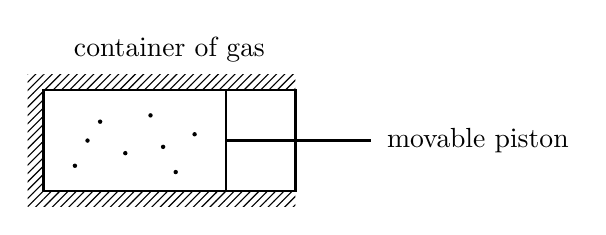
\begin{tikzpicture}[scale=0.8]
  \draw[thick] (0,0) rectangle (4,1.6);
  \fill[pattern=north east lines] (0,1.6) rectangle (4,1.85);
  \fill[pattern=north east lines] (0,-0.25) rectangle (4,0);
  \fill[pattern=north east lines] (-0.25,-0.25) rectangle (0,1.85);
  \draw[thick] (2.9,0) -- (2.9,1.6);
  \draw[thick] (2.9,0.8) -- (5.2,0.8);
  \foreach \p in {(0.5,0.4),(0.9,1.1),(1.3,0.6),(1.7,1.2),(2.1,0.3),(2.4,0.9),(0.7,0.8),(1.9,0.7)}
    \fill \p circle (0.035);
  \node[anchor=west] at (5.3,0.8) {movable piston};
  \node[anchor=south] at (2,1.9) {container of gas};
\end{tikzpicture}
\diagramcaption{A gas in a container closed by a movable piston.}
\end{diagram}

Some reference temperatures:
\begin{equation}
  T_m^{\mathrm{H_2O}} = 0^\circ\text{C} = 273.15\ \text{K},\qquad
  T_b^{\mathrm{H_2O}} = 100^\circ\text{C} = 373.15\ \text{K}.
\end{equation}
Pressure: $p = 101$~kPa $= 1.01\times 10^5$~Pa $\simeq 1$~bar, where
Pa = Pascal = Newton/(meter)$^2$ = MKS unit of pressure.

For a magnetic system the variables are $T$ and $\mathbf{H}$, the external magnetic
field ($\mathbf{B}$). The effect of an applied external $\mathbf{H}$ field is
\begin{equation}
  M = \chi H \qquad\text{(paramagnet)}.
\end{equation}
A solenoid is used to control $\mathbf{H}\equiv\mathbf{B}$: vary the electrical
current $I$ through it to control $\mathbf{B}$.

Externally controlled quantities:
\begin{itemize}
  \item $T$, $p$ in a liquid--gas system;
  \item $T$, $\mathbf{H}$ in a magnetic system.
\end{itemize}
(Don't confuse $H$ = external magnetic field with the symbol $H\leftrightarrow\Ham$
for the Hamiltonian.)

\subsection{Phase transitions and order parameters}

A phase transition is an abrupt change in the properties of a system,
characterized by an order parameter.

For a solid--liquid--gas system the order parameter is $\Delta\rho$ = difference in
density, e.g.\ for liquid--gas, $\Delta\rho = \rho_{\mathrm{liq}}-\rho_{\mathrm{gas}}$,
etc. (For a solid--solid phase transition a related order parameter is the type of
crystal structure.)

For a magnetic system the generic order parameter is the spontaneous magnetization
\begin{equation}
  \mathbf{M}_{sp} = \lim_{\mathbf{H}\to 0}\mathbf{M}(\mathbf{H})
\end{equation}
(ferromagnetic if $\uparrow\uparrow\uparrow\uparrow$ order; antiferromagnetic if
$\uparrow\downarrow\uparrow\downarrow$ order, where $\mathbf{M}_{\text{staggered}}$ is
the order parameter).

\subsection{Phase diagrams}

Example: a gas--liquid--solid system.

\begin{diagram}
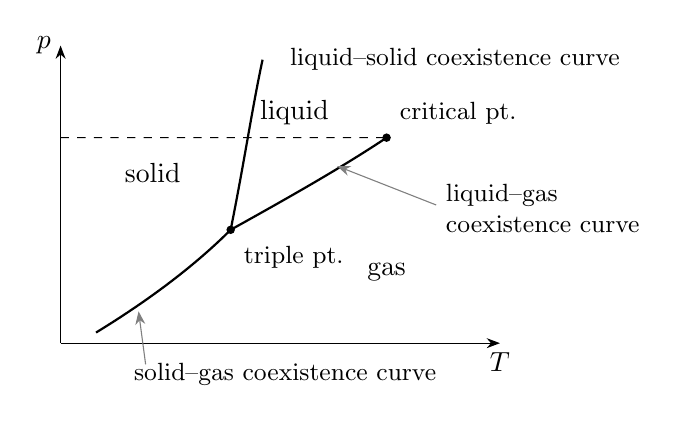
\begin{tikzpicture}[scale=0.9,>=Stealth]
  \draw[->] (0,0) -- (6.2,0) node[below] {$T$};
  \draw[->] (0,0) -- (0,4.2) node[left] {$p$};
  \coordinate (tp) at (2.4,1.6);
  \coordinate (cp) at (4.6,2.9);
  \draw[thick] (0.5,0.15) .. controls (1.4,0.7) and (2,1.2) .. (tp);
  \draw[thick] (tp) .. controls (3.3,2.1) and (4,2.5) .. (cp);
  \draw[thick] (tp) .. controls (2.6,2.6) and (2.7,3.3) .. (2.85,4);
  \fill (tp) circle (0.06);
  \fill (cp) circle (0.06);
  \draw[dashed] (0,2.9) -- (cp);
  \node at (1.3,2.4) {solid};
  \node at (3.3,3.25) {liquid};
  \node at (4.6,1.0) {gas};
  \node[anchor=south west,font=\small] at (4.65,2.95) {critical pt.};
  \node[anchor=north west,font=\small] at (2.45,1.5) {triple pt.};
  \node[anchor=west,font=\small,align=left] at (5.3,1.9) {liquid--gas\\ coexistence curve};
  \draw[->,gray] (5.3,1.95) -- (3.9,2.5);
  \node[anchor=west,font=\small] at (3.1,4) {liquid--solid coexistence curve};
  \node[anchor=north west,font=\small,align=left] at (0.9,-0.15) {solid--gas coexistence curve};
  \draw[->,gray] (1.2,-0.3) -- (1.1,0.45);
\end{tikzpicture}
\diagramcaption{Phase diagram of a solid--liquid--gas system. The critical point is
technically a ``bicritical point'', since one specifies two external variables,
temperature $T$ and pressure $p$, to reach this point.}\label{fig:pT}
\end{diagram}

The order parameter is $\Delta\rho_{\ell g}\equiv\rho_\ell-\rho_g$ for the
liquid--gas transition, and analogues for s--$\ell$, s--g.

Example: argon, $^{36}_{18}$Ar. As a noble gas, this has a rather simple phase
diagram. For Ar,
\begin{equation*}
\begin{aligned}
  T_m &= 83.81\ \text{K}, & T_b - T_m &= 3.49\ \text{K},\\
  T_b \equiv T_\ell &= 87.3\ \text{K}, & T_{cr} &= 150.39\ \text{K},\\
  T_{tr} &= 83.806\ \text{K}, & p_{cr} &= 4.86\ \text{MPa},\\
  p_{tr} &\simeq 69\ \text{kPa}, & 1\ \text{atm} &= 0.1\ \text{MPa}.
\end{aligned}
\end{equation*}
Comparison of $T_m$, $T_b$ with $^{20}_{10}$Ne (neon):
\begin{equation*}
  T_m = 24.56\ \text{K},\qquad T_b = 27.10\ \text{K},\qquad T_b - T_m = 2.54\ \text{K}.
\end{equation*}
For both Ar, Ne, etc., $T_b-T_m$ is only a few K, $\ll 100$~K for water.

\subsubsection*{Carbon dioxide}

Another example of a phase diagram for a s--$\ell$--gas system is carbon dioxide,
CO$_2$.

\begin{diagram}
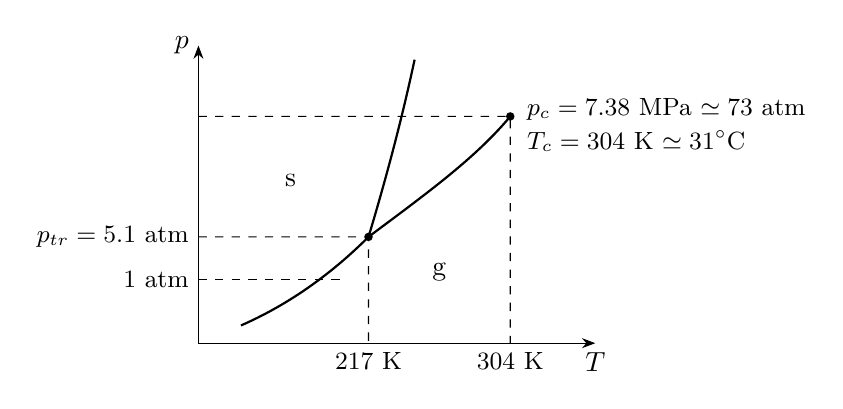
\begin{tikzpicture}[scale=0.9,>=Stealth]
  \draw[->] (0,0) -- (5.6,0) node[below] {$T$};
  \draw[->] (0,0) -- (0,4.2) node[left] {$p$};
  \coordinate (tp) at (2.4,1.5);
  \coordinate (cp) at (4.4,3.2);
  \draw[thick] (0.6,0.25) .. controls (1.4,0.6) and (2,1.1) .. (tp);
  \draw[thick] (tp) .. controls (3.2,2.1) and (3.9,2.6) .. (cp);
  \draw[thick] (tp) .. controls (2.7,2.5) and (2.9,3.3) .. (3.05,4);
  \fill (tp) circle (0.06); \fill (cp) circle (0.06);
  \draw[dashed] (0,3.2) -- (cp) -- (4.4,0);
  \draw[dashed] (0,1.5) -- (tp) -- (2.4,0);
  \draw[dashed] (0,0.9) -- (2.1,0.9);
  \node[left,font=\small] at (0,1.5) {$p_{tr}=5.1$ atm};
  \node[left,font=\small] at (0,0.9) {1 atm};
  \node[below,font=\small] at (2.4,0) {217 K};
  \node[below,font=\small] at (4.4,0) {304 K};
  \node at (1.3,2.3) {s};
  \node at (3.4,1.0) {g};
  \node[anchor=west,font=\small] at (4.5,3.3) {$p_c = 7.38$ MPa $\simeq 73$ atm};
  \node[anchor=west,font=\small] at (4.5,2.85) {$T_c = 304$ K $\simeq 31^\circ$C};
\end{tikzpicture}
\diagramcaption{Phase diagram of CO$_2$ (``dry ice'' for the solid). Since
$p_{tr}>1$~atm, the solid sublimates at atmospheric pressure.}
\end{diagram}

Interesting feature: CO$_2$ goes directly from solid $\to$ gas at $p = 1$~atm,
i.e.\ $p_{\text{triple}} > 1$~atm (sublimation). A nice demo: put dry ice in water
and see bubbles.

\subsubsection*{Water}

\begin{diagram}
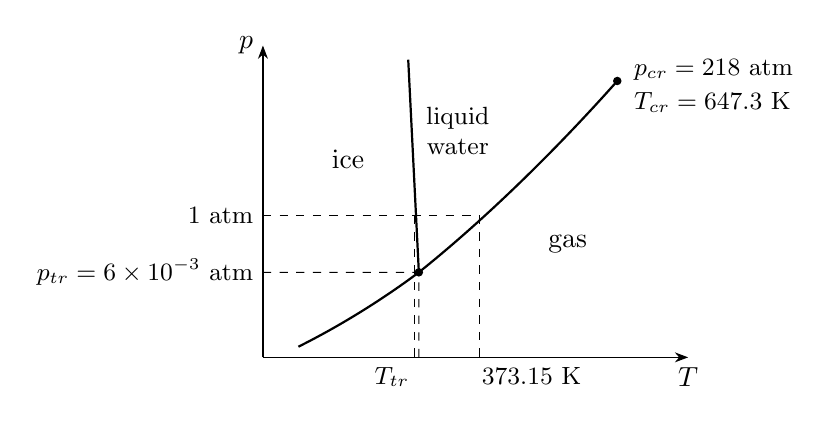
\begin{tikzpicture}[scale=0.9,>=Stealth]
  \draw[->] (0,0) -- (6,0) node[below] {$T$};
  \draw[->] (0,0) -- (0,4.4) node[left] {$p$};
  \coordinate (tp) at (2.2,1.2);
  \coordinate (cp) at (5,3.9);
  \draw[thick] (0.5,0.15) .. controls (1.2,0.5) and (1.8,0.9) .. (tp);
  \draw[thick] (tp) .. controls (3.2,2.0) and (4.2,3.0) .. (cp);
  \draw[thick] (tp) -- (2.05,4.2);
  \fill (tp) circle (0.06); \fill (cp) circle (0.06);
  \draw[dashed] (0,1.2) -- (tp) -- (2.2,0);
  \draw[dashed] (0,2.0) -- (3.05,2.0);
  \draw[dashed] (2.14,2.0) -- (2.14,0);
  \draw[dashed] (3.05,2.0) -- (3.05,0);
  \node[left,font=\small] at (0,2.0) {1 atm};
  \node[left,font=\small] at (0,1.2) {$p_{tr} = 6\times 10^{-3}$ atm};
  \node[below left,font=\small] at (2.2,0) {$T_{tr}$};
  \node[below right,font=\small] at (2.95,0) {373.15 K};
  \node at (1.2,2.8) {ice};
  \node[align=center,font=\small] at (2.75,3.2) {liquid\\ water};
  \node at (4.3,1.6) {gas};
  \node[anchor=west,font=\small] at (5.1,4.05) {$p_{cr} = 218$ atm};
  \node[anchor=west,font=\small] at (5.1,3.6) {$T_{cr} = 647.3$ K};
\end{tikzpicture}
\diagramcaption{Phase diagram of H$_2$O, with $T_m = 273.15\ \text{K} = 0^\circ$C,
$T_{tr} = 273.16$~K and $T_b = 373.15\ \text{K} = 100^\circ$C.}
\end{diagram}

For water, $T_b - T_m = 100$~K: a very large temperature interval over which water is
liquid. This is attributed to the large permanent electric dipole moment of water.
Water ice has many crystallographic structures; see the quantitative plots on
Blackboard.

\subsubsection*{Magnetic system}

\begin{diagram}
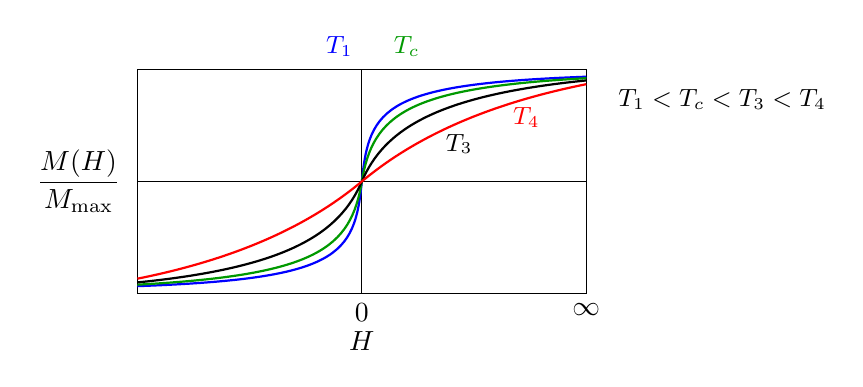
\begin{tikzpicture}[scale=0.95,>=Stealth]
  \draw (0,0) rectangle (6,3);
  \draw (0,1.5) -- (6,1.5);
  \draw (3,0) -- (3,3);
  \node[below] at (3,0) {$0$};
  \node[below] at (6,0) {$\infty$};
  \node[below=10pt] at (3,0) {$H$};
  \node[left] at (-0.1,1.5) {$\dfrac{M(H)}{M_{\max}}$};
  \draw[thick,blue] (0,0.1) .. controls (2.7,0.2) and (2.9,0.5) .. (3,1.5) .. controls (3.1,2.5) and (3.3,2.8) .. (6,2.9);
  \draw[thick,green!60!black] (0,0.12) .. controls (2.4,0.25) and (2.85,0.6) .. (3,1.5) .. controls (3.15,2.4) and (3.6,2.75) .. (6,2.88);
  \draw[thick] (0,0.15) .. controls (2,0.35) and (2.7,0.8) .. (3,1.5) .. controls (3.3,2.2) and (4,2.65) .. (6,2.85);
  \draw[thick,red] (0,0.2) .. controls (1.5,0.5) and (2.4,1.0) .. (3,1.5) .. controls (3.6,2.0) and (4.5,2.5) .. (6,2.8);
  \node[blue,font=\small] at (2.7,3.3) {$T_1$};
  \node[green!60!black,font=\small] at (3.6,3.3) {$T_c$};
  \node[font=\small] at (4.3,2.0) {$T_3$};
  \node[red,font=\small] at (5.2,2.35) {$T_4$};
  \node[anchor=west,font=\small] at (6.3,2.6) {$T_1<T_c<T_3<T_4$};
\end{tikzpicture}
\diagramcaption{Magnetization of a ferromagnet as a function of applied field $H$
for temperatures below, at and above $T_c$.}
\end{diagram}

The order parameter is the spontaneous magnetization
\begin{equation}
  M_{sp} = |\mathbf{M}_{sp}| = \lim_{|\mathbf{H}|\to 0}\mathbf{M}(\mathbf{H}).
\end{equation}

\begin{diagram}
\begin{tikzpicture}[scale=0.9,>=Stealth]
  \draw (0,0) -- (5,0); \draw (0,0) -- (0,3);
  \node[below] at (0,0) {$0$};
  \node[below] at (5,0) {$\infty$};
  \node[below] at (3,0) {$T_c$};
  \node[left] at (0,2) {$M_{sp}$};
  \draw[thick] (0,2.6) -- (1,2.6) .. controls (2.2,2.55) and (2.9,1.8) .. (3,0);
  \begin{scope}[xshift=7cm]
  \draw (0,0) -- (5,0); \draw (0,-0.8) -- (0,2.2);
  \node[left] at (0,1.6) {$H$};
  \draw[decorate,decoration={snake,amplitude=0.6pt,segment length=3pt},thick] (0,0) -- (2.4,0);
  \fill (2.4,0) circle (0.07);
  \node[blue,below] at (1.3,-0.1) {$T_1$};
  \node[green!60!black,below] at (2.4,-0.1) {$T_c$};
  \node[below] at (3.4,-0.1) {$T_3$};
  \node[red,below] at (4.4,-0.1) {$T_4$};
  \end{scope}
\end{tikzpicture}
\diagramcaption{Left: spontaneous magnetization as a function of $T$. Right: the
$(T,H)$ plane, with the phase boundary along $H=0$ for $0\le T<T_c$, ending at the
critical point.}
\end{diagram}

Relevant variables that specify a (bi)critical point:
\begin{itemize}
  \item s--$\ell$--g (solid--liquid--gas): $p = p_c$, $T = T_c$;
  \item magnetic: $H = H_c = 0$, $T = T_c$.
\end{itemize}
There is a discontinuous phase transition across a phase coexistence curve.

\subsection{Nonanalytic behavior and critical exponents}

A phase transition is signalled by nonanalytic behavior of thermodynamic
quantities.

For a solid--liquid--gas system, the Gibbs free energy is a function of $T$, $p$:
\begin{equation}
  G = G(T,p);\qquad
  \dd G = \underbrace{\left(\pder{G}{T}\right)_p}_{-S,\ \text{entropy}}\dd T
        + \underbrace{\left(\pder{G}{p}\right)_T}_{V,\ \text{volume}}\dd p.
\end{equation}
In a ``first-order'' phase transition, a first derivative of the free energy fails
to exist at $T_c$; here, there is a discontinuity in the volume $V$ occupied by a
given number $N$ of particles as a liquid transforms to a gas across the phase
boundary.

Example of a response function in a liquid--gas system:
\begin{equation}
  \kappa_T = -\frac{1}{V}\left(\pder{V}{p}\right)_T
  = -\frac{1}{V}\left(\frac{\partial^2 G}{\partial p^2}\right)_T
  = \text{isothermal compressibility},
\end{equation}
\begin{equation}
  \kappa_T \sim
  \begin{cases}
    \tau^{-\gamma} & \text{as } T\to T_c^+\\
    |\tau|^{-\gamma'} & \text{as } T\to T_c^-
  \end{cases}
  \qquad
  \tau = \frac{T-T_c}{T_c}.
\end{equation}
(Another common notation is $\epsilon = (T-T_c)/T_c$.)

At the critical point, $T = T_c$, $p = p_c$, the liquid--gas transition becomes
second-order, continuous. Similarly, in a magnetic system there is a critical point
at $T = T_c$, $H = H_c = 0$. For $G(T,H)$,
\begin{equation}
  \dd G = \underbrace{\left(\pder{G}{T}\right)_H}_{-S}\dd T
        + \underbrace{\left(\pder{G}{H}\right)_T}_{-M}\dd H
        = -S\,\dd T - M\,\dd H.
\end{equation}
The zero-field (``initial'') magnetic susceptibility
$\chi_0 = (\partial M/\partial H)_{H=0}$ is again a second derivative of $G$:
\begin{equation}
  \chi_0 = -\left(\frac{\partial^2 G}{\partial H^2}\right)_{H=0}.
\end{equation}
This exhibits non-analytic behavior, typically an algebraic divergence, described by
critical exponents $\gamma$, $\gamma'$:
\begin{equation}
  \chi_0\sim
  \begin{cases}
    \tau^{-\gamma} & \text{as } T\to T_c^+\quad\text{(leading singularity)}\\
    |\tau|^{-\gamma'} & \text{as } T\to T_c^-
  \end{cases}
\end{equation}
Usually $\gamma = \gamma'$. Other response functions behave similarly, such as the
specific heat $C_p = -T(\partial^2 G/\partial T^2)_p$:
\begin{equation}
  C_p\sim
  \begin{cases}
    \tau^{-\alpha} & \text{as } T\to T_c^+\\
    |\tau|^{-\alpha'} & \text{as } T\to T_c^-.
  \end{cases}
\end{equation}
The term ``second-order'' phase transition refers to the property that second-order
derivatives of the Gibbs free energy $G$ do not exist at this point, e.g.\ the
specific heat $C$ and (i) the compressibility for a liquid--gas transition; (ii) the
susceptibility for a magnetic transition.

\begin{diagram}
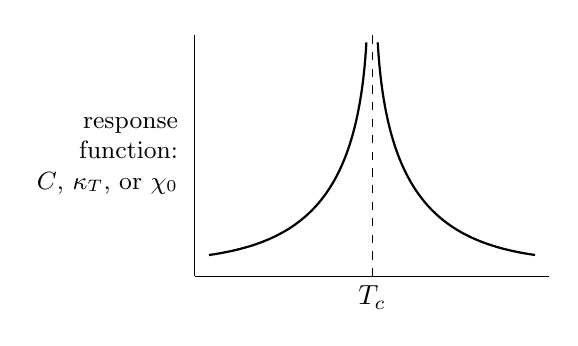
\begin{tikzpicture}[scale=0.9,>=Stealth]
  \draw (0,0) -- (5,0); \draw (0,0) -- (0,3.4);
  \draw[dashed] (2.5,0) -- (2.5,3.5);
  \draw[thick] (0.2,0.3) .. controls (1.6,0.5) and (2.3,1.2) .. (2.42,3.3);
  \draw[thick] (2.58,3.3) .. controls (2.7,1.2) and (3.4,0.5) .. (4.8,0.3);
  \node[below] at (2.5,0) {$T_c$};
  \node[left,align=right,font=\small] at (-0.1,1.7) {response\\ function:\\ $C$, $\kappa_T$, or $\chi_0$};
\end{tikzpicture}
\diagramcaption{Typical plot of a response function near $T_c$, with $\gamma=\gamma'$.}
\end{diagram}

Writing the response function as
\begin{equation}
  \begin{cases}
    A_+\tau^{-\gamma} & \text{for } T\to T_c^+\\
    A_-|\tau|^{-\gamma'} & \text{for } T\to T_c^-,
  \end{cases}
\end{equation}
the ``critical amplitudes'' $A_+\neq A_-$. See Figs.~1.13 and 1.16 in the book by
Stanley, \emph{Introduction to Phase Transitions and Critical Phenomena}. Of course,
experimentally we never actually observe $C\to\infty$ or $\chi\to\infty$, just large
values at $T_c$.

% Source: Lecture2.pdf, pages 2-4 (page 1 is a stray cover image, not notes).
\lecture{2}
\subsubsection*{Liquid--gas and solid--liquid systems}

We continue the introduction to phase transitions with the solid--liquid--gas
(s--$\ell$--g) system. The order parameter is
\begin{equation}
  \Delta\rho = \rho_\ell - \rho_g \quad\text{or}\quad \rho_s-\rho_\ell .
\end{equation}

\begin{diagram}
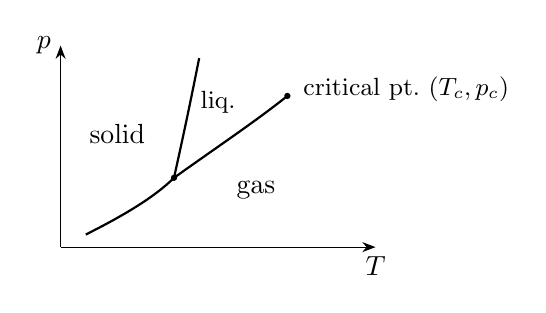
\begin{tikzpicture}[scale=0.8,>=Stealth]
  \draw[->] (0,0) -- (5,0) node[below] {$T$};
  \draw[->] (0,0) -- (0,3.2) node[left] {$p$};
  \coordinate (tp) at (1.8,1.1); \coordinate (cp) at (3.6,2.4);
  \draw[thick] (0.4,0.2) .. controls (1,0.5) and (1.5,0.8) .. (tp);
  \draw[thick] (tp) .. controls (2.5,1.6) and (3.1,2.0) .. (cp);
  \draw[thick] (tp) .. controls (2,2) and (2.1,2.5) .. (2.2,3);
  \fill (tp) circle (0.05); \fill (cp) circle (0.05);
  \node at (0.9,1.8) {solid};
  \node[font=\small] at (2.5,2.3) {liq.};
  \node at (3.1,0.9) {gas};
  \node[anchor=west,font=\small] at (3.7,2.5) {critical pt.\ $(T_c,p_c)$};
\end{tikzpicture}
\diagramcaption{The solid--liquid--gas phase diagram.}
\end{diagram}

There are discontinuities across first-order phase boundaries, i.e.\ phase
coexistence curves. Consider heating a solid, e.g.\ H$_2$O:
\begin{equation}
  C_p = \left.\frac{\dd U}{\dd T}\right|_p ;
\end{equation}
we add heat energy and raise $T$, approaching $T_\ell$. For ice,
$C_p\sim 0.5\ \text{cal/g}$ (recall: $1\ \text{cal} = 4.186$~J).

Going from solid to liquid: at $T = T_\ell = 0^\circ$C we must add energy while $T$ is
unchanged. For H$_2$O,
\begin{equation}
  L_m = 79.7\ \frac{\text{cal}}{\text{g}} = 3.33\times 10^2\ \frac{\text{J}}{\text{g}}.
\end{equation}
Next, heat the liquid water, with $C_p$ = specific heat of liquid water
$= 1$~cal/g. Then, as the temperature reaches $T_v$ ($T_v = 100^\circ\text{C} = 373$~K
at $p = 1$~atm), again one must add $L_v$ = ``latent heat of vaporization'' to convert
the system from a liquid to a gas:
\begin{equation}
  L_v = 539\ \text{cal/g} = 2.26\times 10^3\ \text{J/g}.
\end{equation}
These values of $L_m$ and $L_v$ for water are larger than for other substances, e.g.\
for nitrogen, N$_2$:
\begin{equation}
  L_m = 6.1\ \text{cal/g},\quad T_m = 63.2\ \text{K at } p = 1\ \text{atm};\qquad
  L_v = 48\ \text{cal/g},\quad T_v = 77.3\ \text{K}.
\end{equation}

\subsubsection*{The critical point and critical singularities}

At the critical point there is a continuous phase transition (p.t.):
\begin{itemize}
  \item $G(T,p)$, liquid--gas system, at $p = p_c$, $T = T_c$;
  \item $G(T,H)$, magnetic system, at $H = H_c = 0$, $T = T_c$;
\end{itemize}
with nonanalytic behavior as a function of $T$ and the other variable ($p$ or $H$).
(Watch videos on pressure cells.)

Critical singularities:
\begin{itemize}
  \item specific heat:
  \begin{equation}
    C\sim
    \begin{cases}
      \tau^{-\alpha} & T\searrow T_c\\
      (-\tau)^{-\alpha'} & T\nearrow T_c
    \end{cases}
    \qquad\text{where}\quad \tau = \frac{T-T_c}{T_c}
  \end{equation}
  (some authors use $\epsilon\equiv\tau$);
  \item liquid--gas compressibility $\kappa = -(1/V)\left(\partial V/\partial p\right)_T$
    and magnetic susceptibility $\chi = \left(\partial M/\partial H\right)_T$:
  \begin{equation}
    \kappa,\ \chi\sim
    \begin{cases}
      \tau^{-\gamma} & T\searrow T_c\\
      (-\tau)^{-\gamma'} & T\nearrow T_c.
    \end{cases}
  \end{equation}
\end{itemize}

Order parameter: for a magnetic system, $M_{sp} = \lim_{H\to 0}M(H)$, with
\begin{equation}
  M_{sp}\sim(-\tau)^{\beta}\quad\text{as } \tau\to 0^-
\end{equation}
(don't confuse the critical exponent $\beta$ with $\beta = 1/(\kB T)$). For a
liquid--gas system, $\Delta\rho = \rho_\ell-\rho_g$ and
$\Delta\rho\sim(-\tau)^{\beta}$.

\begin{diagram}
\begin{tikzpicture}[scale=0.8]
  \draw (0,0) -- (4,0); \draw (0,0) -- (0,2.4);
  \node[left] at (0,1.6) {$M_{sp}$};
  \node[below] at (2.8,0) {$T_c$};
  \node[below] at (1,0) {$T$};
  \draw[thick] (0,2) .. controls (1.6,2) and (2.7,1.5) .. (2.8,0);
\end{tikzpicture}
\diagramcaption{The order parameter vanishes continuously as $T\to T_c^-$.}
\end{diagram}

\subsubsection*{Correlation functions and the correlation length}

A measure of ordering is the two-point correlation function:
\begin{align*}
  \text{liquid--gas:}&\quad\ev{\Delta\rho(\mathbf{x})\,\Delta\rho(\mathbf{y})}_{\text{conn}},\\
  \text{magnetic:}&\quad\ev{\mathbf{S}(\mathbf{x})\cdot\mathbf{S}(\mathbf{y})}_{\text{conn}}
  \quad\text{or Ising}\quad \ev{\sigma(\mathbf{x})\,\sigma(\mathbf{y})}_{\text{conn}},
\end{align*}
with asymptotic decay as $|\mathbf{x}-\mathbf{y}|\to\infty$
\begin{equation}
  \sim\exp\left[-|\mathbf{x}-\mathbf{y}|/\xi\right],\qquad \xi = \text{correlation length}.
\end{equation}
(There can be a power-law prefactor also.) The decay of short-range order at large
distance is characterized by the correlation length $\xi$. For $T\to\infty$, spins are
uncorrelated: $\ev{\sigma(\mathbf{x})\sigma(\mathbf{y})} = 0$ if $\mathbf{x}\ne\mathbf{y}$.
Now decrease $T$. As $T$ approaches $T_c$, the correlation length $\xi\to\infty$ in a
second-order phase transition. The critical singularity in $\xi$ is
\begin{equation}
  \xi\sim
  \begin{cases}
    \tau^{-\nu} & T\searrow T_c\\
    (-\tau)^{-\nu'} & T\nearrow T_c,
  \end{cases}
  \qquad \xi\to\infty\ \text{at } T_c.
\end{equation}
(In actual substances $\xi$ does not $\to\infty$, but is $\gg$ the interatomic spacing,
so approximately $\to\infty$.)

Definition: the connected two-point function is
\begin{equation}
  \ev{\mathbf{S}(\mathbf{x})\cdot\mathbf{S}(\mathbf{y})}_{\text{conn}}
  \equiv \ev{\mathbf{S}(\mathbf{x})\cdot\mathbf{S}(\mathbf{y})} - \ev{\mathbf{S}}^2 .
\end{equation}
This is the same as the full two-point function above $T_c$, where
$|\ev{\mathbf{S}}| = |\mathbf{M}_{sp}| = 0$.

\subsubsection*{Quantities at the critical point}

At $T_c$, along the ``critical isotherm'' for the order parameter,
\begin{equation}
  |\mathbf{M}(\mathbf{H})|\sim|\mathbf{H}|^{1/\delta},\qquad
  \Delta\rho\sim|p-p_c|^{1/\delta},
\end{equation}
and
\begin{equation}
  \left.
  \begin{array}{l}
    \ev{\mathbf{S}(\mathbf{x})\cdot\mathbf{S}(\mathbf{y})}\\[2pt]
    \ev{\sigma(\mathbf{x})\,\sigma(\mathbf{y})}
  \end{array}\right\}
  \sim\frac{1}{|\mathbf{x}-\mathbf{y}|^{d-2+\eta}},
\end{equation}
where $d$ = spatial dimensionality.

\begin{diagram}
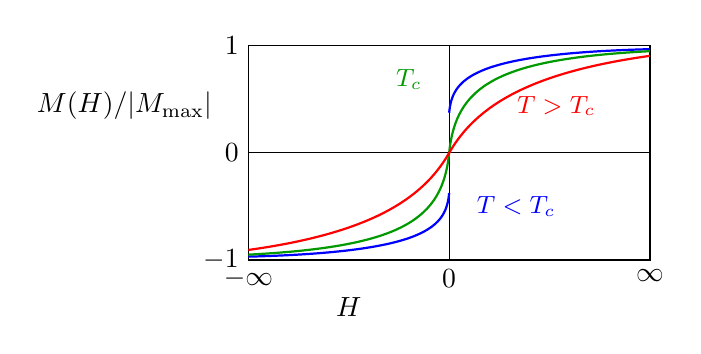
\begin{tikzpicture}[scale=0.85]
  \draw (0,0) rectangle (6,3.2);
  \draw (0,1.6) -- (6,1.6); \draw (3,0) -- (3,3.2);
  \node[below] at (0,0) {$-\infty$}; \node[below] at (3,0) {$0$}; \node[below] at (6,0) {$\infty$};
  \node[below=10pt] at (1.5,0) {$H$};
  \node[left] at (0,3.2) {$1$}; \node[left] at (0,1.6) {$0$}; \node[left] at (0,0) {$-1$};
  \node[left] at (-0.4,2.3) {$M(H)/|M_{\max}|$};
  \draw[thick,blue] (0,0.05) .. controls (2.7,0.12) and (2.95,0.5) .. (3,1.0);
  \draw[thick,blue] (3,2.2) .. controls (3.05,2.7) and (3.3,3.08) .. (6,3.15);
  \draw[thick,green!60!black] (0,0.08) .. controls (2.3,0.2) and (2.9,0.6) .. (3,1.6) .. controls (3.1,2.6) and (3.7,3.0) .. (6,3.12);
  \draw[thick,red] (0,0.15) .. controls (1.8,0.4) and (2.6,0.9) .. (3,1.6) .. controls (3.4,2.3) and (4.2,2.8) .. (6,3.05);
  \node[green!60!black,font=\small] at (2.4,2.7) {$T_c$};
  \node[red,font=\small] at (4.6,2.3) {$T>T_c$};
  \node[blue,font=\small] at (4,0.8) {$T<T_c$};
\end{tikzpicture}
\diagramcaption{Magnetization isotherms. For $T<T_c$ the magnetization jumps across
$H=0$; at $T=T_c$ it rises as $|H|^{1/\delta}$.}
\end{diagram}

Summary of critical exponents at a second-order phase transition:
$\{\alpha,\beta,\gamma,\nu\}$ and $\{\alpha',\gamma',\nu'\}$ for $T\ne T_c$,
$T\to T_c$; and $\{\delta,\eta\}$ at $T = T_c$.

\subsubsection*{Universality}

An important property of critical behavior and the associated critical exponents is
universality: they are independent of the details of the system, and only depend on
(1) the dimensionality $d$; (2) the symmetry group of the Hamiltonian.

Guggenheim, J.\ Chem.\ Phys.\ \textbf{13}, 253 (1945): data on the liquid--gas
transition in various substances (Ne, Ar, Kr, Xe, N$_2$, O$_2$, CO, CH$_4$),
\begin{equation}
  \Delta\rho = \rho_\ell-\rho_g\sim(-\tau)^{\beta}\quad\text{as }\tau\to 0^-,
\end{equation}
with measured value $\beta\sim1/3$ for all of these gases.

\begin{diagram}
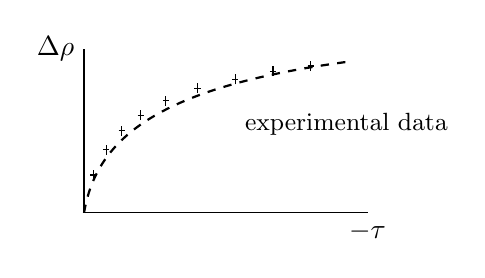
\begin{tikzpicture}[scale=0.8]
  \draw (0,0) -- (4.5,0) node[below] {$-\tau$};
  \draw (0,0) -- (0,2.6) node[left] {$\Delta\rho$};
  \draw[dashed,thick] (0,0) .. controls (0.2,1.2) and (1.2,2.0) .. (4.2,2.4);
  \foreach \x/\y in {0.15/0.6,0.35/1.0,0.6/1.3,0.9/1.55,1.3/1.78,1.8/1.98,2.4/2.12,3.0/2.25,3.6/2.33}
    \draw (\x-0.05,\y) -- (\x+0.05,\y) (\x,\y-0.08) -- (\x,\y+0.08);
  \node[anchor=west,font=\small] at (2.4,1.4) {experimental data};
\end{tikzpicture}
\diagramcaption{$\Delta\rho\sim(-\tau)^\beta$ fitted to liquid--gas data.}
\end{diagram}

E.g.\ Heller and Benedek (1962): similar universality was found in measurements of
$\beta$ for magnetic systems,
\begin{equation}
  M_{sp}\sim(-\tau)^{\beta}\quad\text{as }\tau\to 0^-
\end{equation}
(or $M_{\text{staggered}}$ for an antiferromagnet, $\uparrow\downarrow\uparrow\downarrow$),
so
\begin{equation}
  \ln M\sim\beta\ln(-\tau),\qquad \beta = \lim_{\tau\to 0^-}\frac{\ln M}{\ln(-\tau)}.
\end{equation}

\subsection{Physical scales and interatomic forces}
\subsubsection*{Sizes of relevant quantities}

Some sizes of relevant quantities in an atomic/molecular context, e.g.
\begin{equation}
  \hbar = 1.05\times 10^{-34}\ \text{J}\cdot\text{sec}
  = \frac{1.05\times 10^{-34}\ \text{J}\cdot\text{sec}}{1.60\times 10^{-19}\ \text{J/eV}}
  = 0.66\times 10^{-15}\ \text{eV-sec} = 0.66\ \text{eV-fs}
\end{equation}
($1\ \text{fs} = 10^{-15}$~sec). The value of $\hbar\sim(1\ \text{eV})(1\ \text{fs})\sim
\Order(1)$ in atomic-scale units.

For s--$\ell$--g phase transitions, $1\ \text{eV} = 1.60\times 10^{-19}$~Joules. The
product $\kB T$ is an energy; relate the MKS units to atomic/molecular units and
molecular bond strengths:
\begin{equation}
  \kB T = (1.38\times 10^{-23}\ \text{J/K})(1\ \text{K})
  = (0.862\times 10^{-4}\ \text{eV/particle})(1\ \text{Kelvin}).
\end{equation}
The bond strength for an ionic or covalent bond is
\begin{equation}
  \sim 100\ \text{kcal/mole} = \frac{(10^5)(4.186\ \text{J})}{(6.02\times 10^{23})(1.60\times 10^{-19}\ \text{J/eV})}
  = 4.35\ \text{eV/molecule}.
\end{equation}
N.B.: hydrogen bonds have strengths $\sim\Order(10)$ kcal/mol.

Pressure = force/area: $p = F/A = E/V$; the unit is Pa = N/m$^2$ (``Pascal''). Apply to
geophysics:
\begin{equation}
  (10\ \text{GPa})(10^{-10}\ \text{m})^3 = 10^{-20}\ \text{J}
  = \frac{10^{-20}\ \text{J}}{1.6\times 10^{-19}\ \text{J/eV}} = 6.3\times 10^{-2}\ \text{eV}.
\end{equation}

\begin{diagram}
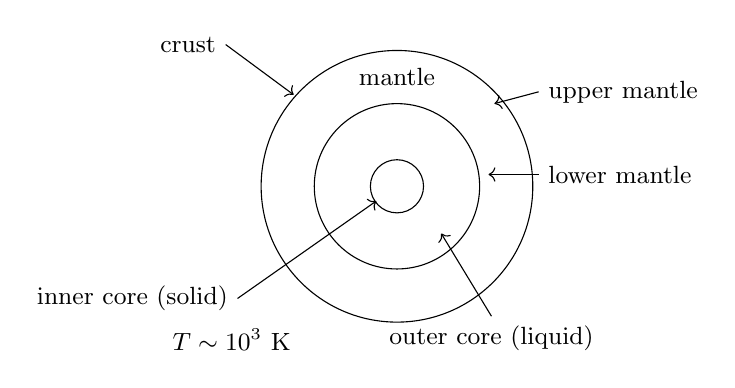
\begin{tikzpicture}[scale=0.75]
  \draw (0,0) circle (2.3);
  \draw (0,0) circle (1.4);
  \draw (0,0) circle (0.45);
  \draw[->] (-2.9,2.4) -- (-1.75,1.55); \node[anchor=east,font=\small] at (-2.9,2.4) {crust};
  \node[font=\small] at (0,1.85) {mantle};
  \draw[->] (2.4,1.6) -- (1.65,1.4); \node[anchor=west,font=\small] at (2.4,1.6) {upper mantle};
  \draw[->] (2.4,0.2) -- (1.55,0.2); \node[anchor=west,font=\small] at (2.4,0.2) {lower mantle};
  \draw[->] (-2.7,-1.9) -- (-0.35,-0.25); \node[anchor=east,font=\small] at (-2.7,-1.9) {inner core (solid)};
  \draw[->] (1.6,-2.2) -- (0.75,-0.8); \node[anchor=north,font=\small] at (1.6,-2.2) {outer core (liquid)};
  \node[font=\small] at (-2.8,-2.6) {$T\sim 10^3$ K};
\end{tikzpicture}
\diagramcaption{Layers of the earth.}
\end{diagram}

Here $1\ \text{atm} = 1\ \text{bar} = 100\ \text{kPa} = 0.1$~MPa. Typical values of
pressure in the earth (these pressures, and the associated temperatures, affect phase
changes in the rock):
\begin{itemize}
  \item $10$~kbar $= 1$~GPa: uppermost mantle;
  \item $\sim 100$~kbar $= 10$~GPa: upper mantle;
  \item $\sim 200$~kbar at the boundary between upper and lower mantle;
  \item $1.3$~Mbar $= 130$~GPa at the boundary between lower mantle and outer core;
  \item $3.3$~Mbar $= 330$~GPa at the boundary between outer (liquid) and inner (solid)
    core.
\end{itemize}
The phase transitions that occur in the rock in the interior of the earth involve
changes in crystal structure at high pressures and temperatures, i.e.\ solid--solid
phase transitions. At the boundary between the outer and inner core, there is a
liquid--solid phase transition. These properties were measured using seismology:
shear (transverse) waves travel through solids (at different speeds depending on
density), but not through liquid, while P (pressure, longitudinal) waves travel
through both solid and liquid.

% Source: Lecture3.pdf, page 1 (headed "Lecture 2A", rotated in the scan),
% pages 2-4 (Lecture 3); page 5 is blank.
\lecture{2A}
\subsubsection*{Pressure: high and low}

Continuation of the discussion of pressure:
\begin{equation}
  1\ \text{atm} \simeq 1\ \text{bar} = 0.1013\ \text{MPa} = 101.3\ \text{kPa}.
\end{equation}
Percy Bridgman (Harvard), in the 1920s and 1930s, achieved pressures of order
10~GPa, leading to the 1946 Nobel Prize. The DAC (diamond anvil cell) reached
$\Order(50)$--$\Order(100)$~GPa in the 1970s and 1980s; Silvera (Harvard)
$\to\Order(500\ \text{GPa})$.

Some relevant units. Torricelli: $1\ \text{torr} = 133\ \text{Pa} = 1$~mm of Hg in a
manometer (mercury is a convenient liquid to use in a manometer), and
\begin{equation}
  1\ \text{atm} = 760\ \text{mm Hg} = 760\ \text{torr} \simeq 30''\ \text{Hg}.
\end{equation}
Low pressure, vacuum conditions:
\begin{center}
\begin{tabular}{ll}
  $1$--$10^{-3}$ torr & rough vacuum\\
  $10^{-3}$--$10^{-5}$ torr & intermediate vacuum\\
  $10^{-5}$--$10^{-8}$ torr & high vacuum\\
  $10^{-8}$--$10^{-10}$ torr & very high vacuum\\
  $10^{-10}$--$10^{-12}$ torr & ultra-high vacuum
\end{tabular}
\end{center}
Applications: e.g.\ in particle physics (colliding beam machines) and studies of clean
surfaces in condensed matter physics.

\lecture{3}
\subsubsection*{Physical mechanism for liquefaction of a gas}

Next, we discuss the physical mechanism for liquefaction of a gas. Recall that the
atomic (also molecular) length scale is set by the Bohr length $a_B$:
\begin{equation}
  a_B = \frac{\hbar}{\alpha m_e c}\simeq 0.53\ \text{\AA} = 0.053\ \text{nm}.
\end{equation}
The dipole field is
\begin{equation}
  \mathbf{E}_d(\mathbf{r}) = \frac{3(\mathbf{d}\cdot\hat{\mathbf{r}})\hat{\mathbf{r}}-\mathbf{d}}{r^3},
  \qquad |\mathbf{d}|\sim e a_B,
\end{equation}
with fluctuation time scale $\sim 10^{-15}$~sec, since $\hbar\sim\Order(1)$~eV-fs.

The fluctuations in the electric charge distribution in a given atom produce a dipole
electric field $\mathbf{E}_d$ which induces a dipole moment in a neighboring atom, and
therefore there is an associated interaction energy $U$, with
$d_{\text{induced}}\sim a_B^3E_d\sim a_B^3\cdot ea_B/r^3 = ea_B^4/r^3$:
\begin{equation}
  U = -\mathbf{d}_{\text{induced}}\cdot\mathbf{E}_d
  = -\left(\frac{ea_B^4}{r^3}\right)\left(\frac{ea_B}{r^3}\right)
  = -\frac{e^2a_B^5}{r^6}\sim-\frac{e^2}{a_B}\left(\frac{a_B}{r}\right)^6
  \qquad\text{(CGS)}.
\end{equation}
This is an attraction, because the energy is negative and it gets more negative as the
distance $r$ gets smaller.

The van der Waals E.O.S.\ (equation of state) is
\begin{equation}
  \left(p + a\frac{N^2}{V^2}\right)(V-Nb) = N\kB T,\qquad \rho_n\equiv\frac{N}{V},
\end{equation}
where $Nb$ is the excluded-volume correction, $b\sim\Order(a_B^3)$. Dimensionally,
$p = F/A = E/V$, so
\begin{equation}
  \dim(a)\sim V^2\cdot\frac{E}{V} = E\cdot V\sim U_0\left\{\frac{4\pi}{3}r_0^3\right\},
\end{equation}
where $U_0$ and $r_0$ will be defined below.

This attractive interaction leads atoms (or molecules) to come closer. As the atoms (or
molecules) get so close that their electron clouds overlap, the Pauli Exclusion
Principle, which forbids identical fermions from occupying the same quantum state,
forces some electrons to move to higher-energy states, which costs energy. We can thus
deduce that the interaction energy will have a form, as a function of $r$, as shown in
the diagram.

\begin{diagram}
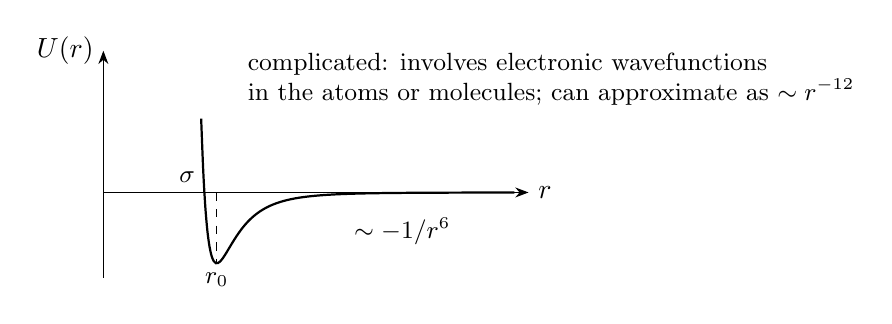
\begin{tikzpicture}[scale=0.9,>=Stealth]
  \draw[->] (0,0) -- (0,3.2) node[left] {$U(r)$};
  \draw[->] (0,1.2) -- (6,1.2) node[right] {$r$};
  \draw[thick,domain=1.38:5.8,samples=150,smooth]
    plot (\x,{min(3.1,1.2+1.0*((1.6/\x)^12-2*(1.6/\x)^6))});
  \draw (1.426,1.12) -- (1.426,1.28); \node[above left,font=\small] at (1.43,1.2) {$\sigma$};
  \draw[dashed] (1.6,1.2) -- (1.6,0.2); \node[below,font=\small] at (1.6,0.2) {$r_0$};
  \node[anchor=west,font=\small,align=left] at (1.9,2.8) {complicated: involves electronic wavefunctions\\
     in the atoms or molecules; can approximate as $\sim r^{-12}$};
  \node[anchor=west,font=\small] at (3.4,0.65) {$\sim -1/r^6$};
\end{tikzpicture}
\diagramcaption{The interatomic potential, with a hard core at short distance and an
attractive $r^{-6}$ tail.}
\end{diagram}

\subsubsection*{The Lennard-Jones potential}

The Lennard-Jones (6--12) energy $U(r)$ is
\begin{equation}
  U(r) = U_0\left[\left(\frac{r_0}{r}\right)^{12}-2\left(\frac{r_0}{r}\right)^{6}\right]
       \equiv 4U_0\left[\left(\frac{\sigma}{r}\right)^{12}-\left(\frac{\sigma}{r}\right)^{6}\right],
\end{equation}
with $r_0^6 = 2\sigma^6$, i.e.\ $r_0 = 2^{1/6}\sigma = 1.12\,\sigma$. The force is
$\mathbf{F} = -\boldsymbol{\nabla}U$; with $\mathbf{F} = F\hat{\mathbf{r}}$,
\begin{align}
  F &= -U_0\frac{\partial}{\partial r}\left[r_0^{12}r^{-12}-2r_0^6r^{-6}\right]
     = -U_0\left[-12r_0^{12}r^{-13}+12r_0^6r^{-7}\right]\nonumber\\
    &= \frac{12U_0}{r}\left[\left(\frac{r_0}{r}\right)^{12}-\left(\frac{r_0}{r}\right)^{6}\right];
\end{align}
$F = 0$ at $r = r_0$, the minimum of the potential.

E.g.\ Ar: $U_0/\kB = 120$~K, $r_0 = 3.8\ \text{\AA} = 0.38$~nm, with
\begin{equation*}
  T_\ell\equiv T_b = 87.5\ \text{K},\qquad T_m\equiv T_f = 84\ \text{K}
  \qquad(3.5\ \text{K difference}).
\end{equation*}
Here $T_\ell$ = liquefaction temperature $\equiv T_{\text{boil}}\equiv T_b$ and
$T_m = T_{\text{melt}}\equiv T_{\text{freeze}}$, at $p = 1$~atm.

Another example: CH$_4$ (methane). Symmetry implies $d = 0$ (no permanent electric
dipole):
\begin{equation*}
  T_\ell = T_b = 109\ \text{K},\qquad T_m = T_f = 90.7\ \text{K}.
\end{equation*}
CO$_2$ is a linear molecule; symmetry implies $d = 0$. The van der Waals analysis applies
not just to noble gas atoms (He, Ne, Ar, Kr, Xe), but more generally to atoms and
molecules (e.g.\ CH$_4$, CO$_2$) with $d = 0$.

Contrast with molecules that have permanent electric dipole moments, $d\sim ea_0$, e.g.\
H$_2$O (water), with $T_b - T_m = 100$~K, and ammonia NH$_3$. In both, the hydrogen side
carries charge $\delta+$ and the opposite side $\delta-$.

\subsection{Crystal structures and lattices}

Next, we discuss some crystal structures.

\begin{diagram}
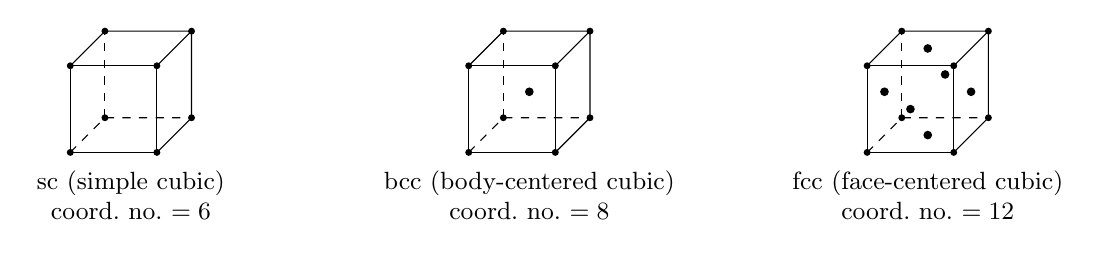
\begin{tikzpicture}[scale=1.1]
  \newcommand{\cube}{%
    \draw (0,0) rectangle (1,1);
    \draw (1,0) -- (1.4,0.4) -- (1.4,1.4) -- (1,1);
    \draw (0,1) -- (0.4,1.4) -- (1.4,1.4);
    \draw[dashed] (0,0) -- (0.4,0.4) -- (1.4,0.4);
    \draw[dashed] (0.4,0.4) -- (0.4,1.4);
    \foreach \p in {(0,0),(1,0),(0,1),(1,1),(0.4,0.4),(1.4,0.4),(0.4,1.4),(1.4,1.4)} \fill \p circle (0.04);}
  \begin{scope}\cube \node[below,align=center,font=\small] at (0.7,-0.1) {sc (simple cubic)\\ coord.\ no.\ $=6$}; \end{scope}
  \begin{scope}[xshift=4.6cm]\cube \fill (0.7,0.7) circle (0.05);
    \node[below,align=center,font=\small] at (0.7,-0.1) {bcc (body-centered cubic)\\ coord.\ no.\ $=8$}; \end{scope}
  \begin{scope}[xshift=9.2cm]\cube
    \foreach \p in {(0.5,0.5),(0.9,0.9),(0.7,0.2),(0.7,1.2),(0.2,0.7),(1.2,0.7)} \fill \p circle (0.05);
    \node[below,align=center,font=\small] at (0.7,-0.1) {fcc (face-centered cubic)\\ coord.\ no.\ $=12$}; \end{scope}
\end{tikzpicture}
\diagramcaption{Cubic lattices.}\label{fig:cubic}
\end{diagram}

The sc (simple cubic) lattice has coordination number 6. The coordination number of a
general $\mathbb{Z}^d$ lattice is $2d$. The coordination number of the bcc
(body-centered cubic) lattice is 8, and that of the fcc (face-centered cubic) lattice is
12.

Two-dimensional lattices:
\begin{itemize}
  \item square lattice, coordination number 4, denoted $4^4$. The square lattice is
    bipartite: $\Lambda_{sq} = \Lambda_e\oplus\Lambda_o$ (even, odd). More generally
    $\Lambda = \bigoplus_i\Lambda_i$.
  \item triangular (tri) lattice, coordination number 6, denoted $3^6$.
  \item honeycomb (hc) = hexagonal lattice, coordination number 3, denoted $6^3$; also
    bipartite, $\Lambda_{hc} = \Lambda_e\oplus\Lambda_o$.
\end{itemize}
These are the total set of homopolygonal 2D lattices.

The duality transformation $\Lambda\leftrightarrow\Lambda^*$ maps a face of $\Lambda$ to a
vertex on $\Lambda^*$, and hence a vertex on $\Lambda$ to a face on $\Lambda^*$; the bonds on
$\Lambda^*$ connect vertices in $\Lambda^*$.

\begin{diagram}
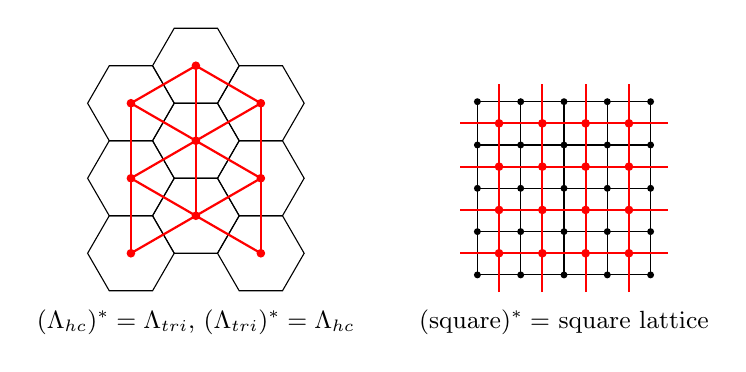
\begin{tikzpicture}[scale=0.55]
  % honeycomb with its dual triangular lattice
  \foreach \i in {0,1,2} \foreach \j in {0,1,2} {
    \pgfmathsetmacro{\cx}{1.5*\i}
    \pgfmathsetmacro{\cy}{sqrt(3)*\j + mod(\i,2)*sqrt(3)/2}
    \draw (\cx,\cy) +(0:1) -- +(60:1) -- +(120:1) -- +(180:1) -- +(240:1) -- +(300:1) -- cycle;
  }
  \foreach \i in {0,1,2} \foreach \j in {0,1,2} {
    \pgfmathsetmacro{\cx}{1.5*\i}
    \pgfmathsetmacro{\cy}{sqrt(3)*\j + mod(\i,2)*sqrt(3)/2}
    \fill[red] (\cx,\cy) circle (0.1);
  }
  \draw[red,thick] (0,0) -- (0,{sqrt(3)}) -- (0,{2*sqrt(3)});
  \draw[red,thick] (3,0) -- (3,{sqrt(3)}) -- (3,{2*sqrt(3)});
  \draw[red,thick] (1.5,{sqrt(3)/2}) -- (1.5,{3*sqrt(3)/2}) -- (1.5,{5*sqrt(3)/2});
  \draw[red,thick] (0,0) -- (1.5,{sqrt(3)/2}) -- (3,0);
  \draw[red,thick] (0,{sqrt(3)}) -- (1.5,{3*sqrt(3)/2}) -- (3,{sqrt(3)});
  \draw[red,thick] (0,{2*sqrt(3)}) -- (1.5,{5*sqrt(3)/2}) -- (3,{2*sqrt(3)});
  \draw[red,thick] (0,{sqrt(3)}) -- (1.5,{sqrt(3)/2}) -- (3,{sqrt(3)});
  \draw[red,thick] (0,{2*sqrt(3)}) -- (1.5,{3*sqrt(3)/2}) -- (3,{2*sqrt(3)});
  \node[font=\small] at (1.5,-1.6) {$(\Lambda_{hc})^* = \Lambda_{tri}$, $(\Lambda_{tri})^* = \Lambda_{hc}$};
  % square lattice and its dual
  \begin{scope}[xshift=8cm,yshift=-0.5cm]
    \foreach \x in {0,...,4} \draw (\x,0) -- (\x,4);
    \foreach \y in {0,...,4} \draw (0,\y) -- (4,\y);
    \foreach \x in {0,...,4} \foreach \y in {0,...,4} \fill (\x,\y) circle (0.08);
    \foreach \x in {0.5,1.5,2.5,3.5} \draw[red,thick] (\x,-0.4) -- (\x,4.4);
    \foreach \y in {0.5,1.5,2.5,3.5} \draw[red,thick] (-0.4,\y) -- (4.4,\y);
    \foreach \x in {0.5,1.5,2.5,3.5} \foreach \y in {0.5,1.5,2.5,3.5} \fill[red] (\x,\y) circle (0.1);
    \node[font=\small] at (2,-1.1) {$(\text{square})^* = $ square lattice};
  \end{scope}
\end{tikzpicture}
\diagramcaption{Duality transformation between the honeycomb and triangular lattices
(left), and the self-duality of the square lattice (right). The dual lattice is drawn
in red.}\label{fig:duality}
\end{diagram}

So the square lattice is self-dual.

There are also regular lattices composed of more than a single type of regular polygon;
these are called heteropolygonal. Example: the $4\cdot 8\cdot 8 = 4\cdot 8^2$
(``bathroom tile'') lattice.

\begin{diagram}
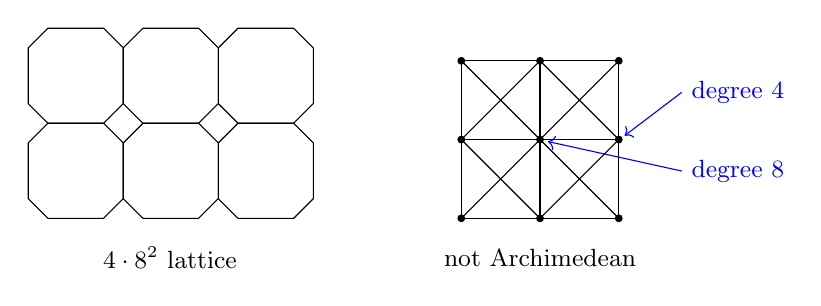
\begin{tikzpicture}[scale=0.5]
  \pgfmathsetmacro{\s}{1/(1+sqrt(2))}
  \foreach \i in {0,1,2} \foreach \j in {0,1} {
    \begin{scope}[shift={(2.414*\i,2.414*\j)}]
      \draw (0.5,0) -- (1.914,0) -- (2.414,0.5) -- (2.414,1.914) -- (1.914,2.414) -- (0.5,2.414) -- (0,1.914) -- (0,0.5) -- cycle;
    \end{scope}}
  \node[font=\small] at (3.6,-1) {$4\cdot 8^2$ lattice};
  \begin{scope}[xshift=11cm]
    \draw (0,0) rectangle (4,4);
    \draw (2,0) -- (2,4); \draw (0,2) -- (4,2);
    \draw (0,0) -- (4,4); \draw (0,4) -- (4,0);
    \draw (0,2) -- (2,4) -- (4,2) -- (2,0) -- cycle;
    \foreach \x in {0,2,4} \foreach \y in {0,2,4} \fill (\x,\y) circle (0.1);
    \draw[->,blue] (5.6,3.2) -- (4.15,2.1); \node[anchor=west,blue,font=\small] at (5.6,3.2) {degree 4};
    \draw[->,blue] (5.6,1.2) -- (2.2,1.95); \node[anchor=west,blue,font=\small] at (5.6,1.2) {degree 8};
    \node[font=\small] at (2,-1) {not Archimedean};
  \end{scope}
\end{tikzpicture}
\diagramcaption{Left: the heteropolygonal $4\cdot 8^2$ (``bathroom tile'') lattice.
Right: an example of a planar lattice that is not Archimedean, since some vertices
have degree 4 and others degree 8.}\label{fig:488}
\end{diagram}

Definition: an \emph{Archimedean lattice} is a regular tiling of the plane with some set
of regular polygons such that every vertex is equivalent to every other vertex.

Synonymous terms (math = physics): vertex = site; edge = bond.

Definition: the \emph{degree} of a vertex is the number of edges (= bonds) connecting to
it.

% Source: Lecture4.pdf, pages 1-9.
\lecture{4}
\subsubsection*{Three-dimensional crystal structures}

Recall some 3D crystal structures (the cubic cells are drawn in
Figure~\ref{fig:cubic}):
\begin{center}
\begin{tabular}{lll}
  structure & coord.\ no. & \\ \hline
  simple cubic, sc & 6 & \\
  body-centered cubic, bcc & 8 & with a site in the middle of the cube\\
  face-centered cubic, fcc & 12 & with sites at the centers of the faces\\
  hexagonal close packed, hcp & 12 &
\end{tabular}
\end{center}
E.g.\ the solid phase of Ar, Ne at $p\sim 1$~atm is fcc.

\subsubsection*{Two-dimensional lattices}

The homopolygonal 2D lattices are the square lattice (sq), coordination number 4,
$(4^4)$; the triangular lattice (tri), coordination number 6, $(3^6)$; and the
honeycomb (hc) or hexagonal lattice, coordination number 3, $(6^3)$. Some
heteropolygonal Archimedean lattices (2D) are the $(4\cdot 8\cdot 8)$ lattice,
coordination number 3, and the $(3\cdot 6\cdot 3\cdot 6)$ kagom\'e lattice,
coordination number 4.

\begin{diagram}
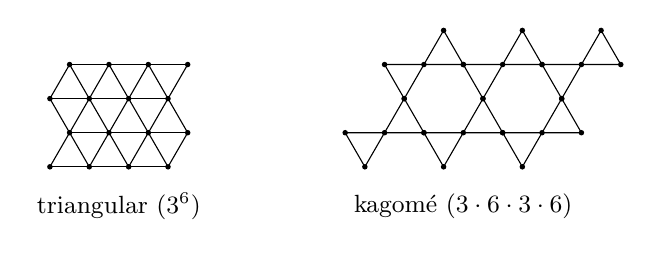
\begin{tikzpicture}[scale=0.5]
  % triangular
  \foreach \j in {0,1,2,3} \foreach \i in {0,1,2,3} {
    \pgfmathsetmacro{\x}{\i + 0.5*mod(\j,2)}
    \pgfmathsetmacro{\y}{0.866*\j}
    \fill (\x,\y) circle (0.07);
  }
  \foreach \j in {0,1,2,3} \draw ({0.5*mod(\j,2)},{0.866*\j}) -- ++(3,0);
  \foreach \i in {0,1,2,3} {\draw (\i,0) -- ++(60:1) -- ++(120:1) -- ++(60:1);}
  \foreach \i in {1,2,3} {\draw (\i,0) -- ++(120:1) -- ++(60:1) -- ++(120:1);}
  \node[font=\small] at (1.75,-1) {triangular $(3^6)$};
  % kagome: the medial graph of a triangular lattice of edge 2; corner-sharing triangles around hexagons
  \begin{scope}[xshift=7cm]
    \foreach \j in {0,1} \foreach \i in {0,1,2} {
      \begin{scope}[shift={(2*\i+\j,1.732*\j)}]
        \draw (1,0) -- (1.5,0.866) -- (0.5,0.866) -- cycle;
        \draw (1.5,0.866) -- (2.5,0.866) -- (2,1.732) -- cycle;
        \foreach \p in {(1,0),(0.5,0.866),(1.5,0.866),(2.5,0.866),(2,1.732)} \fill \p circle (0.07);
      \end{scope}}
    \node[font=\small] at (3.5,-1) {kagom\'e $(3\cdot 6\cdot 3\cdot 6)$};
  \end{scope}
\end{tikzpicture}
\diagramcaption{The triangular lattice and the kagom\'e lattice. The square,
honeycomb and $4\cdot 8^2$ lattices are drawn in Figures~\ref{fig:duality}
and~\ref{fig:488}.}
\end{diagram}

\subsection{Helium-4 and universality classes}
\subsubsection*{Helium-4}

Another phase diagram: $^4$He, the lightest noble element. This has the property that
there is no solid phase at pressure $p\sim 1$~atm; one has to increase $p\gtrsim 25$~atm
to get the $^4$He to solidify. This is due to large quantum zero-point motions of the He
atoms. Another important property is a phase transition (of second order) between a
normal liquid and a superfluid that flows without viscosity: a manifestation of
Bose--Einstein condensation.

\begin{diagram}
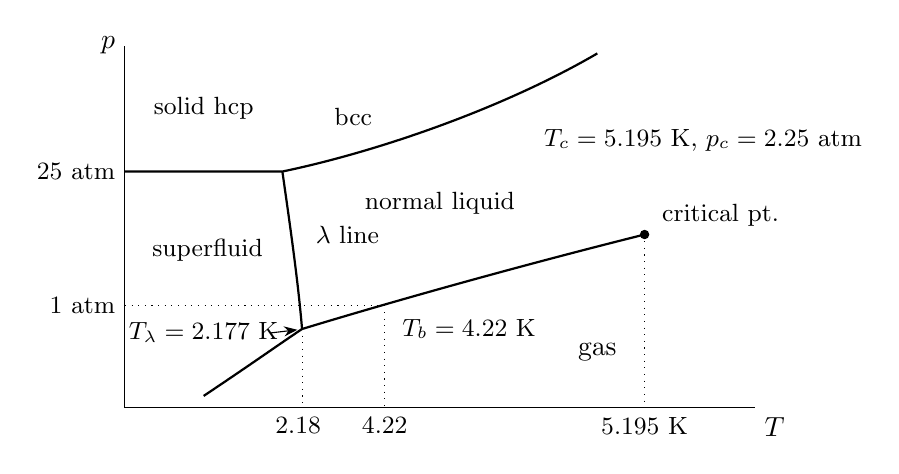
\begin{tikzpicture}[scale=1.0,>=Stealth]
  \draw (0,0) -- (8,0) node[below right] {$T$};
  \draw (0,0) -- (0,4.6) node[left] {$p$};
  % solid boundary at ~25 atm, lambda line, liquid-gas curve
  \draw[thick] (0,3.0) -- (2.0,3.0) .. controls (3.2,3.25) and (4.8,3.8) .. (6.0,4.5);
  \draw[thick] (2.0,3.0) .. controls (2.1,2.3) and (2.2,1.6) .. (2.25,1.0);
  \draw[thick] (1.0,0.15) .. controls (1.6,0.55) and (1.95,0.8) .. (2.25,1.0);
  \draw[thick] (2.25,1.0) .. controls (3.4,1.35) and (5.0,1.8) .. (6.6,2.2);
  \fill (6.6,2.2) circle (0.06);
  \draw[dotted] (0,1.3) -- (3.3,1.3);
  \draw[dotted] (2.25,1.0) -- (2.25,0); \draw[dotted] (3.3,1.3) -- (3.3,0); \draw[dotted] (6.6,2.2) -- (6.6,0);
  \node[left,font=\small] at (0,3.0) {25 atm};
  \node[left,font=\small] at (0,1.3) {1 atm};
  \node[below,font=\small] at (2.2,0) {2.18};
  \node[below,font=\small] at (3.3,0) {4.22};
  \node[below,font=\small] at (6.6,0) {5.195 K};
  \node[font=\small] at (1.0,3.8) {solid hcp};
  \node[font=\small] at (2.9,3.7) {bcc};
  \node[font=\small] at (1.05,2.0) {superfluid};
  \node[font=\small] at (4.0,2.6) {normal liquid};
  \node[font=\small,anchor=west] at (2.3,2.2) {$\lambda$ line};
  \node at (6.0,0.7) {gas};
  \node[anchor=west,font=\small] at (6.7,2.45) {critical pt.};
  \node[anchor=west,font=\small] at (5.2,3.4) {$T_c = 5.195$ K, $p_c = 2.25$ atm};
  \node[anchor=west,font=\small] at (3.4,1.0) {$T_b = 4.22$ K};
  \node[font=\small] at (1.0,0.95) {$T_\lambda = 2.177$ K}; \draw[->] (1.85,0.95) -- (2.19,0.99);
\end{tikzpicture}
\diagramcaption{Phase diagram of $^4$He ($T_b = 4.222$~K). The $\lambda$ line separates
the superfluid from the normal liquid.}
\end{diagram}

The ``$\lambda$'' line is named for the shape of the specific heat curve (see, e.g.,
Stanley, p.~20, Fig.~1.16).

\begin{diagram}
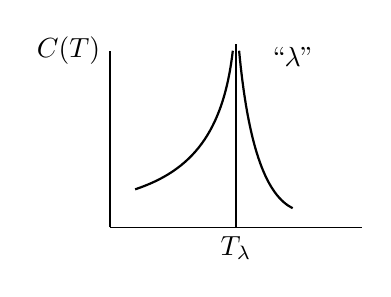
\begin{tikzpicture}[scale=0.8]
  \draw (0,0) -- (4,0); \draw (0,0) -- (0,2.8) node[left] {$C(T)$};
  \draw (2,0) -- (2,2.9);
  \draw[thick] (0.4,0.6) .. controls (1.3,0.9) and (1.8,1.5) .. (1.95,2.8);
  \draw[thick] (2.05,2.8) .. controls (2.2,1.2) and (2.5,0.5) .. (2.9,0.3);
  \node[below] at (2,0) {$T_\lambda$};
  \node at (2.9,2.7) {``$\lambda$''};
\end{tikzpicture}
\diagramcaption{The specific heat of $^4$He near $T_\lambda$.}
\end{diagram}

The physical origin of ferromagnetism is due to the Pauli Exclusion Principle: if spins
are aligned, then the electron clouds do not overlap, and the resultant separation
reduces the Coulomb energy due to e--e electrostatic repulsion. Antiferromagnetism occurs
due to a combination of this effect and spin interactions in compounds, e.g.\ MnO, etc.

\subsubsection*{Universality classes of phase transitions}

\paragraph{1. Uniaxial ferromagnet (Ising model), \texorpdfstring{$G = \mathbb{Z}_2$}{G = Z2}.}

\begin{equation}
  \Ham = -J\sum_{\langle ij\rangle}\sigma_i\sigma_j - \mu H\sum_i\sigma_i ,
\end{equation}
where $\sigma_i = \pm 1$ is a classical spin and $J$ is the spin--spin exchange
(coupling). Here $\mathbf{S}_i = (1/2)\boldsymbol{\sigma}_i$, and we absorb
$(1/2)^2$ into $J$. The second term comes from
$U_{\text{mag}} = -\boldsymbol{\mu}\cdot\mathbf{H}$; choose units such that $\mu = 1$.
\begin{itemize}
  \item $J>0\Rightarrow$ the spin--spin interaction favors parallel spins,
    $\uparrow\uparrow$: FM (ferromagnetic sign of the coupling).
  \item $J<0$ favors opposite orientations of nearest-neighbor (n.n.) spins,
    $\uparrow\downarrow$: AFM.
\end{itemize}
The symmetry (group) of this $\Ham$ with $H = 0$ (i.e.\ zero external magnetic field) is
$\mathbb{Z}_2$, generated by $\{1,-1\}$ (the identity, and $\uparrow\to\downarrow$). A
$\mathbb{Z}_2$ transformation reverses all spins (a global symmetry operation):
\begin{equation}
  \sigma_i\sigma_j\to(-\sigma_i)(-\sigma_j) = \sigma_i\sigma_j .
\end{equation}
This symmetry is explicitly broken if the external field $H\ne 0$. As $T\searrow T_c$
(given that $H = 0$) the $\mathbb{Z}_2$ symmetry is spontaneously broken by the onset of
a spontaneous magnetization.

\begin{diagram}
\begin{tikzpicture}[scale=0.8]
  \draw (0,0) -- (4,0); \draw (0,0) -- (0,2.4) node[left] {$M_{sp}(T)$};
  \draw[thick] (0,1.9) -- (0.9,1.9) .. controls (2.2,1.85) and (2.9,1.3) .. (3,0);
  \node[below] at (1,0) {$T$}; \node[below] at (3,0) {$T_c$};
\end{tikzpicture}
\diagramcaption{Onset of spontaneous magnetization below $T_c$.}
\end{diagram}

SSB = spontaneous symmetry breaking, associated with LRO = long-range order and a nonzero
value of the order parameter, which is the spontaneous magnetization.

\paragraph{2. Liquid--gas: an example of the \texorpdfstring{$\mathbb{Z}_2$}{Z2} universality class.}

The liquid--gas (also liquid--solid) phase transition. Imagine a formal lattice (the
lattice gas model of T.D.~Lee and C.N.~Yang). Say pressure $p$ is fixed. At $T>T_c$, the
probability of a molecule or atom being present at a site in the lattice gas is
$1/2$: random. As $T\searrow T_c$, the sites are occupied with probability $>1/2$.
As $T$ decreases further, this probability increases, $\to 1$.

\begin{diagram}
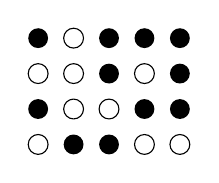
\begin{tikzpicture}[scale=0.45]
  \foreach \r/\row in {0/{1,0,1,1,1},1/{0,0,1,0,1},2/{1,0,0,1,1},3/{0,1,1,0,0}} {
    \foreach \v [count=\c] in \row {
      \ifnum\v=1 \fill (\c,-\r) circle (0.28); \else \draw (\c,-\r) circle (0.28); \fi
    }}
\end{tikzpicture}
\diagramcaption{A lattice gas: filled circles are occupied sites, open circles are
empty.}
\end{diagram}

The feature is yes/no with respect to occupation. It can be modelled as a phase
transition in the $\mathbb{Z}_2$ universality class. This model is justified a
posteriori by the agreement of the critical exponents calculated for a $\mathbb{Z}_2$
system and the experimentally measured values, e.g.\ recall the curve showing data at
$p_c$, $T_c$ for $\Delta\rho = \rho_\ell-\rho_g$ from Guggenheim.

\paragraph{3. \texorpdfstring{$O(N)$}{O(N)} spin models.}

For spin systems, we have (infinitely many) additional universality classes. Consider
the Hamiltonian
\begin{equation}
  \Ham = -J\sum_{\langle ij\rangle}\mathbf{S}_i\cdot\mathbf{S}_j
         - \mu\,\mathbf{H}\cdot\sum_i\mathbf{S}_i
\end{equation}
(again, choose units such that $\mu = 1$). Here $\mathbf{S}_i$ is a spin (a classical
vector with $|\mathbf{S}_i| = 1$, or quantum with $\|\mathbf{S}\|^2 = S(S+1)$, $\hbar = 1$)
with $N$ components, $\mathbf{S}_i = (S_{i,1},\ldots,S_{i,N})$.
\begin{itemize}
  \item $N = 3$ components: the Heisenberg model, $(S_{i,1},S_{i,2},S_{i,3})$. If
    $\mathbf{H} = 0$, the global symmetry group of $\Ham$ is $O(3)$.
  \item $O(2)$, $XY$, $N = 2$ components: $\mathbf{S}_i = (S_{i,1},S_{i,2})$. Here, as the
    name indicates, $G = O(2)$; the spin lives on $S^1$.
  \item In general, the $O(N)$ spin model. Recall that an $O(3)$ spin ``lives'' on $S^2$.
\end{itemize}
Definition: given a vector $\mathbf{x}\in\mathbb{R}^N$, the condition
$|\mathbf{x}| = \text{const.}$ defines the $(N-1)$-dimensional sphere $S^{N-1}$.

Similarly, for $O(N)$, $\mathbf{S}_i = (S_{i1},\ldots,S_{iN})$ with $|\mathbf{S}| = 1$
``lives'' on $S^{N-1}$, the $(N-1)$-sphere. A slice of the $S^2$ sphere is $\sim S^1$.
Similarly, a slice of $S^1$ is $\sim\mathbb{Z}_2$ (the two antipodal points in $S^1$). In
this sense, the Ising model is a member of the $O(N)$ series of models, corresponding to
$N = 1$.

An example of an $O(2)$ model: $O(2)\approx U(1)$, the group of elements $e^{\ii\theta}$
under multiplication, $e^{\ii\theta_1}\cdot e^{\ii\theta_2} = e^{\ii(\theta_1+\theta_2)}$.
In superconductivity the order parameter is the Cooper pair; in BCS theory
$\ev{ee}\sim\ev{\psi\psi}$, which has a complex phase. The superconducting phase
transition is in the $O(2)$ universality class. The normal fluid--superfluid phase
transition in $^4$He is also in the $O(2)\approx U(1)$ universality class; the order
parameter is the complex phase of the superfluid condensate wavefunction.

\paragraph{4. Structural transition in a binary alloy, \texorpdfstring{$\mathbb{Z}_2$}{Z2}.}

$\beta$ brass is an alloy of Cu and Zn (copper and zinc), on a body-centered cubic lattice.
At $T<T_c = 742$~K the Cu and Zn atoms are on the two interleaved sublattices. Recall
that the bcc lattice is bipartite, $\Lambda_{bcc} = \Lambda_e\oplus\Lambda_o$. As
$T\nearrow T_c$, the positions of the Cu and Zn atoms become increasingly random.

\begin{diagram}
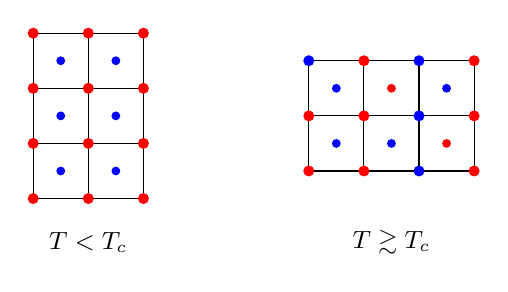
\begin{tikzpicture}[scale=0.7]
  \foreach \x in {0,1,2} \draw (\x,0) -- (\x,3);
  \foreach \y in {0,1,2,3} \draw (0,\y) -- (2,\y);
  \foreach \x in {0,1,2} \foreach \y in {0,1,2,3} \fill[red] (\x,\y) circle (0.1);
  \foreach \x in {0.5,1.5} \foreach \y in {0.5,1.5,2.5} \fill[blue] (\x,\y) circle (0.08);
  \node[font=\small,align=center] at (1,-0.8) {$T<T_c$};
  \begin{scope}[xshift=5cm,yshift=0.5cm]
    \foreach \x in {0,1,2,3} \draw (\x,0) -- (\x,2);
    \foreach \y in {0,1,2} \draw (0,\y) -- (3,\y);
    \foreach \x/\y/\c in {0/0/red,1/0/red,2/0/blue,3/0/red,0/1/red,1/1/red,2/1/blue,3/1/red,0/2/blue,1/2/red,2/2/blue,3/2/red}
      \fill[\c] (\x,\y) circle (0.1);
    \foreach \x/\y/\c in {0.5/0.5/blue,1.5/0.5/blue,2.5/0.5/red,0.5/1.5/blue,1.5/1.5/red,2.5/1.5/blue}
      \fill[\c] (\x,\y) circle (0.08);
    \node[font=\small] at (1.5,-1.3) {$T\gtrsim T_c$};
  \end{scope}
\end{tikzpicture}
\diagramcaption{Slices of the bcc lattice of $\beta$ brass, with Cu in red and Zn in
blue. Left: a portion of the bcc lattice at $T<T_c$. Right: a slice at $T\gtrsim T_c$,
showing the partial reduction in positional ordering.}
\end{diagram}

\paragraph{5. Liquid crystals.}

We will also consider other types of phase transitions. One example will involve
topological ordering: the liquid crystal isotropic--nematic transition.
\begin{itemize}
  \item Isotropic phase: no positional ordering and also no orientational ordering.
  \item Nematic phase: no positional ordering but $\exists$ orientational ordering.
\end{itemize}
The space of the order parameter for a liquid crystal is $S^2/\mathbb{Z}_2$, because the
ends of the rod-like molecules are equivalent, so we ``mod out'' $S^2$ by $\mathbb{Z}_2$.
(Contrast with a FM, where the spins carry arrows.)

\begin{diagram}
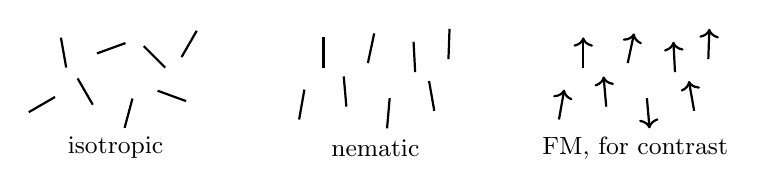
\begin{tikzpicture}[scale=0.55]
  \foreach \x/\y/\a in {0/0/30,1/0.3/120,2/-0.2/75,3/0.2/160,0.5/1.2/100,1.6/1.3/20,2.6/1.1/135,3.4/1.4/60}
    \draw[thick] (\x,\y) ++(\a:0.35) -- ++(\a+180:0.7);
  \node[font=\small] at (1.7,-1) {isotropic};
  \begin{scope}[xshift=6cm]
  \foreach \x/\y/\a in {0/0/80,1/0.3/95,2/-0.2/85,3/0.2/100,0.5/1.2/90,1.6/1.3/78,2.6/1.1/93,3.4/1.4/88}
    \draw[thick] (\x,\y) ++(\a:0.35) -- ++(\a+180:0.7);
  \node[font=\small] at (1.7,-1) {nematic};
  \end{scope}
  \begin{scope}[xshift=12cm]
  \foreach \x/\y/\a in {0/0/80,1/0.3/95,2/-0.2/-85,3/0.2/100,0.5/1.2/90,1.6/1.3/78,2.6/1.1/93,3.4/1.4/88}
    \draw[thick,->] (\x,\y) ++(\a+180:0.35) -- ++(\a:0.7);
  \node[font=\small] at (1.7,-1) {FM, for contrast};
  \end{scope}
\end{tikzpicture}
\diagramcaption{Rod-like molecules in the isotropic and nematic phases of a liquid
crystal, and spins in a ferromagnet.}
\end{diagram}

\subsubsection*{What determines the universality class}

So: the universality class of the critical point and associated second-order phase
transition is determined by
\begin{enumerate}[label=(\arabic*)]
  \item the symmetry group $G$ of the Hamiltonian $\Ham$;
  \item the spatial dimensionality of the lattice $\Lambda$.
\end{enumerate}
In the development of the theory of phase transitions and critical phenomena, this
notion of universality class was developed and tested by a combination of (a)
measurements on physical systems (recall the Guggenheim plot that showed the same
critical exponent $\beta$ for different gases, and similar measurements of different
magnetic systems); (b) approximate studies of model systems such as high-temperature
and low-temperature series expansions; (c) renormalization group analyses; (d) Monte
Carlo simulations.

Thus, for example, if we changed the Hamiltonian of the Ising model from
\begin{equation}
  \Ham = -J\sum_{\langle ij\rangle}\sigma_i\sigma_j - H\sum_i\sigma_i
\end{equation}
with, say, $J>0$ (FM), where $\langle ij\rangle$ are nearest-neighbor pairs of sites, to
include FM next-nearest-neighbor spin--spin interactions,
\begin{equation}
  \Ham_{nn+nnn} = -J_{nn}\sum_{\langle ij\rangle_{nn}}\sigma_i\sigma_j
                  - J_{nnn}\sum_{\langle k\ell\rangle_{nnn}}\sigma_k\sigma_\ell
                  - H\sum_i\sigma_i ,
\end{equation}
then the critical behavior is the same (again with $H = H_c = 0$), because the
$\mathbb{Z}_2$ (global) symmetry group of the zero-field $\Ham$ is the same and the
dimensionality of the lattice is, of course, unchanged. The $\Ham$ with nearest-neighbor
spin--spin interactions is a simplification, but usually a reasonably good one, since
interactions decrease as the distance between the spins (really the electron clouds)
increases.

Another condition to remain in the same universality class is that the additional
interactions are not ``competing interactions'' that introduce frustration. For example
if $J_{nn}>0$ (FM) but the nnn interaction had $J_{nnn}<0$ (AFM), this would be a
competing interaction: the $J_{nn}$ would favor spin alignment, but the $J_{nnn}$ would
favor antiparallel spin ordering, a conflicting tendency. This would lead to frustration
and would change the universality class.

One can also add multispin interactions such as 4-spin interactions involving the 4
spins on the sites of a square lattice (with $J_\square>0$ to avoid competing
interactions), to get
\begin{equation}
  \Ham = -J_{nn}\sum_{\langle ij\rangle}\sigma_i\sigma_j
         - J_\square\sum_{\square\ \text{squares}}\sigma_i\sigma_j\sigma_k\sigma_\ell
         - H\sum_i\sigma_i ,
\end{equation}
and again this maintains the same symmetry group $G = \mathbb{Z}_2$ (and dimension $d$ of
the lattice), so this does not change the universality class of the critical behavior
(with $H = H_c = 0$).

In contrast, say we add a 3-spin interaction on a square or along an axis of the
lattice. The associated term in $\Ham$, $-J_{3s}\sum\sigma_i\sigma_j\sigma_k$, is not
invariant under the $\mathbb{Z}_2$ symmetry group:
\begin{equation}
  \sigma_i\sigma_j\sigma_k\to(-1)^3\sigma_i\sigma_j\sigma_k = -\sigma_i\sigma_j\sigma_k
\end{equation}
under the group transformation, so this breaks the symmetry and does change the
universality class of the critical behavior.

\begin{diagram}
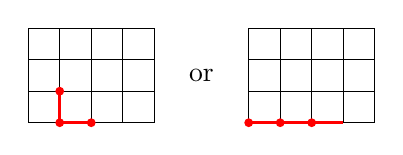
\begin{tikzpicture}[scale=0.4]
  \foreach \s in {0,7} {
  \begin{scope}[xshift=\s cm]
    \foreach \x in {0,...,4} \draw (\x,0) -- (\x,3);
    \foreach \y in {0,...,3} \draw (0,\y) -- (4,\y);
  \end{scope}}
  \draw[red,very thick] (1,1) -- (1,0) -- (2,0);
  \foreach \p in {(1,1),(1,0),(2,0)} \fill[red] \p circle (0.14);
  \draw[red,very thick] (7,0) -- (10,0);
  \foreach \p in {(7,0),(8,0),(9,0)} \fill[red] \p circle (0.14);
  \node at (5.5,1.5) {or};
\end{tikzpicture}
\diagramcaption{Three-spin interactions on a square or along a lattice axis.}
\end{diagram}

Other effects that can change the critical behavior include lattice defects and
impurities in the material (and these are important effects experimentally).

\subsubsection*{Classical and quantum spins}

A note on the basic physics: although we write the interaction term of a magnetic system
as $\Ham = -J\sum_{\langle ij\rangle}\sigma_i\sigma_j$ or
$-J\sum_{\langle ij\rangle}\mathbf{S}_i\cdot\mathbf{S}_j$, the underlying physics is the
Pauli exclusion principle, which for a FM prefers spin alignment to keep the spins apart
and hence reduce the Coulomb repulsion energy. The magnitude of the $J$ is thus set by
the electrostatic Coulomb interaction, not by the dipole--dipole interaction of
individual electrons, which is much smaller.

Another comment concerns the use of classical quantities in stat.\ mech.\ models. The
true interaction that is responsible for magnetic behavior involves quantum mechanics
(QM), and hence the spins are operators, and the Hamiltonian $\Ham$ is a quantum
mechanical operator, not a scalar. However, the behavior of the system can often be well
described by using classical spins. So for a magnet with a largely uniaxial effective
spin--spin interaction, we have
$(S_z)_i(S_z)_j = ((1/2)\sigma_z)_i((1/2)\sigma_z)_j$, and since
$\sigma_z = \left(\begin{smallmatrix}1&0\\0&-1\end{smallmatrix}\right)$, we can replace
these operators by just $\sigma_i\sigma_j$ when the $\sigma_i$ are classical variables
$=\pm 1$ (absorbing the prefactor of $(1/2)^2$ in $J$). Note that the QM commutation
relation
\begin{equation}
  [S_\alpha,S_\beta] = \ii\epsilon_{\alpha\beta\gamma}S_\gamma,\qquad
  \alpha,\beta,\gamma = x,y,z,
\end{equation}
means that $(S_z)_i$ and $(S_z)_j$ commute. This is also true when one has an external
magnetic field in the $\hat{\mathbf{z}}$ direction. Moreover, in the two other examples
of systems in the Ising universality class given above, namely the liquid--gas transition
and the structural phase transition of a binary alloy like brass, the variable
$\sigma_i = \pm 1$ (equivalently $(1+\sigma_i)/2 = 1$ or $0$) refers to an
occupation number, not a spin.

Example of a quantum spin system: the ``transverse Ising model'' with
\begin{equation}
  \Ham = -J\sum_{\langle ij\rangle}(\sigma_z)_i(\sigma_z)_j - \mu H_x\sum_i(\sigma_x)_i ,
\end{equation}
where one applies an external magnetic field transverse to the axis of quantization of
the interacting spins. Because of its complexity, one often studies it in one dimension,
as a ``quantum spin chain''. Studies go back to the 1920s and 1930s, e.g.\ by Bethe and
others. For examples, see, e.g.:
\begin{itemize}
  \item B.~McCoy, J.~Perk, R.~Shrock, Nucl.\ Phys.\ \textbf{B220}, 35 (1983);
    \textbf{B220}, 269 (1983);
  \item G.~M\"uller and R.~Shrock, Phys.\ Rev.\ Lett.\ \textbf{51}, 219 (1983);
    Phys.\ Rev.\ B \textbf{29}, 288 (1984);
\end{itemize}
also papers by Profs.\ V.~Korepin, Tzu-Chieh Wei, and Nat Tantivasadakarn.

There has been a resurgence of interest in quantum spin systems via the application to
quantum computing. We recommend the courses in quantum computing taught here (Korepin,
Wei, Tantivasadakarn, \ldots).

\section{Thermodynamics, the canonical ensemble and the 1D Ising model}
% Source: Lecture5.pdf, pages 1-6 (pages 7-10 are blank). The file has no
% lecture heading; it follows Lecture 4 in the numbering of the files.
\lecture{5}
\subsection{Thermodynamic energy functions}

Here we review basic energy functions from thermodynamics. We begin with variables for
liquid--gas--solid, then with a magnetic system.

\paragraph{Internal energy $U$.} This increases due to heat $\dd Q = T\dd S$ added to a
system and decreases due to the work $\dd W = p\,\dd V$ by the system. So
$\dd U = T\dd S - p\,\dd V$. One writes $U = U(S,V)$ and identifies the partial derivatives
$(\partial U/\partial S)_V = T$ and $(\partial U/\partial V)_S = -p$, so
\begin{equation}
  \dd U = \left(\pder{U}{S}\right)_V\dd S + \left(\pder{U}{V}\right)_S\dd V
\end{equation}
(subscripts are included here, but not necessary).

\paragraph{Legendre transform.} Given a differentiable function $f(x,y)$ with
\begin{equation}
  \dd f = \left(\pder{f}{x}\right)_y\dd x + \left(\pder{f}{y}\right)_x\dd y \equiv u\,\dd x + v\,\dd y
\end{equation}
(do not confuse $u$ with capital $U$), we can construct a Legendre transform of $f$,
namely $g(u,y)$, as follows: let $g = f - ux$; then
\begin{equation}
  \dd g = \dd f - \dd(ux) = u\,\dd x + v\,\dd y - (u\,\dd x + x\,\dd u)
        = -x\,\dd u + v\,\dd y
        = \left(\pder{g}{u}\right)_y\dd u + \left(\pder{g}{y}\right)_u\dd y,
\end{equation}
with $(\partial g/\partial u)_y = -x$ and $(\partial g/\partial y)_u = v$. This procedure
replaces the variable $x$ by the variable $u$. We will apply this Legendre transform 3
times to construct 3 more useful energy functions.

\paragraph{Enthalpy,} a function of $S$ and $p$. This function is used especially in
chemistry and engineering, where it is denoted $H$. In statistical physics, the symbol $H$
is conventionally reserved for the external magnetic field, so we have to use a different
symbol. Stanley uses $E$; we will use $H_e$, where the subscript ``e'' stands for
``enthalpy''. Let $H_e = U + pV$; then
\begin{equation}
  \dd H_e = \dd U + \dd(pV) = T\dd S - p\,\dd V + p\,\dd V + V\dd p = T\dd S + V\dd p,
\end{equation}
so $H_e = H_e(S,p)$, with $(\partial H_e/\partial S)_p = T$ and
$(\partial H_e/\partial p)_S = V$.

\paragraph{Gibbs free energy $G = G(T,p)$.} Let $G = H_e - TS$, so
\begin{equation}
  \dd G = \dd H_e - \dd(TS) = T\dd S + V\dd p - T\dd S - S\dd T = -S\dd T + V\dd p,
\end{equation}
so $(\partial G/\partial T)_p = -S$ and $(\partial G/\partial p)_T = V$. This energy
function is especially useful, because it depends on the two variables that we control
experimentally, temperature $T$ and pressure $p$.

\paragraph{Helmholtz free energy $A = A(T,V)$.} Let $A = U - TS$;
\begin{equation}
  \dd A = \dd U - \dd(TS) = T\dd S - p\,\dd V - T\dd S - S\dd T = -S\dd T - p\,\dd V,
\end{equation}
so $(\partial A/\partial T)_V = -S$ and $(\partial A/\partial V)_T = -p$.

\paragraph{Magnetic systems.} Now define the corresponding energy functions for a magnetic
system. A difference is that if one exerts an external pressure $p$ on a system, it causes
the volume $V$ of the system to decrease, while if one applies an external magnetic field
to a system, it increases the induced magnetization (in the direction of the applied
field). This difference leads to some opposite minus signs. So the correspondence is:
\begin{itemize}
  \item $p$ in solid--liquid--gas $\leftrightarrow$ $H$ in a magnetic system (with reversal
    of sign);
  \item $V$, the property of the system affected by $p$ $\leftrightarrow$ $M$, the property
    of the system affected by $H$.
\end{itemize}

\subsubsection*{Summary of energy functions}

\begin{center}
\renewcommand{\arraystretch}{1.3}
\begin{tabular}{l|l}
  solid--liquid--gas & magnetic\\ \hline
  $U = U(S,V)$,\quad $\dd U = T\dd S - p\,\dd V$ & $U = U(S,M)$,\quad $\dd U = T\dd S + H\dd M$\\
  $H_e = H_e(S,p)$,\quad $\dd H_e = T\dd S + V\dd p$ & $H_e = H_e(S,H)$,\quad $\dd H_e = T\dd S - M\dd H$\\
  $G = G(T,p)$,\quad $\dd G = -S\dd T + V\dd p$ & $G = G(T,H)$,\quad $\dd G = -S\dd T - M\dd H$\\
  $A = A(T,V)$,\quad $\dd A = -S\dd T - p\,\dd V$ & $A = A(T,M)$,\quad $\dd A = -S\dd T + H\dd M$
\end{tabular}
\end{center}

\subsection{Maxwell relations}

Let $f = f(x,y)$;
$\dd f = (\partial f/\partial x)_y\dd x + (\partial f/\partial y)_x\dd y
\equiv\xi(x,y)\dd x + \eta(x,y)\dd y$. For a nonsingular function,
\begin{equation}
  \pder{\xi}{y} = \pder{}{y}\left(\pder{f}{x}\right) = \frac{\partial^2 f}{\partial y\,\partial x}
  = \frac{\partial^2 f}{\partial x\,\partial y} = \pder{}{x}\left(\pder{f}{y}\right) = \pder{\eta}{x}.
\end{equation}
Apply these relations, first for the solid--liquid--gas system:
\begin{align}
  U:&\quad T = \left(\pder{U}{S}\right)_V,\ -p = \left(\pder{U}{V}\right)_S
     &&\Rightarrow\quad \left(\pder{T}{V}\right)_S = \left(\pder{(-p)}{S}\right)_V = -\left(\pder{p}{S}\right)_V,\\
  H_e:&\quad T = \left(\pder{H_e}{S}\right)_p,\ V = \left(\pder{H_e}{p}\right)_S
     &&\Rightarrow\quad \left(\pder{T}{p}\right)_S = \left(\pder{V}{S}\right)_p,\\
  G:&\quad -S = \left(\pder{G}{T}\right)_p,\ V = \left(\pder{G}{p}\right)_T
     &&\Rightarrow\quad -\left(\pder{S}{p}\right)_T = \left(\pder{V}{T}\right)_p,\\
  A:&\quad -S = \left(\pder{A}{T}\right)_V,\ -p = \left(\pder{A}{V}\right)_T
     &&\Rightarrow\quad \left(\pder{S}{V}\right)_T = \left(\pder{p}{T}\right)_V.
\end{align}
Corresponding Maxwell relations apply for magnetic systems; there is a summary in the
front cover of Stanley's book (hardcover); see the photocopy as the file ``stanleycover''
on Blackboard.

\subsection{Canonical ensemble and partition function}

A very useful object in stat.\ mech.\ is the canonical ensemble and the associated
partition function. Consider a system in thermal equilibrium at temperature $T$. One
observes that the probability $P_r$ that the system is in a state $r$ with energy $E_r$ is
\begin{equation}
  P_r = c\,e^{-\beta E_r},\qquad\text{where}\quad \beta\equiv\frac{1}{\kB T},
\end{equation}
and the constant $c$ is determined by the fact that the sum of the $P_r$ over all $r$ is 1:
$\sum_r P_r = 1 = c\sum_r e^{-\beta E_r}$, so $c = 1/\sum_r e^{-\beta E_r}$, and hence
\begin{equation}
  P_r = \frac{e^{-\beta E_r}}{\sum_r e^{-\beta E_r}}.
\end{equation}
N.B.: if the states form a continuum, the sum is replaced by an integral. Physically, if
$T\to\infty$ ($\beta\to 0$), all states are equally probable; if $T\to 0$, the state(s)
with lowest energy are preferentially occupied.

It is thus convenient to define the function
\begin{equation}
  Z = \sum_r e^{-\beta E_r},
\end{equation}
which contains much information about the system. This is called the partition function;
the symbol $Z$ comes from German, for ``Zustandssumme'' (``state-sum''). The average
internal energy $U$ is
\begin{equation}
  U = \sum_r E_rP_r = \frac{\sum_r E_r e^{-\beta E_r}}{\sum_r e^{-\beta E_r}}
    = -\pder{}{\beta}\ln Z = -\frac{\partial Z/\partial\beta}{Z}.
\end{equation}
The energy in a given state $r$ is determined by the Hamiltonian $\Ham$ (script $\Ham$ to
avoid confusion with the magnetic field $H$), so one can write simply
\begin{equation}
  Z = \sum_{\text{states}}e^{-\beta\Ham}.
\end{equation}
This is the canonical ensemble.

\subsection{The thermodynamic limit}

In stat.\ mech.\ one defines a formal limit, the ``thermodynamic limit'', by letting the
volume $V\to\infty$, the number of sites on a lattice $\to\infty$, or the number of
atoms/molecules in a gas, liquid, or solid $\to\infty$ with a fixed number density $N/V$.
In this limit, one naturally deals with the energy per unit volume or per site or particle,
\begin{equation}
  \bar U = \lim_{\text{therm.}}\frac{U}{N},
\end{equation}
since this is finite in the thermodynamic limit. Hence, we define a reduced dimensionless
free energy function
\begin{equation}
  f = \lim_{N\to\infty}\frac1N\ln Z,\qquad\text{so}\quad \bar U = -\pder{f}{\beta}.
\end{equation}
The corresponding Gibbs free energy per volume or per particle is $\bar G = -\kB Tf$. We
will often drop the bar on $\bar U$, $\bar G$ and other quantities such as $\bar M$ when
the context makes clear that we are considering these quantities in the thermodynamic limit
(intensive; extensive).

Boundary conditions (BC): in $d = 1$, free (FBC) or periodic (PBC), where the chain
closes on itself in a ring; in $d = 2$, free, cylindrical or toroidal.

For a magnetic system, say the Ising system with $\sigma_i = \pm 1$ (\# states $= 2^N$),
\begin{equation}
  \Ham = -J\sum_{\langle ij\rangle}\sigma_i\sigma_j - H\sum_i\sigma_i,\qquad
  Z = \sum_{\{\sigma_i\}}e^{-\beta\Ham}
    = \sum_{\{\sigma_i\}}e^{K\sum_{\langle ij\rangle}\sigma_i\sigma_j + h\sum_i\sigma_i},
\end{equation}
where $K\equiv\beta J$ and $h\equiv\beta H$, so
\begin{equation}
  \bar M = \ev{\sigma_i} = \frac1\beta\pder{f}{H} = \pder{f}{h}.
\end{equation}
The spontaneous magnetization is
\begin{equation}
  \bar M_{sp} = \lim_{H\to 0}\pder{f}{h}.
\end{equation}

\subsection{The one-dimensional Ising model}

We illustrate these concepts with a simple system, the 1D Ising model. N.B.: this system
(1) does not exhibit a phase transition at finite temperature; (2) $\exists$ a phase
transition at $T = 0$; (3) the non-analyticities in thermodynamic functions are not of
algebraic form; (4) the phase transition has both continuous and discontinuous
singularities.
\begin{equation}
  \Ham = -J\sum_{\langle ij\rangle}\sigma_i\sigma_j - H\sum_i\sigma_i,\qquad
  -\beta\Ham = K\sum_{\langle ij\rangle}\sigma_i\sigma_j + h\sum_i\sigma_i,\qquad
  Z = \sum_{\{\sigma_i\}}e^{-\beta\Ham}
\end{equation}
with $2^N$ states. To compute $Z$, we will use a transfer matrix method. The matrix element
of the transfer matrix $T$ (not temperature) is
\begin{equation}
  \langle\sigma_{i+1}|T|\sigma_i\rangle = e^{K\sigma_{i+1}\sigma_i + \frac{h}{2}(\sigma_{i+1}+\sigma_i)}.
\end{equation}
For the spin states $++$, $-+$, $+-$, $--$:
\begin{equation}
  \langle +|T|+\rangle = e^{K+h},\quad
  \langle -|T|+\rangle = e^{-K},\quad
  \langle +|T|-\rangle = e^{-K},\quad
  \langle -|T|-\rangle = e^{K-h},
\end{equation}
so
\begin{equation}
  T = \begin{pmatrix} e^{K+h} & e^{-K}\\ e^{-K} & e^{K-h}\end{pmatrix}.
\end{equation}
$T$ is a real symmetric matrix $\Rightarrow\exists$ an orthogonal transformation
$\mathcal{O}$: $\mathcal{O}T\mathcal{O}^{-1} = T_d$, $T = \mathcal{O}^{-1}T_d\mathcal{O}$
(recall the definition of an orthogonal matrix: $\mathcal{O}^T = \mathcal{O}^{-1}$). With
PBC, $\sigma_{N+1}\equiv\sigma_1$, the sites forming a ring,
\begin{align}
  Z &= \sum_{\{\sigma_i\}}\langle\sigma_1|T|\sigma_N\rangle\cdots\langle\sigma_2|T|\sigma_1\rangle
     = \sum_{\{\sigma_i\}}\langle\sigma_1|\mathcal{O}^{-1}T_d\mathcal{O}|\sigma_N\rangle\cdots
       \langle\sigma_2|\mathcal{O}^{-1}T_d\mathcal{O}|\sigma_1\rangle\nonumber\\
    &= \Tr(T_d^N),
\end{align}
where we use the property $\Tr(AB) = \Tr(BA)$. So the next step is to diagonalize the
transfer matrix $T$.

\subsubsection*{Diagonalization of the transfer matrix}

First, do this for $H = 0$, i.e.\ no external magnetic field:
\begin{equation}
  T = \begin{pmatrix} e^{K} & e^{-K}\\ e^{-K} & e^{K}\end{pmatrix},\qquad
  (\lambda - e^K)(\lambda - e^K) - e^{-2K} = 0,\qquad
  \lambda^2 - 2e^K\lambda + (e^{2K}-e^{-2K}) = 0,
\end{equation}
\begin{equation}
  \lambda_\pm = \tfrac12\left[2e^K\pm\sqrt{4e^{2K}-4(e^{2K}-e^{-2K})}\right]
  = e^K\pm e^{-K} = \begin{cases} 2\cosh K\\ 2\sinh K.\end{cases}
\end{equation}
We use the notation $\cosh K\equiv\operatorname{ch}K$, $\sinh K\equiv\operatorname{sh}K$,
$\tanh K\equiv\operatorname{th}K$, and
\begin{equation}
  v\equiv\tanh K .
\end{equation}
Then $T_d = \operatorname{diag}(\lambda_+,\lambda_-)$ and
\begin{equation}
  Z = \lambda_+^N + \lambda_-^N = 2^N\left[(\cosh K)^N + (\sinh K)^N\right]
    = 2^N(\cosh K)^N\left[1 + v^N\right],
\end{equation}
\begin{equation}
  \ln Z = N\ln 2 + N\ln[\cosh K] + \ln[1+v^N],
\end{equation}
\begin{equation}
  f = \lim_{N\to\infty}\frac1N\ln Z = \ln 2 + \ln(\cosh K) = \ln[2\cosh K] = \ln(\lambda_{\max});
  \qquad \bar G = -\kB Tf .
\end{equation}
So
\begin{equation}
  \bar U = -\pder{f}{\beta} = -J\pder{f}{K} = -J\tanh K = -Jv = -J\ev{\sigma_1\sigma_2}.
\end{equation}
Note $\tanh(-x) = -\tanh x$; $J\to -J$ means $K\to -K$.

\begin{diagram}
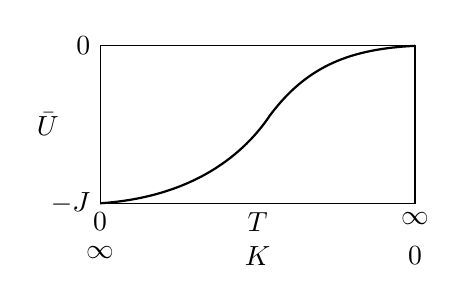
\begin{tikzpicture}[scale=0.8]
  \draw (0,0) rectangle (5,2.5);
  \draw[thick] (0,0) .. controls (1.5,0.1) and (2.3,0.8) .. (2.7,1.4) .. controls (3.3,2.2) and (4,2.45) .. (5,2.5);
  \node[left] at (0,2.5) {$0$}; \node[left] at (0,0) {$-J$};
  \node[left] at (-0.5,1.25) {$\bar U$};
  \node[below] at (0,0) {$0$}; \node[below] at (5,0) {$\infty$}; \node[below] at (2.5,0) {$T$};
  \node[below=12pt] at (0,0) {$\infty$}; \node[below=12pt] at (5,0) {$0$}; \node[below=12pt] at (2.5,0) {$K$};
\end{tikzpicture}
\diagramcaption{Internal energy per site of the 1D Ising ferromagnet.}
\end{diagram}

% Source: Lecture6.pdf, pages 1-7 (page 8 is blank).
\lecture{6}
\paragraph{1D Ising model, continued.}

Recall: with PBC,
$Z = \sum_{\{\sigma_i\}}e^{-\beta\Ham} = \Tr(T^N)$, where $T$ = transfer matrix, with
matrix elements
\begin{equation}
  \langle\sigma_{i+1}|T|\sigma_i\rangle = e^{K\sigma_{i+1}\sigma_i+(h/2)(\sigma_{i+1}+\sigma_i)},
  \qquad K\equiv\beta J,\quad h\equiv\beta H,
  \qquad
  T = \begin{pmatrix} e^{K+h} & e^{-K}\\ e^{-K} & e^{K-h}\end{pmatrix}.
\end{equation}
For $H = 0$, the eigenvalues of $T$ are $\lambda_+ = 2\cosh K$, $\lambda_- = 2\sinh K$. So
\begin{equation}
  Z = \Tr(T^N) = \lambda_+^N + \lambda_-^N = 2^N(\cosh K)^N[1+v^N],\qquad v = \tanh K .
\end{equation}
The Gibbs free energy per site is $\bar G(T,H) = -\kB Tf$, where $f$ = the dimensionless
reduced free energy. We will usually take the thermodynamic limit $N\to\infty$, with
\begin{equation}
  f = \lim_{N\to\infty}\frac{1}{N}\ln Z = \ln[2\cosh K] = \ln(\lambda_+).
\end{equation}
This illustrates that $f$ and the resultant thermodynamic functions are determined by the
dominant (= maximal) eigenvalue of the transfer matrix. This is $\lambda_+$ since
$\cosh K>\sinh K$. The internal energy per site is
\begin{equation}
  \bar U = -\pder{f}{\beta} = -J\pder{f}{K} = -J\tanh K = -J\tanh(\beta J).
\end{equation}
N.B.: this is invariant under $J\to -J$.

\subsubsection*{Ferromagnet--antiferromagnet mapping on bipartite lattices}

\paragraph{Theorem.} On a bipartite lattice,
$\Lambda = \Lambda_e\oplus\Lambda_o$, there is a mapping that relates a spin model with the
FM sign of $J$, $J>0$, to the model with the AFM sign of $J$, $J<0$, if the external field
$H = 0$. The mapping is
\begin{equation}
  J\to -J,\qquad
  \sigma_i\to\sigma_i\ \text{if } i\in\Lambda_e,\qquad
  \sigma_i\to-\sigma_i\ \text{if } i\in\Lambda_o .
\end{equation}
Then
$\Ham = -J\sum_{\langle ij\rangle}\sigma_i\sigma_j\to-(-J)\sum_{\langle ij\rangle}(-\sigma_i\sigma_j)$
is invariant, since all of the nearest neighbors of a site $i\in\Lambda_{\text{even}}$ are
in $\Lambda_{\text{odd}}$.

\begin{diagram}
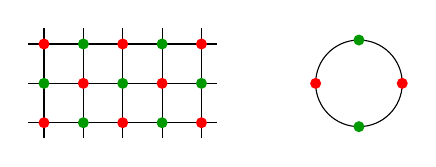
\begin{tikzpicture}[scale=0.5]
  \foreach \x in {0,...,4} \draw (\x,-0.4) -- (\x,2.4);
  \foreach \y in {0,1,2} \draw (-0.4,\y) -- (4.4,\y);
  \foreach \x in {0,...,4} \foreach \y in {0,1,2} {
    \pgfmathtruncatemacro{\prty}{mod(\x+\y,2)}
    \ifnum\prty=0 \fill[red] (\x,\y) circle (0.14); \else \fill[green!60!black] (\x,\y) circle (0.14); \fi}
  \begin{scope}[xshift=8cm,yshift=1cm]
    \draw (0,0) circle (1.1);
    \fill[green!60!black] (0,1.1) circle (0.14); \fill[green!60!black] (0,-1.1) circle (0.14);
    \fill[red] (1.1,0) circle (0.14); \fill[red] (-1.1,0) circle (0.14);
  \end{scope}
\end{tikzpicture}
\diagramcaption{Bipartite lattices: each red site has nearest neighbors that are green,
and vice versa. Left: the square lattice. Right: a 1D ring with an even number of sites.}
\end{diagram}

Our 1D lattice is bipartite iff $N$ is even, and we can take the limit $N\to\infty$ on even
values. The interaction Hamiltonian is invariant under this mapping, and so is the sum
$\sum_{\{\sigma_i\}}e^{-\beta\Ham}$, since each $\sigma_i$ takes on $\pm 1$ values. So for the
$H = 0$ case we can, with no loss of generality, take $J>0$:
\begin{equation}
  \bar U = -J\ev{\sigma_2\sigma_1} = -J\tanh(\beta J).
\end{equation}
As $T\to\infty$, $\beta\to 0$, the spins are random, so $\ev{\sigma_2\sigma_1}\to 0$. As
$T\to 0$, the FM coupling favors short-range order; $\tanh(\beta J)\to 1$ as $\beta\to\infty$.
(See the plot of $\bar U$ at the end of the previous lecture.)

\subsubsection*{Specific heat of the 1D Ising model}

Next, calculate the specific heat (per spin), $\bar C = \left.\dd\bar U/\dd T\right|_{H=0}$;
we drop the bars in the notation henceforth. Now
$K = \beta J = J/(\kB T)$, i.e.\ $T = J/(\kB K)$, so $\dd T = -(J/(\kB K^2))\dd K$, i.e.\
$\dd K/\dd T = -\kB K^2/J$. With $U = -\partial f/\partial \beta = -J\partial f/\partial K$,
\begin{equation}
  C = \pder{U}{T} = \pder{K}{T}\cdot\pder{U}{K}
    = \left(-\frac{\kB K^2}{J}\right)\pder{U}{K}
    = -\left(\frac{\kB K^2}{J}\right)\pder{}{K}\left(-J\pder{f}{K}\right)
    = \kB K^2\frac{\partial^2 f}{\partial K^2}.
\end{equation}
($C$ is the second derivative of $f$ with respect to $T$, or equivalently $K$.) Since
$(\dd/\dd K)\tanh K = 1/(\cosh^2K)$,
\begin{equation}
  C = \left(-\frac{\kB K^2}{J}\right)\left(-\frac{J}{\cosh^2K}\right) = \frac{\kB K^2}{\cosh^2K}.
\end{equation}
Now $\cosh K = (e^K+e^{-K})/2$, so as
\begin{equation}
  \begin{cases}
    T\to\infty,\ \text{i.e.}\ \beta\to 0,\ K\to 0: & \cosh K\to 1,\\[6pt]
    T\to 0,\ \text{i.e.}\ \beta\to\infty,\ K\to\infty: & \cosh K\sim\dfrac{e^K}{2}.
  \end{cases}
\end{equation}
So as $T\to 0$, $C\to 4\kB K^2e^{-2K}\propto 4\kB T^{-2}e^{-2J/T}$, an essential zero; as
$T\to\infty$, $C\to\kB K^2\propto T^{-2}$, which vanishes as a power of $T$.

\begin{diagram}
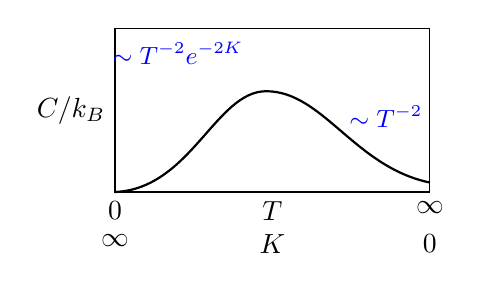
\begin{tikzpicture}[scale=0.8]
  \draw (0,0) rectangle (5,2.6);
  \draw[thick] (0,0) .. controls (1.2,0.05) and (1.6,1.6) .. (2.4,1.6) .. controls (3.3,1.6) and (3.8,0.4) .. (5,0.15);
  \node[left] at (0,1.3) {$C/\kB$};
  \node[below] at (0,0) {$0$}; \node[below] at (5,0) {$\infty$}; \node[below] at (2.5,0) {$T$};
  \node[below=12pt] at (0,0) {$\infty$}; \node[below=12pt] at (5,0) {$0$}; \node[below=12pt] at (2.5,0) {$K$};
  \node[blue,font=\small] at (1,2.2) {$\sim T^{-2}e^{-2K}$};
  \node[blue,font=\small] at (4.3,1.2) {$\sim T^{-2}$};
\end{tikzpicture}
\diagramcaption{Schematic graph of the specific heat of the 1D Ising model.}
\end{diagram}

This behavior can be understood physically: the specific heat $C$ measures how the internal
energy changes as one changes the temperature $T$. As $T\to 0$, the spins are approaching a
frozen state $+++++$ or $-----$, and $U$ approaches $-J$, so taking $T\to 0.1\,T$ has almost
no effect, so $C\to 0$. As $T\to\infty$, the spins are almost completely random, and
$U\to 0$, so taking $T\to 10\,T$ has a negligible effect on $U$ and hence again, $C\to 0$. The
specific heat reaches a max at an intermediate temperature $T$ such that $\kB T\sim J$, since
for temperatures of this order a change in $T$ has a significant effect on the local spin
order and hence on $U$.

\subsection{The 1D Ising model in a magnetic field}
\subsubsection*{Nonzero external field}

Next, apply a nonzero external magnetic field $H$. Calculate the eigenvalues of the transfer
matrix $T$. Recall
$T = \left(\begin{smallmatrix} e^{K+h} & e^{-K}\\ e^{-K} & e^{K-h}\end{smallmatrix}\right)$.
The indicial equation for the eigenvalues is
\begin{gather}
  (e^{K+h}-\lambda)(e^{K-h}-\lambda) - e^{-2K} = 0\nonumber\\
  \Rightarrow\ \lambda^2 - (e^{K+h}+e^{K-h})\lambda + (e^{2K}-e^{-2K}) = 0
  \ \Rightarrow\ \lambda^2 - e^K\,2\cosh h\,\lambda + 2\sinh(2K) = 0,
\end{gather}
so
\begin{align}
  \lambda_\pm &= \frac{1}{2}\left[2e^K\cosh h\pm\sqrt{4e^{2K}\cosh^2h - 8\sinh(2K)}\right]\nonumber\\
  &= e^K\left[\cosh h\pm\sqrt{\cosh^2h - 2e^{-2K}\sinh(2K)}\right]\nonumber\\
  &= e^K\left[\cosh h\pm\sqrt{\left(\frac{e^h+e^{-h}}{2}\right)^2 - 2e^{-2K}\left(\frac{e^{2K}-e^{-2K}}{2}\right)}\right]\nonumber\\
  &= e^K\left[\cosh h\pm\sqrt{\frac{1}{4}(e^{2h}+2+e^{-2h}) + (-1+e^{-4K})}\right].
\end{align}
Since $(1/4)(e^{2h}+2-4+e^{-2h}) = (\sinh h)^2$, an equivalent expression for $\lambda_\pm$
is
\begin{equation}
  \lambda_\pm = e^K\left[\cosh h\pm\sqrt{(\sinh h)^2+e^{-4K}}\right],\qquad h = \beta H .
\end{equation}
Here $\lambda_+$ is the maximal eigenvalue of $T$, and $f = \ln\lambda_+$,
$\bar G(T,H) = -\kB Tf = -\beta^{-1}f$.

\paragraph{Magnetization.}

Now calculate the induced magnetization per site:
\begin{equation}
  \bar M = \lim_{N\to\infty}\frac{1}{N}\left[\frac{\sum_{\{\sigma_i\}}\left(\sum_j\sigma_j\right)e^{-\beta\Ham}}{\sum_{\{\sigma_i\}}e^{-\beta\Ham}}\right]
  = \left(\pder{f}{h}\right)_T = \frac{1}{\beta}\left(\pder{f}{H}\right)_T = -\left(\pder{\bar G}{H}\right)_T ;
\end{equation}
recall $\dd G(T,H) = -S\dd T - M\dd H$, so $M = -(\partial G/\partial H)_T$. So
\begin{equation}
  \bar M = \pder{\ln\lambda_+}{h} = \frac{1}{\lambda_+}\pder{\lambda_+}{h};
  \qquad\text{define}\quad \tilde\lambda_+ = e^{-K}\lambda_+ .
\end{equation}
Now
\begin{equation}
  \pder{\tilde\lambda_+}{h} = \sinh h + \frac{1}{2}\cdot\frac{2(\sinh h)(\cosh h)}{\sqrt{\sinh^2h+e^{-4K}}}
  = (\sinh h)\left[1 + \frac{\cosh h}{\sqrt{\sinh^2h+e^{-4K}}}\right],
\end{equation}
\begin{equation}
  \frac{1}{\lambda_+}\pder{\lambda_+}{h} = \frac{1}{\tilde\lambda_+}\pder{\tilde\lambda_+}{h}
  = \frac{(\sinh h)\left[\frac{\sqrt{\sinh^2h+e^{-4K}}+\cosh h}{\sqrt{\sinh^2h+e^{-4K}}}\right]}{\cosh h+\sqrt{\sinh^2h+e^{-4K}}}
  = \frac{\sinh h}{\sqrt{\sinh^2h+e^{-4K}}},
\end{equation}
so
\begin{equation}
  \boxed{\bar M = \frac{\sinh h}{\sqrt{\sinh^2h+e^{-4K}}}}\,;
  \qquad\text{spontaneous magnetization}\quad \bar M_{\text{spont.}} = \lim_{h\to 0}\bar M .
\end{equation}
For any temperature $T>0$, hence finite $K = \beta J$, this limit $=0$:
$\bar M_{sp} = 0\ \forall\, T>0$. If we set $T = 0$, i.e.\ $\beta = \infty$, $K = \infty$, then
$e^{-4K} = 0$, so $|\bar M| = 1$ ($\bar M = \sgn(H)$). So
\begin{equation}
  |\bar M| = \begin{cases} 0 & \forall\, T>0\\ 1 & \text{for } T = 0.\end{cases}
\end{equation}
$\bar M_{sp}$ thus has a discontinuous behavior as $T\to 0$.

\begin{diagram}
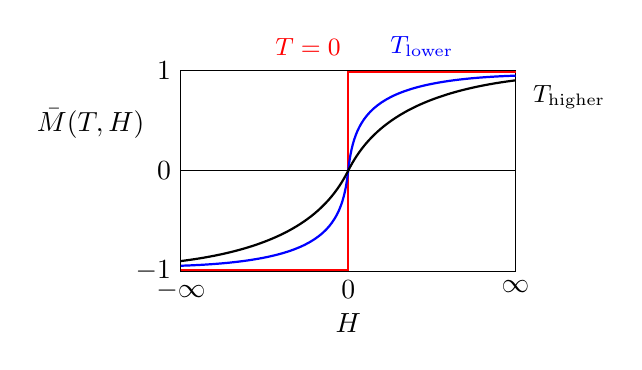
\begin{tikzpicture}[scale=0.85]
  \draw (0,0) rectangle (5,3);
  \draw (0,1.5) -- (5,1.5); \draw (2.5,0) -- (2.5,3);
  \draw[thick,red] (0,0.02) -- (2.5,0.02) -- (2.5,2.98) -- (5,2.98);
  \draw[thick,blue] (0,0.08) .. controls (2.1,0.15) and (2.4,0.6) .. (2.5,1.5) .. controls (2.6,2.4) and (2.9,2.85) .. (5,2.92);
  \draw[thick] (0,0.15) .. controls (1.6,0.35) and (2.2,0.9) .. (2.5,1.5) .. controls (2.8,2.1) and (3.4,2.65) .. (5,2.85);
  \node[left] at (0,3) {$1$}; \node[left] at (0,1.5) {$0$}; \node[left] at (0,0) {$-1$};
  \node[left] at (-0.4,2.2) {$\bar M(T,H)$};
  \node[below] at (0,0) {$-\infty$}; \node[below] at (2.5,0) {$0$}; \node[below] at (5,0) {$\infty$};
  \node[below=12pt] at (2.5,0) {$H$};
  \node[red,font=\small] at (1.9,3.35) {$T=0$};
  \node[blue,font=\small] at (3.6,3.35) {$T_{\text{lower}}$};
  \node[font=\small] at (5.8,2.6) {$T_{\text{higher}}$};
\end{tikzpicture}
\diagramcaption{Magnetization of the 1D Ising model, taking account of the reversal in
$\sgn(\bar M)$ with $\sgn(H)$.}
\end{diagram}

\subsubsection*{The Peierls theorem in one dimension}

The fact that there is no spontaneous magnetization, i.e.\ no ``long-range order'' (LRO), at
any finite temperature in this model is a consequence of a general theorem, the (1D form of
the) \emph{Peierls theorem}: given a spin system with finite-range interactions (e.g.\
nearest-neighbor interactions), there is no LRO = spontaneous magnetization at any $T>0$.

\paragraph{Proof.} The equilibrium state is obtained by minimizing the free energy. Consider
$A = U - TS$ (or $G = U - TS - HM$, with $H = 0$). Consider a hypothetical ordered state
$+++++\cdots$ and show that it is unstable to the appearance of a seam (for FBC) with reversal
of spins: $+++++\,|\,-----$. The change in $\Delta A$ or $\Delta G$ is
\begin{equation}
  \Delta G = +2J - T\ln N,
\end{equation}
where the bond energy changes from $-J$ ($++$) to $+J$ ($+-$), a difference of $2J$, and
$-T\Delta S = -T\ln N$ since the seam can occur at any of the $N$ sites on the lattice. So
for any $T>0$, as $N\to\infty$, the entropy term dominates and $\Delta G<0$, so the disordering
seams are preferred over the hypothetical ordered state. Only at $T = 0$ is the entropy term
absent; then $\Delta G = \Delta U$ and the appearance of the seam is dispreferred. That is,
if and only if $T = 0$, then the minimization of the free energy is the same as the
minimization of the internal energy.

\subsubsection*{Susceptibility}

Next, calculate the (isothermal) magnetic susceptibility $\chi = (\partial M/\partial H)_T$
and, per site,
\begin{equation}
  \bar\chi = \left(\pder{\bar M}{H}\right)_T = \beta\left(\pder{\bar M}{h}\right)_T
  = \beta\left(\frac{\partial^2 f}{\partial h^2}\right)_T .
\end{equation}
As is evident, $\chi$ is a second derivative of $f$ with respect to $h$. Now
\begin{align}
  \pder{\bar M}{h} &= \pder{}{h}\left[\frac{\sinh h}{\sqrt{\sinh^2h+e^{-4K}}}\right]\nonumber\\
  &= \frac{\cosh h}{\sqrt{\sinh^2h+e^{-4K}}}
    - \frac{1}{2}(\sinh h)(\sinh^2h+e^{-4K})^{-3/2}\cdot(2\sinh h\cosh h)\nonumber\\
  &= \frac{\cosh h}{\sqrt{\sinh^2h+e^{-4K}}}\left[1-\frac{\sinh^2h}{\sinh^2h+e^{-4K}}\right]
   = \frac{e^{-4K}\cosh h}{(\sinh^2h+e^{-4K})^{3/2}},
\end{align}
so
\begin{equation}
  \bar\chi = \frac{\beta e^{-4K}\cosh h}{(\sinh^2h+e^{-4K})^{3/2}};
  \qquad\text{zero-field susceptibility:}\quad \bar\chi_{H=0} = \beta e^{2K}.
\end{equation}
$\bar\chi_{H=0}$ diverges exponentially as $T\to 0$, i.e.\ $K\to\infty$ (an essential divergence
$\sim e^{2J/T}$ as a function of $T$). So the 1D Ising model has a (1-sided) phase transition at
$T = 0$. Rather than algebraic singularities, it has a combination of essential singularities in
$\bar C$ and $\bar\chi_{H=0}$ and a discontinuous singularity in
$M_{H=0} = M_{\text{spontaneous}}$.

\subsection{Correlations in the 1D Ising model}
\subsubsection*{Spin--spin correlation function by a high-temperature expansion}

Calculate the spin--spin correlation function
$\ev{\sigma_i\sigma_j}_{H=0} = \ev{\sigma_i\sigma_j}_{\text{conn.},H=0}$, where $i$, $j$ are
arbitrary. The method is a high-temperature series expansion. Here
\begin{equation}
  \ev{\sigma_i\sigma_j}_{\text{conn}}\equiv\ev{\sigma_i\sigma_j}-\ev{\sigma}^2 = \ev{\sigma_i\sigma_j}-\bar M^2 .
\end{equation}
Consider $T>0$; here $\bar M = 0$, so $\ev{\sigma_i\sigma_j} = \ev{\sigma_i\sigma_j}_{\text{connected}}$.
With $\langle ij\rangle$ the nearest neighbors (n.n.),
\begin{equation}
  Z = \sum_{\{\sigma_i\}}e^{-\beta\Ham} = \sum_{\{\sigma_i\}}e^{K\sum_{\langle ij\rangle}\sigma_i\sigma_j}
    = \sum_{\{\sigma_i\}}\left[\prod_{\langle ij\rangle}e^{K\sigma_i\sigma_j}\right].
\end{equation}
Use $e^x = \sum_{n=0}^\infty x^n/n!$ and $\sigma_i = \pm 1$, $\sigma_i^2 = 1$:
\begin{align}
  e^{K\sigma_i\sigma_j} &= 1 + K\sigma_i\sigma_j + \frac{1}{2!}(K\sigma_i\sigma_j)^2
     + \frac{1}{3!}(K\sigma_i\sigma_j)^3 + \frac{1}{4!}K^4 + \frac{1}{5!}K^5\sigma_i\sigma_j+\cdots\nonumber\\
  &= \underbrace{\left[1+\frac{K^2}{2!}+\frac{K^4}{4!}+\cdots\right]}_{\cosh K}
   + \sigma_i\sigma_j\underbrace{\left[K+\frac{K^3}{3!}+\frac{K^5}{5!}+\cdots\right]}_{\sinh K}
\end{align}
(recall $\cosh x = 1 + x^2/2!+x^4/4!+\cdots$ and
$\sinh x = x + x^3/3!+x^5/5!+\cdots$), so
\begin{equation}
  e^{K\sigma_i\sigma_j} = \cosh K + \sigma_i\sigma_j\sinh K = \cosh K\,(1+v\sigma_i\sigma_j),
  \qquad v\equiv\tanh K .
\end{equation}
This is an identity; $|v|\to 0$ as $T\to\infty$. Therefore
\begin{equation}
  Z = \sum_{\{\sigma_i\}}\left[\prod_{\langle ij\rangle}e^{K\sigma_i\sigma_j}\right]
    = \sum_{\{\sigma_i\}}\prod_{\langle ij\rangle}\cosh K\,(1+v\sigma_i\sigma_j)
    = (\cosh K)^{e(\Lambda)}\sum_{\{\sigma_i\}}\left[\prod_{\langle ij\rangle}(1+v\sigma_i\sigma_j)\right],
\end{equation}
since to each n.n.\ pair $\langle ij\rangle$ there is a bond. For a lattice $\Lambda$ with
coordination number $\Delta\equiv$ degree of each site in $\Lambda$,
\begin{equation}
  e(\Lambda) = \frac{\Delta}{2}n(\Lambda),
\end{equation}
so $e(\Lambda_{1D}) = n$ for a 1D lattice with PBC, and
\begin{equation}
  Z = (\cosh K)^{(\Delta/2)n}\sum_{\{\sigma_i\}}\left[\prod_{\langle ij\rangle}(1+v\sigma_i\sigma_j)\right].
\end{equation}

\paragraph{Example: a triangle.} Illustrate this with a calculation of $Z$ for a (finite)
$\Lambda$, the triangle with vertices 1, 2, 3:
\begin{align}
  Z &= (\cosh K)^3\sum_{\{\sigma_i\}}(1+v\sigma_1\sigma_2)(1+v\sigma_2\sigma_3)(1+v\sigma_3\sigma_1)\nonumber\\
    &= (\cosh K)^3\sum_{\{\sigma_i\}}\left[1 + v(\sigma_1\sigma_2+\sigma_2\sigma_3+\sigma_3\sigma_1)
       + v^2(\sigma_1\sigma_2\sigma_2\sigma_3+\text{cycl.}) + v^3\sigma_1\sigma_2\sigma_2\sigma_3\sigma_3\sigma_1\right]\nonumber\\
    &= (\cosh K)^3(1+v^3)\cdot 2^3 ,
\end{align}
since the terms linear in $v$ and the terms $v^2\sigma_1\sigma_3$ etc.\ sum to zero. So for this
illustrative example with $N = 3$,
\begin{equation}
  Z = (2^3)(\cosh K)^3(1+v^3) = (2\cosh K)^3 + (2\sinh K)^3 = \lambda_+^N+\lambda_-^N\quad\text{with } N = 3 .
\end{equation}
This shows how this expansion yields $Z$ and shows the method (series in powers of $K$, or
equivalently $v$) used in high-temperature series.

\paragraph{Correlation function.} Now use this method to calculate $\ev{\sigma_n\sigma_{n'}}$.
Note that, due to the homogeneity of $\Lambda$ (with PBC), this 2-spin correlation function
only depends on $|n-n'|$. E.g.\ calculate $\ev{\sigma_0\sigma_2}$ on a ring of sites
$0,1,2,3$:
\begin{equation}
  \ev{\sigma_0\sigma_2} = \frac{\sum_{\{\sigma_i\}}\sigma_0\sigma_2e^{-\beta\Ham}}{\sum_{\{\sigma_i\}}e^{-\beta\Ham}}
  = \frac{\sum_{\{\sigma_i\}}\sigma_0\sigma_2\prod_{\langle ij\rangle}(1+v\sigma_i\sigma_j)}{\sum_{\{\sigma_i\}}\prod_{\langle ij\rangle}(1+v\sigma_i\sigma_j)}.
\end{equation}
The numerator is
\begin{align}
  &\sum_{\{\sigma_i\}}\sigma_0\sigma_2(1+v\sigma_0\sigma_1)(1+v\sigma_1\sigma_2)(1+v\sigma_2\sigma_3)(1+v\sigma_3\sigma_0)\nonumber\\
  &\quad= \sum_{\{\sigma_i\}}\sigma_0\sigma_2\left[1 + v(\sigma_0\sigma_1+\text{cycl.}) + v^2(\sigma_0\sigma_1\cdot\sigma_1\sigma_2+\cdots)+\cdots\right]
  \ \propto\ v^2 + v^{N-2}
\end{align}
(any unmatched $\sigma_i$ gives zero after the sum). Now generalize this; by a similar method,
\begin{equation}
  \ev{\sigma_0\sigma_\ell} = v^\ell + v^{N-\ell}.
\end{equation}
Next, take the thermodynamic limit $N\to\infty$. For our $T>0$ regime, $|v|<1$, so
$\lim_{N\to\infty}v^{N-\ell} = 0$ and hence
\begin{equation}
  \boxed{\ev{\sigma_0\sigma_\ell} = v^\ell},\qquad v = \tanh K .
\end{equation}
This completes the calculation of the 2-spin correlation function in the 1D Ising model
(for $H = 0$).

% Source: Lecture7.pdf, pages 1-3 (1D Ising model, continued). Page 8 is blank.
% The Potts-model half of the lecture (pages 3-7) is in lec07-potts.tex.
\lecture{7}
\subsubsection*{Correlation length and susceptibility of the 1D Ising model}

Previously, we calculated (for $H = 0$) the 2-spin correlation function
\begin{equation}
  \ev{\sigma_0\sigma_\ell} = v^\ell,\qquad \ell\ge 0,
\end{equation}
where $v = \tanh K$, $K = \beta J$. Recall that for $T>0$, since $|\tanh K|<1$,
\begin{enumerate}[label=(\arabic*)]
  \item $|\ev{\sigma_0\sigma_\ell}|$ is a monotonically decreasing function of $\ell\ge 0$, where $\ell$ is the distance
    between the spins in lattice units (if $\ell = 0$, $\ev{\sigma_0^2} = 1$);
  \item for fixed $\ell\ge 1$, $|\ev{\sigma_0\sigma_\ell}|$ is a monotonically decreasing function of $T$.
\end{enumerate}
These properties are physically understandable. Property (1) expresses the fact that as the two spins get farther and
farther apart, the value of spin $\sigma_0$ has a progressively smaller and smaller influence on the value of spin
$\sigma_\ell$. Property (2) follows because the higher the temperature $T$ is, i.e.\ the smaller $\beta$ and $|K|$ are, the
less is the ordering effect of the interaction term in $e^{-\beta\Ham} = e^{K\sum_{\langle ij\rangle}\sigma_i\sigma_j}$.

Also, note that the property that $\tanh(K)$ is an odd function of $K$ means that this correlation function has the
properties expected from the ferromagnetic (FM) and antiferromagnetic (AFM) signs of the spin--spin coupling, respectively
$J>0$ and $J<0$, namely that $\ev{\sigma_0\sigma_\ell}>0$ for FM $J$, while for AFM $J<0$,
\begin{equation}
  \ev{\sigma_0\sigma_\ell} = (\tanh K)^\ell = (-1)^\ell|\tanh K|^\ell
  = \begin{cases} >0 & \text{if $\ell$ even}\\ <0 & \text{if $\ell$ odd.}\end{cases}
\end{equation}
\begin{equation*}
  \text{FM order:}\quad
  \begin{array}{cccc} + & + & + & +\\[-2pt] \scriptstyle 0 & \scriptstyle 1 & \scriptstyle 2 & \scriptstyle 3\end{array}
  \ \text{or}\
  \begin{array}{cccc} - & - & - & -\\[-2pt] \scriptstyle 0 & \scriptstyle 1 & \scriptstyle 2 & \scriptstyle 3\end{array}
  \qquad\qquad
  \text{AFM order:}\quad
  \begin{array}{cccc} + & - & + & -\\[-2pt] \scriptstyle 0 & \scriptstyle 1 & \scriptstyle 2 & \scriptstyle 3\end{array}
  \ \text{or}\
  \begin{array}{cccc} - & + & - & +\\[-2pt] \scriptstyle 0 & \scriptstyle 1 & \scriptstyle 2 & \scriptstyle 3\end{array}
\end{equation*}

\paragraph{Correlation length.}

Next, calculate the correlation length $\xi$. Because of the bipartite nature of the 1D lattice, we may take $J>0$ with no
loss of generality. Recall that for $T\ne T_c$, a connected correlation function decays exponentially as the distance
between the spins gets large; $\ev{\sigma_0\sigma_r}\sim e^{-r/\xi}$ (in higher dimensions there may be power-law
prefactors, but here these are absent). So we have (with $v = \tanh K$)
\begin{equation}
  v^r = e^{-r/\xi}\ \Rightarrow\ v = e^{-1/\xi}\ \Rightarrow\ \ln v = -\frac{1}{\xi},\quad\text{i.e.}\quad
  \xi = -\frac{1}{\ln v} = \frac{1}{\ln\left(1/v\right)} .
\end{equation}
Since $v$ decreases with increasing $T$, $\ln(1/v)$ increases, and $\xi$ decreases. Again, this makes sense physically; as
$T$ increases, there is greater thermal disorder, so the correlation length should decrease.

Next, calculate the singularity in $\xi$ as $T\to 0$, i.e.\ $K\to\infty$:
\begin{align}
  \xi &= \frac{1}{\ln\left(1/v\right)};\qquad
  \frac{1}{v} = \frac{1}{\tanh K} = \frac{\cosh K}{\sinh K} = \frac{e^K+e^{-K}}{e^K-e^{-K}} = \frac{1+e^{-2K}}{1-e^{-2K}}\nonumber\\
  &\simeq\left(1+e^{-2K}\right)\left(1+e^{-2K}+\cdots\right) = 1+2e^{-2K},
\end{align}
so
\begin{equation}
  \ln\left(\frac{1}{v}\right)\simeq\ln\left(1+2e^{-2K}\right)\simeq 2e^{-2K}\ \Rightarrow\
  \xi\simeq\frac{1}{2e^{-2K}} = \frac{1}{2}e^{2K}\quad\text{as } T\to 0 .
\end{equation}
So the correlation length $\xi$ diverges exponentially rapidly as $T\to 0$,
\begin{equation}
  \xi\simeq\frac{1}{2}e^{2J/(\kB T)},
\end{equation}
an essential singularity. This is similar to what we found for $\bar\chi$, the initial ($H = 0$) magnetic susceptibility,
$\bar\chi_{H=0} = \beta e^{2K}$.

\paragraph{Susceptibility from the correlation function.}

It is useful to exhibit a different way to calculate $\bar\chi_{H=0}$. To do this we recall that, just as
$\bar M = \partial f/\partial h$ ``pulls down'' one $\sigma_i$ from $e^{-\beta\Ham}$,
\begin{equation}
  \bar M = \lim_{N\to\infty}\frac{1}{N}\,\frac{\sum_{\{\sigma_i\}}\left(\sum_j\sigma_j\right)e^{-\beta\Ham}}{\sum_{\{\sigma_i\}}e^{-\beta\Ham}},
\end{equation}
the susceptibility
\begin{equation}
  \bar\chi = \pder{\bar M}{H} = \beta\pder{\bar M}{h} = \beta\frac{\partial^2f}{\partial h^2}
\end{equation}
``pulls down'' two $\sigma$'s. For $T>0$, $\ev\sigma = \bar M = 0$, and
\begin{equation}
  \beta^{-1}\bar\chi = \lim_{N\to\infty}\frac{1}{N}\sum_{\text{all }i,j}\ev{\sigma_i\sigma_j},
\end{equation}
where, as indicated, $i$ and $j$ range over all sites. Since the lattice is homogeneous, this
$\lim_{N\to\infty}\sum_{i,j}$ double sum is equal to the sum over one site with the other fixed:
\begin{equation}
  \lim_{N\to\infty}\frac{1}{N}\sum_{\text{all }i,j}\ev{\sigma_i\sigma_j} = \sum_j\ev{\sigma_0\sigma_j},\qquad j\in\mathbb Z .
\end{equation}
Further, $\ev{\sigma_0\sigma_j} = \ev{\sigma_0\sigma_{-j}} = v^{|j|}$. So
\begin{equation}
  \sum_{j\in\mathbb Z}\ev{\sigma_0\sigma_j} = \underbrace{\ev{\sigma_0\sigma_0}}_{1}
  + \sum_{j=-\infty}^{-1}\ev{\sigma_0\sigma_j} + \sum_{j=1}^\infty\ev{\sigma_0\sigma_j}
  = 1 + 2\sum_{j=1}^\infty\ev{\sigma_0\sigma_j} = 1 + 2\sum_{j=1}^\infty v^j .
\end{equation}
Now $\sum_{j=0}^\infty v^j = 1/(1-v)$, provided this series converges, which it does for $|v|<1$, so
\begin{equation}
  \sum_{j=1}^\infty v^j = -v^0 + v^0 + \sum_{j=1}^\infty v^j = -1 + \sum_{j=0}^\infty v^j = -1 + \frac{1}{1-v} = \frac{v}{1-v}.
\end{equation}
So $1 + 2\sum_{j=1}^\infty v^j = 1 + 2\left(v/(1-v)\right) = (1+v)/(1-v)$, so
\begin{align}
  \beta^{-1}\bar\chi &= \frac{1+v}{1-v} = \frac{1+\tanh K}{1-\tanh K} = \frac{\cosh K+\sinh K}{\cosh K-\sinh K}\nonumber\\
  &= \frac{\left(e^K+e^{-K}\right)+\left(e^K-e^{-K}\right)}{\left(e^K+e^{-K}\right)-\left(e^K-e^{-K}\right)} = \frac{2e^K}{2e^{-K}} = e^{2K},
\end{align}
i.e.\ $\bar\chi = \beta e^{2K}$, as we derived earlier.

\paragraph{Susceptibility in a nonzero field.}

Next, discuss our earlier result in the case of a nonzero external magnetic field $H$. Recall the expression
\begin{equation}
  \bar\chi = \frac{\beta e^{-4K}\cosh h}{\left[\sinh^2h+e^{-4K}\right]^{3/2}}.
\end{equation}
Consider the behavior as $T\to\infty$, i.e.\ $\beta\to 0$, $K\to 0$ and $h\equiv\beta H\to 0$, so $\sinh h\to 0$,
$e^{-4K}\to 1$, $\cosh h\to 1$, $\bar\chi\to\beta$. This is the realization, in this model, of the Curie (Pierre Curie)
``law'', that $\bar\chi\propto\beta\propto1/T$ at high temperature $T$. This is observed experimentally in 3D as well as
lower-dimensional substances.

Consider the behavior as $T\to 0$. Here, with $H\ne 0$, one must analyze the $J>0$ (FM) and $J<0$ (AFM) cases separately.
This is clear, since an external magnetic field $H$ biases the system toward FM spin ordering ($h = \beta H$).
\begin{enumerate}[label=(\arabic*)]
  \item Case $J>0$: here, as $T\to 0$, $K\to\infty$ so $e^{-4K}\to 0$, and $h\to\infty$:
    $\cosh h\to e^h/2$, $\sinh h\to e^h/2$, $\cosh h/(\sinh^3h)\to(e^h/2)/(e^h/2)^3 = 4e^{-2h}$, so
    \begin{equation}
      \bar\chi\to\frac{\beta e^{-4K}\cosh h}{\sinh^3h}\to 4\beta e^{-4K}e^{-2h}\to 0 .
    \end{equation}
    This vanishing of $\bar\chi$ for $H\ne 0$ is physically understandable, because the external magnetic field biases the
    spins toward FM order, and this approaches a complete ordering as $T\to 0$, $|\bar M|\to 1$, so increasing $H$ has a
    negligible effect and $\bar\chi = \partial \bar M/\partial H\to 0$.
  \item Case $J<0$: here one has competing interactions: (i) the spin--spin interaction prefers the spins to order
    antiferromagnetically: $+-+-+-$; (ii) the external magnetic field prefers the spins to order ferromagnetically. This is
    an exactly solvable example of competing interactions. Which one dominates over the other? This will be a homework
    problem.
\end{enumerate}

\section{Potts models and graph theory}
% Source: Lecture7.pdf, pages 3-7 (the Potts model).
\subsection{The Potts model and its solution in one dimension}
\subsubsection*{From the Ising model to the Potts model}

Next, discuss a generalization of the Ising model. The dynamical variables in the Ising model take on 2 values,
$\sigma_i = \pm1$. The spin--spin interaction (with $H = 0$)
\begin{equation}
  \Ham_{\text{int.}}^{(I)} = -J_I\sum_{\langle ij\rangle_{\text{n.n.}}}\sigma_i\sigma_j
\end{equation}
also takes on 2 values: $-J_I$ for the pairs $++$, $--$, and $+J_I$ for the pairs $+-$, $-+$; the difference is $2|J_I|$,
where we use a superscript or subscript $I$ to denote Ising.

This is equivalent to a model in which the dynamical variables $\sigma_i$ take on the values 1 or 2 and the spin--spin
interaction involves a Kronecker $\delta_{\sigma_i\sigma_j}$:
\begin{equation}
  \Ham_{\text{int.}}^{(P)} = -J_P\sum_{\langle ij\rangle_{\text{n.n.}}}\delta_{\sigma_i\sigma_j}\qquad(H = 0),
\end{equation}
with $\Ham_{\text{int.}} = -J_P$ for the pairs $11$, $22$ and $\Ham_{\text{int.}} = 0$ for the pairs $12$, $21$; the difference
is $|J_P|$. If $J>0$, $\Ham_{\text{int.}}$ prefers $\sigma_i$ and $\sigma_j$ to have the same value. If $J<0$,
$\Ham_{\text{int.}}$ prefers $\sigma_i$ and $\sigma_j$ to have different values. These formulations are equivalent if we set
$2J_I = J_P$ and shift the zero of the energy by a constant. This constant $c$ divides out in any thermal average, since
\begin{equation}
  \ev{\mathcal O} = \frac{\sum_{\text{states}}\mathcal Oe^{-\beta(\Ham+c)}}{\sum_{\text{states}}e^{-\beta(\Ham+c)}}
  = \frac{\sum_{\text{states}}\mathcal Oe^{-\beta\Ham}}{\sum_{\text{states}}e^{-\beta\Ham}}.
\end{equation}

Now we can generalize this model further; we let each dynamical variable $\sigma_i$ take on $q$ values:
$\sigma_i\in\{1,2,\ldots,q\}$. This is the $q$-state Potts model, and we have shown the equivalence of the 2-state Potts
model with the Ising model.

\subsubsection*{Transfer-matrix solution of the 1D Potts model}

We can use a transfer-matrix method inductively to solve for the free energy of the $q$-state Potts model on a 1D lattice.
Again, we assume PBC (and take zero external field for this calculation). Then
\begin{equation}
  Z = \sum_{\{\sigma_i\}}e^{-\beta\Ham} = \sum_{\{\sigma_i\}}e^{K_P\sum_{\langle ij\rangle}\delta_{\sigma_i\sigma_j}} = \Tr(T^N),
  \qquad K_P\equiv\beta J_P,
\end{equation}
where $T$ is the transfer matrix, with matrix elements
\begin{equation}
  \langle\sigma_i|T|\sigma_j\rangle = e^{K_P\delta_{\sigma_i\sigma_j}}
  = \begin{cases} e^{K_P} & \text{if } \sigma_i = \sigma_j\\ e^0 = 1 & \text{if } \sigma_i\ne\sigma_j .\end{cases}
\end{equation}
Let $e^{K_P}\equiv y$, and consider the first few cases.

\paragraph{Case $q = 2$.} In the basis of states $(1,2)$,
\begin{equation}
  T = \begin{pmatrix} e^{K_P} & 1\\ 1 & e^{K_P}\end{pmatrix} = \begin{pmatrix} y & 1\\ 1 & y\end{pmatrix};
\end{equation}
the indicial equation for the eigenvalues is $(y-\lambda)^2-1 = 0$, i.e.\ $\lambda^2-2\lambda y+y^2-1 = 0$
\begin{equation}
  \Rightarrow\quad\lambda = \tfrac12\left[2y\pm\sqrt{4y^2-4(y^2-1)}\right] = \tfrac12\left[2y\pm 2\right] = y\pm 1;
  \qquad\lambda_{\max} = y+1 .
\end{equation}
So
\begin{equation}
  Z = \Tr(T^N) = \Tr(T_{\text{diag}}^N) = \lambda_+^N + \lambda_-^N = (y+1)^N + (y-1)^N,
\end{equation}
and the reduced free energy in the thermodynamic limit is
\begin{equation}
  f = \lim_{N\to\infty}\frac1N\ln Z = \ln\lambda_{\max} = \ln(y+1) = \ln\left(e^{K_P}+1\right),
\end{equation}
recalling
\begin{align}
  \lim_{N\to\infty}\frac1N\ln\left\{(y+1)^N\left[1+\left(\frac{y-1}{y+1}\right)^N\right]\right\}
  &= \lim_{N\to\infty}\left\{\ln(y+1) + \frac1N\ln\left[1+\left(\frac{y-1}{y+1}\right)^N\right]\right\}\nonumber\\
  &= \ln(y+1).
\end{align}

\paragraph{Case $q = 3$.} Here, the transfer matrix takes the form, with the basis of states ordered as $(1,2,3)$,
\begin{equation}
  T = \begin{pmatrix} y & 1 & 1\\ 1 & y & 1\\ 1 & 1 & y\end{pmatrix}.
\end{equation}
The indicial equation for the eigenvalues is
\begin{equation}
  \left[\lambda-(y-1)\right]^2\left[\lambda-(y+2)\right] = 0
  \ \Rightarrow\ \text{eigenvalues: }\
  \lambda = \begin{cases} y-1, & \text{multiplicity 2}:\ \lambda_{\min}\\ y+2, & \text{multiplicity 1}:\ \lambda_{\max},\end{cases}
\end{equation}
so
\begin{equation}
  Z = \Tr(T^N) = \sum_j\lambda_j^N = \lambda_{\max}^N + 2\lambda_{\min}^N
    = \lambda_{\max}^N\left[1+2\left(\frac{\lambda_{\min}}{\lambda_{\max}}\right)^N\right],
\end{equation}
where $(\lambda_{\min}/\lambda_{\max})^N\to 0$ as $N\to\infty$, and
\begin{equation}
  f = \lim_{N\to\infty}\frac1N\ln Z = \underbrace{\ln\lambda_{\max}}_{\ln(y+2)}
    + \underbrace{\lim_{N\to\infty}\frac1N\ln\left[1+2\left(\frac{\lambda_{\min}}{\lambda_{\max}}\right)^N\right]}_{0}
    = \ln(y+2).
\end{equation}

\paragraph{Case $q = 4$.}
\begin{equation}
  T = \begin{pmatrix} y & 1 & 1 & 1\\ 1 & y & 1 & 1\\ 1 & 1 & y & 1\\ 1 & 1 & 1 & y\end{pmatrix};
\end{equation}
the equation for the eigenvalues is $\left[\lambda-(y-1)\right]^3\left[\lambda-(y+3)\right] = 0$
\begin{equation}
  \Rightarrow\quad\lambda = \begin{cases} y-1 & \text{with multiplicity 3}:\ \lambda_{\min}\\ y+3 & \text{with multiplicity 1}:\ \lambda_{\max}.\end{cases}
\end{equation}
As before, $Z = \sum_j\lambda_j^N = \lambda_{\max}^N + 3\lambda_{\min}^N$, $f = \ln\lambda_{\max} = \ln(y+3)$.

\paragraph{General $q$.} By inductive reasoning, the case of general $q$ now follows:
\begin{equation}
  T_{ij} = \begin{cases} y & \text{if } i = j\\ 1 & \text{if } i\ne j\end{cases}
  \ \Rightarrow\ \text{eigenvalue }\
  \lambda = \begin{cases} y-1, & \text{multiplicity } q-1\\ y+q-1, & \text{multiplicity } 1,\end{cases}
\end{equation}
\begin{equation}
  Z = \lambda_{\max}^N + (q-1)\lambda_{\min}^N = (y+q-1)^N + (q-1)(y-1)^N\equiv(q+v_P)^N + (q-1)v_P^N,
\end{equation}
where $v_P = y-1$, and
\begin{equation}
  f = \lim_{N\to\infty}\frac1N\ln Z = \ln(y+q-1) = \ln(q+v_P) = \ln\left(q+e^{K_P}-1\right).
\end{equation}

\paragraph{Internal energy.} The internal energy per site is, with $y = e^{K_P}\Rightarrow\frac{\dd y}{\dd K_P} = y$,
\begin{equation}
  \bar U = -\pder f\beta = -J_P\pder{f}{K_P} = -J_P\pder{y}{K_P}\pder fy
  = -J_Py\pder{}{y}\ln(y+q-1) = -J_P\left(\frac{y}{y+q-1}\right),
\end{equation}
so
\begin{equation}
  \bar U = -J_P\left(\frac{e^{K_P}}{e^{K_P}+q-1}\right).
\end{equation}
As $T\to\infty$, $K_P\to 0$, $\bar U\to-\frac{J_P}{q}$. As $T\to 0$ for FM: $e^{K_P}\to\infty$, $\bar U\to-J_P$.

\paragraph{Specific heat.} With $\frac{\partial y}{\partial K_P} = y$,
\begin{align}
  \bar C &= \pder{\bar U}{T} = -\frac{\kB K_P^2}{J_P}\pder{\bar U}{K_P} = -\frac{\kB K_P^2}{J_P}\pder{y}{K_P}\pder{\bar U}{y}\nonumber\\
  &= -\frac{\kB K_P^2}{J_P}\cdot y\cdot\pder{}{y}\left[\frac{-J_Py}{y+q-1}\right]
   = \kB K_P^2\,y\cdot\pder{}{y}\left[\frac{y}{y+q-1}\right]\nonumber\\
  &= \kB K_P^2\,y\left[\frac{1}{y+q-1}-\frac{y}{(y+q-1)^2}\right] = \frac{\kB K_P^2\,y\,(q-1)}{(y+q-1)^2}.
\end{align}
So
\begin{equation}
  \bar C = \frac{\kB K_P^2(q-1)e^{K_P}}{\left(e^{K_P}+q-1\right)^2}.
\end{equation}
N.B.: the $q-1$ factor reflects the fact that if $q = 1$, all spins have the same value, so
$\delta_{\sigma_i\sigma_j} = 1\ \forall\,\langle i,j\rangle$: no nontrivial thermal behavior.

\subsubsection*{A general identity for the Potts model}

General identity in the $q$-state Potts model: with $v_P = e^{K_P}-1$,
\begin{equation}
  e^{K_P\delta_{\sigma_i\sigma_j}} = \begin{cases} e^{K_P} & \text{if } \sigma_i = \sigma_j\\ 1 & \text{if } \sigma_i\ne\sigma_j,\end{cases}
\end{equation}
so
\begin{equation}
  e^{K_P\delta_{\sigma_i\sigma_j}} = 1 + v_P\delta_{\sigma_i\sigma_j} = 1 + \left(e^{K_P}-1\right)\delta_{\sigma_i\sigma_j},
\end{equation}
so
\begin{equation}
  Z = \sum_{\{\sigma_i\}}e^{-\beta\Ham} = \sum_{\{\sigma_i\}}e^{K_P\sum_{\langle ij\rangle_{nn}}\delta_{\sigma_i\sigma_j}}
    = \sum_{\{\sigma_i\}}\prod_{\langle ij\rangle_{nn}}e^{K_P\delta_{\sigma_i\sigma_j}}
    = \sum_{\{\sigma_i\}}\left[\prod_{\langle ij\rangle}\left(1+v_P\delta_{\sigma_i\sigma_j}\right)\right],
\end{equation}
analogous to
\begin{gather}
  Z_{\text{Ising}} = (\cosh K)^{e(\Lambda)}\sum_{\{\sigma_i\}}\prod\left(1+v_I\sigma_i\sigma_j\right),\nonumber\\
  e^{K\sigma_i\sigma_j} = \cosh K + \sigma_i\sigma_j\sinh K = \cosh K\left(1+\sigma_i\sigma_jv_I\right),
\end{gather}
where $v_I = \tanh K_I$. These identities are sometimes called ``character decompositions'' in mathematics.

\subsubsection*{A physical realization: krypton on graphite}

A physical realization of the $q = 3$ Potts model is krypton atoms adsorbed on a graphite surface. The carbon atoms in
graphite form honeycomb sheets (graphene). The Kr atoms preferentially are adsorbed on faces of the graphene sheet. Because
these Kr atoms are slightly larger than the faces, the adsorption on one face means it is energetically dispreferred to have
adsorption on an adjacent face.

Because the faces of the honeycomb (hc) lattice are in 1--1 correspondence with the vertices of the planar dual lattice,
i.e.\ the triangular (tri) lattice (in accord with the duality map $\Lambda_{hc}^* = \Lambda_{tri}$), we can represent the
adsorption of the Kr atoms as occurring on sites (vertices) of $\Lambda_{tri}$.

\begin{diagram}
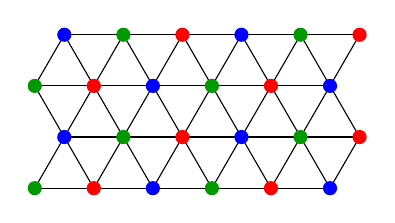
\begin{tikzpicture}[scale=0.75]
  \foreach \j in {0,1,2,3} \draw ({0.5*mod(\j,2)},{0.866*\j}) -- ++(5,0);
  \foreach \i in {0,...,5} {\draw (\i,0) -- ++(60:1) -- ++(120:1) -- ++(60:1);}
  \foreach \i in {1,...,5} {\draw (\i,0) -- ++(120:1) -- ++(60:1) -- ++(120:1);}
  \foreach \j in {0,1,2,3} \foreach \i in {0,...,5} {
    \pgfmathtruncatemacro{\c}{mod(\i-floor(\j/2)-\j+30,3)}
    \pgfmathsetmacro{\xx}{\i+0.5*mod(\j,2)}
    \ifnum\c=0 \fill[green!60!black] (\xx,{0.866*\j}) circle (0.12);\fi
    \ifnum\c=1 \fill[red] (\xx,{0.866*\j}) circle (0.12);\fi
    \ifnum\c=2 \fill[blue] (\xx,{0.866*\j}) circle (0.12);\fi
  }
\end{tikzpicture}
\diagramcaption{One ground state of krypton on graphite, drawn on the dual triangular lattice. Green sites are Kr atoms;
each is surrounded by vacant faces of $\Lambda_{hc}$, i.e.\ vacant sites of $\Lambda_{hc}^* = \Lambda_{tri}$. The three
colors mark the three sublattices of $\Lambda_{tri}$.}
\end{diagram}

The picture shows one ground state of the system, with each Kr atom (indicated by green) surrounded by vacant faces of
$\Lambda_{hc}\leftrightarrow$ vacant sites of $\Lambda_{hc}^* = \Lambda_{tri}$. This is called ``$\frac13$ coverage'', since
$\frac13$ of the faces of $\Lambda_{hc}$ (i.e.\ $\frac13$ of the sites of $\Lambda_{tri}$) are occupied by the Kr atoms. Since
$\Lambda_{tri} = \Lambda_1\oplus\Lambda_2\oplus\Lambda_3$ (green, red and blue sublattices), there are two other equivalent
ground states, where the Kr atoms are adsorbed on the other set of faces of $\Lambda_{hc}$ (graphene surface), i.e.\ the
vertices on the other two sublattices of $\Lambda_{tri}$ (red or blue). This is equivalent to the 3 degenerate ground states
of the $q = 3$ ferromagnetic Potts model with $\sigma_i = 1$, 2, or 3 $\forall\,i$. So this system can be described by this
model.

% Source: Lecture8.pdf, pages 1-21 (typed handout). Title on the source: "Lecture 8: Further
% Properties of Potts Model Partition Functions and Connections with Graph-Theoretic Polynomials".
\lecture{8}
\subsection{Some preliminaries from graph theory}

A graph $G$ is defined by its set of vertices (sites, in physics terminology), $V = \{v_1,\ldots,v_{n(G)}\}$ and its set of
edges (bonds in physics terminology), $E$, so we write $G = (V,E)$. The total numbers of vertices and edges in $G$ are
$n(G)$ and $e(G)$, respectively.

\paragraph{Def.} A graph $G$ is \emph{connected} if, starting at a given vertex $v\in V$, there exists a continuous path along
the edges that enables one to move to any other vertex in $V$. For a general graph, we denote $k(G)$ as the number of
connected components of $G$. An example of a connected graph is the line graph $L_3$ consisting of three vertices $v_i$,
$i = 1,2,3$ with an edge $e_{12}$ connecting $v_1$ and $v_2$, and an edge $e_{23}$ connecting $v_2$ and $v_3$. An example
of a disconnected graph is obtained by deleting either of these two edges; the resultant graph has $k = 2$ components. If
one deletes both edges, the resultant graph has $k = 3$ components.

\paragraph{Def.} The \emph{empty} (null) graph $E_n$ is the graph consisting of $n$ vertices with no edges.

\paragraph{Def.} The \emph{complete graph} $K_n$ is the graph consisting of $n$ vertices such that there is a (single) edge
$e_{ij}$ connecting each distinct pair of vertices $v_i$ and $v_j$.

\paragraph{Def.} A \emph{bridge} on a graph is an edge such that deleting it leads to an increase in the number of components
in the graph. For example, consider the line graph $L_3$ with three vertices. This is a connected graph, so $k(L_3) = 1$.
Both of its two edges are bridges, since deleting either one produces a graph with $k = 2$ connected components.

\paragraph{Def.} A \emph{loop} is an edge that extends out from a given vertex and loops back to connect to the same vertex.
In physics we will usually restrict to loopless graphs.

\paragraph{Def.} Two vertices in $G$ are said to be \emph{adjacent} if they are connected by at least one edge. In general,
two adjacent vertices may be connected by more than one edge, although on a regular lattice one generally restricts to the
minimal case in which adjacent vertices are connected by only one edge.

\paragraph{Def.} The \emph{degree} $\Delta_v$ of a vertex $v$ in $G$ is equal to the number of edges that connect to it.

\paragraph{Def.} A graph $G$ is said to be \emph{$\Delta$-regular} if all of its vertices have the same degree, $\Delta$. A 1D
lattice with periodic boundary conditions (BC) is a 2-regular graph. A 2D square lattice with toroidal boundary conditions
is a 4-regular graph, etc. On a $\Delta$-regular lattice graph $\Lambda$, $\Delta_\Lambda$ is the coordination number of the
lattice. For a $\Delta$-regular lattice graph,
\begin{equation}
  e(G) = \frac\Delta2n(G).
\end{equation}
One can also define an effective degree $\Delta_{\text{eff}}$ of a graph as
\begin{equation}
  \Delta_{\text{eff}} = \lim_{n(G)\to\infty}\frac{2e(G)}{n(G)}.
\end{equation}
For example, consider a 1D lattice with free boundary conditions; then the interior vertices have degree $\Delta = 2$, but
the end vertices have degree $\Delta = 1$, so this is not a $\Delta$-regular graph. However, in the limit as
$n(G)\to\infty$, $\Delta_{\text{eff}} = 2$. Similarly, consider a rectangular $L_x\times L_y$ section of a 2D square lattice
with free boundary conditions. Then the interior vertices have degree 4, the other vertices on the four sides have degree 3,
and the corner vertices have degree 2. Again, in the thermodynamic limit $L_x\to\infty$ and $L_y\to\infty$ with finite
nonzero aspect ratio $L_y/L_x$, $\Delta_{\text{eff}} = 4$. This is thus the same as if one used boundary conditions that are
periodic in one direction (sometimes called cylindrical) or in both directions (toroidal BC). Similar comments apply for
higher-dimensional lattices.

\paragraph{Def.} The graph $C_n$ with $n$ vertices is called the \emph{circuit graph}. It is equivalent to a 1D lattice with
$n$ vertices and PBC.

\paragraph{Def.} A \emph{cycle} (circuit) in $G$ is a path on adjacent edges that forms a circuit. The number of linearly
independent cycles on $G$ is denoted $c(G)$. For example, consider the circuit graph $C_4$ with vertex set
$\{v_1,v_2,v_3,v_4\}$. We can think of this as a square with the lower right-hand vertex denoted $v_1$, the upper right-hand
vertex denoted $v_2$, etc. Now add one diagonal edge (bond) joining the upper right-hand vertex $v_2$ to the lower left-hand
vertex $v_4$. The resultant graph $G$ has $n(G) = 4$, edge set $E = \{e_{12},e_{23},e_{34},e_{41},e_{24}\}$ and
$e(G) = 5$. There are three cyclic paths that one can draw: (i) around the outside of the square; (ii) around the upper
left-hand triangle; and (iii) around the lower right-hand triangle. However, only two of these are linearly independent, so
$c(G) = 2$. (Recall similar considerations when using Kirchhoff's laws in electrical circuits; if this were a circuit with
resistors, one would only write down two linearly independent Kirchhoff equations.) A relevant relation is
\begin{equation}
  c(G) = e(G) + k(G) - n(G);
\end{equation}
for example, for the graph above, $n(G) = 4$, $e(G) = 5$, and $k(G) = 1$, so $c(G) = 5+1-4 = 2$.

\paragraph{Def.} A \emph{tree graph} is a connected graph with no cycles. Although the tree graphs with $n = 1,2,3$ are unique,
for $n\ge 4$, there is more than one tree graph. For example, for $n = 4$, there are two tree graphs, namely the line graph
with 4 vertices and the star graph with one central vertex and three outer vertices. We sometimes use the generic symbol $T_n$
for an $n$-vertex tree graph.

\paragraph{Def.} Given a graph $G = (V,E)$, a \emph{spanning subgraph} $G' = (V',E')$ is a graph containing all of the vertices
of $G$, so $V' = V$, and a subset of the edges of $G$, i.e.\ $E'\subseteq E$.

\paragraph{Def.} A graph is \emph{planar} if it can be embedded in a plane with no intersecting edges.

\paragraph{Def.} Given a planar graph $G$, the \emph{planar dual} of $G$, denoted $G^*$, is obtained by mapping each face in $G$
to a vertex in $G^*$, each vertex in $G$ to a face in $G^*$, and then connecting the vertices of $G^*$ with edges. A planar
graph $G$ is self-dual if $G^* = G$.

\subsection{Cluster formula for the Potts model partition function}

Let us consider the Potts model on a general graph $G = (V,E)$. Formulated in the context of statistical mechanics, this
model involves dynamical variables (classical spins) $\sigma_i$ at each vertex $v_i\in V$ that can take on any of the values
in the set $\{1,\ldots,q\}$, with an interaction energy between the spins on adjacent vertices
$\Ham_{\text{int}} = -J\sum_{e_{ij}}\delta_{\sigma_i\sigma_j}$. For simplicity, let us take the external magnetic field to be
zero. Then $\Ham = \Ham_{\text{int}}$ and $-\beta\Ham = K\sum_{e_{ij}}\delta_{\sigma_i\sigma_j}$, where $K = \beta J$ and
$\beta = 1/(\kB T)$, with $T$ the temperature. In thermal equilibrium at a temperature $T$, the partition function is
\begin{equation}
  Z = \sum_{\{\sigma_i\}}e^{-\beta\Ham} = \sum_{\{\sigma_i\}}\exp\left[K\sum_{e_{ij}}\delta_{\sigma_i\sigma_j}\right].
\end{equation}
Let $v_P = e^K-1$ and, for notational simplicity, suppress the subscript $P$, writing this as $v$. Recall the identity
\begin{equation}
  e^{K\delta_{\sigma_i\sigma_j}} = 1 + \left(e^K-1\right)\delta_{\sigma_i\sigma_j} = 1 + v\delta_{\sigma_i\sigma_j}.
\end{equation}
Using this identity, we can write $Z$ as
\begin{equation}
  Z = \sum_{\{\sigma_i\}}\left[\prod_{e_{ij}}\left(1+v\delta_{\sigma_i\sigma_j}\right)\right].
\end{equation}
As above, let $G'$ denote a spanning subgraph of $G$. Then one can rewrite $Z$ as
\begin{equation}\label{eq:cluster}
  Z(G,q,v) = \sum_{G'\subseteq G}q^{k(G')}v^{e(G')},
\end{equation}
where $k(G')$ and $e(G')$ are the number of connected components and edges in $G'$. This is often called the
Fortuin--Kasteleyn cluster formula for the Potts model partition function by physicists, although an equivalent relation had
been derived earlier by mathematicians. This cluster formula is very useful, since it expresses $Z$ in a graph-theoretic
manner, as a sum over contributions from spanning subgraphs without explicit reference to the sum over spin configurations.

If $G$ is the disjoint union $G = G_1\cup G_2$, then $Z(G,q,v) = Z(G_1,q,v)Z(G_2,q,v)$ so, without loss of generality, we
take $G$ to be connected. (But some $G'$ subgraphs are disconnected.)

Since $k(G')\ge 1$ and $e(G')\ge 0$, the cluster representation of $Z$ shows that $Z(G,q,v)$ is a polynomial in $q$ and $v$.

\paragraph{Corollary.} Since $k(G')\ge 1$, the minimum degree of $Z$ as a polynomial in $q$ is 1, i.e.\ $Z(G,q,v)$ always
contains an overall factor of $q$. Since one of the spanning subgraphs is the empty graph with no edges, the minimum degree of
$Z$ as a polynomial in $v$ is 0.

The cluster formula allows one to formally generalize $q$ from nonnegative integers $q = 1,2,3,\ldots$ to nonnegative real
numbers. For the case of ferromagnetic spin--spin couplings, $v\ge 0$, the resultant $Z$ is nonnegative, and is positive if
$q\ne 0$. Physically, since $\Ham$ is real, the Boltzmann weights $e^{-\beta\Ham}$ are nonnegative. One refers to this situation
by saying that a model has a ``Gibbs measure''. So (aside from the marginal case $q = 0$), the generalization above in the case
of the FM sign of the coupling, $J>0$, yields a Gibbs measure.

If one is interested in zeros of $Z$ in the variable $q$, then one naturally generalizes $q$ to complex numbers, but for most of
our discussion, the generalization to real nonnegative $q$ will be sufficient.

\subsubsection*{Proof of the cluster formula}

The proof of the cluster formula is based on the 1--1 correspondence between the terms in
$Z = \sum_{\{\sigma_i\}}\prod_{e_{ij}}\left(1+v\delta_{\sigma_i\sigma_j}\right)$ and spanning subgraphs $G'\subseteq G$. A sketch of
the proof, using, as illustration, $G = C_3$, where $C_n$ is the circuit graph with $n$ vertices. Here
\begin{equation}
  Z(C_3,q,v) = \sum_{\{\sigma_i\}}\prod_{e_{ij}}\left(1+v\delta_{\sigma_i\sigma_j}\right)
  = \sum_{\{\sigma_i\}}\left(1+v\delta_{\sigma_1\sigma_2}\right)\left(1+v\delta_{\sigma_2\sigma_3}\right)\left(1+v\delta_{\sigma_3\sigma_1}\right).
\end{equation}
There are four types of terms that contribute (in correspondence with $\sum_{G'\subseteq G}q^{k(G')}v^{e(G')}$):
\begin{itemize}
  \item the term 1, corresponding to the $G'$ with three disjoint vertices, no edges (so $e(G') = 0$, $k(G') = 3$), for which
    the sum over the $\sigma_i$'s yields $q^3$, i.e.\ one can choose the $\sigma$'s independently in $q^3$ ways;
  \item $v\left(\delta_{\sigma_1\sigma_2}+\delta_{\sigma_2\sigma_3}+\delta_{\sigma_3\sigma_1}\right)$, corresponding to the three
    $G'$s with one edge and one disjoint vertex, so $e(G') = 1$, $k(G') = 2$. The first of these terms contributes if
    $\sigma_1 = \sigma_2$; here one chooses $\sigma_1 = \sigma_2$ in any of $q$ ways, and then $\sigma_3$ independently in any
    of $q$ ways, for a total of $q^2$ ways; similarly for the other two terms, so these terms contribute $3q^2v$;
  \item $v^2\left(\delta_{\sigma_1\sigma_2}\delta_{\sigma_2\sigma_3}+\delta_{\sigma_2\sigma_3}\delta_{\sigma_3\sigma_1}
    +\delta_{\sigma_3\sigma_1}\delta_{\sigma_1\sigma_2}\right)$, corresponding to $G'$s with two edges, so $e(G') = 2$,
    $k(G') = 1$. For the first term to contribute, all of the $\sigma$'s must be equal, and there are $q$ ways of choosing
    them; similarly for the other two terms, so the total contribution is then $3qv^2$;
  \item $v^3\left(\delta_{\sigma_1\sigma_2}\delta_{\sigma_2\sigma_3}\delta_{\sigma_3\sigma_1}\right)$, corresponding to $G' = G$,
    with all edges present, so $e(G') = 3$, $k(G') = 1$. For this term to contribute, all of the $\sigma$'s must be equal,
    amounting to $q$ possibilities, and yielding the term $qv^3$.
\end{itemize}
So combining all of these terms, one gets $Z(C_3,q,v) = q^3+3q^2v+3qv^2+qv^3$, which is precisely
$\sum_{G'\subseteq C_3}q^{k(G')}v^{e(G')}$. Now
\begin{equation}
  q^3+3q^2v+3qv^2+qv^3 = q^3+3q^2v+3qv^2+v^3+qv^3-v^3 = (q+v)^3+(q-1)v^3,
\end{equation}
so $Z(C_3,q,v) = (q+v)^3+(q-1)v^3$. By the same methods, one obtains the generalization
\begin{equation}
  Z(C_n,q,v) = (q+v)^n+(q-1)v^n .
\end{equation}
We derived this inductively in the last lecture using transfer-matrix methods, where we showed that the $q\times q$ transfer
matrix on a 1D lattice with PBC has one (leading) eigenvalue $\lambda_1 = q+v$ and a subleading eigenvalue $\lambda_2 = v$ with
multiplicity $q-1$, so $Z(C_n,q,v) = \lambda_1^n+(q-1)\lambda_2^n = (q+v)^n+(q-1)v^n$. In that derivation, $q$ had to be a
positive integer. Our present derivation does not require $q$ to be a positive integer and hence is more general.

\subsection{Chromatic and Tutte polynomials}

Next, let us define two important graph-theoretic polynomials.

\paragraph{Def.} The \emph{chromatic polynomial} $P(G,q)$ is the number of ways of assigning $q$ colors to the vertices of $G$
such that no two adjacent vertices have the same color. This is called a proper $q$-coloring of (the vertices of) $G$. The
minimum number of colors needed for a proper $q$-coloring of $G$ is the chromatic number, $\chi(G)$.

Note that if a graph contains any loop, then $P(G,q)$ vanishes identically, since a vertex with a loop is adjacent to itself,
so it cannot satisfy the constraint that it has a different color than adjacent vertices.

In the antiferromagnetic Potts model, consider the limit $T\to 0$, so $K\to-\infty$ (since $K = \beta J$ and $J<0$) and
$v = e^K-1\to-1$. In this limit, the only spin configurations that contribute to $Z(G,q,v=-1)$ are those for which adjacent
spins have different values. Hence, the $T = 0$ limit of the Potts antiferromagnet partition function is the chromatic
polynomial:
\begin{equation}
  Z(G,q,-1) = P(G,q).
\end{equation}
Since $Z(G,q,v)$ always contains an overall factor of $q$, this is also true for $P(G,q)$. Given the meaning of $P(G,q)$ as the
number of proper $q$-colorings of $G$, the fact that $P(G,0) = 0$ is clear.

There is a close connection between the Potts model partition function and a function of major importance in mathematical
graph theory, the Tutte (also called Tutte--Whitney) polynomial, $T(G,x,y)$.

\paragraph{Def.} The \emph{Tutte polynomial} of a graph $G$ is
\begin{equation}
  T(G,x,y) = \sum_{G'\subseteq G}(x-1)^{k(G')-k(G)}(y-1)^{c(G')}
           = \sum_{G'\subseteq G}(x-1)^{k(G')-k(G)}(y-1)^{e(G')+k(G')-n(G')},
\end{equation}
where $G'$ is a spanning subgraph of $G$ and $k(G')$ and $c(G')$ denote the number of components and (linearly independent)
cycles in $G'$. Since $k(G')-k(G)\ge 0$ and $c(G')\ge 0$, it follows that $T(G,x,y)$ is a polynomial in $x$ and $y$.

To prove this connection (essentially an equivalence with appropriate changes of variables), let
\begin{equation}
  x = 1+\frac qv,\qquad y = v+1,
\end{equation}
so $q = (x-1)(y-1)$ and $v = y-1$. Then, using the fact that $n(G') = n(G)$, so
$c(G') = e(G')+k(G')-n(G') = e(G')+k(G')-n(G)$, and $x-1 = q/v$, $y-1 = v$, we have
\begin{align}
  T(G,x,y) &= (x-1)^{-k(G)}(y-1)^{-n(G)}\sum_{G'\subseteq G}(x-1)^{k(G')}(y-1)^{e(G')+k(G')}\nonumber\\
  &= (x-1)^{-k(G)}(y-1)^{-n(G)}\sum_{G'\subseteq G}\left(\frac qv\right)^{k(G')}v^{e(G')+k(G')}\nonumber\\
  &= (x-1)^{-k(G)}(y-1)^{-n(G)}\sum_{G'\subseteq G}q^{k(G')}v^{e(G')}\nonumber\\
  &= (x-1)^{-k(G)}(y-1)^{-n(G)}Z(G,q,v),
\end{align}
i.e.
\begin{equation}
  Z(G,q,v) = (x-1)^{k(G)}(y-1)^{n(G)}T(G,x,y) = \left(\frac qv\right)^{k(G)}v^{n(G)}T(G,x,y).
\end{equation}

\subsubsection*{Special valuations of the Tutte polynomial}

Special valuations of $T(G,x,y)$ count various types of subgraphs of $G$. Setting $x = 1$ in $T(G,x,y)$ restricts the $G'$s
that contribute to those that are connected, i.e.\ $k(G') = k(G) = 1$. Setting $y = 1$ restricts the $G'$s that contribute to
those having no cycles, so that $c(G') = 0$.

\paragraph{Def.} A connected spanning subgraph that is a tree (is cycle-free, $c(G') = 0$) is called a \emph{spanning tree}.
Setting $x = y = 1$ picks out $G'$s that are connected spanning subgraphs with $c(G') = 0$, i.e.\ spanning trees. So
\begin{equation}
  T(G,1,1) = N_{ST}(G).
\end{equation}

\paragraph{Def.} A spanning subgraph $G'$ that has no cycles but may be disconnected, i.e.\ consist of more than one component,
is called a \emph{spanning forest} of $G$. One can relax the restriction on connectedness by setting $x = 2$, so that
$(x-1)^{k(G')-k(G)} = 1$, independent of $k(G')$. Then
\begin{equation}
  T(G,2,1) = N_{SF}(G),
\end{equation}
where $N_{SF}(G)$ is the number of spanning forests of $G$.

One can keep the restriction on connectedness but include $G'$s with cycles by setting $y = 2$; then $(y-1)^{c(G')} = 1$
independent of $c(G')$. Hence
\begin{equation}
  T(G,1,2) = N_{CSSG}(G),
\end{equation}
where $N_{CSSG}$ is the number of connected spanning subgraphs of $G$. If one sets $x = y = 2$, then the summand is just 1, so
this counts all of the spanning subgraphs of $G$: $T(G,2,2) = 2^{e(G)}$.

Special cases of the Tutte polynomial yield many graph-theoretic functions of interest. One of these is the chromatic
polynomial; for $v = -1$, i.e.\ $y = 0$, since $Z(G,q,v=-1) = P(G,q)$, one has
\begin{equation}
  P(G,q) = (-q)^{k(G)}(-1)^{n(G)}\,T(G,x=1-q,y=0).
\end{equation}

\subsection{Coloring problems and the four-color theorem}

The chromatic polynomial is of interest not just in graph theory but also in applied mathematics and engineering. One
application is the following frequency allocation problem. Consider $n$ radio broadcast transmitter stations; let each of these
be represented by a vertex of a graph $G$ and define two transmitters as being adjacent (joined by an edge) if they are closer
than a certain distance to each other. Then assign frequencies from a set of $q$ values to these transmitters, subject to the
condition that adjacent stations should use different frequencies to avoid interference. The number of ways of doing this is
$P(G,q)$.

The early interest by Birkhoff and Whitney in chromatic polynomials was motivated by their connection with the map coloring
problem, i.e.\ face-colorings of graphs; further work was done by Tutte, Read, and others.

\paragraph{Def.} A \emph{proper $q$-coloring of the faces} of a graph is an assignment of colors, from a set of $q$ colors, to the
faces of a graph such that no two adjacent faces (faces that share an edge) have the same color.

As we noted, for a planar graph $G$, there is a 1--1 correspondence between the vertices of $G$ and the faces of the planar dual
graph $G^*$. Therefore, $P(G,q)$ equivalently counts the proper $q$-colorings of the vertices of $G$ and the proper
$q$-colorings of the faces of $G^*$.

Recall that an edge of a graph such that its deletion would increase the number of components by 1 is called a bridge. A
bridge in a planar graph leads to a face being adjacent to itself across the bridge. Since adjacent faces must have different
colors in a proper $q$-coloring of the faces of a planar graph $G^*$, this is not possible if $G^*$ contains any bridges. This is
the planar dual of the property that a proper $q$-coloring of a graph $G$ is not possible if the graph contains any loops.

The \emph{Four-Color Theorem} is the statement that if $G$ is a planar graph with no loops, so $G^*$ is a planar graph with no
bridges, then $P(G,4)>0$, i.e.\ there exists a proper $q$-coloring of the faces of $G^*$ with $q = 4$ colors; equivalently,
there exists a proper $q$-coloring of the vertices of $G$ with $q = 4$ colors. Mathematicians sought to prove this for over a
century. It was proved in 1976 by Appel and Haken.

\subsection{Simple examples of \texorpdfstring{$Z(G,q,v)$, $T(G,x,y)$ and $P(G,q)$}{Z, T and P}}

We have shown that for a circuit graph, $C_n$, $Z(C_n,q,v) = (q+v)^n+(q-1)v^n$. Using $x-1 = q/v$ and $q = (x-1)(y-1)$, we
can write this as
\begin{equation}
  Z(C_n,q,v) = v^n\left[\left(1+\frac qv\right)^n+(q-1)\right] = v^n\left[x^n+(q-1)\right]
  = \left(\frac qv\right)v^n\left[\frac{x^n+(q-1)}{x-1}\right],
\end{equation}
and hence we have
\begin{equation}
  T(C_n,x,y) = \left[\frac{x^n+(xy-y-x)}{x-1}\right].
\end{equation}
Using $(x^n-x)/(x-1) = \sum_{j=1}^{n-1}x^j$ (for $n\ge 2$), one can write this as
\begin{equation}
  T(C_n,x,y) = \left(\sum_{j=1}^{n-1}x^j\right)+y .
\end{equation}
As is the case here, in expressions for $T(G,x,y)$ with a $1/(x-1)$ prefactor, it is always cancelled, so that $T(G,x,y)$ is a
polynomial in $x$ and $y$.

Setting $v = -1$ in the results for $Z(G,q,v)$ yields $P(G,q)$. For example, from $Z(C_n,q,v) = (q+v)^n+(q-1)v^n$, it follows
that
\begin{equation}
  P(C_n,q) = (q-1)^n+(q-1)(-1)^n .
\end{equation}

Many properties of $P(G,q)$ can be proved by combinatoric arguments. For example, if a graph $G$ contains any edge (i.e.\ is
not the null graph, $E_n$), then $P(G,q)$ clearly vanishes if $q = 1$, since one would have to use at least two colors to
assign different colors to the vertices that are adjacent along this edge. This, together with the property that $P(G,q)$ is a
polynomial in $q$, proves that, in addition to the factor of $q$ that it always contains, $P(G,q)$ also contains a factor of
$q-1$.

Similarly, if a graph $G$ contains any subgraph that is isomorphic to a triangle, $K_3 = C_3$, then $P(G,q)$ contains not just
the factors of $q$ and $q-1$, but also a factor of $q-2$. This is proved by noting that one can choose the color assigned to
the first vertex of the $K_3$ subgraph in any of $q$ ways, but then one can choose the color of the second vertex in $K_3$ in
only $q-1$ ways, and one can choose the color of the third vertex in the $K_3$ subgraph in only $q-2$ ways. So if $q = 2$, then
$P(G,q) = 0$. Since $P(G,q)$ is a polynomial, this proves that it contains a factor of $q-2$.

\paragraph{Def.} A graph is \emph{$k$-partite} if the vertex set $V$ can be partitioned as $V = V_1\cup V_2\cup\cdots\cup V_k$,
where $V_i\cap V_j = \emptyset$ if $i\ne j$ and no vertex in $V_i$ connects via an edge to any other vertex in $V_i$ for any $i$.

Another simple result is the following: for a connected bipartite graph $G_{\text{bip.}}$,
\begin{equation}
  P(G_{\text{bip.}},q=2) = 2 .
\end{equation}
This is proved by noting that one can choose the color to be assigned to a vertex in $V_1$ in any of 2 ways. Then one must
assign the other color to all of the vertices in $V_2$, and the first color to all the other vertices of $V_1$. As we have
discussed, the circuit graph $C_n$ is bipartite if and only if $n$ is even. By similar combinatoric arguments, one has
$P(G_{tri},3) = 3!$, where $tri$ is the triangular lattice, with free boundary conditions. To prove this, one assigns the three
colors to the vertices of one triangle, for which there are $3!$ ways. This uniquely determines the color assignments to all
other triangles on the lattice.

% Source: Lecture8a.pdf, pages 1-4 (page 1 is a title page; page 5 is blank). Title on the source:
% "Lecture 8a (to be used in conjunction with the printed slides in Lecture 8)".
\lecture{8a}
\subsection{Further notes for Lecture 8: examples of graphs}

These notes are to be used in conjunction with the printed slides of Lecture 8.

\tikzset{gv/.style={circle,fill,inner sep=0pt,minimum size=4pt}}

\begin{diagram}
\begin{tikzpicture}[scale=0.8]
  \node[anchor=east] at (-0.3,0) {empty graph $E_3$:};
  \foreach \x/\l in {0/v_3,0.6/v_2,1.2/v_1} {\node[gv] at (\x,0) {}; \node[below,font=\scriptsize] at (\x,-0.05) {$\l$};}
  \node[blue,anchor=west,font=\small] at (1.6,0) {$k(E_3) = 3$};
  \begin{scope}[yshift=-1.3cm]
    \node[anchor=east] at (-0.3,0) {line graph $L_3$:};
    \draw (0,0) -- (1.2,0);
    \foreach \x/\l in {0/v_3,0.6/v_2,1.2/v_1} {\node[gv] at (\x,0) {}; \node[below,font=\scriptsize] at (\x,-0.05) {$\l$};}
    \node[above,font=\scriptsize] at (0.3,0) {$e_{23}$}; \node[above,font=\scriptsize] at (0.9,0) {$e_{21}$};
    \node[blue,anchor=west,font=\small] at (1.5,0) {(both edges are bridges)};
  \end{scope}
  \begin{scope}[yshift=-2.7cm]
    \node[anchor=east] at (-0.3,0) {$L_4$:};
    \draw (0,0) -- (1.8,0); \foreach \x in {0,0.6,1.2,1.8} \node[gv] at (\x,0) {};
    \begin{scope}[xshift=1.2cm]
    \node[anchor=east] at (4.5,0.1) {star graph $S_4$:};
    \draw (5.7,0) -- (5.7,0.7); \draw (5.7,0) -- (5.1,-0.35); \draw (5.7,0) -- (6.3,-0.35);
    \foreach \p in {(5.7,0),(5.7,0.7),(5.1,-0.35),(6.3,-0.35)} \node[gv] at \p {};
    \node at (6.8,0) {$=$};
    \draw (7.2,0) -- (8.4,0); \draw (7.8,0) -- (7.8,0.6);
    \foreach \p in {(7.2,0),(7.8,0),(8.4,0),(7.8,0.6)} \node[gv] at \p {};
    \draw[decorate,decoration={brace,amplitude=5pt}] (8.8,0.8) -- (8.8,-0.5);
    \node[anchor=west,font=\small,align=left] at (9.0,0.15) {the two tree\\ graphs with $n = 4$\\ vertices, $T_4$};
    \end{scope}
  \end{scope}
\end{tikzpicture}
\diagramcaption{Some types of graphs.}
\end{diagram}

\begin{diagram}
\begin{tikzpicture}[scale=0.8]
  % circuit graphs
  \node[gv] (a) at (0,0) {}; \draw (0,0) .. controls (-0.5,0.9) and (0.5,0.9) .. (0,0);
  \node[below] at (0,-0.4) {$C_1$}; \node[blue,font=\scriptsize] at (-0.6,0.8) {loop};
  \draw (1.6,0.25) circle (0.45); \node[gv] at (1.15,0.25) {}; \node[gv] at (2.05,0.25) {}; \node[below] at (1.6,-0.4) {$C_2$};
  \draw (3.4,0.25) circle (0.45); \foreach \a in {90,210,330} \node[gv] at ($(3.4,0.25)+(\a:0.45)$) {}; \node[below] at (3.4,-0.4) {$C_3$};
  \draw (5.2,0.25) circle (0.45); \foreach \a in {45,135,225,315} \node[gv] at ($(5.2,0.25)+(\a:0.45)$) {};
  \node at (6.0,0.25) {$=$}; \draw (6.4,-0.1) rectangle (7.1,0.6);
  \foreach \p in {(6.4,-0.1),(7.1,-0.1),(6.4,0.6),(7.1,0.6)} \node[gv] at \p {};
  \node[below] at (5.8,-0.4) {$C_4$};
  \node at (3.5,1.3) {circuit graphs};
  % complete graphs
  \begin{scope}[xshift=8.6cm]
    \node at (2.4,1.3) {complete graphs};
    \draw (0,0.25) -- (0.8,0.25); \node[gv] at (0,0.25) {}; \node[gv] at (0.8,0.25) {};
    \node[below] at (0.4,-0.4) {$K_2 = L_2$};
    \draw (2.0,-0.1) -- (2.8,-0.1) -- (2.4,0.6) -- cycle;
    \foreach \p in {(2.0,-0.1),(2.8,-0.1),(2.4,0.6)} \node[gv] at \p {};
    \node[below] at (2.4,-0.4) {$K_3 = C_3$};
    \coordinate (A) at (3.8,-0.1); \coordinate (B) at (4.8,-0.1); \coordinate (Cc) at (4.3,0.75); \coordinate (D) at (4.3,0.2);
    \draw (A) -- (B) -- (Cc) -- cycle; \draw (A) -- (D) -- (B); \draw (Cc) -- (D);
    \foreach \p in {A,B,Cc,D} \node[gv] at (\p) {};
    \node[below] at (4.3,-0.4) {$K_4$};
  \end{scope}
\end{tikzpicture}
\diagramcaption{Circuit graphs $C_n$ and complete graphs $K_n$.}
\end{diagram}

\paragraph{Cycles in a graph.} For the square with one diagonal,
\begin{equation}
  c(G) = e(G)+k(G)-n(G) = 5+1-4 = 2 .
\end{equation}
There are 3 cycles, but only 2 are linearly independent; by combining the inner two cycles, one obtains the outer cycle.

\begin{diagram}
\begin{tikzpicture}[scale=0.9]
  \draw (0,0) rectangle (1.4,1.4); \draw (0,0) -- (1.4,1.4);
  \foreach \p in {(0,0),(1.4,0),(0,1.4),(1.4,1.4)} \node[gv] at \p {};
  \draw[blue,->] (0.15,0.95) arc (180:-120:0.2);
  \draw[blue,->] (0.85,0.25) arc (180:-120:0.2);
  \draw[blue,->,rounded corners] (-0.2,-0.2) rectangle (1.6,1.6);
\end{tikzpicture}
\diagramcaption{The square with a diagonal edge: two independent inner cycles and the outer cycle.}
\end{diagram}

\subsection{Spanning subgraphs and the Tutte polynomial of \texorpdfstring{$C_3$}{C3}}

Spanning subgraphs (SSG): e.g.\ let $G = C_3 = K_3$; $G = (V,E)$; $G' = (V,E')$, $E'\subseteq E$. The spanning subgraphs
$\{G'\}$ are:

\begin{diagram}
\begin{tikzpicture}[scale=0.8]
  \newcommand{\tri}[4]{%
    \begin{scope}[xshift=#1 cm]
      \coordinate (P1) at (0,0); \coordinate (P2) at (0.9,0); \coordinate (P3) at (0.45,0.78);
      \foreach \p in {P1,P2,P3} \node[gv] at (\p) {};
      \ifnum#2=1 \draw (P1) -- (P2);\fi
      \ifnum#3=1 \draw (P2) -- (P3);\fi
      \ifnum#4=1 \draw (P3) -- (P1);\fi
    \end{scope}}
  \tri{0}{1}{1}{1}
  \node[font=\small,align=center] at (0.45,-0.7) {$k = 1$\\ $e = 3$};
  \tri{2.0}{1}{1}{0} \tri{3.3}{0}{1}{1} \tri{4.6}{1}{0}{1}
  \node[font=\small] at (3.75,-0.5) {$k = 1$, $e = 2$};
  \tri{6.6}{1}{0}{0} \tri{7.9}{0}{1}{0} \tri{9.2}{0}{0}{1}
  \node[font=\small] at (8.35,-0.5) {$k = 2$, $e = 1$};
  \tri{11.2}{0}{0}{0}
  \node[font=\small,align=center] at (11.65,-0.65) {$k = 3$, $e = 0$};
  \node[font=\small,anchor=south] at (11.65,1.0) {$E_3$};
  \node[blue,font=\scriptsize] at (0.45,1.2) {CSSG};
  \node[blue,font=\scriptsize] at (3.75,1.2) {spanning trees, ST};
  \draw[blue,decorate,decoration={brace,amplitude=4pt,mirror}] (2.0,-1.25) -- (12.1,-1.25);
  \node[blue,font=\scriptsize] at (7.0,-1.6) {spanning forests, SF};
\end{tikzpicture}
\diagramcaption{The $2^3 = 8$ spanning subgraphs of $C_3$. CSSG = connected spanning subgraphs. Note: one of the $G'$ is $G$
itself.}
\end{diagram}

From $T(C_n,x,y) = \left[\sum_{j=1}^{n-1}x^j\right]+y$,
\begin{equation}
  T(C_3,x,y) = x+x^2+y,
\end{equation}
and
\begin{align}
  T(C_3,1,1) &= N_{ST}(C_3) = 3, & T(C_3,1,2) &= N_{CSSG}(C_3) = 4,\\
  T(C_3,2,1) &= N_{SF}(C_3) = 7, & T(C_3,2,2) &= N_{SSG}(C_3) = 8 .
\end{align}

\subsection{\texorpdfstring{$k$}{k}-partite graphs}

$k$-partite graphs: $G = G(V,E)$ such that $V = V_1\cup V_2\cup\cdots\cup V_k$, where $\{V_i\}$ are subsets of $V$, such that no
edge connects a vertex in $V_i$ to another vertex in $V_i$. Any loopless $n$-vertex graph is $n$-partite with $V_i = \{v_i\}$.
Examples of bipartite graphs: the line graph $L_n$ for any $n$; the circuit graph $C_n$ if $n$ is even, but not $C_n$, $n$ odd.
Tripartite examples: $L_3$ (colored with three colors) and the triangular lattice with free boundary conditions (FBC).

\begin{diagram}
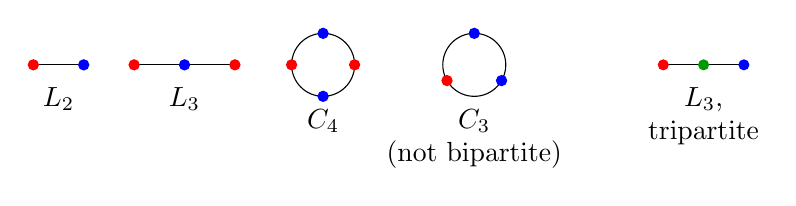
\begin{tikzpicture}[scale=0.8]
  \draw (0,0) -- (0.8,0); \fill[red] (0,0) circle (0.09); \fill[blue] (0.8,0) circle (0.09); \node[below] at (0.4,-0.2) {$L_2$};
  \draw (1.6,0) -- (3.2,0); \fill[red] (1.6,0) circle (0.09); \fill[blue] (2.4,0) circle (0.09); \fill[red] (3.2,0) circle (0.09);
  \node[below] at (2.4,-0.2) {$L_3$};
  \draw (4.6,0) circle (0.5);
  \fill[blue] (4.6,0.5) circle (0.09); \fill[red] (5.1,0) circle (0.09); \fill[blue] (4.6,-0.5) circle (0.09); \fill[red] (4.1,0) circle (0.09);
  \node[below] at (4.6,-0.55) {$C_4$};
  \draw (7.0,0) circle (0.5);
  \fill[blue] (7.0,0.5) circle (0.09); \fill[red] ($(7.0,0)+(210:0.5)$) circle (0.09); \fill[blue] ($(7.0,0)+(330:0.5)$) circle (0.09);
  \node[below,align=center] at (7.0,-0.55) {$C_3$\\ (not bipartite)};
  \begin{scope}[xshift=10.0cm,yshift=0cm,scale=0.8]
    \draw (0,0) -- (1.6,0); \fill[red] (0,0) circle (0.11); \fill[green!60!black] (0.8,0) circle (0.11); \fill[blue] (1.6,0) circle (0.11);
    \node[below,align=center] at (0.8,-0.25) {$L_3$,\\ tripartite};
  \end{scope}
\end{tikzpicture}
\diagramcaption{Bipartite graphs $L_2$, $L_3$, $C_4$; the odd circuit $C_3$ is not bipartite. Right: a 3-coloring of $L_3$.}
\end{diagram}

For a line graph (or any tree), $P(L_n,q) = P(T_n,q) = q(q-1)^{n-1}$, and for a triangular lattice with FBC,
$P(\text{tri lattice, FBC},q=3) = 3!$, as in the coloring of Figure~\ref{fig:tri3col}.

\begin{diagram}
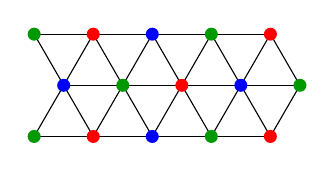
\begin{tikzpicture}[scale=0.75]
  \foreach \j in {0,1,2} \draw ({0.5*mod(\j,2)},{0.866*\j}) -- ++(4,0);
  \foreach \i in {0,...,4} {\draw (\i,0) -- ++(60:1) -- ++(120:1);}
  \foreach \i in {1,...,4} {\draw (\i,0) -- ++(120:1) -- ++(60:1);}
  \foreach \j in {0,1,2} \foreach \i in {0,...,4} {
    \pgfmathtruncatemacro{\c}{mod(\i-floor(\j/2)-\j+30,3)}
    \pgfmathsetmacro{\xx}{\i+0.5*mod(\j,2)}
    \ifnum\c=0 \fill[green!60!black] (\xx,{0.866*\j}) circle (0.11);\fi
    \ifnum\c=1 \fill[red] (\xx,{0.866*\j}) circle (0.11);\fi
    \ifnum\c=2 \fill[blue] (\xx,{0.866*\j}) circle (0.11);\fi
  }
\end{tikzpicture}
\diagramcaption{A proper 3-coloring of a section of the triangular lattice with free boundary conditions.}\label{fig:tri3col}
\end{diagram}

\subsection{Planar duality}

E.g.\ let $G = C_3 = K_3$. The triangle has two faces, the interior and the exterior, so its dual has two vertices, joined by one
edge for each of the three edges of the triangle: $C_3^*$ is the ``fat link'' $FL_3$, where $FL_n$ denotes two vertices joined by
$n$ edges.

\begin{diagram}
\begin{tikzpicture}[scale=0.9]
  \coordinate (A) at (0,0); \coordinate (B) at (1.6,0); \coordinate (Cc) at (0.8,1.3);
  \draw (A) -- (B) -- (Cc) -- cycle; \foreach \p in {A,B,Cc} \node[gv] at (\p) {};
  \node[red] (in) at (0.8,0.45) {$\times$}; \node[red] (out) at (-0.6,1.2) {$\times$};
  \draw[red] (in) -- (out);
  \draw[red] (in) .. controls (1.6,0.9) and (1.4,1.9) .. (0.2,1.9) .. controls (-0.4,1.9) and (-0.7,1.5) .. (out);
  \draw[red] (in) .. controls (0.9,-0.6) and (-0.6,-0.6) .. (-0.9,0.3) .. controls (-1.0,0.7) and (-0.9,1.0) .. (out);
  \node at (2.6,0.65) {so};
  \begin{scope}[xshift=4cm,yshift=0.65cm]
    \node[anchor=east] at (-0.2,0) {$C_3^*$:};
    \node[gv] (p) at (0,0) {}; \node[gv] (q) at (1.6,0) {};
    \draw (p) -- (q); \draw (p) .. controls (0.5,0.55) and (1.1,0.55) .. (q); \draw (p) .. controls (0.5,-0.55) and (1.1,-0.55) .. (q);
    \node[anchor=west] at (1.9,0) {$= FL_3$, ``fat link''};
  \end{scope}
\end{tikzpicture}
\diagramcaption{The planar dual of the triangle $C_3$: one dual vertex ($\times$) inside the triangle and one outside, joined by
three edges.}
\end{diagram}

A lattice example: $(\Lambda_{tri})^* = \Lambda_{hc}$, where tri = triangular lattice and hc = honeycomb lattice. The faces of the
triangular lattice become the vertices of the honeycomb lattice (see Figure~\ref{fig:duality}, read from right to left).

\subsection{The deletion--contraction relation}

DCR = deletion--contraction relation for the chromatic polynomial ($T = 0$ Potts antiferromagnet): consider a graph $G$ and an
edge $e$ in $G$; then
\begin{equation}
  P(G,q) = P(G-e,q) - P(G/e,q),
\end{equation}
where $G-e$ is the graph with $e$ deleted and $G/e$ is the graph with $e$ deleted and the vertices that had been connected via
$e$ contracted (to become a single vertex).

\paragraph{Proof.} We will prove the equivalent relation
\begin{equation}
  P(G-e,q) = P(G,q) + P(G/e,q).
\end{equation}
Consider the proper $q$-colorings of $G-e$. These consist of two classes: (i) colorings with $q(v_i)\ne q(v_j)$, which are
enumerated by $P(G,q)$, since the edge $e$ enforces this condition, and (ii) colorings with $q(v_i) = q(v_j)$; these are
enumerated by $P(G/e,q)$, where we delete $e$ and identify $v_i = v_j$.

\begin{diagram}
\begin{tikzpicture}[scale=0.9]
  \newcommand{\blob}[1]{\draw[pattern=north east lines] (#1) ellipse (0.45 and 0.25);}
  \blob{0,0} \node[gv] (a) at (-0.25,0.7) {}; \node[gv] (b) at (0.25,0.7) {};
  \draw (a) -- (-0.2,0.2); \draw (b) -- (0.2,0.2);
  \node[left,font=\scriptsize] at (-0.25,0.75) {$v_i$}; \node[right,font=\scriptsize] at (0.25,0.75) {$v_j$};
  \node[font=\small] at (0,-0.6) {$G-e$};
  \begin{scope}[xshift=3cm]
    \blob{0,0} \node[gv] (a) at (-0.25,0.7) {}; \node[gv] (b) at (0.25,0.7) {};
    \draw (a) -- (-0.2,0.2); \draw (b) -- (0.2,0.2); \draw (a) -- node[above,font=\scriptsize] {$e$} (b);
    \node[left,font=\scriptsize] at (-0.25,0.75) {$v_i$}; \node[right,font=\scriptsize] at (0.25,0.75) {$v_j$};
    \node[font=\small] at (0,-0.6) {$G$};
  \end{scope}
  \begin{scope}[xshift=6cm]
    \blob{0,0} \node[gv] (a) at (0,0.75) {}; \draw (a) -- (-0.2,0.2); \draw (a) -- (0.2,0.2);
    \node[right,font=\scriptsize] at (0.05,0.8) {$v_i = v_j$};
    \node[font=\small] at (0,-0.6) {$G/e$};
  \end{scope}
\end{tikzpicture}
\diagramcaption{The graphs $G-e$, $G$ and $G/e$ near the edge $e$; the shaded region is the rest of the graph.}
\end{diagram}

E.g.\ for the single edge $K_2$:
\begin{equation}
  P(K_2,q) = P(E_2,q) - P(E_1,q):\qquad q(q-1) = q^2-q .
\end{equation}

N.B.: the chromatic polynomial of a graph in which two vertices are connected by more than one edge is the same as the chromatic
polynomial where they are connected by a single edge. For example, $P(C_2,q) = P(K_2,q)$.

Another example: apply the DCR to one edge of the triangle (marking the edge that is deleted):
\begin{equation}
  P(K_3,q) = P(L_3,q) - P(C_2,q),\qquad
  q(q-1)(q-2):\quad q(q-1)^2 - q(q-1) = q(q-1)(q-2),
\end{equation}
using $P(C_2,q) = P(K_2,q) = q(q-1)$.

% Source: Lecture9.pdf, pages 1-5 (page 6 is blank).
\lecture{9}

We discuss Potts models further here, including an interesting application of Potts
antiferromagnets.

\subsection{Chromatic polynomials and ground-state entropy}
\subsubsection*{Chromatic polynomials from deletion--contraction}

Recall from the previous lecture that, with $v = e^{K_P}-1$,
\begin{equation}
  Z(G,q,v=-1) = P(G,q),
\end{equation}
i.e.\ $Z$ of the zero-temperature Potts antiferromagnet (AFM) on a graph $G$ is precisely the
chromatic polynomial of $G$, enumerating the number of proper $q$-colorings of the vertices of
$G$ with $q$ colors.

The deletion--contraction relation (DCR) provides a way to calculate $P(G,q)$ for any $G$:
\begin{equation}
  P(G,q) = P(G-e,q) - P(G/e,q).
\end{equation}
This can be used iteratively, and at each step, the graphs on the RHS, $G-e$ and $G/e$, involve
one less edge. Hence eventually one is left with $E_n$, for which one has $P(E_n,q) = q^n$.

Example: we previously calculated $Z(C_n,q,v) = (q+v)^n + (q-1)v^n$, so, as a special case,
\begin{equation}
  P(C_n,q) = Z(C_n,q,v=-1) = (q-1)^n + (q-1)(-1)^n .
\end{equation}
Now let us see how this can be derived directly without going through the more complicated
$Z(C_n,q,v)$. Recall that $P(K_3,q) = q(q-1)(q-2)$. Use the DCR to calculate $P(C_4,q)$,
marking the edge to be deleted with a cross:
\begin{equation}
  P(C_4,q) = P(T_4,q) - P(K_3,q),\qquad K_3 = C_3 ,
\end{equation}
since deleting an edge of the square $C_4$ leaves a path (a tree $T_4$), and contracting it
leaves a triangle.

\paragraph{Lemma.} Let $T_n$ be a tree graph with $n$ vertices. Then
$P(T_n,q) = q(q-1)^{n-1}$.

E.g.\ take one example of $T_5$: a path $v_1v_2v_4v_5$ with a vertex $v_3$ attached to $v_2$.
We can pick one of the end vertices and assign any of the $q$ colors to it; let's take $v_1$.
Next, we go on to the adjacent vertex $v_2$; we can use any of the other $q-1$ colors for this
vertex. Next, we can independently assign any of the other $q-1$ colors different from
$q(v_2)$ to $q(v_3)$ and $q(v_4)$. Note that $q(v_1)$ may be equal to $q(v_3)$ or to $q(v_4)$,
since $v_1$ is not adjacent to $v_3$ or $v_4$, and also note that $q(v_3)$ may be equal to
$q(v_4)$, since $v_3$ and $v_4$ are not adjacent. Then one can choose $q(v_5)$ from $q-1$
colors, since the only constraint on this choice is that $q(v_5)\ne q(v_4)$. So
$P(T_5,q) = q(q-1)^4$. Generalizing this, $P(T_n,q) = q(q-1)^{n-1}$.

Now substitute:
\begin{align}
  P(C_4,q) &= P(T_4,q) - P(K_3,q) = q(q-1)^3 - q(q-1)(q-2)\nonumber\\
           &= q(q-1)\left[(q-1)^2-(q-2)\right]\nonumber\\
           &= q(q-1)\left[q^2-3q+3\right] = (q-1)^4 + (q-1)(-1)^4 ,
\end{align}
using $(q-1)^2-(q-2) = q^2-2q+1-q+2 = q^2-3q+3$.

Next proceed inductively:
\begin{equation}
  P(C_5,q) = P(T_5,q) - P(C_4,q);
\end{equation}
we have calculated both of these, so we get $P(C_5,q)$. Etc.:
\begin{equation}
  P(C_n,q) = P(T_n,q) - P(C_{n-1},q)
\end{equation}
$\Rightarrow$ the general result for $P(C_n,q)$ by iterative use of the DCR.

Recall
\begin{equation}
  Z(G,q,v) = \sum_{G'\subseteq G}q^{k(G')}v^{e(G')}
\end{equation}
$\Rightarrow$
\begin{align*}
  \max\deg_q(Z) &= k(E_n) = n(G); & \max\deg_v(Z) &= e(G);\\
  \min\deg_q(Z) &= k(G) = 1; & \min\deg_v(Z) &= e(E_n) = 0 .
\end{align*}
Since $P(G,q) = Z(G,q,v=-1)$, $\Rightarrow\max\deg_q(P) = n(G)$, since $k(E_n)$ does not
depend on $v$; and $\min\deg_q(P) = 1$.

\subsubsection*{Ground-state entropy of the Potts antiferromagnet}

Next, apply these methods to derive an important result in stat.\ mech.\ and thermodynamics.
Consider the $q$-state Potts AFM with $H = 0$ on a bipartite graph,
$G_{\text{bip.}} = G_1\oplus G_2$. We will derive a lower bound on
$Z(G_{\text{bip.}},q,v=-1) = P(G_{\text{bip.}},q)$, the $T = 0$ Potts AFM. A lower bound on
$P(G_{\text{bip.}},q)$ is obtained by assigning one color to all vertices $v_i\in G_1$. This can
be done in any of $q$ ways. Then, independently for each vertex $v_i\in G_2$, we can assign a
color from the remaining set of $q-1$ colors. There are $\frac n2$ vertices in $G_1$ and
$\frac n2$ vertices in $G_2$. So
\begin{equation}
  P(G_{\text{bip.}},q)\ge q(q-1)^{n/2},\qquad\text{where } n = n(G_{\text{bip.}}).
\end{equation}

\begin{diagram}
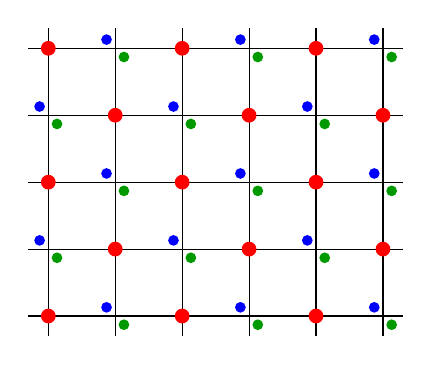
\begin{tikzpicture}[scale=0.85]
  \foreach \x in {0,...,5} \draw (\x,-0.3) -- (\x,4.3);
  \foreach \y in {0,...,4} \draw (-0.3,\y) -- (5.3,\y);
  \foreach \x in {0,...,5} \foreach \y in {0,...,4} {
    \pgfmathtruncatemacro{\prty}{mod(\x+\y,2)}
    \ifnum\prty=0
      \fill[red] (\x,\y) circle (0.11);
    \else
      \fill[blue] (\x-0.13,\y+0.13) circle (0.08);
      \fill[green!60!black] (\x+0.13,\y-0.13) circle (0.08);
    \fi}
\end{tikzpicture}
\diagramcaption{A section of the square lattice with $q = 3$ (red, green, blue). Red is
assigned to all $v_i\in G_1$; then for each $v_j\in G_2$ we can independently choose the color to
be either of the $q-1 = 2$ remaining colors, green or blue. So here
$P(G,3)\ge 3\cdot 2^{n/2} = 3\cdot 2^{15}$, since $n = 30$.}
\end{diagram}

In the general-$q$ case, all of these color assignments (spin states) minimize the energy of the
$q$-state Potts AFM, i.e.\ they are all degenerate ground states of the model.

Given that $Z(G_{\text{bip.}},q,v=-1)\ge q(q-1)^{n/2}$, this means that the $q$-state Potts AFM
(with $H = 0$, zero external magnetic field) has at least this much ground-state degeneracy for
$q\ge 3$. The ground-state degeneracy per site in the thermodynamic limit on a graph $G$ (say
$G$ = lattice $\Lambda$) is, for the Potts AFM,
\begin{equation}
  W(\Lambda,q) = \lim_{n\to\infty}\left[Z(\Lambda,q,v=-1)\right]^{1/n}
              = \lim_{n\to\infty}\left[P(\Lambda,q)\right]^{1/n},
\end{equation}
and the corresponding ground-state entropy per site $\bar S_0$ is
\begin{equation}
  \bar S_0 = \kB\ln W .
\end{equation}
So for the $q$-state Potts AFM on $\Lambda_{\text{bip.}}$,
\begin{equation}
  W(\Lambda_{\text{bip.}},q)_{\text{Potts AFM}}\ge\lim_{n\to\infty}\left[q(q-1)^{n/2}\right]^{1/n}\ge(q-1)^{1/2}
\end{equation}
(using $\lim_{n\to\infty}q^{1/n} = 1$ for $q\ne 0$), and hence
\begin{equation}
  \bar S_0(\Lambda_{\text{bip.}},q)_{\text{Potts AFM}}\ge\frac{\kB}{2}\ln(q-1)>0\quad\text{for } q\ge 3,
\end{equation}
i.e.\ the entropy per site of the $q$-state Potts AFM with $q\ge 3$ is nonzero. This is a
counterexample to the so-called Third ``Law'' of Thermodynamics, which states that
$\bar S_0 = 0$. The fact that this ``law'' has exceptions is well known in stat.\ mech.\ but is
not usually mentioned in elementary physics books.

\subsubsection*{Residual entropy of ice}

Ice is a physical example of nonzero ground state entropy (called $T = 0$ residual entropy in
chemistry). Recall that ice is a hydrogen-bonded molecular crystal and (at $p\sim 1$~atm,
$T\lesssim 0^\circ$C) has a wurtzite crystal structure with tetragonal bonding. On each hydrogen
bond one has an electric dipole; indicate the direction of the electric dipole with an arrow.

Because the bonding is tetragonal, we can represent each oxygen atom as a vertex with degree 4.
Each oxygen atom has 2 hydrogens bonded to it, hence 2 electric dipoles pointing in and 2
electric dipoles pointing out. We represent these as arrows
($\leftarrow,\uparrow,\rightarrow,\downarrow$). The bond angles are not $90^\circ$ and the
crystal structure is not 2-dimensional, but our diagram for a given oxygen atom (vertex with 4
bonds) correctly represents the physics. The Slater Rule, also called the requirement of local
electric neutrality, stipulates that 2 of the 4 arrows must point outward and the other 2
inward. The total number of arrow configurations at each vertex is $2^4 = 16$, but only
$\binom42 = 6$ of these satisfy the constraint of local electric neutrality, where
$\binom ab = \frac{a!}{b!(a-b)!}$.

\begin{diagram}
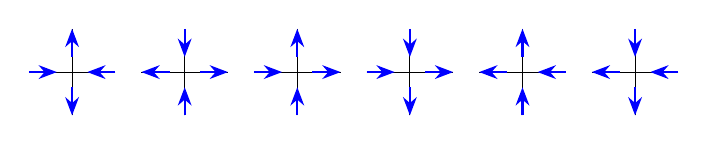
\begin{tikzpicture}[scale=0.55,>=Stealth]
  % each entry: left, right, down, up arrows; 1 = pointing toward the center
  \foreach \n/\l/\r/\d/\u in {0/1/1/0/0, 1/0/0/1/1, 2/1/0/1/0, 3/1/0/0/1, 4/0/1/1/0, 5/0/1/0/1} {
    \begin{scope}[xshift=2.6*\n cm]
      \draw (-1,0) -- (1,0); \draw (0,-1) -- (0,1);
      \ifnum\l=1 \draw[->,blue,thick] (-1,0) -- (-0.35,0); \else \draw[->,blue,thick] (-0.35,0) -- (-1,0); \fi
      \ifnum\r=1 \draw[->,blue,thick] (1,0) -- (0.35,0); \else \draw[->,blue,thick] (0.35,0) -- (1,0); \fi
      \ifnum\d=1 \draw[->,blue,thick] (0,-1) -- (0,-0.35); \else \draw[->,blue,thick] (0,-0.35) -- (0,-1); \fi
      \ifnum\u=1 \draw[->,blue,thick] (0,1) -- (0,0.35); \else \draw[->,blue,thick] (0,0.35) -- (0,1); \fi
    \end{scope}}
\end{tikzpicture}
\diagramcaption{The $\binom42 = 6$ arrow configurations at a vertex allowed by local electric
neutrality (two arrows in, two out). The other 10 arrow configurations, e.g.\ four in or three
in and one out, are forbidden.}
\end{diagram}

The residual entropy of H$_2$O ice is measured to be
$S_0 = 0.82\ \frac{\text{cal}}{\text{mole}\cdot\text{K}}$, i.e.\ (using
$R = N_{\text{Avog.}}\kB = 1.99\ \frac{\text{cal}}{\text{K}\cdot\text{mole}}$) $S_0 = 0.41R$, so
the residual entropy per molecule is $S_0 = 0.41\kB$, so, from $S_0 = \kB\ln W$, i.e.\
$W = e^{S_0/\kB} = e^{0.41} = 1.5$.

Linus Pauling (who was awarded two Nobel Prizes, in Chemistry and Peace) developed a simple
model that yields a very good approximation to this measured value of $\bar S_0$: assume that we
can approximate the total ground state degeneracy (number of g.s.\ configurations of the arrows
on the bonds) as the total number, $2^{e(\Lambda)}$, times the factor arising from the
constraint of local electric neutrality at each vertex of the crystal lattice (i.e.\ each oxygen
atom), namely $\frac{6}{2^4} = \frac38$. Then
\begin{equation}
  Z\simeq 2^{e(\Lambda)}\left(\frac38\right)^{n(\Lambda)}.
\end{equation}
Now $e(\Lambda) = \frac{\Delta}{2}n(\Lambda) = 2n(\Lambda)$ since $\Delta = 4$, so
\begin{equation}
  Z\simeq\left(4\cdot\frac38\right)^{n(\Lambda)} = \left(\frac32\right)^{n(\Lambda)},
  \qquad\text{so}\quad W = \lim_{n(\Lambda)\to\infty}Z^{1/n(\Lambda)} = \frac32 = 1.5 .
\end{equation}
This agrees very well with the measured value of the residual entropy of ice.

References (measurements):
\begin{itemize}
  \item W.F.~Giauque and M.F.~Ashley, Phys.\ Rev.\ \textbf{43}, 81 (1933);
  \item W.F.~Giauque and E.L.~Stout, J.\ Am.\ Chem.\ Soc.\ \textbf{58}, 1144 (1936);
  \item L.~Pauling, \emph{The Nature of the Chemical Bond} (book), p.~467 (1960).
\end{itemize}
Later there have been studies of ``vertex models'' in stat.\ mech.\ as models of ferroelectric
materials, which exhibit a net electric polarization at sufficiently low temperature (e.g.\
KH$_2$PO$_4$, potassium dihydrogen phosphate).

Note that a nonzero ground state entropy results if the actual g.s.\ degeneracy grows like $c^n$
for $c>1$, i.e.\ \#~configurations $\sim c^n$, so $W = c$, $S_0 = \kB\ln W = \kB\ln c$. We have
given two different examples of this phenomenon:
\begin{enumerate}
  \item the $q$-state Potts AF on a bipartite lattice (sq, hc, sc, etc.) for $q\ge 3$, where we
    derived a lower bound on $S_0$ (further calculations give actual estimates of $S_0$ as a
    function of $q$ and $\Lambda_{\text{bip.}}$);
  \item ice and the Pauling model for $S_0$.
\end{enumerate}

\subsubsection*{Frustration}

An important property of both of these examples is that they do \emph{not} involve
frustration. Recall that frustration occurs if the interactions cannot minimize the internal
energy. E.g.:
\begin{enumerate}
  \item An antiferromagnetic spin model in a (uniform) external magnetic field, since the
    spin--spin interaction prefers staggered magnetic ordering, while the external magnetic field
    favors (uniform) magnetic ordering.
  \item An antiferromagnetic spin model on certain non-bipartite lattices, such as the
    triangular lattice. One can see this by considering spin states on a single triangle of the
    lattice; say the spin $\sigma_1$ at vertex 1 is $+$. Then to minimize the interaction energy
    on bonds $e_{12}$ and $e_{13}$ the spins at vertices 2 and 3 should be $-$. But that
    conflicts with the minimization of the spin--spin interaction energy on bond $e_{23}$; with
    this set of spin states,
    \begin{equation}
      \Ham = -J\sum_{e_{ij}}\sigma_i\sigma_j = +|J|\sum_{e_{ij}}\sigma_i\sigma_j
           = |J|(\sigma_1\sigma_2+\sigma_2\sigma_3+\sigma_3\sigma_1) = |J|(-1+1-1) = -|J| .
    \end{equation}
\end{enumerate}
In contrast the ferromagnet can achieve a lower energy with all of the spin--spin interactions
taking their preferred values: with all spins $+$ or all spins $-$,
$\Ham = -J\sum_{e_{ij}}\sigma_i\sigma_j = -3J$.

\begin{diagram}
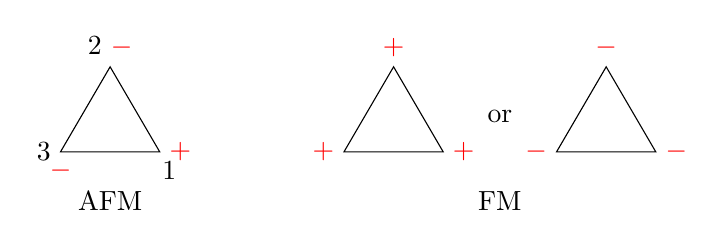
\begin{tikzpicture}[scale=0.9]
  \draw (0,0) -- (1.4,0) -- (0.7,1.2) -- cycle;
  \node[red,right] at (1.4,0) {$+$}; \node[left] at (0,0) {$3$}; \node[red,below] at (0,0) {$-$};
  \node[above] at (0.7,1.2) {$2\ {\color{red}-}$}; \node[below right] at (1.3,0) {$1$};
  \node at (0.7,-0.7) {AFM};
  \begin{scope}[xshift=4cm]
    \draw (0,0) -- (1.4,0) -- (0.7,1.2) -- cycle;
    \node[red,right] at (1.4,0) {$+$}; \node[red,left] at (0,0) {$+$}; \node[red,above] at (0.7,1.2) {$+$};
    \node at (2.2,0.5) {or};
    \begin{scope}[xshift=3cm]
      \draw (0,0) -- (1.4,0) -- (0.7,1.2) -- cycle;
      \node[red,right] at (1.4,0) {$-$}; \node[red,left] at (0,0) {$-$}; \node[red,above] at (0.7,1.2) {$-$};
    \end{scope}
    \node at (2.2,-0.7) {FM};
  \end{scope}
\end{tikzpicture}
\diagramcaption{A frustrated triangle for the Ising AFM, and the two FM ground states.}
\end{diagram}

As we will discuss later, this frustration in the Ising AFM on the triangular lattice drives
$T_c\to 0$.

Another example of a frustrated spin model is a ``spin glass'', where, e.g., the couplings
$J_{ij}$ have different signs on different bonds $e_{ij}$, with some being positive, favoring FM
ordering, and others being negative, favoring AFM ordering. Example: the Ising spin glass,
\begin{equation}
  \Ham = -\sum_{\{e_{ij}\}}\sigma_iJ_{ij}\sigma_j ,
\end{equation}
with the $J_{ij}$ random, distributed with equal probability $>0$ or $<0$: with probability
$\frac12$ for either sign, $J_{ij} = J$ or $-J$; or with a distribution $P(J_{ij})$ peaked
around $\pm J$, or a single broad distribution centered on zero, or a broad distribution with
peaks near $\pm J$.

\begin{diagram}
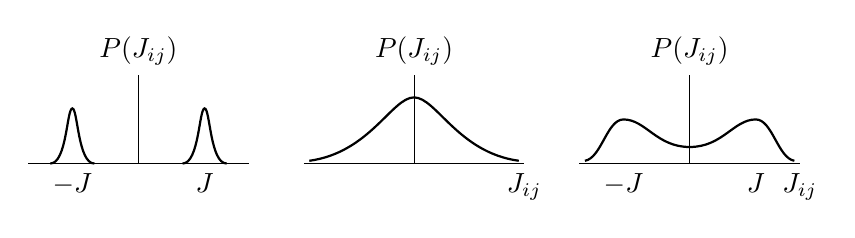
\begin{tikzpicture}[scale=0.7]
  \draw (-2,0) -- (2,0); \draw (0,0) -- (0,1.6) node[above] {$P(J_{ij})$};
  \draw[thick] (-1.6,0) .. controls (-1.3,0) and (-1.3,1) .. (-1.2,1) .. controls (-1.1,1) and (-1.1,0) .. (-0.8,0);
  \draw[thick] (0.8,0) .. controls (1.1,0) and (1.1,1) .. (1.2,1) .. controls (1.3,1) and (1.3,0) .. (1.6,0);
  \node[below] at (-1.2,0) {$-J$}; \node[below] at (1.2,0) {$J$};
  \begin{scope}[xshift=5cm]
    \draw (-2,0) -- (2,0) node[below] {$J_{ij}$}; \draw (0,0) -- (0,1.6) node[above] {$P(J_{ij})$};
    \draw[thick] (-1.9,0.05) .. controls (-0.8,0.2) and (-0.4,1.2) .. (0,1.2) .. controls (0.4,1.2) and (0.8,0.2) .. (1.9,0.05);
  \end{scope}
  \begin{scope}[xshift=10cm]
    \draw (-2,0) -- (2,0) node[below] {$J_{ij}$}; \draw (0,0) -- (0,1.6) node[above] {$P(J_{ij})$};
    \draw[thick] (-1.9,0.05) .. controls (-1.6,0.1) and (-1.5,0.8) .. (-1.2,0.8) .. controls (-0.8,0.8) and (-0.6,0.3) .. (0,0.3)
       .. controls (0.6,0.3) and (0.8,0.8) .. (1.2,0.8) .. controls (1.5,0.8) and (1.6,0.1) .. (1.9,0.05);
    \node[below] at (-1.2,0) {$-J$}; \node[below] at (1.2,0) {$J$};
  \end{scope}
\end{tikzpicture}
\diagramcaption{Possible distributions of the random couplings $J_{ij}$ in an Ising spin glass.}
\end{diagram}

\section{Landau--Ginzburg and mean field theory}
% Source: Lecture10.pdf, pages 1-7. The file has no lecture heading.
\lecture{10}
\subsection{Landau--Ginzburg approach to critical phenomena}

The Landau--Ginzburg (LG) approach to critical phenomena is based on an expansion of the
Helmholtz free energy around the critical temperature $T_c$. For definiteness, we will use
magnetic variables, and write the Helmholtz free energy as $A(T,M)$; the corresponding results for
a liquid--gas phase transition with $A(T,V)$ are obvious.

The LG approach is approximate, and the LG values of critical exponents differ from
experimentally measured values. But nevertheless, the LG approach is useful as a general way to
obtain critical exponents. Later, we will discuss the mean field theory (MFT) approach to phase
transitions. The LG values of critical exponents are equal to the MFT values. In both cases, these
approximations neglect fluctuations. LG theory does not make reference to the dimensionality of the
space or to the symmetry group of the Hamiltonian, $\Ham$. Since experimentally the critical
exponents do depend on the spatial dimension $d$ and the symmetry group of $\Ham$, it is clear that
the LG formalism is only approximate.

LG: write
\begin{equation}
  A(T,M) = \sum_{n=2}^\infty L_n(T)M^n,
\end{equation}
where $M$ = magnetization (e.g.\ $M = \ev{\sigma}$ for the Ising model). (We can drop the $n = 0$
term for our calculations here involving derivatives with respect to $M$.) Since $A(T,M)$ does not
depend on $\sgn(M)$, only even $n$ contribute to this sum. For a continuous phase transition, only
the lowest-order terms in the expansion are important near $T_c$, where $M$ is small. For a
bicritical point we can keep just the $M^2$ and $M^4$ terms:
\begin{equation}
  A(T,M) = L_2(T)M^2 + L_4(T)M^4 + \Order(M^6).
\end{equation}
Next, expand the $L_n(T)$, $n = 2,4$:
\begin{equation}
  L_n(T) = \sum_{k=0}^\infty\ell_{n,k}(T-T_c)^k .
\end{equation}
To fit the dependence of $M$ on $T$, set $\ell_{2,0} = 0$. For boundedness of the Helmholtz energy
as a function of $M$, set $\ell_{4,0}>0$. Then, to leading order, near $T = T_c$,
\begin{equation}
  A(T,M) = \ell_{2,1}(T-T_c)M^2 + \ell_{4,0}M^4 + \ldots
\end{equation}
(higher orders in powers of $M^2$ and powers of $T-T_c$); set $\ell_{2,1}>0$ to agree with the
physical behavior of $M$.

\begin{diagram}
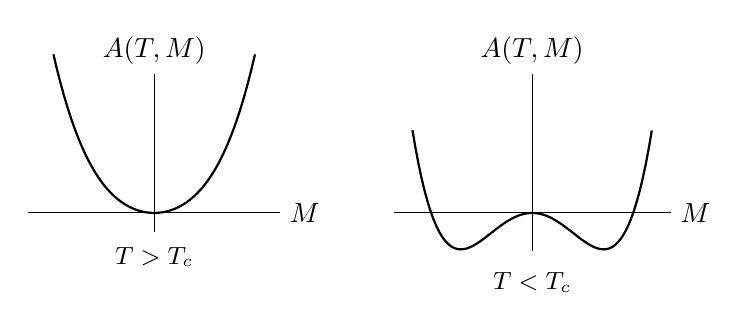
\begin{tikzpicture}[scale=0.8]
  \draw (-2,0) -- (2,0) node[right] {$M$}; \draw (0,-0.3) -- (0,2.2) node[above] {$A(T,M)$};
  \draw[thick,domain=-1.6:1.6,samples=60] plot (\x,{0.6*\x*\x+0.15*\x*\x*\x*\x});
  \node[font=\small] at (0,-0.7) {$T>T_c$};
  \begin{scope}[xshift=6cm]
  \draw (-2.2,0) -- (2.2,0) node[right] {$M$}; \draw (0,-0.6) -- (0,2.2) node[above] {$A(T,M)$};
  \draw[thick,domain=-1.9:1.9,samples=80] plot (\x,{-0.9*\x*\x+0.35*\x*\x*\x*\x});
  \node[font=\small] at (0,-1.1) {$T<T_c$};
  \end{scope}
\end{tikzpicture}
\diagramcaption{Graphically: for $T>T_c$ the minimum of the Helmholtz free energy is at $M = 0$,
so there is no magnetization. For $T<T_c$ the minima of $A(T,M)$ are at nonzero $\pm M$,
indicating nonzero magnetization.}
\end{diagram}

This results because $L_2(T)$ reverses sign as $T$ passes through $T_c$.

Calculate the position of the minimum of $A$: this occurs where $\partial A/\partial M = 0$ with
$\partial^2A/\partial M^2>0$:
\begin{equation}
  \pder{A}{M} = 2\ell_{2,1}(T-T_c)M + 4\ell_{4,0}M^3 = 2M\left[\ell_{2,1}(T-T_c) + 2\ell_{4,0}M^2\right].
\end{equation}
For $T>T_c$, the minimum of $A$ is at $M = 0$. For $T<T_c$, the minimum of $A$ is at
\begin{equation}
  M = \pm\left[\frac{\ell_{2,1}(T_c-T)}{2\ell_{4,0}}\right]^{1/2}.
\end{equation}
The sign of $\partial^2A/\partial M^2$ at these points:
\begin{align}
  \frac{\partial^2A}{\partial M^2} &= 2\ell_{2,1}(T-T_c) + 12\ell_{4,0}M^2
    = 2\ell_{2,1}(T-T_c) + 12\ell_{4,0}\left(-\frac{\ell_{2,1}(T-T_c)}{2\ell_{4,0}}\right)\nonumber\\
  &= 2\ell_{2,1}(T-T_c) - 6\ell_{2,1}(T-T_c) = 4\ell_{2,1}(T_c-T)>0\quad\text{for } T<T_c
\end{align}
(and $=2\ell_{2,1}(T-T_c)$ for $T>T_c$, where $M = 0$). This shows that these are minima of $A$,
which is clear from the graphs.

Recall the definition of the critical exponent $\beta$: $M\propto(T_c-T)^\beta$ as
$T_c-T\to 0^+$, i.e.\ $\ln M = \beta\ln(T_c-T)$,
\begin{equation}
  \beta = \lim_{T\to T_c^-}\frac{\ln M}{\ln(T_c-T)}.
\end{equation}
From our solution for $M$ above, we find
\begin{equation}
  \text{LG:}\quad\boxed{\beta = \frac{1}{2}}.
\end{equation}

Next, calculate the magnetic susceptibility $\chi = \partial M/\partial H$ as $T\to T_c$ and the
corresponding critical exponents:
\begin{equation}
  \chi\propto
  \begin{cases}
    (T-T_c)^{-\gamma} & \text{as } T\to T_c^+\\
    (T_c-T)^{-\gamma'} & \text{as } T\to T_c^- .
  \end{cases}
\end{equation}
Recall $\dd A(T,M) = -S\dd T + H\dd M$, so
\begin{equation}
  H = \left(\pder{A}{M}\right)_T;\qquad \pder{H}{M} = \left(\frac{\partial^2A}{\partial M^2}\right)_T,
  \qquad\text{i.e.}\quad \chi = \left(\pder{M}{H}\right) = \left[\frac{\partial^2A}{\partial M^2}\right]^{-1}.
\end{equation}
Now we calculated $(\partial^2A/\partial M^2)_T$ above: for $T>T_c$, the minimum of $A$ is at
$M = 0$, where $\partial^2A/\partial M^2 = 2\ell_{2,1}(T-T_c)>0$. So as $T\to T_c^+$,
\begin{equation}
  \chi\simeq\frac{1}{2\ell_{2,1}(T-T_c)},\qquad\text{so}\quad\boxed{\gamma = 1}.
\end{equation}
For $T<T_c$, $\partial^2A/\partial M^2 = 4\ell_{2,1}(T_c-T)$ at the minimum of $A$
$\Rightarrow\chi = [4\ell_{2,1}(T_c-T)]^{-1}\Rightarrow\gamma' = 1$.

So the LG approach yields $\beta = 1/2$ and $\gamma = \gamma' = 1$. (Note that the critical
amplitudes for $\chi$ for $T>T_c$ and $T<T_c$ are different:
\begin{equation}
  \chi\sim
  \begin{cases}
    \dfrac{1}{2\ell_{2,1}(T-T_c)} & \text{as } T-T_c\to 0^+\\[8pt]
    \dfrac{1}{4\ell_{2,1}(T_c-T)} & \text{as } T-T_c\to 0^- .)
  \end{cases}
\end{equation}

Next, calculate the LG value for the critical exponent describing the critical isotherm,
$|M|^\delta\sgn(M) = H$ at $T_c$. Take $H>0$, so $M^\delta = H$, i.e.\ $M = H^{1/\delta}$ at $T_c$.
Now from $\dd A(T,M) = -S\dd T + H\dd M$, with $H = (\partial A/\partial M)_T$, recall
$(\partial A/\partial M)_T = 2\ell_{2,1}(T-T_c)M + 4\ell_{4,0}M^3$. Set $T = T_c$; then
\begin{equation}
  \left(\pder{A}{M}\right)_{T=T_c} = 4\ell_{4,0}M^3 = H,\qquad\text{so}\quad
  \text{LG:}\ \boxed{\delta = 3}.
\end{equation}

\begin{diagram}
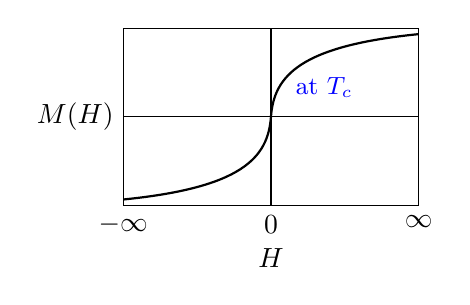
\begin{tikzpicture}[scale=0.75]
  \draw (0,0) rectangle (5,3); \draw (0,1.5) -- (5,1.5); \draw (2.5,0) -- (2.5,3);
  \draw[thick] (0,0.1) .. controls (2,0.3) and (2.45,0.8) .. (2.5,1.5) .. controls (2.55,2.2) and (3,2.7) .. (5,2.9);
  \node[left] at (0,1.5) {$M(H)$};
  \node[below] at (0,0) {$-\infty$}; \node[below] at (2.5,0) {$0$}; \node[below] at (5,0) {$\infty$};
  \node[below=12pt] at (2.5,0) {$H$};
  \node[blue,font=\small] at (3.4,2.0) {at $T_c$};
\end{tikzpicture}
\diagramcaption{The critical isotherm.}
\end{diagram}

The approximate nature of the Landau--Ginzburg formalism is clear from the fact that it is based on
an expansion of the Helmholtz free energy $A(T,M)$ as a function of $M$ and $T$, about $T = T_c$,
$M = 0$. This would be justified if $A(T,M)$ were analytic at this point, but it is not, as is
evident from $M(T)$ and $\chi(T)$.

\begin{diagram}
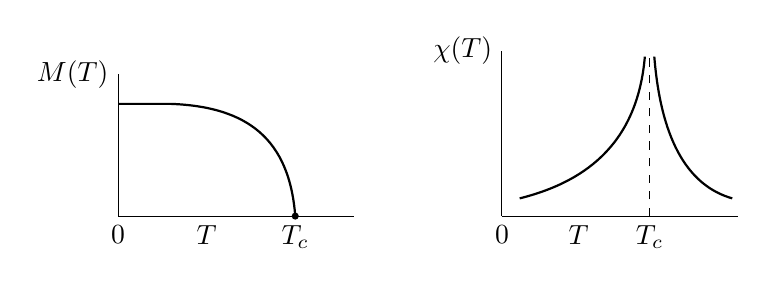
\begin{tikzpicture}[scale=0.75]
  \draw (0,0) -- (4,0); \draw (0,0) -- (0,2.4) node[left] {$M(T)$};
  \draw[thick] (0,1.9) -- (0.9,1.9) .. controls (2.2,1.85) and (2.9,1.3) .. (3,0);
  \fill (3,0) circle (0.06);
  \node[below] at (0,0) {$0$}; \node[below] at (1.5,0) {$T$}; \node[below] at (3,0) {$T_c$};
  \begin{scope}[xshift=6.5cm]
  \draw (0,0) -- (4,0); \draw (0,0) -- (0,2.8) node[left] {$\chi(T)$};
  \draw[dashed] (2.5,0) -- (2.5,2.8);
  \draw[thick] (0.3,0.3) .. controls (1.5,0.6) and (2.3,1.3) .. (2.42,2.7);
  \draw[thick] (2.58,2.7) .. controls (2.7,1.2) and (3.2,0.5) .. (3.9,0.3);
  \node[below] at (0,0) {$0$}; \node[below] at (1.3,0) {$T$}; \node[below] at (2.5,0) {$T_c$};
  \end{scope}
\end{tikzpicture}
\diagramcaption{The magnetization and susceptibility are nonanalytic at $T_c$.}
\end{diagram}

Nevertheless, the LG formalism provides a useful approximate approach to critical behavior.

\subsection{Mean field theory approach to phase transitions}\label{sec:mft}

For definiteness, we discuss MFT using the simplest spin model as an illustration, namely the Ising
model. Then we generalize to other spin models.
\begin{equation}
  Z = \sum_{\{\sigma_i\}}e^{-\beta\Ham},\qquad
  \Ham = -J\sum_{e_{ij}}\sigma_i\sigma_j - H\sum_i\sigma_i,\qquad\beta = \frac{1}{\kB T},
\end{equation}
\begin{equation}
  Z = \sum_{\{\sigma_i\}}e^{K\sum_{e_{ij}}\sigma_i\sigma_j + h\sum_i\sigma_i},
  \qquad\text{where, as before,}\quad K\equiv\beta J,\ h\equiv\beta H .
\end{equation}
What makes the calculation of $Z$ and $f = \lim_{N\to\infty}(1/N)\ln Z$ difficult is the coupled,
many-body (actually infinite in the $N\to\infty$ limit) nature of the problem. MFT simplifies the
problem drastically by approximating the coupled many-body problem by a 1-body problem, assuming
that a given spin $\sigma_0$ interacts with a mean (= average) magnetic field due to all of the other
spins. So the actual $\Ham$ is replaced by
\begin{equation}
  \Ham_{\text{MFT}} = -J\sum_{\text{n.n.}\,i}\sigma_0\sigma_i - H\sigma_0,\qquad\text{i.e.}\quad
  -\beta\Ham_{\text{MFT}} = K\sum_{\text{n.n.}\,i}\sigma_0\sigma_i + h\sigma_0,
\end{equation}
where $\sigma_i = \ev{\sigma_i}$, the mean magnetization $\bar M$, and n.n.\ $i$ = nearest-neighbor
sites $i$ (adjacent vertices in the terminology of graph theory). The physical application is to the
model on a regular lattice with coordination number = vertex degree $\Delta$, with
$\ev{\sigma_i} = \bar M$. So
\begin{equation}
  -\beta\Ham_{\text{MFT}} = K\Delta\sigma_0\bar M + h\sigma_0 = (K\Delta\bar M + h)\sigma_0,
\end{equation}
so for the single site, denoted 0,
\begin{equation}
  Z_{ss,\text{MFT}} = \sum_{\sigma_0=\pm1}e^{(K\Delta\bar M+h)\sigma_0}
  = e^{K\Delta\bar M+h} + e^{-(K\Delta\bar M+h)} = 2\cosh(K\Delta\bar M+h),
\end{equation}
and $Z_{\text{MFT}} = (Z_{ss,\text{MFT}})^N$,
\begin{equation}
  f_{\text{MFT}} = \lim_{N\to\infty}\frac{1}{N}\ln Z_{\text{MFT}} = \ln[Z_{ss,\text{MFT}}]
  = \ln[2\cosh(K\Delta\bar M+h)].
\end{equation}
The Gibbs free energy is $G_{\text{MFT}}(T,H) = -\kB Tf_{\text{MFT}}$, and
\begin{equation}
  \bar M = \pder{f}{h} = \tanh(K\Delta\bar M + h)\quad\text{in MFT}.
\end{equation}
The spontaneous magnetization is
\begin{equation}
  \bar M_{sp} = \lim_{H\to 0}\bar M = \tanh(K\Delta\bar M_{sp}).
\end{equation}
At high temperature, $\beta\to 0$, so the only solution is $\bar M_{sp} = 0$. As $T$ decreases
($\beta$ increases) a nonzero solution first occurs (i.e.\ $\bar M_{sp}$ increases from zero) when,
expanding the tanh, $\bar M_{sp} = K\Delta\bar M_{sp}$, i.e.\ at $K\Delta = 1$,
\begin{equation}
  K_{c,\text{MFT}} = \frac{1}{\Delta}.
\end{equation}
(Here we used the Taylor series expansion $\tanh x\simeq x + \Order(x^3)$ for $x\to 0$.) So the
critical temperature in the MFT approximation is $K_{c,\text{MFT}} = 1/\Delta$, i.e.\
$\beta_{c,\text{MFT}} = 1/(J\Delta) = 1/(\kB T_{c,\text{MFT}})$, so
\begin{equation}
  T_{c,\text{MFT}} = \frac{J\Delta}{\kB}.
\end{equation}
Note the dependence on the lattice coordination number, but no explicit dependence on lattice
dimensionality. Thus the MFT prediction for $T_c$ for the Ising model on the triangular lattice,
which is 2-dimensional, is the same as the prediction for $T_c$ for the Ising model on the simple
cubic lattice, which is 3-dimensional, since both have the same coordination number, $\Delta = 6$.
In reality, these $T_c$ values are not equal. This shows one deficiency in MFT.

Furthermore, MFT neglects fluctuations, which tend to disorder the spins, so one must actually make
$T$ \emph{lower} than the MFT prediction, $(T_c)_{\text{MFT}}$, in order for the phase transition to
occur and for a nonzero spontaneous magnetization (LRO). For example, we will later derive
$K_{c,sq}$, the critical $K_c$ for the Ising model on the square lattice. This is
\begin{equation}
  K_{c,sq} = \frac{1}{2}\ln(1+\sqrt2) = 0.4407,
\end{equation}
and, with $K = \beta J = J/(\kB T)$, this means that
\begin{equation}
  \kB T_{c,sq} = \frac{2J}{\ln(1+\sqrt2)} = 2.269\,J .
\end{equation}
Compare with $K_{c,\text{MFT}} = 1/\Delta_{sq} = 1/4 = J/(\kB T_{c,\text{MFT}})$
$\Rightarrow\kB T_{c,\text{MFT}} = 4J$. So
\begin{equation}
  \frac{T_{c,sq}}{T_{c,\text{MFT}}} = \frac{K_{c,\text{MFT}}}{K_{c,sq}}
  = \frac{1/4}{(1/2)\ln(1+\sqrt2)} = \frac{1}{2\ln(1+\sqrt2)} = 0.5673,
\end{equation}
which is $<1$, for the reason given above: the neglect of disordering fluctuations in MFT.

\subsubsection*{Critical exponents in MFT}

Use $\bar M_{sp} = \tanh(K\Delta\bar M_{sp})$ and the expansion
$\tanh x = x - (1/3)x^3 + \Order(x^5)$ as $x\to 0$, so
\begin{equation}
  \bar M_{sp} = K\Delta\bar M_{sp} - \frac{1}{3}(K\Delta\bar M_{sp})^3 + \Order\left((K\Delta\bar M_{sp})^5\right)
\end{equation}
as $T\to T_c^-$, and hence $\bar M_{sp}\to 0$. For $T<T_c$, divide both sides by $\bar M_{sp}$, which
is nonzero:
\begin{align}
  &\Rightarrow 1 = K\Delta - \frac{1}{3}(K\Delta)^3\bar M_{sp}^2 + \Order\left((K\Delta)^5\bar M_{sp}^4\right)
    = K\Delta\left[1-\frac{1}{3}(K\Delta)^2\bar M_{sp}^2+\ldots\right]\nonumber\\
  &\Rightarrow\frac{1}{K\Delta} = 1-\frac{1}{3}(K\Delta)^2\bar M_{sp}^2+\ldots
  \ \Rightarrow\ \bar M_{sp}^2 = \frac{3}{(K\Delta)^2}\left[1-\frac{1}{K\Delta}\right]
  \quad\text{as } T\to T_c^-,
\end{align}
where the $\Order((K\Delta)^5\bar M_{sp}^4)$ term is negligible as $T\to T_c^-$. Then
\begin{equation}
  \bar M_{sp}^2 = \frac{3}{(K\Delta)^2}\left[1-\frac{1}{K\Delta}\right]
  = \frac{3}{(K\Delta)^2}\left[1-\frac{K_c}{K}\right] = \frac{3}{K^3\Delta^2}(K-K_c).
\end{equation}
Now $K-K_c = J(\beta-\beta_c) = (J/\kB)\left(1/T-1/T_c\right) = (J/(\kB TT_c))(T_c-T)$,
so
\begin{equation}
  \bar M_{sp}^2 = \left(\frac{3}{K_c^3\Delta^2}\right)\underbrace{\left(\frac{J}{\kB T_c}\right)}_{K_c}\left(\frac{T_c-T}{T_c}\right)
  = \frac{3}{(K_c\Delta)^2}\left(\frac{T_c-T}{T_c}\right),
\end{equation}
where $3/(K_c\Delta)^2$ is a constant. So $\bar M_{sp}\propto(T_c-T)^{1/2}$ as $T\to T_c^-$, so the
critical exponent is
\begin{equation}
  \boxed{\beta = \frac{1}{2}\ \text{in MFT}}.
\end{equation}

Next, calculate the critical behavior of $\chi$ and the associated exponents $\gamma$, $\gamma'$:
use the basic MFT equation $\bar M = \tanh(K\Delta\bar M + h)$. Now expand for $T$ near $T_c$, using
$\tanh x = x - x^3/3 + \Order(x^5)$ for small $x$, and use
$\bar\chi = \partial M/\partial H = \beta\partial M/\partial h$, so $\beta^{-1}\bar\chi = \partial M/\partial h$:
\begin{equation}
  \bar M = (K\Delta\bar M + h) - \frac{1}{3}(K\Delta\bar M+h)^3+\ldots,\qquad
  (1-K\Delta)\bar M = h - \frac{1}{3}(K\Delta\bar M+h)^3+\ldots
\end{equation}
Let $K\Delta\equiv\kappa$. Then
\begin{equation}
  \Rightarrow\ \bar M = \frac{h}{(1-K\Delta)} - \frac{1}{3(1-K\Delta)}\left[(\kappa\bar M)^3 + 3(\kappa\bar M)^2h + 3(\kappa\bar M)h^2 + h^3\right]+\ldots
\end{equation}
The first term is the leading-order behavior as $T\to T_c$, so $\partial \bar M/\partial h = 1/(1-K\Delta)$:
\begin{equation}
  \beta^{-1}\bar\chi = \frac{1}{1-K\Delta} = \frac{1}{1-K/K_c}\propto\frac{1}{K_c-K}\propto\frac{1}{T-T_c},
\end{equation}
so $\gamma = 1$; similarly, $\gamma' = 1$. The other terms are negligible as $T\to T_c$ (HW).
Similarly, the critical exponent for the critical isotherm is $\delta = 3$.

\subsubsection*{Comparison of \texorpdfstring{$T_{c,\text{MFT}}$}{Tc,MFT} with actual values}

It is of interest to compare the MFT prediction for $T_c$ with the actual values of $T_c$ for 3D
lattices, extending our previous comparison for the square lattice (2D). Consider the simple cubic
(sc) lattice. Analysis of high-$T$ series expansions $\Rightarrow\tanh(K_{c,sc})\simeq 0.21813$
$\Rightarrow K_{c,sc}\simeq 0.22169$, and
\begin{equation}
  \frac{T_{c,sc}}{T_{c,\text{MFT},sc}} = \frac{K_{c,\text{MFT},sc}}{K_{c,sc}} = \frac{1/6}{0.2217}\simeq 0.752 .
\end{equation}
From this comparison, we see that as the dimension (coordination number) increases, the MFT
prediction for $T_c$ becomes more accurate; this ratio was 0.567 for the square lattice.

Let us give another comparison, for the body-centered cubic (bcc) lattice; see the picture in
Figure~\ref{fig:cubic}; $\Delta = 8$ for the bcc lattice. Analysis of high-temperature series
expansions gives $K_{c,bcc} = 0.157407$, so
\begin{equation}
  \frac{T_{c,bcc}}{(T_c)_{\text{MFT},bcc}} = \frac{K_{c,\text{MFT},bcc}}{K_{c,bcc}} = \frac{1/8}{0.157407}\simeq 0.7941 .
\end{equation}
Summary of these comparisons:
\begin{center}
\begin{tabular}{lcc}
  lattice & $T_c/T_{c,\text{MFT}}$ & $\Delta$\\ \hline
  sq & 0.57 & 4\\
  sc & 0.75 & 6\\
  bcc & 0.79 & 8
\end{tabular}
\end{center}
This shows a trend, namely that as $\Delta$ increases, the MFT prediction for $T_c$ becomes more
accurate. An early review is by C.~Domb in the C.~Domb and M.~Green series entitled \emph{Phase
Transitions and Critical Phenomena}; see vol.~3.

% Source: Lecture11.pdf, pages 1-6.
\lecture{11}
\subsubsection*{Mean field theory for an \texorpdfstring{$O(2)$}{O(2)} spin model}

An example of an application of mean field theory to a continuous spin system: consider a spin
model with spins in $S^1$, i.e.\ $\mathbf{S}_i = (\cos\theta_i,\sin\theta_i)$ (normalize
$\mathbf{S}$ so $|\mathbf{S}| = 1$), and
\begin{equation}
  \Ham = -J\sum_{e_{ij}}\mathbf{S}_i\cdot\mathbf{S}_j - \mathbf{H}\cdot\sum_i\mathbf{S}_i .
\end{equation}
The spin--spin interaction is
\begin{equation}
  \mathbf{S}_i\cdot\mathbf{S}_j = \cos\theta_i\cos\theta_j + \sin\theta_i\sin\theta_j = \cos(\theta_i-\theta_j).
\end{equation}
In the absence of an external magnetic field $\mathbf{H}$, the Hamiltonian is invariant under a
global $O(2)$ symmetry group with elements $R(\omega)$ that rotate each spin by the angle $\omega$.
This is clear, since the scalar product $\mathbf{S}_i\cdot\mathbf{S}_j$ is invariant under such
rotations: $\cos(\theta_i-\theta_j)\to\cos((\theta_i+\omega)-(\theta_j+\omega))$. A nonzero external
field breaks this $O(2)$ symmetry explicitly and a nonzero spontaneous magnetization breaks it
spontaneously. The partition function is now the multiple ($N$-fold) integral
\begin{equation}
  Z = \left[\prod_{i=1}^N\int_0^{2\pi}\frac{\dd\theta_i}{2\pi}\right]e^{-\beta\Ham}
    = \left[\prod_{i=1}^N\int_0^{2\pi}\frac{\dd\theta_i}{2\pi}\right]
      e^{K\sum_{e_{ij}}\cos(\theta_i-\theta_j) + h\sum_i\cos\theta_i},
\end{equation}
where we have taken $\mathbf{H}$ to point along the $\hat{\mathbf{x}}$ axis in the $O(2)$ space (just
define $\hat{\mathbf{x}}$ in $O(2)$ space to point along $\mathbf{H}$; no loss of generality).

MFT approximates the partition function by assuming that each spin interacts with a mean field (per
site) $\bar{\mathbf{M}}\equiv\langle\mathbf{M}\rangle$ due to all of the other spins, so the full
partition function reduces to an $N$-fold product of single-site (ss) integrals. Since
$\mathbf{H} = H(1,0)$, the induced $\bar{\mathbf{M}} = \bar M(1,0)$. So for the reference spin
$\mathbf{S}_0$,
\begin{equation}
  \sum_{e_{0j}}\mathbf{S}_0\cdot\ev{\mathbf{S}} = (\cos\theta_0,\sin\theta_0)\cdot\bar M(1,0)\,\Delta
  = (\bar M\cos\theta_0)\,\Delta,
\end{equation}
where $\Delta$ = lattice coordination number, and $Z_{\text{MFT}} = (Z_{ss})^N$, with
\begin{equation}
  Z_{ss} = \int_0^{2\pi}\frac{\dd\theta_0}{2\pi}e^{K\sum_{e_{0j}}\mathbf{S}_0\cdot\ev{\mathbf{S}} + \mathbf{h}\cdot\mathbf{S}_0}
  = \int_0^{2\pi}\frac{\dd\theta_0}{2\pi}e^{(K\Delta\bar M+h)\cos\theta_0},
  \qquad x\equiv K\Delta\bar M + h .
\end{equation}
Now
\begin{equation}
  \int_0^{2\pi}\frac{\dd\theta_0}{2\pi}e^{x\cos\theta_0} = I_0(x),
\end{equation}
where $I_\nu(x)$ is the modified Bessel function of index $\nu$, with series expansion
\begin{equation}
  I_\nu(x) = \sum_{\ell=0}^\infty\frac{(x/2)^{\nu+2\ell}}{\ell!\,\Gamma(\nu+\ell+1)},
\end{equation}
where $\Gamma(y)$ is the Euler $\Gamma$ function: $\Gamma(y+1) = y\Gamma(y)$ and $\Gamma(n) = (n-1)!$
for integer $n$. So
\begin{gather}
  I_0(x) = 1 + \frac{(x/2)^2}{\Gamma(2)} + \Order(x^4) = 1 + \frac{x^2}{4} + \Order(x^4)
  \quad(\Gamma(2) = 1),\nonumber\\
  I_1(x) = \frac{(x/2)}{\Gamma(2)} + \Order(x^3) = \frac{x}{2} + \Order(x^3).
\end{gather}
Another relation is $\dd I_0(x)/\dd x = I_1(x)$. The dimensionless reduced Gibbs free energy in
the MFT approximation is then
\begin{equation}
  f_{\text{MFT}} = \lim_{N\to\infty}\frac{1}{N}\ln Z_{\text{MFT}} = \ln(Z_{ss}) = \ln(I_0(x)) = \ln\left[I_0(K\Delta\bar M+h)\right].
\end{equation}
Calculate $\bar M$:
\begin{equation}
  \bar M = \pder{f}{h} = \pder{}{h}\ln\left[I_0(K\Delta\bar M+h)\right] = \frac{I_1(K\Delta\bar M+h)}{I_0(K\Delta\bar M+h)}.
\end{equation}
The spontaneous magnetization is $\bar M_{sp} = \lim_{h\to 0}\bar M$, so
\begin{equation}
  \bar M_{sp} = \frac{I_1(K\Delta\bar M_{sp})}{I_0(K\Delta\bar M_{sp})}.
\end{equation}
This is the analogue, in this $O(2)$ spin model, of the equation
$\bar M_{sp} = \tanh(K\Delta\bar M_{sp})$ that we derived previously for the Ising model in the MFT
approximation. As before, at high temperature $T$, i.e.\ small $\beta$ and hence small $K = \beta J$,
the only solution is $\bar M_{sp} = 0$. As $T$ decreases, and hence $K$ increases, a nonzero solution
first occurs if RHS $=\bar M_{sp}$, where $|\bar M_{sp}|\ll 1$. So we calculate this by expanding the
Bessel functions for small arguments, using $I_1(x) = x/2 + \Order(x^3)$ and
$I_0(x) = 1 + \Order(x^2)$:
\begin{equation}
  \bar M_{sp} = \frac{K\Delta\bar M_{sp}}{2} + \ldots,
\end{equation}
so a nonzero solution occurs as $K$ is increasing from 0 at $K\Delta = 2$, i.e.
\begin{equation}
  K = K_{c,\text{MFT},O(2)} = \frac{2}{\Delta}.
\end{equation}
Comparing this with the result for Ising, $K_{c,\text{MFT},\text{Ising}} = 1/\Delta$, we see that
\begin{equation}
  \kB T_{c,\text{MFT},O(2)} = \frac{J\Delta}{2}\qquad\text{vs.}\qquad\kB T_{c,\text{MFT},\text{Ising}} = J\Delta .
\end{equation}
So MFT predicts that one must cool a system of $O(2)$ spins to twice as low a temperature to get the
phase transition to the symmetry-broken phase with a spontaneous magnetization as compared with an
Ising spin model on the same lattice. This is physically understandable because the spins in the
$O(2)$ model are ``floppier'' than the spins in the Ising model, so one needs a lower temperature to
get them to have ``long-range order'' (LRO), where ``long'' means infinite.

Thus, MFT yields predictions for $T_c$ that depend on
\begin{enumerate}[label=(\roman*)]
  \item the lattice coordination number (vertex degree) $\Delta$;
  \item intrinsic properties of the dynamical variables, as shown e.g.\ by the comparison of the
    application to the Ising vs.\ $O(2)$ spin models;
  \item because of the neglect of fluctuations in MFT, the true $T_c$ is smaller than the MFT
    prediction.
\end{enumerate}
We showed this quantitatively by comparing the MFT prediction for $T_c$ with the exactly known
$T_c$ for the Ising model on a 2D lattice (the square lattice) and two 3D lattices, sc and bcc. We
saw that the MFT prediction becomes more accurate as the dimension of the lattice increases.

A drastic example of a failure of MFT is for a 1-dimensional lattice. Here, $\Delta = 2$, so MFT
predicts that there will be a phase transition to a ferromagnetic phase at a finite temperature,
e.g.\ $T_c = J\Delta/\kB = 2J/\kB$ for an Ising model. But the Peierls Theorem shows that there is no
nonzero spontaneous magnetization and associated FM LRO at any finite temperature; this only occurs
at $T = 0$. Our exact solution for $\bar M(T,H)$ and $\bar M_{sp} = \lim_{H\to 0}\bar M(T,H)$ showed
this explicitly.

\subsection{Peierls argument in two and more dimensions}

Recall the Peierls Theorem for a 1D spin system, e.g.\ Ising. This showed that a would-be
ferromagnetically ordered state is unstable to the occurrence of a disordering seam (and hence to
multiple such seams), from $\cdots{+}{+}{+}{+}{+}{+}\cdots$ to $\cdots{+}{+}{+}\,|\,{-}{-}{-}\cdots$,
with a seam where the spins flip:
\begin{equation}
  \Delta G = 2J - T\Delta S = 2J - \kB T\ln N,
\end{equation}
since the seam can occur anywhere. As $N\to\infty$, for any $T>0$, the second term dominates, so
the occurrence of this disordering seam lowers the free energy. Only at $T = 0$, where
$\Delta G = \Delta U$, does the seam raise the free energy, and hence only at $T = 0$ does the system
have $\bar M\ne 0$.

We now show how a Peierls-type argument proves that for a discrete spin model in $d\ge 2$
dimensions (without frustration or competing interactions) there is a phase transition to a
low-temperature phase with nonzero spontaneous magnetization. Consider the FM case $J>0$; on a
bipartite lattice there is an isomorphism relating this to the AFM case $J<0$. Consider a
ferromagnetically ordered state, and again analyze $\Delta G$ when one introduces a disordering
seam, e.g.\ on the square lattice.

\begin{diagram}
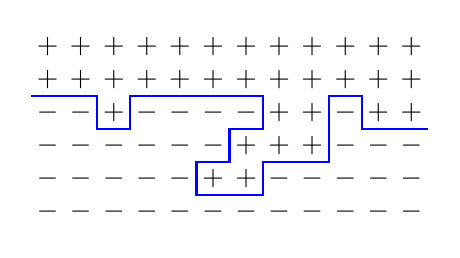
\begin{tikzpicture}[scale=0.42]
  \foreach \r/\row in {
    0/{+,+,+,+,+,+,+,+,+,+,+,+},
    1/{+,+,+,+,+,+,+,+,+,+,+,+},
    2/{-,-,+,-,-,-,-,+,+,-,+,+},
    3/{-,-,-,-,-,-,+,+,+,-,-,-},
    4/{-,-,-,-,-,+,+,-,-,-,-,-},
    5/{-,-,-,-,-,-,-,-,-,-,-,-}} {
    \foreach \s [count=\c] in \row { \node at (\c,-\r) {$\s$}; } }
  \draw[blue,thick] (0.5,-1.5) -- (2.5,-1.5) -- (2.5,-2.5) -- (3.5,-2.5) -- (3.5,-1.5) -- (7.5,-1.5)
     -- (7.5,-2.5) -- (6.5,-2.5) -- (6.5,-3.5) -- (5.5,-3.5) -- (5.5,-4.5) -- (7.5,-4.5) -- (7.5,-3.5)
     -- (9.5,-3.5) -- (9.5,-1.5) -- (10.5,-1.5) -- (10.5,-2.5) -- (12.5,-2.5);
\end{tikzpicture}
\diagramcaption{A disordering seam (blue) in a rectangular section of an $n\times n$ square
lattice, so $N_{\text{tot}} = n^2$. The increase in the internal energy is $(2J)L$, where $L$ is
the length of the seam.}
\end{diagram}

Now make rough estimates of typical lengths $L$ and the entropic term $T\Delta S$ to estimate the
$\Delta G$ due to the seam. Say we start the wall from the left; there are $\sim n$ places where it
can start. At a typical internal site, there are at least 2 ways, and sometimes 3 ways, the seam
can propagate ($\rightarrow\rightarrow$ or $\rightarrow\uparrow$ or $\rightarrow\downarrow$). Let us
denote this number of choices as $c$, where $2\le c\le 3$. Since the seam zigzags, its length
$L>n$; use the estimate $L\simeq\lambda n$. Then the change in the internal energy $U$ due to the
seam is
\begin{equation}
  \Delta U = (2J)L\simeq 2J\lambda n .
\end{equation}
Since the seam can start at any of $n$ positions on the left and since at every step there are $c$
choices of how to proceed, the entropic term is
\begin{equation}
  -T\Delta S\simeq -\kB T\ln(n\cdot c^L) = -\kB T\ln\left(n\cdot e^{\lambda n\ln c}\right)
  = -\kB T\left[\ln n + \lambda n\ln c\right];
\end{equation}
for $n\gg 1$ the term $\propto n$ dominates over the $\ln n$ term, which we can drop. So
\begin{equation}
  \Delta G\simeq 2J\lambda n - \kB T\cdot\lambda n\ln c = \lambda n(2J - \kB T\cdot\ln c),
  \qquad\text{so}\quad \Delta G>0\ \text{if}\ T<\frac{2J}{\kB\ln c}.
\end{equation}
So the occurrence of the seam is dispreferred by the minimization of the free energy if
$T<2J/(\kB\ln c)$. This shows that this Ising system will have spontaneous magnetization at
temperatures below this value. For an illustrative estimate $c = 2.5$ one gets $T_c = 2.2J/\kB$,
which is close to the exact value
\begin{equation}
  T_c = \frac{J}{\kB\cdot(1/2)\ln(1+\sqrt2)} = \frac{2.27J}{\kB}.
\end{equation}
This is the Peierls Theorem, proving that there is a nonzero magnetization and an associated phase
transition from a $\mathbb{Z}_2$-symmetric (paramagnetic) high-temperature phase to a
low-temperature phase with spontaneous symmetry breaking (SSB). By similar arguments, one can also
prove this for a (ferromagnetic) $q$-state Potts model.

Further, by an obvious extension of the seam to a 2-dimensional wall, this Peierls Theorem proves the
existence of a finite-$T$ phase transition to a low-$T$ phase with SSB and spontaneous magnetization
on 3-dimensional lattices (and lattices of dimension $d>3$, formally).

\subsection{Kramers--Wannier duality and the exact critical temperature}

Derivation of the exact critical temperature of the 2D Ising model on the square lattice (the
condition for criticality: $T = T_c$, and $H = 0$):
\begin{equation}
  Z = \sum_{\{\sigma_i\}}e^{-\beta\Ham} = \sum_{\{\sigma_i\}}e^{K\sum_{e_{ij}}\sigma_i\sigma_j}
    = (\cosh K)^{e(\Lambda)}\sum_{\{\sigma_i\}}\prod_{e_{ij}}(1+v\sigma_i\sigma_j),\qquad v = \tanh(K).
\end{equation}
As $T\to\infty$, $K\to 0$ and $v\to 0$, so $v$ is a high-temperature expansion variable. We have
discussed the calculation of $Z$ and $\ev{\sigma_0\sigma_r}$ via the expansion in powers of $v$
previously for 1D.

For the low-temperature expansion of $Z$ on the square lattice, we start from the preferred state
at $T = 0$, with all spins aligned (where without loss of generality we take the FM case, $J>0$,
$K>0$) and consider one of the ordered states, say spins up (all $+$, or all $-$). This gives a
contribution $e^{Ke(\Lambda)}$ to $Z$, where $e(\Lambda)$ = \# bonds on the square lattice
$=\Delta/2\cdot n = 2n$, where $\Delta$ = coordination number of the square lattice.

The first correction term occurs when one spin flips; this gives a contribution suppressed as
follows: the four bonds of the flipped spin go from $e^{\Delta K} = e^{4K}$ to
$e^{-\Delta K} = e^{-4K}$, so the change is
\begin{equation}
  e^{-2\Delta K} = (e^{-2K})^\Delta = z^\Delta = z^4,
\end{equation}
where $z\equiv e^{-2K}$ is a low-temperature expansion variable, since $z\to 0$ as $T\to 0$.

Now recall the self-duality property of the square lattice, $\Lambda_{sq}^* = \Lambda_{sq}$ (see
Figure~\ref{fig:duality}). Observe that $\exists$ a 1--1 correspondence between each term in the
high-$T$ and low-$T$ expansions of $Z$. Consider 1 spin flip: the four bonds of the dual lattice
around the flipped spin form a closed square, so $z^4\leftrightarrow v^4$. A 2-spin flip of two
adjacent spins is surrounded by a closed loop of six dual bonds: $z^6\leftrightarrow v^6$. Etc.

\begin{diagram}
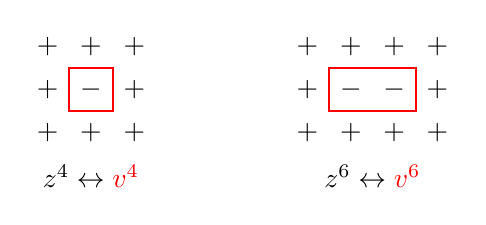
\begin{tikzpicture}[scale=0.55]
  \foreach \x/\y/\s in {0/0/+,1/0/+,2/0/+,0/1/+,1/1/-,2/1/+,0/2/+,1/2/+,2/2/+} \node at (\x,\y) {$\s$};
  \draw[red,thick] (0.5,0.5) rectangle (1.5,1.5);
  \node at (1,-1) {$z^4\leftrightarrow{\color{red}v^4}$};
  \begin{scope}[xshift=6cm]
  \foreach \x/\y/\s in {0/0/+,1/0/+,2/0/+,3/0/+,0/1/+,1/1/-,2/1/-,3/1/+,0/2/+,1/2/+,2/2/+,3/2/+} \node at (\x,\y) {$\s$};
  \draw[red,thick] (0.5,0.5) rectangle (2.5,1.5);
  \node at (1.5,-1) {$z^6\leftrightarrow{\color{red}v^6}$};
  \end{scope}
\end{tikzpicture}
\diagramcaption{One- and two-spin flips in the low-temperature expansion and the corresponding
closed polygons on the dual lattice in the high-temperature expansion.}
\end{diagram}

$T_c$ occurs at the point where the high-$T$ and low-$T$ expansions coincide, i.e.\ at $z = v$. Now
\begin{equation}
  v = \tanh K = \frac{e^K-e^{-K}}{e^K+e^{-K}} = \frac{1-e^{-2K}}{1+e^{-2K}} = \frac{1-z}{1+z},
  \qquad\text{inverse:}\quad z = \frac{1-v}{1+v}.
\end{equation}
So $z = v$ is the equation
\begin{equation}
  z = \frac{1-z}{1+z},\qquad\text{i.e.}\quad z+z^2 = 1-z;\qquad z^2+2z-1 = 0 .
\end{equation}
Solutions: $z = (1/2)\left[-2\pm 2\sqrt2\right]$, i.e.\ $z = -1\pm\sqrt2$. The solution with a $-$
sign gives $z<0$, unphysical, so the unique physical solution is
\begin{equation}
  z = z_c = -1+\sqrt2 ;
\end{equation}
now $z = e^{-2K}$, so $e^{-2K_c} = \sqrt2-1$, so $-2K_c = \ln(\sqrt2-1)$, i.e.\
$K_c = -(1/2)\ln(\sqrt2-1) = +(1/2)\ln\left(1/(\sqrt2-1)\right)$
\begin{equation}
  \Rightarrow\quad K_c = \frac{1}{2}\ln(\sqrt2+1) = 0.4407 .
\end{equation}
Since $K = \beta J = J/(\kB T)$, this yields the result
\begin{equation}
  \kB T_c = \frac{J}{(1/2)\ln(\sqrt2+1)} = 2.269\,J .
\end{equation}
This derivation was obtained by Kramers and Wannier in 1941, before the Onsager calculation of the
free energy of the (zero-field) Ising model on the square lattice (which was published in 1944). Of
course, from a knowledge of the ($H = 0$) free energy, one can determine $T_c$, but the
Kramers--Wannier derivation of $T_c$ shows how one can sometimes determine some properties of a
stat.\ mech.\ system exactly even without knowing the free energy.

\section{The two-dimensional Ising model}
% Source: Lecture12.pdf, pages 1-7. Title on the source: "Lecture 12: Ising model in 2D".
\lecture{12}

In the previous lecture, we discussed the Kramers--Wannier derivation of $T_c$ in the Ising model on
the square lattice. Recall that since the square lattice is bipartite, we could, with no loss of
generality, assume $J>0$, hence $K = \beta J>0$. We used a low-temperature expansion in the variable
$z = e^{-2K}$ and a high-temperature expansion in the variable $v = \tanh K$, and showed a 1--1
correspondence between the terms in these expansions. The expansions extend from $T = \infty$ (i.e.\
$v = 0$) down and from $T = 0$ (i.e.\ $z = 0$) up, and meet at a unique point, which is the critical
point $T_c$. Equating the series for the partition function at $T = T_c$ (since the phase transition is
continuous), we set $z = v$. Now $v = (1-z)/(1+z)$, so this yields the equation
$z = (1-z)/(1+z)$, i.e.\ $z^2+2z-1 = 0$, with solutions $z = -1\pm\sqrt2$, of which only
$-1+\sqrt2$ is physical, since $-1-\sqrt2<0$, but $z = e^{-2K}$ is non-negative. So the critical point
is at $z = z_c = -1+\sqrt2$. Solving for $K_c$: $z_c = e^{-2K_c}$, $e^{-2K_c} = \sqrt2-1$,
$-2K_c = \ln(\sqrt2-1)$, so
\begin{equation}
  K_c = -\frac{1}{2}\ln(\sqrt2-1) = +\frac{1}{2}\ln\left(\frac{1}{\sqrt2-1}\right) = \frac{1}{2}\ln(\sqrt2+1) = 0.4407 .
\end{equation}
Note that we can equivalently obtain this result by using
$\operatorname{arctanh}x = (1/2)\ln[(1+x)/(1-x)]$:
with $v = v_c = \tanh K_c = \sqrt2-1$,
\begin{align}
  K_c &= \operatorname{arctanh}v_c = \frac{1}{2}\ln\left(\frac{1+v_c}{1-v_c}\right)
       = \frac{1}{2}\ln\left(\frac{1+(\sqrt2-1)}{1-(\sqrt2-1)}\right)\nonumber\\
      &= \frac{1}{2}\ln\left(\frac{\sqrt2}{2-\sqrt2}\right) = \frac{1}{2}\ln\left(\frac{1}{\sqrt2-1}\right) = \frac{1}{2}\ln(\sqrt2+1).
\end{align}
Then, with $K = J/(\kB T)$, solving for $T_c$,
\begin{equation}
  \kB T_c = \frac{J}{K_c} = \frac{J}{\frac{1}{2}\ln(\sqrt2+1)} = 2.269\,J .
\end{equation}
As we discussed earlier, this is lower than the MFT estimate, $K_{c,\text{MFT}} = 1/\Delta = 1/4$
here, i.e.\ $\kB T_{\text{MFT}} = J/K_{c,\text{MFT}} = 4J$. We saw the Peierls Theorem with plausible
estimates for the path branching parameter $c$ yields a value of $T_c$ comparable to the exact value:
$\kB T_c\simeq 2J/\ln c$; $2\le c\le 3$, and with $c = 2.5$, $\kB T_c = 2J/\ln(2.5) = 2.2J$.

\subsection{The 2D Ising model and its exact solution}
\subsubsection*{The Ising model in two dimensions}

We now proceed to discuss some relevant results for the Ising model on 2D lattices. We focus on the
square lattice for definiteness; the critical behavior is the same for the model with ferromagnetic
coupling $J>0$ on all 2D lattices. This is easy to understand: as $T\nearrow T_c$ or $T\searrow T_c$,
the correlation length $\xi\to\infty$, and hence short-distance details of lattice structure become
irrelevant; e.g.\ it does not matter for the critical behavior whether the lattice is sq, tri, hc, or
some other regular lattice. This property will also be evident in the context of the renormalization
group, RG. On a bipartite lattice such as the sq and hc lattices, because of the isomorphism relating
the FM ($J>0$) and AFM ($J<0$) signs of $J$, with the corresponding mapping of uniform
$\leftrightarrow$ staggered magnetization, it follows that the critical behavior of the model with
$J<0$ is also independent of the lattice type.

However, it is not, in general, true that the FM and AFM versions of the model have the same critical
behavior on a non-bipartite lattice, since the AFM case may entail frustration. An example is the
Ising AFM on the triangular lattice, where the frustration removes the finite-temperature phase
transition.

\paragraph{Some helpful relations.}

Besides $v = (1-z)/(1+z)$, $z = (1-v)/(1+v)$, also:
\begin{align}
  \sinh K &= \frac{v}{\sqrt{1-v^2}} = \frac{1-z}{2\sqrt z}, &
  \sinh(2K) &= 2\sinh K\cosh K = \frac{2v}{1-v^2} = \frac{1-z^2}{2z},\\
  \cosh K &= \frac{1}{\sqrt{1-v^2}} = \frac{1+z}{2\sqrt z}, &
  \cosh(2K) &= \cosh^2K+\sinh^2K = \frac{1+v^2}{1-v^2} = \frac{1+z^2}{2z}.
\end{align}
N.B.: $\sinh 2K\to 1$ as $K\to K_c$, which can be seen with either expression as a function of $z$ or
$v$; e.g., with $z_c = \sqrt2-1$,
\begin{equation}
  \sinh 2K_c = \frac{(1+z_c)(1-z_c)}{2z_c} = \frac{\sqrt2(2-\sqrt2)}{2(\sqrt2-1)} = 1 .
\end{equation}
The quantity $\tilde k_>\equiv\sinh^22K$ will appear in correlation functions at $T>T_c$ and
$\tilde k_<\equiv1/\tilde k_> = 1/(\sinh^22K)$ in correlation functions at $T<T_c$. These
are equal and equal to 1 at $T_c$: $\tilde k_< = \tilde k_> = 1$ at $T_c$.

The quantity
\begin{equation}
  \kappa\equiv\frac{2\sinh 2K}{\cosh^22K}
\end{equation}
occurs in the specific heat. With the identity $\cosh^2x-\sinh^2x = 1$, one has
$\cosh^22K_c = 1+\sinh^22K_c = 2$, so $\kappa_c = 2\cdot 1/2 = 1$. As $K\to 0$ and
$K\to\pm\infty$, $\kappa\to 0$, so $\kappa$ reaches its maximal value of 1 at $K_c$.

\begin{diagram}
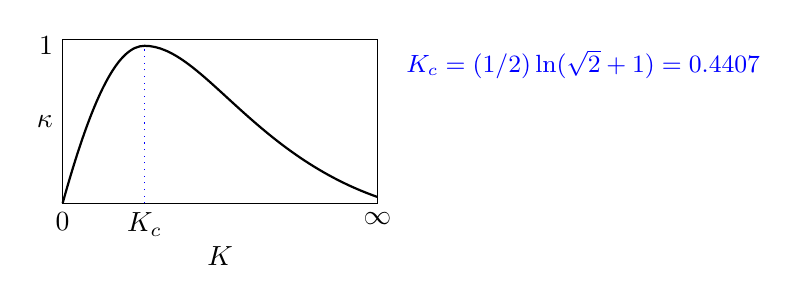
\begin{tikzpicture}[scale=0.8]
  \draw (0,0) rectangle (5,2.6);
  \draw[thick] (0,0) .. controls (0.5,1.8) and (0.9,2.5) .. (1.3,2.5) .. controls (2.2,2.5) and (3,0.8) .. (5,0.1);
  \draw[dotted,blue] (1.3,0) -- (1.3,2.5);
  \node[left] at (0,1.3) {$\kappa$};
  \node[below] at (0,0) {$0$}; \node[below] at (1.3,0) {$K_c$}; \node[below] at (5,0) {$\infty$};
  \node[below=12pt] at (2.5,0) {$K$};
  \node[left] at (0,2.5) {$1$};
  \node[blue,anchor=west,font=\small] at (5.3,2.2) {$K_c = (1/2)\ln(\sqrt2+1) = 0.4407$};
\end{tikzpicture}
\diagramcaption{The elliptic modulus $\kappa$ as a function of $K$.}
\end{diagram}

\subsubsection*{Exact results and their history}

The 2D Ising model was important in the historical development of stat.\ mech.\ and the theory of
critical phenomena because one could, at least for zero external magnetic field, $H = 0$, calculate
exact closed-form expressions for some (not all) thermodynamic quantities, in particular the Gibbs
free energy $G(T,H=0)$. This was calculated in 1944 by L.~Onsager. From this one can calculate the
internal energy $U(T,H=0)$ and the specific heat capacity $C_H(T,H=0)$ [L.~Onsager, Phys.\ Rev.\
\textbf{65}, 117 (1944)]. One finds that $C$ has a logarithmic divergence at $T_c$ (so
$\alpha = \alpha' = 0$). The spontaneous magnetization $M_{sp}$ was calculated by C.N.~Yang in 1952
[C.N.~Yang, Phys.\ Rev.\ \textbf{85}, 808 (1952)], yielding the critical exponent $\beta = 1/8$.
These values of critical exponents were of great interest because they differed from the predictions
of LG and MFT, which were that $C$ has a discontinuity at $T_c$ and that the critical exponent for the
magnetization is $\beta_{\text{MFT}} = 1/2$.

These calculations were initially for the square lattice and were later extended to other 2D lattices,
which gave the same values for the exponents, thereby providing analytical support for universality of
critical behavior, independent of lattice structure (in the absence of frustration). This was also very
important, since experiments on magnetic phenomena in different Ising-like (uniaxial) materials had
observed this universality (as had experiments on critical phenomena in liquid--gas systems; recall the
plot from Guggenheim showing the same $\beta\sim 0.35$ for the critical point in various gases). No
closed-form solutions have ever been obtained for the initial magnetic susceptibility
$\chi = \left.\partial M/\partial H\right|_{H=0}$ or for any of these quantities in a nonzero physical
external magnetic field $H$. However, later, a procedure was worked out for calculating
$\ev{\sigma_{\mathbf 0}\sigma_{\mathbf r}} = \ev{\sigma_{(0,0)}\sigma_{(i,j)}}$ by Montroll, Potts, and
Ward, and this was used to study the asymptotic behavior of the spin--spin correlation function to
infer the critical exponents $\nu$ and $\nu'$ describing the divergence in $\xi$ as $T\to T_c$ (recall
$\ev{\sigma_{\mathbf 0}\sigma_{\mathbf r}}_{\text{conn.}}\sim e^{-r/\xi}$ as $|\mathbf r| = r\to\infty$).
It was found that $\nu = \nu' = 1$. A similar study of the spin--spin correlation function at $T_c$
yielded $\eta = 1/4$ (recall $\ev{\sigma_{\mathbf 0}\sigma_{\mathbf r}}\sim 1/r^{d-2+\eta}$ at
$T = T_c$).

Although most experimental measurements of critical phenomena, such as liquid--gas systems (which are in
the Ising universality class) and magnetic systems, are 3D rather than 2D, these exact results for the
critical exponents of the 2D Ising model were valuable as a demonstration of non-MFT,
non-Landau--Ginzburg critical behavior.

\subsection{Free energy, internal energy and specific heat}
\subsubsection*{The free energy}

The reduced dimensionless free energy $f = f(T,H=0)$, where $G(T,H) = -\kB Tf(T,H)$, can be calculated
by a transfer matrix method similar to, but more complicated than, our use of this method in the 1D
model. The result for $f$ (for the square lattice) is
\begin{equation}
  f = \ln 2 + \frac{1}{2}\int_{-\pi}^{\pi}\frac{\dd\theta_1}{2\pi}\int_{-\pi}^{\pi}\frac{\dd\theta_2}{2\pi}
      \ln\left[L(\theta_1,\theta_2)\right],
\end{equation}
where $L = L(\theta_1,\theta_2)$ is
\begin{equation}
  L = \cosh^2(2K) - \sinh(2K)\cdot\mathcal{P},\qquad\text{with}\quad \mathcal{P} = \cos\theta_1+\cos\theta_2 .
\end{equation}
Over the range of integration, $\mathcal P$ varies from $-2$ to $+2$. The free energy $f$ has a
non-analyticity where $L = 0$. Now $\cosh^22K_c = 2$ and
$\sinh 2K_c = \begin{cases}1 & \text{for FM}\\ -1 & \text{for AFM}\end{cases}$, so one sees that this
non-analyticity occurs at $K = \pm K_c$:
\begin{align*}
  \text{FM case } J>0:&\quad L = 2 - 1\cdot\mathcal P = 0\quad\text{if } \mathcal P = 2,\\
  \text{AFM case } J<0:&\quad L = 2 - (-1)\cdot\mathcal P = 0\quad\text{if } \mathcal P = -2.
\end{align*}
As $T\to\infty$, $K\to 0$, $L\to 1$, $\ln L\to 0$, so $f\to\ln 2$. This reflects the fact that when
$\beta = 0$, the spin--spin interaction has no effect, so $Z = 2^N$,
$f = \lim_{N\to\infty}(1/N)\ln Z = \ln 2$; spins are completely random. For the other limit, without
loss of generality, assume $J>0$, so $K>0$, the FM case. As $T\to 0$, the spins approach a completely
ordered state (all $+$ or all $-$), so in $Z = \sum_{\{\sigma_i\}}e^{K\sum_{e_{ij}}\sigma_i\sigma_j}$, the
argument of the exponential $\to K\cdot e(\Lambda) = K\cdot(\Delta/2)n(\Lambda) = K(\Delta_{sq}/2)N = 2KN$
(with $\Delta_{sq} = 4$), so
\begin{equation}
  Z\to 2e^{2KN},\qquad \ln Z = \ln 2 + 2KN,\qquad f = \lim_{N\to\infty}\frac{1}{N}\ln Z\to 2K .
\end{equation}
We see how the exact result agrees with this as $T\to 0$:
$\cosh^2(2K) = \left((e^{2K}+e^{-2K})/2\right)^2\to e^{4K}/4$, which dominates over
$\sinh 2K\to e^{2K}/2$, so the $\theta$-independent first term in $L$ dominates over the
$\theta$-dependent term and
\begin{equation}
  f\to\ln 2 + \frac{1}{2}\int_{-\pi}^{\pi}\frac{\dd^2\theta}{(2\pi)^2}\ln\left(\frac{e^{4K}}{4}\right)
  = \ln 2 + \frac{1}{2}(4K - 2\ln 2) = 2K,
\end{equation}
since $\int_{-\pi}^{\pi}\dd^2\theta/(2\pi)^2 = 1$.

It is also useful to express $f$ in terms of $z$ and $v$. Using $\cosh(2K) = (1+z^2)/(2z)$ and
$\sinh(2K) = (1-z^2)/(2z)$, with $\mathcal P = \cos\theta_1+\cos\theta_2$,
\begin{align}
  f &= \ln 2 + \frac{1}{2}\int_{-\pi}^{\pi}\frac{\dd^2\theta}{(2\pi)^2}\ln\left[\cosh^2(2K)-\sinh(2K)\mathcal P\right]\nonumber\\
    &= \ln 2 + \frac{1}{2}\int_{-\pi}^{\pi}\frac{\dd^2\theta}{(2\pi)^2}\ln\left[\frac{(1+z^2)^2}{(2z)^2}-\frac{(1-z^2)}{2z}\mathcal P\right]\nonumber\\
    &= \underbrace{\ln 2 - \ln(2z)}_{\ln 2-\ln 2-\ln(e^{-2K}) = 2K}
     + \frac{1}{2}\int_{-\pi}^{\pi}\frac{\dd^2\theta}{(2\pi)^2}\ln\left[(1+z^2)^2 - 2z(1-z^2)\mathcal P\right].
\end{align}
Although one cannot do both of the integrations, it is possible to do one. This gives $f$ in terms of a
single integral (HW):
\begin{equation}
  f = \ln\left(2\cosh(2K)\right) + \frac{1}{2}\int_0^\pi\frac{\dd\phi}{\pi}
      \ln\left[\frac{1+\sqrt{1-\kappa^2\sin^2\phi}}{2}\right],
\end{equation}
where, as above, $\kappa = 2\sinh(2K)/\cosh^2(2K)$ ($\kappa\to-\kappa$ as $J\to-J$, FM vs.\ AFM sign). This again exhibits a non-analyticity at
$\kappa = 1$, where the argument of the square root can vanish.

\subsubsection*{Internal energy and specific heat}

Then, $\bar U = -\partial f/\partial \beta = -J\partial f/\partial K$ $\Rightarrow$
\begin{equation}
  \bar U = -J\coth(2K)\left[1 + \frac{2}{\pi}\left(2\tanh^2(2K)-1\right)K(\kappa)\right],
\end{equation}
where
\begin{equation}
  K(\kappa) = \int_0^{\pi/2}\frac{\dd\omega}{\sqrt{1-\kappa^2\sin^2\omega}}
\end{equation}
is the complete elliptic integral of the first kind and $\kappa$ is the elliptic modulus. Here we follow
standard mathematical notation; do not confuse this $K(\kappa)$ with $K = \beta J$. Note that $K(\kappa)$
only depends on $\kappa^2$.

An important property of $K(\kappa)$ is that $K(\kappa)$ diverges logarithmically as $\kappa^2\to 1$.
Since $K(\kappa)$ only depends on $\kappa^2$, the FM and AFM signs of $J$ are equivalent. The prefactor
$2\tanh^2(2K)-1\to(2\cdot1/2-1)\to 0$ as $K\to K_c$, so that $\bar U$ is finite
($\lim_{x\to 0}x\ln x = 0$) but is non-analytic at $K_c$. To see the log divergence in $K(\kappa)$ as
$|\kappa|\to 1$, note that if $\kappa = \pm 1$, then
\begin{equation}
  \int\frac{\dd\omega}{\sqrt{1-\sin^2\omega}} = \int\frac{\dd\omega}{\cos\omega}
  = \ln(\sec\omega+\tan\omega) = \ln\left(\frac{1+\sin\omega}{\cos\omega}\right),
\end{equation}
and the evaluation at $\omega = \pi/2$ then gives $\ln(1/0) = \ln\infty$. As $\kappa\to 0$,
$K(\kappa)$ has the Taylor series expansion
$K(\kappa) = (\pi/2)\left[1+\kappa^2/4+\Order(\kappa^4)\right]$, so, in
\begin{equation}
  \bar U = -\frac{J}{\tanh(2K)}\left[1+\frac{2}{\pi}\left(2\tanh^2(2K)-1\right)K(\kappa)\right],
\end{equation}
as $T\to 0$, $K\to\infty$, $\kappa\to 0$, so $K(\kappa)\to\pi/2$ and
\begin{equation}
  \bar U\to\frac{-J}{\tanh(2K)}\left[1+(2\tanh^2(2K)-1)\right] = -2J\tanh(2K)\to -2J .
\end{equation}
In general, on a lattice $\Lambda$ with coordination number (vertex degree) $\Delta$, as $T\to 0$, all
spins are aligned and $\bar U\to-(\Delta/2)J$; here, with $\Delta = 4$, we see that the result agrees
with this limit.

Then calculating
\begin{equation}
  \bar C_H = \pder{\bar U}{T} = \pder{K}{T}\cdot\pder{\bar U}{K} = -\frac{\kB K^2}{J}\pder{\bar U}{K}
  = \kB K^2\frac{\partial^2f}{\partial K^2}
\end{equation}
and then taking the limit as $K\to K_c$, one finds
\begin{equation}
  \bar C_H\propto-\ln(|K-K_c|),\qquad\text{i.e.}\quad \bar C_H\propto-\ln(|T-T_c|)\quad\text{as } T\to T_c .
\end{equation}
This is not an algebraic singularity,
$\begin{cases}|T-T_c|^{-\alpha} & \text{for } T\searrow T_c\\ |T-T_c|^{-\alpha'} & \text{for } T\nearrow T_c\end{cases}$,
but if one fits it with a power law it corresponds to $\alpha = \alpha' = 0$.

\subsection{Correlation functions, magnetization and critical exponents}

The spin--spin correlation functions are polynomials in complete elliptic integrals $K(\tilde k)$ and
$E(\tilde k)$, where
\begin{equation}
  \tilde k = \begin{cases}\tilde k_> = \sinh^2(2K) & \text{for } T>T_c\\
                          \tilde k_< = [\sinh^2(2K)]^{-1} & \text{for } T<T_c,\end{cases}
\end{equation}
with
\begin{equation}
  K(\tilde k) = \int_0^{\pi/2}\frac{\dd\omega}{\sqrt{1-\tilde k^2\sin^2\omega}}
  \qquad\text{and}\qquad
  E(\tilde k) = \int_0^{\pi/2}\dd\omega\,\sqrt{1-\tilde k^2\sin^2\omega},
\end{equation}
the complete elliptic integral of the second kind. For small $\tilde k$, one has
$E(\tilde k) = (\pi/2)[1-\tilde k^2/4+\Order(\tilde k^4)]$. For $\tilde k = 1$,
$E(\tilde k) = \int_0^{\pi/2}\cos\omega\,\dd\omega = \left.\sin\omega\right|_0^{\pi/2} = 1$.

\begin{diagram}
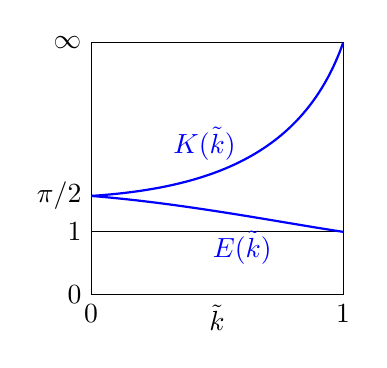
\begin{tikzpicture}[scale=0.8]
  \draw (0,0) rectangle (4,4);
  \draw (0,1.0) -- (4,1.0);
  \draw[thick,blue] (0,1.57) .. controls (2,1.7) and (3.4,2.3) .. (4,4);
  \draw[thick,blue] (0,1.57) .. controls (1.5,1.45) and (3,1.15) .. (4,1.0);
  \node[left] at (0,1.57) {$\pi/2$}; \node[left] at (0,1.0) {$1$}; \node[left] at (0,0) {$0$};
  \node[left] at (0,4) {$\infty$};
  \node[below] at (0,0) {$0$}; \node[below] at (4,0) {$1$}; \node[below] at (2,0) {$\tilde k$};
  \node[blue] at (1.8,2.4) {$K(\tilde k)$};
  \node[blue] at (2.4,0.75) {$E(\tilde k)$};
\end{tikzpicture}
\diagramcaption{The complete elliptic integrals $K(\tilde k)$ and $E(\tilde k)$.}
\end{diagram}

The nearest-neighbor correlation function is
\begin{equation}
  \ev{\sigma_{00}\sigma_{10}} = \ev{\sigma_{00}\sigma_{01}} =
  \begin{cases}
    \sqrt{1+\tilde k_>^{-1}}\left[\dfrac{1}{2} + (\tilde k_>-1)\dfrac{K(\tilde k_>)}{\pi}\right] & \text{for } T>T_c\\[10pt]
    \sqrt{1+\tilde k_<}\left[\dfrac{1}{2} - (\tilde k_<-1)\dfrac{K(\tilde k_<)}{\pi}\right] & \text{for } T<T_c .
  \end{cases}
\end{equation}
These are both $=1/\sqrt2$ at $T = T_c$.

C.N.~Yang: the spontaneous magnetization is
\begin{equation}
  M_{sp} = (1-\tilde k_<^2)^{1/8}\ \Rightarrow\ \beta = \frac{1}{8} .
\end{equation}
Via the relation $\bar\chi = \sum_{\mathbf r}\ev{\sigma_{\mathbf 0}\sigma_{\mathbf r}}_{\text{conn.}}$,
calculate the asymptotic behavior of $\bar\chi$ $\Rightarrow\gamma = \gamma' = 7/4$:
\begin{equation}
  \bar\chi\sim\begin{cases}\dfrac{1}{|T-T_c|^{\gamma}} & T>T_c\\[8pt] \dfrac{1}{|T-T_c|^{\gamma'}} & T<T_c,\end{cases}
\end{equation}
and the critical decay at $T_c$:
\begin{equation}
  \ev{\sigma_{\mathbf 0}\sigma_{\mathbf r}}\sim\frac{1}{r^{d-2+\eta}} = \frac{1}{r^\eta},\qquad\text{where }\eta = \frac{1}{4} ;
\end{equation}
also $\delta = 15$, with $M\sim H^{1/\delta}\sgn(H)$ at $T_c$.

\subsubsection*{Summary of critical exponents in the 2D Ising model and comparison with Landau--Ginzburg and MFT}

\begin{center}
\renewcommand{\arraystretch}{1.25}
\begin{tabular}{lcc}
  & LG/MFT & 2D Ising\\ \hline
  $\alpha,\alpha'$ & 0 (disc.) & 0 (log div.)\\
  $\beta$ & $1/2$ & $1/8$\\
  $\gamma,\gamma'$ & 1 & $7/4$\\
  $\nu,\nu'$ & $1/2$ & 1\\
  $\eta$ & 0 & $1/4$\\
  $\delta$ & 3 & 15
\end{tabular}
\end{center}
Later, we will show that these critical exponents depend on only two fundamental exponents, $y_T$, the
thermal exponent, and $y_h$, the magnetic exponent.

\section{Other spin models}
% Source: Lecture13.pdf, pages 1-8 (pages 9-10 are blank).
% Title on the source: "Lecture 13 - Other spin models".
\lecture{13}
\subsection{Generalized Ising models}
\subsubsection*{The anisotropic Ising model}

The spontaneous magnetization in the square-lattice Ising model (C.N.~Yang) is
\begin{equation}
  \bar M_{sp} = (1-\tilde k_<^2)^{1/8},\qquad\text{where}\quad \tilde k_< = \frac{1}{\tilde k_>} = \frac{1}{\sinh^2(2K)}.
\end{equation}
The free energy (and $\bar U$, $\bar C$, $\bar M_{sp}$) have also been calculated for other 2D lattices
and for the generalized case in which the spin--spin couplings are different in different lattice
directions, e.g.\ on the square lattice, for the ``anisotropic'' Ising model with
\begin{equation}
  \Ham = -\sum_{\mathbf r}\left(J_1\sigma_{\mathbf r}\sigma_{\mathbf r+\hat{\mathbf e}_1}
         + J_2\sigma_{\mathbf r}\sigma_{\mathbf r+\hat{\mathbf e}_2}\right),
\end{equation}
where $\hat{\mathbf e}_1 = \hat{\mathbf x}$ is a unit vector in the $x$ direction and
$\hat{\mathbf e}_2 = \hat{\mathbf y}$ is a unit vector in the $y$ direction. Define $K_1 = \beta J_1$
and $K_2 = \beta J_2$, $z_1 = e^{-2K_1}$, $z_2 = e^{-2K_2}$, $v_1 = \tanh K_1$, $v_2 = \tanh K_2$. Then
\begin{gather}
  f = \ln 2 + \frac{1}{2}\int_{-\pi}^{\pi}\frac{\dd^2\theta}{(2\pi)^2}\ln L,\nonumber\\
  L = \cosh(2K_1)\cosh(2K_2) - \sinh(2K_1)\cos\theta_1 - \sinh(2K_2)\cos\theta_2 .
\end{gather}
The critical temperature is defined by the condition
\begin{equation}
  \sinh(2K_1)\sinh(2K_2) = 1,\qquad\text{i.e.}\quad
  \sinh\left(\frac{2J_1}{\kB T_c}\right)\sinh\left(\frac{2J_2}{\kB T_c}\right) = 1 .
\end{equation}
This is the generalization of the condition $\sinh^2(2K) = 1$ in the isotropic ($J_1 = J_2$) case;
recall that for the isotropic case
\begin{equation}
  f = \ln 2 + \frac{1}{2}\int_{-\pi}^{\pi}\frac{\dd^2\theta}{(2\pi)^2}\ln\left[\cosh^2(2K)-\sinh(2K)(\cos\theta_1+\cos\theta_2)\right].
\end{equation}
For the FM case, the criticality condition gives a phase structure in the $K_1$--$K_2$ plane.

\begin{diagram}
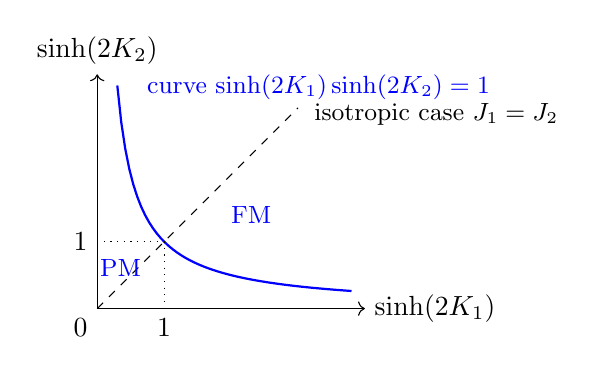
\begin{tikzpicture}[scale=0.85]
  \draw[->] (0,0) -- (4,0) node[right] {$\sinh(2K_1)$};
  \draw[->] (0,0) -- (0,3.5) node[above] {$\sinh(2K_2)$};
  \draw[thick,blue,domain=0.3:3.8,samples=60] plot (\x,{1/\x});
  \draw[dashed] (0,0) -- (3,3);
  \draw[dotted] (0,1) -- (1,1) -- (1,0);
  \node[below] at (1,0) {$1$}; \node[left] at (0,1) {$1$}; \node[below left] at (0,0) {$0$};
  \node[blue,font=\small] at (0.35,0.6) {PM};
  \node[blue,font=\small] at (2.3,1.4) {FM};
  \node[blue,anchor=west,font=\small] at (0.6,3.3) {curve $\sinh(2K_1)\sinh(2K_2) = 1$};
  \node[anchor=west,font=\small] at (3.1,2.9) {isotropic case $J_1 = J_2$};
\end{tikzpicture}
\diagramcaption{Phase structure of the anisotropic square-lattice Ising ferromagnet.}
\end{diagram}

Thus one can get FM LRO with a smaller $J_1$ and larger $J_2$ or vice versa, as well as the isotropic
case, $J_1 = J_2$. Here $\tilde k\to\tilde k_> = \sinh(2K_1)\sinh(2K_2)$, $\tilde k_< = (\tilde k_>)^{-1}$,
and $\bar M_{sp} = (1-\tilde k_<^2)^{1/8}$ as before. The critical behavior is the same as in the
isotropic case (provided that there is no frustration, e.g.\ for the FM case $J_i>0$ on all 2D lattices
and the AFM case on bipartite lattices).

There is a generalization of the FM and AFM ordering. E.g.\ on the square lattice as $T\to 0$, the LRO
is all $+$ or all $-$ for the FM, and the two checkerboard (N\'eel) patterns for the AFM. Now, again on
the square lattice, in addition to the FM case $\{J_1>0,J_2>0\}$ and the AFM case $\{J_1<0,J_2<0\}$,
there are the two mixed cases $\{J_1>0,J_2<0\}$ and $\{J_1<0,J_2>0\}$. These lead to a low-temperature
ordering as $T\to 0$ in which rows (for $J_1>0$, $J_2<0$) or columns (for $J_1<0$, $J_2>0$) alternate
in sign:
\begin{equation*}
  J_1>0,\ J_2<0:\quad
  \begin{array}{cccccc}
    - & - & - & - & - & -\\ + & + & + & + & + & +\\ - & - & - & - & - & -\\ + & + & + & + & + & +
  \end{array}
  \qquad\qquad
  J_1<0,\ J_2>0:\quad
  \begin{array}{cccccc}
    + & - & + & - & + & -\\ + & - & + & - & + & -\\ + & - & + & - & + & -\\ + & - & + & - & + & -
  \end{array}
\end{equation*}

\subsubsection*{Universality and additional couplings}

The fact that the critical behavior is the same for all of these cases (when there is no frustration)
is an example of the property that the critical behavior depends on the symmetry group of the
zero-field Hamiltonian (and the related space of the order parameter) and the dimensionality of the
lattice, but not on details of the lattice structure (2D: sq, tri, hc, \ldots; 3D: sc, bcc, fcc, hcp,
\ldots) or the spin--spin couplings (provided they are not $=0$ or $\infty$). Recall that $\Ham$ is
invariant under $\mathbb{Z}_2$ transformations (with group elements $\{1,-1\}$, where the $-1$ element
means $\sigma_i\to-\sigma_i\ \forall\,i$), independent of whether $J_1 = J_2$ or $J_1\ne J_2$, given zero
external field.

Thus, for example, this universality of the critical behavior means that the critical behavior is the
same if we add additional spin--spin couplings that respect the $\mathbb{Z}_2$ symmetry. For example,
in addition to the nearest-neighbor couplings, we could add next-nearest-neighbor couplings such as
\begin{align}
  \Ham = &-J_1\sum_{\mathbf r}\sigma_{\mathbf r}\sigma_{\mathbf r+\hat{\mathbf e}_1}
          - J_2\sum_{\mathbf r}\sigma_{\mathbf r}\sigma_{\mathbf r+\hat{\mathbf e}_2}\nonumber\\
         &- J_{\text{diag.}}\sum_{\mathbf r}\sigma_{\mathbf r}\sigma_{\mathbf r+\hat{\mathbf e}_1+\hat{\mathbf e}_2}
          &&\text{(e.g.\ }\sigma_{(0,0)}\sigma_{(1,1)})\nonumber\\
         &- J_{1,nnn}\sum_{\mathbf r}\sigma_{\mathbf r}\sigma_{\mathbf r+2\hat{\mathbf e}_1}
          &&\text{(e.g.\ }\sigma_{(0,0)}\sigma_{(2,0)})\nonumber\\
         &- J_{2,nnn}\sum_{\mathbf r}\sigma_{\mathbf r}\sigma_{\mathbf r+2\hat{\mathbf e}_2} + \cdots
          &&\text{(e.g.\ }\sigma_{(0,0)}\sigma_{(0,2)}).
\end{align}
These are all invariant under the $\mathbb{Z}_2$ symmetry of the $H = 0$ theory. Although one cannot
solve for $f(T,H=0)$ when these additional terms are present, they do not change the critical behavior
(assuming that they do not produce frustration). The approximation of keeping only nn spin--spin
couplings is usually a good one, although there are some materials where nnn spin--spin couplings are
non-negligible.

Note that in contrast, if one added an interaction term to $\Ham$ that violates the $\mathbb{Z}_2$
symmetry of the zero-field theory, such as a 3-spin coupling
$-J_{3sa}\sum_{\mathbf r}\sigma_{\mathbf r}\sigma_{\mathbf r+\hat{\mathbf e}_1}\sigma_{\mathbf r+\hat{\mathbf e}_2}$
(an ``L'' of three sites) or
$-J_{3sb}\sum_{\mathbf r}\sigma_{\mathbf r}\sigma_{\mathbf r+\hat{\mathbf e}_1}\sigma_{\mathbf r+2\hat{\mathbf e}_1}$
(three sites in a row), this \emph{does} change the critical behavior.

\subsubsection*{The spin-\texorpdfstring{$s$}{s} Ising model}

Another generalization of the Ising model is to have the spin variable $s_i$ take on more than 2 values,
in a way that retains the $\mathbb{Z}_2$ invariance, namely $s_i\in\{-s,-s+1,\ldots,s-1,s\}$. This is
called the ``spin-$s$ Ising model'' and is a natural classical model reflecting the property that a
quantum spin is a representation $s$ of $SU(2)$, with states
$\{|s,m_s\rangle\} = \{|s,-s\rangle,|s,-s+1\rangle,\ldots,|s,s-1\rangle,|s,s\rangle\}$, e.g.\
$s = 1/2$: $\{|1/2,-1/2\rangle,|1/2,1/2\rangle\}$; $s = 1$:
$\{|1,-1\rangle,|1,0\rangle,|1,1\rangle\}$, etc. With appropriate rescalings the spin-$1/2$ Ising
model then has $\sigma_i\in\{-1,1\}$, the spin-1 Ising model has $s_i\in\{-1,0,1\}$, etc., with
\begin{equation}
  \Ham = -J\sum_{e_{ij}}s_is_j,\qquad Z = \sum_{\{s_i\}}e^{-\beta\Ham}.
\end{equation}
Because this model has the same $\mathbb{Z}_2$ invariance, it has the same critical behavior. But it is
less studied because one has not been able to obtain an exact closed-form solution for $f$, $U$, $M$,
etc.\ even in the case of zero external magnetic field.

\subsection{The \texorpdfstring{$q$}{q}-state Potts model}

Another type of discrete spin model is the $q$-state Potts model. We have shown the equivalence of the
$q = 2$ Potts model and the (spin-$1/2$) Ising model. With zero-field
$\Ham = -J_P\sum_{e_{ij}}\delta_{\sigma_i\sigma_j}$, the symmetry group of the $q$-state Potts model is
the group of permutations of $q$ objects, $S_q$, of order $q!$. An example illustrates this invariance:
say $q = 3$. Then in the interaction of two adjacent spins, there are $q^2 = 9$ possible values of the
pair $\sigma_i\sigma_j$: the pairs $11$, $22$, $33$ with $\delta_{\sigma_i\sigma_j} = 1$, and the pairs
$12$, $21$, $13$, $31$, $23$, $32$ with $\delta_{\sigma_i\sigma_j} = 0$. Now transform all the spins
globally by one of the $q!$ elements of the permutation group $S_q$. Denote this element of $S_q$ by
$g$; $g(\sigma_i) = \sigma_i'$. For the cases where $\sigma_i = \sigma_j$, $g(\sigma_i) = g(\sigma_j)$, so
$\delta_{\sigma_i\sigma_j} = \delta_{g(\sigma_i)g(\sigma_j)} = 1$. By the definition of a group $G$, every
$g$ in $G$ has an inverse, $g^{-1}$, such that $gg^{-1} = g^{-1}g = 1$. If $\sigma_i\ne\sigma_j$, then
$g(\sigma_i)\ne g(\sigma_j)$, since if $g(\sigma_i) = g(\sigma_j)$, then
$g^{-1}g(\sigma_i) = \sigma_i = g^{-1}g(\sigma_j) = \sigma_j$, contradicting the assumption that
$\sigma_i\ne\sigma_j$. Since $\sigma_i\ne\sigma_j\Rightarrow g(\sigma_i)\ne g(\sigma_j)$,
$\delta_{\sigma_i\sigma_j} = \delta_{g(\sigma_i)g(\sigma_j)} = 0$. This proves that the zero-field Potts
$\Ham$ is invariant under $S_q$. Note that $S_2\approx\mathbb{Z}_2$. An external magnetic field term
$-H\sum_i\delta_{\sigma_i,1}$ breaks the $S_q$ symmetry explicitly and a spontaneous magnetization
$\ev{\sigma_i}$ breaks the $S_q$ symmetry spontaneously.

Recall the cluster formula (here $G$ means graph):
\begin{equation}
  Z(G,q,v_P) = \sum_{G'\subseteq G}q^{k(G')}v_P^{e(G')},
\end{equation}
where $G'$ = spanning subgraph of $G$, $v_P = e^{K_P}-1$ appearing in the identity
$e^{K_P\delta_{\sigma_i\sigma_j}} = 1 + v_P\delta_{\sigma_i\sigma_j}$, and $k(G')$ = \# of connected
components in $G'$, $e(G')$ = \# edges (= bonds) in $G'$. This cluster formula allows one to formally
generalize $q$ from a positive integer $q = 2,3,\ldots$ to a non-negative real number while keeping
$Z(G,q,v_P)>0$ (``Gibbs measure'') for FM $J_P>0$.

The $q$-state Potts ferromagnet has a continuous phase transition in 2D for $0<q\le 4$ ($Z = 0$ for
$q = 0$, but one can define $\tilde Z\equiv\lim_{q\to 0}(q^{-1}Z)$ to deal with the $q = 0$ case).

One commonly restricts to the integer cases $q = 2,3,4$, which have Hamiltonian representations. In
addition to the $q = 2$ (Ising) case, these provide interesting examples of critical behavior in 2D. In
contrast to the $q = 2$ Ising case, for $q\ne 2$, no closed-form expression has ever been calculated for
$f(T,H=0)$ (and obviously also not for $f(T,H\ne 0)$), but the critical exponents have been determined,
and they are rational, just as was true for the $q = 2$ case. For example, for the $q = 3$ Potts
ferromagnet in 2D, these exponents are
\begin{align*}
  q = 3:&\quad \alpha = \alpha' = \frac{1}{3},\enspace \beta = \frac{1}{9},\enspace \gamma = \gamma' = \frac{13}{9},
          \quad \nu = \nu' = \frac{5}{6},\enspace \delta = 14,\enspace \eta = \frac{4}{15},\\
  \text{vs. } q = 2:&\quad \alpha = \alpha' = 0\ \text{(log div.)},\enspace \beta = \frac{1}{8},\quad
          \gamma = \gamma' = \frac{7}{4},\enspace \nu = \nu' = 1,\enspace \delta = 15,\enspace \eta = \frac{1}{4} .
\end{align*}
The $q = 1$ Potts model, defined in the usual way, is trivial, since $\delta_{\sigma_i\sigma_j} = 1\ \forall\,i,j$,
so
\begin{equation}
  Z(\Lambda,q=1,v_P) = e^{K_Pe(\Lambda)} = e^{K_P(\Delta/2)n(\Lambda)},\qquad
  f = \lim_{n\to\infty}n^{-1}\ln Z = K_P\frac{\Delta}{2} .
\end{equation}

\subsubsection*{Landau--Ginzburg theory with a cubic term}

An interesting point concerns the Landau--Ginzburg formalism applied to the Potts model for $q\ne 2$,
e.g.\ $q = 3$. Because there is no $\mathbb{Z}_2$ invariance, the LG form of the Helmholtz free energy
$A(T,M)$ contains a cubic term:
\begin{equation}
  A(T,M) = L_0 + L_1M + L_2M^2 + L_3M^3 + L_4M^4 .
\end{equation}
As before, the $L_0$ term does not affect the determination of the minima of $A$, and the $L_1M$ term is
absent since otherwise $\left.\partial A/\partial M\right|_{M=0}\ne 0$, so $M = 0$ could not be a minimum of $A$ even at
high $T$. So
\begin{equation}
  A(T,M) = L_2M^2 + L_3M^3 + L_4M^4 .
\end{equation}
This can lead to a first-order transition.

\begin{diagram}
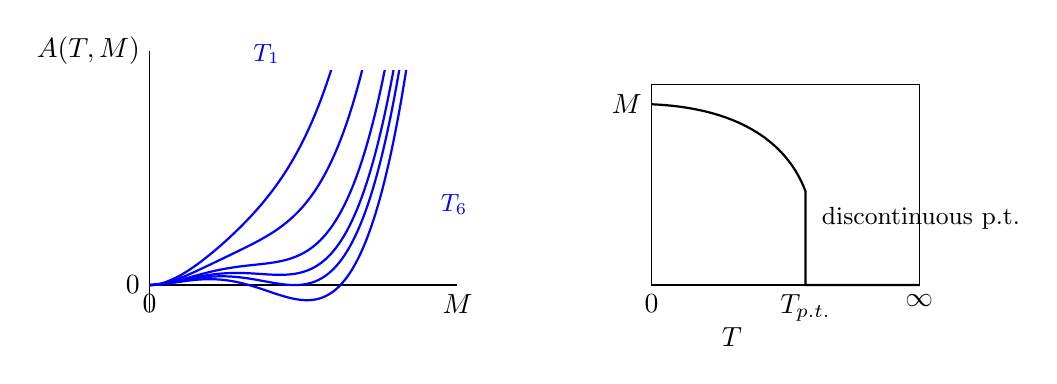
\begin{tikzpicture}[scale=0.85]
  \draw (0,-0.4) -- (0,3.5) node[left] {$A(T,M)$}; \draw (0,0) -- (4.6,0) node[below] {$M$};
  \begin{scope}
  \clip (0,-0.5) rectangle (4.5,3.2);
  \foreach \a in {1.6,1.25,1.0,0.9,0.833,0.75} {
    \draw[blue,thick,domain=0:3.4,samples=80,smooth] plot ({1.3*\x},{0.9*(\a*\x*\x - \x*\x*\x + 0.3*\x*\x*\x*\x)});
  }
  \end{scope}
  \node[blue,font=\small] at (1.75,3.45) {$T_1$};
  \node[blue,font=\small] at (4.55,1.2) {$T_6$};
  \node[left] at (0,0) {$0$}; \node[below] at (0,0) {$0$};
  \begin{scope}[xshift=7.5cm]
    \draw (0,0) rectangle (4,3);
    \draw[thick] (0,2.7) .. controls (1.2,2.65) and (2.0,2.2) .. (2.3,1.4) -- (2.3,0) -- (4,0);
    \node[below] at (0,0) {$0$}; \node[below] at (2.3,0) {$T_{p.t.}$}; \node[below] at (4,0) {$\infty$};
    \node[below=12pt] at (1.2,0) {$T$};
    \node[left] at (0,2.7) {$M$};
    \node[anchor=west,font=\small] at (2.4,1.0) {discontinuous p.t.};
  \end{scope}
\end{tikzpicture}
\diagramcaption{For $q\ne 2$: Landau--Ginzburg free energy with a cubic term, for
$T_1>T_2>\cdots>T_6$. As $T\searrow T_5$, the minimum of $A$ jumps discontinuously from the
$S_3$-symmetric value $M = 0$ to a nonzero value.}
\end{diagram}

It turns out that the phase transition between the $S_q$-symmetric high-temperature phase and the
low-temperature phase with spontaneous breaking of the $S_q$ symmetry and ferromagnetic LRO is
first-order for the $q$-state Potts model with $q\ne 2$ in $d = 3$, and in $d = 2$ for $q>4$, while for
$0\le q\le 4$, it is continuous. (The $q = 1$ case is trivial when defined by setting $q = 1$ before
taking the thermodynamic limit, but this does not commute with the opposite order of limits, i.e.\ the
thermodynamic limit first, with $q\in\mathbb{R}$, $q\ne 1$, and then letting $q\to 1$.)

\subsection{Continuous-spin models}
\subsubsection*{The Mermin--Wagner theorem}

Now proceed to continuous-spin models, e.g.\ $O(N)$ spin models with
\begin{equation}
  \Ham = -J\sum_{e_{ij}}\mathbf{S}_i\cdot\mathbf{S}_j - \mathbf{H}\cdot\sum_i\mathbf{S}_i,\qquad
  \mathbf{S}_i\in S^{N-1},\qquad
  Z = \int\left[\prod_i\dd\mathbf{S}_i\right]e^{-\beta\Ham},
\end{equation}
with $\mathbf{S}_i = (S_{1i},S_{2i},\ldots,S_{Ni})$, $|\mathbf{S}_i| = 1$, e.g.\ for $N = 2$,
$\mathbf{S}_i = (S_{1i},S_{2i}) = (\cos\theta_i,\sin\theta_i)$.

Recall a basic difference in the LG Helmholtz energy as a function of $M$ in the $\mathbb{Z}_2$ Ising
case (formally, $N = 1$ $O(N)$) and $O(N)$, $N\ge 2$. Illustrate this for $O(2)$:
$\mathbf{M} = \ev{\mathbf{S}} = \ev{(S_1,S_2)}$, with $M = |\mathbf{M}|$, $M_1 = \ev{S_1}$,
$M_2 = \ev{S_2}$.

\begin{diagram}
\begin{tikzpicture}[scale=0.75]
  \draw (-2,0) -- (2,0) node[right] {$M$}; \draw (0,-0.3) -- (0,2.4) node[above] {$A(T,M)$};
  \draw[thick,blue,domain=-1.7:1.7,samples=50] plot (\x,{0.6*\x*\x});
  \node[font=\small,anchor=west] at (1.2,2.0) {$T>T_c$};
  \begin{scope}[yshift=-4cm]
  \draw (-2,0) -- (2,0) node[right] {$M$}; \draw (0,-0.6) -- (0,2.4) node[above] {$A(T,M)$};
  \draw[thick,blue,domain=-1.9:1.9,samples=80] plot (\x,{-0.9*\x*\x+0.35*\x*\x*\x*\x});
  \node[font=\small,anchor=west] at (1.2,2.0) {$T<T_c$};
  \node[font=\small] at (0,-1.1) {2 discrete minima};
  \end{scope}
  \node[font=\small] at (0,-6.7) {Ising};
  \begin{scope}[xshift=7.5cm]
    \draw[thick,blue] (-1.8,2.2) .. controls (-1.2,0.2) and (-0.4,0) .. (0,0) .. controls (0.4,0) and (1.2,0.2) .. (1.8,2.2);
    \draw[blue] (0,2.2) ellipse (1.8 and 0.3);
    \draw (0,0) -- (0,2.9) node[above] {$A(T,M)$};
    \draw (0,0) -- (2.6,0.35) node[right] {$M_2$}; \draw (0,0) -- (-2.1,-0.7) node[left] {$M_1$};
    \node[font=\small,anchor=west] at (2.0,1.6) {$T>T_c$};
    \begin{scope}[yshift=-4cm]
      \draw[thick,blue] (-1.8,2.2) .. controls (-1.4,0.2) and (-1.0,-0.2) .. (-0.6,-0.2) .. controls (-0.3,-0.2) and (-0.2,0.25) .. (0,0.25)
            .. controls (0.2,0.25) and (0.3,-0.2) .. (0.6,-0.2) .. controls (1.0,-0.2) and (1.4,0.2) .. (1.8,2.2);
      \draw[blue] (0,2.2) ellipse (1.8 and 0.3);
      \draw[blue,dashed] (0,-0.2) ellipse (0.6 and 0.12);
      \draw (0,0.25) -- (0,2.9) node[above] {$A(T,M)$};
      \draw (0,0) -- (2.6,0.35) node[right] {$M_2$}; \draw (0,0) -- (-2.1,-0.7) node[left] {$M_1$};
      \node[font=\small,anchor=west] at (2.0,1.6) {$T<T_c$};
      \node[font=\small,align=center] at (0,-1.4) {surface of revolution: a circle,\\ forming a continuous ring of minima};
    \end{scope}
    \node[font=\small] at (0,-6.7) {$O(2)$};
  \end{scope}
\end{tikzpicture}
\diagramcaption{The Landau--Ginzburg free energy for the Ising and $O(2)$ models. (In the extension
to quantum field theory, the $m^2$ of a particle is the curvature of $V$,
$\partial^2V/\partial\phi^2|_{\min}$. N.B.: in the $O(2)$ case, this is 0 going around the ring of
degenerate minima.)}
\end{diagram}

This difference reflects the fact that the magnetization in the Ising model can only take on 2 values,
$M = \pm M_0$, but in the $O(2)$ model the vector spin can take on a continuous infinity of values,
$\mathbf{M} = (\cos\theta_0,\sin\theta_0)$ where $-\pi<\theta_0\le\pi$. To disorder incipient order in
the Ising model requires a discrete energy difference (flipping one spin in a sea of $+$ spins costs
$\Delta U = 2J\Delta = 8J$), whereas in contrast, to disorder an incipient ordered state in the $O(2)$
(in general, $O(N)$ with $N\ge 2$) model requires an arbitrarily small energy increment,
$\uparrow\uparrow\uparrow\uparrow\ \to\ \uparrow\uparrow\nearrow\nearrow$ etc. This is related to the
connected continuous $\infty$ of $\mathbf{M}$ values, all of which minimize $A(T,|\mathbf{M}|)$ at
$T<T_c$: the circular ring of minima for the $O(2)$ model shown in the graph.

This ease of disordering an incipient ordered state has the effect that a spin system at finite
temperature that is invariant under a continuous global symmetry group $G$ does not exhibit a phase
transition with spontaneous symmetry breaking (SSB) of this symmetry in $d = 2$ dimensions
(\emph{Mermin--Wagner Theorem}). This is connected with the Nambu--Goldstone Theorem, namely that
spontaneously breaking a continuous global symmetry leads to massless modes. In particle physics
(quantum field theory) these are massless elementary particles. In statistical mechanics, they are
modes disordering incipient order. In the illustrative $O(2)$ model, they can be seen as a consequence
of the continuous degeneracy of the minima of the energy: the circular ring of minima in the plot of
the free energy $A(T,M)$.

The case $T = 0$ is special, because here the minimization of the free energy reduces to the
minimization of the internal energy $U$, which is minimized for $M\ne 0$, i.e.\ nonzero spontaneous
magnetization (assuming no frustration).

This theorem does allow a system with a continuous symmetry group $G$ to have a finite-temperature phase
transition, as long as this does not spontaneously break the symmetry $G$, i.e.\ in a spin model, as
long as the spontaneous magnetization is zero.

\subsubsection*{The Kosterlitz--Thouless transition}

An example is the 2D $O(2)$ model with
\begin{equation}
  \Ham = -J\sum_{e_{ij}}\mathbf{S}_i\cdot\mathbf{S}_j,\qquad \mathbf{S}_i = (\cos\theta_i,\sin\theta_i).
\end{equation}
The 2D $O(2)$ model has a phase transition that involves dissociation of vortex pairs (``molecules'').
Recall that the vortices arise because the homotopy group $\pi_1(S^1)$ is nontrivial:
$\pi_1(S^1) = \mathbb{Z}$, where $\pi_1(G)$ is the set of continuous maps of $S^1\to G$. Now
$O(2)\sim U(1)\sim S^1$; spins ``live'' in $S^1$, the circle.

\begin{diagram}
\begin{tikzpicture}[scale=0.6,>=Stealth]
  \foreach \r in {0.7,1.3} \foreach \a in {0,45,...,315}
    \draw[->] ({\r*cos(\a)},{\r*sin(\a)}) -- ++({\a+90}:0.45);
  \node[font=\small,align=center] at (0,-2.6) {$n = 1$ element\\ of $\pi_1(S^1)$\\ (denote as v)};
  \begin{scope}[xshift=5cm]
  \foreach \r in {0.7,1.3} \foreach \a in {0,45,...,315}
    \draw[->] ({\r*cos(\a)},{\r*sin(\a)}) -- ++({-\a+90}:0.45);
  \node[font=\small,align=center] at (0,-2.6) {$n = -1$ element\\ of $\pi_1(S^1)$, opposite\\ vorticity (denote as $-$v)};
  \end{scope}
  \begin{scope}[xshift=10.5cm]
    \draw (0,0) ellipse (1.5 and 0.8); \node at (-0.6,0) {v}; \node at (0.6,0) {$-$v};
    \draw[->,blue] (1.8,0) -- (2.8,0);
    \node[blue,font=\small] at (2.3,1.1) {as $T\nearrow T_c$};
    \draw (3.6,0) circle (0.5); \node at (3.6,0) {v};
    \draw (5.0,0) circle (0.5); \node at (5.0,0) {$-$v};
    \node[font=\small,align=center] at (2.5,-2.6) {``topological\\ defect-driven p.t.''};
  \end{scope}
\end{tikzpicture}
\diagramcaption{Vortex configurations. At low $T$, the vortices are bound in vortex--antivortex pairs;
as $T\nearrow T_c$ the pairs dissociate.}
\end{diagram}

There is no magnetization in the low-temperature phase, and this phase transition does \emph{not} break
the $O(2)$ invariance. This was studied by Kosterlitz and Thouless, also Berezinskii, and is known as
the KT or BKT phase transition in the 2D $O(2)$ model. Monte Carlo simulations have confirmed the
picture of unbinding of vortex--antivortex pairs as $T\nearrow T_c$.

For $O(N)$ spin models with $N\ge 3$ in 2d, studies indicate no phase transition at finite temperature.

\section{The renormalization group}
% Source: Lecture14.pdf, pages 1-9. The source is titled "Renormalization group in critical
% phenomena" and has no lecture number on the page.
\lecture{14}

A major and far-reaching advance in the understanding of critical phenomena occurred with the
development and application of the renormalization group (RG) in the late 1960s and early 1970s.
(Interestingly, it was also during this time that the RG transformed particle physics and quantum
field theory.) In stat.\ mech., the RG was pioneered by several researchers, including Kadanoff,
Wilson, and Fisher. We will focus much of our discussion on the real-space RG; via a Fourier
transform from position space $\mathbf{x}$ to momentum space $\mathbf{k}$, this has an obvious
analogue in momentum space.

\subsection{The Kadanoff block-spin construction}

We begin with the Kadanoff ``block-spin'' construction. Consider a system undergoing a continuous
phase transition with a correlation length $\xi$ that diverges as $T\to T_c$. The discussion applies
equally well to liquid--gas and magnetic systems, but for definiteness we will focus on magnetic
systems. As $T\to T_c$ and $\xi\to\infty$, there are large domains over which the spins are
correlated. Consider, say, an Ising model on a square or simple cubic lattice, with lattice spacing
$a$. Since the spins are strongly correlated on a length scale $\xi$, one can carry out a block spin
construction as follows. Define $L\times L\equiv b\times b$ blocks. Illustrate for the case
$L\equiv b = 2$.

\begin{diagram}
\begin{tikzpicture}[scale=0.5]
  \draw[green!60!black,thick] (0,0) rectangle (6,6);
  \foreach \x in {2,4} \draw[green!60!black,thick] (\x,0) -- (\x,6);
  \foreach \y in {2,4} \draw[green!60!black,thick] (0,\y) -- (6,\y);
  \foreach \x in {0.5,1.5,2.5,3.5,4.5,5.5} \foreach \y in {0.5,1.5,2.5,3.5,4.5,5.5} \node[font=\small] at (\x,\y) {$+$};
  \foreach \x in {1,3,5} \foreach \y in {1,3,5} \node[green!60!black,draw,circle,inner sep=0.5pt,font=\tiny] at (\x,\y) {$+$};
  \draw[->,thick] (6.6,3) -- (8.2,3);
  \begin{scope}[xshift=9cm,yshift=1cm]
    \draw[green!60!black,thick] (0,0) rectangle (4,4);
    \foreach \x in {0.8,2,3.2} \foreach \y in {0.8,2,3.2} \node[green!60!black] at (\x,\y) {$+$};
  \end{scope}
\end{tikzpicture}
\diagramcaption{A $6\times 6$ section of the square lattice $\Lambda_{sq}$ at $T\simeq T_c$, so $\xi\gg a$,
blocked with $L = b = 2$ (left), and the ``blocked'' lattice $\tilde\Lambda_{sq}$ with block spins
$\tilde S_i$ (right). Thus, 4 sites on $\Lambda_{sq}$ are mapped to a single site on the blocked
lattice $\tilde\Lambda_{sq}$.}
\end{diagram}

Procedure: replace each set of 4 spins by a ``block'' spin representing the sum of these 4 spins, with
rescaling, so
\begin{equation}
  \tilde S_i = \sum_{\text{block in }\Lambda_{sq}}s_i .
\end{equation}
A distance $r$ in $\Lambda_{sq}$ is mapped (``renormalized'') to a distance $\tilde r = \frac rL = \frac r2$
on the lattice $\tilde\Lambda_{sq}$.

This blocking or ``decimation'' step can be repeated iteratively. A generalization is to allow a
blocking by a factor $L>2$. This retains the spin information as long as $La\ll\xi$. For a
$d$-dimensional lattice $\Lambda$, $\tilde S_i = L^ds_i$, where $\tilde S_i$ is on the blocked lattice
($\tilde S_i = L^2s_i$ for the 2-dimensional case illustrated above).

At each blocking step, one rewrites the Hamiltonian on the blocked lattice in terms of the $\Ham$ on the
previous lattice. The correlation length $\xi\to\frac\xi L\equiv\frac\xi b$ under a blocking; the
iterative procedure
\begin{equation}
  \Lambda_1\to\underbrace{R(\Lambda_1)}_{\Lambda_2}\to\underbrace{R(R(\Lambda_1))}_{\equiv\Lambda_3}\to\cdots
  \qquad\text{means}\qquad \xi\to\frac\xi b\to\frac{\xi}{b^2}\to\cdots,
\end{equation}
so the $\infty$ iteration of the RG blocking transformation has a fixed point (RGFP) if $\xi = \infty$,
which is the critical point. (Formally, there is also a critical point with $\xi = 0$, namely at
$T = \infty$.)

\subsection{Scaling hypothesis and the thermal and magnetic exponents}

Kadanoff assumed that the (Gibbs) free energy can be rewritten in the same form, with different
parameters in $\Ham$, and with a $(d,L)$-dependent volume factor $L^d$, since here we deal with the total
free energy. Let $\tau = (T-T_c)/T_c$. Then this means
\begin{equation}
  G(\tilde\tau,\tilde H) = L^dG(\tau,H),
\end{equation}
where
\begin{equation}
  \tilde\tau = \varphi_\tau(L)\,\tau,\qquad \tilde H = \varphi_h(L)\,H,
  \qquad\text{such that}\quad \varphi_\tau(1) = 1,\quad \varphi_h(1) = 1 .
\end{equation}
As $T\to T_c$, $\xi\to\infty$, so the original and the blocked systems should go critical together, so
we expect $\tilde\tau\propto\tau$ and $\tilde H\propto H$; this property is incorporated in the above
relations connecting $\tau$ and $\tilde\tau$, and $H$ and $\tilde H$. Further, Kadanoff hypothesized
that
\begin{equation}
  \varphi_\tau(L) = L^{y_\tau}\qquad\text{and}\qquad \varphi_h(L) = L^{y_h}
\end{equation}
($y_\tau$ is often written as $y_t$ or $y_\epsilon$). This ansatz defines the thermal exponent $y_\tau$
and the magnetic exponent $y_h$. From this ansatz and the associated real-space RG, one can derive
important relations between critical exponents. Fundamentally, one sees that, just as one must tune 2
parameters to get critical behavior at a (bi)critical point ($H = H_c = 0$ and $T = T_c$ for magnetic
systems, or $p = p_c$, $T = T_c$ for liquid--gas systems), so also, the critical singularities only
depend on 2 basic exponents. So $\alpha = \alpha'$, $\beta$, $\gamma = \gamma'$, $\nu = \nu'$, $\delta$,
and $\eta$ are all functions of just $y_\tau$ and $y_h$.

Next, Kadanoff hypothesized that the (Gibbs) free energy is a ``generalized homogeneous function'':
with $\tilde\tau = \varphi_\tau(L)\tau = L^{y_\tau}\tau$ and $\tilde H = \varphi_h(L)H = L^{y_h}H$,
\begin{equation}
  G(L^{y_\tau}\tau,L^{y_h}H) = L^dG(\tau,H).
\end{equation}

\subsubsection*{Some mathematical background}

\paragraph{Definition.} $f(x,y)$ is a homogeneous function if $f(\lambda x,\lambda y) = \lambda^pf(x,y)$
for some power $p$. E.g.\ $f(x,y) = x^2+2xy+3y^2$ is a homogeneous function with $p = 2$, since
$f(\lambda x,\lambda y) = (\lambda x)^2+2(\lambda x)(\lambda y)+3(\lambda y)^2 = \lambda^2(x^2+2xy+3y^2) = \lambda^2f(x,y)$.
$f(x,y) = x\sin y$ is not a homogeneous function, since there is no $p$ such that
$f(\lambda x,\lambda y) = \lambda x\cdot\sin(\lambda y) = \lambda^p\cdot x\sin y$.

\paragraph{Definition.} $f(x,y)$ is a generalized homogeneous function if, $\forall\,\lambda\ne 0$,
$\exists\,a\ne 0$ and $b\ne 0$ such that
\begin{equation}
  f(\lambda^ax,\lambda^by) = \lambda f(x,y).
\end{equation}
N.B.: if a function $f(x,y)$ satisfies $f(\mu^{a'}x,\mu^{b'}y) = \mu^{c'}f(x,y)$ then this can be put
into the above form by letting $\mu^{c'} = \lambda$, i.e.\ $\mu = \lambda^{1/c'}$, so
$\mu^{a'} = \lambda^{a'/c'}$, $\mu^{b'} = \lambda^{b'/c'}$, so
$f(\mu^{a'}x,\mu^{b'}y) = f(\lambda^{a'/c'}x,\lambda^{b'/c'}y) = \lambda f(x,y)$, so, with $a'/c' = a$
and $b'/c' = b$, this gives $f(\lambda^ax,\lambda^by) = \lambda f(x,y)$. (If $c' = 0$, then $f$ has a
generalized scale invariance.)

E.g.\ $f(x,y) = x+y^2$ is a generalized homogeneous function with $a = 1$ and $b = \frac12$, since
$f(\lambda^ax,\lambda^by) = f(\lambda x,\sqrt\lambda y) = \lambda x + (\sqrt\lambda y)^2 = \lambda(x+y^2) = \lambda f(x,y)$.
(This definition can be generalized to a function of $n$ variables: $f(x_1,\ldots,x_n)$ is a generalized
homogeneous function if $\exists\,\{a_1,\ldots,a_n\}$ such that
$f(\lambda^{a_1}x_1,\lambda^{a_2}x_2,\ldots,\lambda^{a_n}x_n) = \lambda f(x_1,\ldots,x_n)$, but here we only
need the $n = 2$ case.)

An important property of a generalized homogeneous function $f(x,y)$ is the following. Given that
$f(\lambda^ax,\lambda^by) = \lambda f(x,y)$, let us choose $\lambda = y^{-1/b}$;
\begin{equation}
  \Rightarrow\ f\left(y^{-a/b}x,(y^{-1/b})^by\right) = f\left(\frac{x}{y^{a/b}},1\right) = y^{-1/b}f(x,y),
\end{equation}
so
\begin{equation}
  f(x,y) = y^{1/b}f\left(\frac{x}{y^{a/b}},1\right) = y^{1/b}g\left(\frac{x}{y^{a/b}}\right),
  \qquad\text{where}\quad g\left(\frac{x}{y^{a/b}}\right)\equiv f\left(\frac{x}{y^{a/b}},1\right),
\end{equation}
and $x/y^{a/b}$ is the scaling variable. A generalized homogeneous function of 2 variables can thus be
expressed as a prefactor times a function of 1 variable, $g$. This function $g$ is called the
\emph{scaling function}. We will use this property to derive relations among the critical exponents at a
continuous phase transition (with an $\infty$ correlation length). See, e.g., the book by Stanley,
chapters 11 and 12, for a corresponding discussion.

\subsection{Exponent relations from scaling}

Write the original relation in the canonical form: $G(L^{y_\tau}\tau,L^{y_h}H) = L^dG(\tau,H)$; set
$\lambda = L^d$, so
\begin{equation}
  L^{y_\tau} = (L^d)^{y_\tau/d}\equiv\lambda^{a_\tau},\quad a_\tau = \frac{y_\tau}{d};\qquad
  L^{y_h} = (L^d)^{y_h/d}\equiv\lambda^{a_h},\quad a_h = \frac{y_h}{d};
\end{equation}
then
\begin{equation}\label{eq:Ghom}
  G(\lambda^{a_\tau}\tau,\lambda^{a_h}H) = \lambda G(\tau,H).
\end{equation}
This expresses the Gibbs free energy in canonical form as a generalized homogeneous function.

\paragraph{Magnetization: $\beta$ and $\delta$.} Recall $\dd G(T,H) = -S\dd T - M\dd H$;
$M = -(\partial G/\partial H)_T\equiv-\partial G/\partial H$. Taking $\partial/\partial H$ of the RHS of
eq.~\eqref{eq:Ghom} gives $-\lambda M$. Taking $\partial/\partial H$ of the LHS:
\begin{equation}
  \pder{G(\lambda^{a_\tau}\tau,\lambda^{a_h}H)}{H}
  = \lambda^{a_h}\underbrace{\frac{\partial G(\lambda^{a_\tau}\tau,\lambda^{a_h}H)}{\partial(\lambda^{a_h}H)}}_{-M(\lambda^{a_\tau}\tau,\lambda^{a_h}H)}
  = -\lambda M(\tau,H)
\end{equation}
\begin{equation}\label{eq:Mhom}
  \Rightarrow\quad\boxed{\lambda^{a_h-1}M(\lambda^{a_\tau}\tau,\lambda^{a_h}H) = M(\tau,H)}.
\end{equation}
Now let $H = 0$, $\tau = (T-T_c)/T_c\to 0^-$:
$\Rightarrow\lambda^{a_h-1}M(\lambda^{a_\tau}\tau,0) = M(\tau,0)$; set $\lambda^{a_\tau} = -\frac1\tau$, so
$\lambda = (-\tau)^{-1/a_\tau}$:
\begin{equation}
  \Rightarrow\ \left[(-\tau)^{-1/a_\tau}\right]^{a_h-1}M\left(\left(-\tfrac1\tau\right)\cdot\tau,0\right)
  = (-\tau)^{\frac{1-a_h}{a_\tau}}\underbrace{M(-1,0)}_{\text{const.}} = M(\tau,0).
\end{equation}
Equating this to the form $M(\tau)\propto(-\tau)^\beta$ as $\tau\to 0^-$, we deduce
\begin{equation}
  \boxed{\beta = \frac{1-a_h}{a_\tau}}.
\end{equation}
This expresses the critical exponent $\beta$ in terms of the thermal and magnetic exponents.

Next, in eq.~\eqref{eq:Mhom}, set $\tau = 0$ and $H\to 0$, so, for the critical isotherm (take $H>0$ so
$M>0$),
\begin{equation}
  \lambda^{a_h-1}M(0,\lambda^{a_h}H) = M(0,H) = H^{1/\delta};
\end{equation}
set $\lambda = H^{-1/a_h}$, so
$(H^{-1/a_h})^{a_h-1}\underbrace{M(0,\tfrac HH)}_{M(0,1),\ \text{const.}} = H^{1/\delta}$
$\Rightarrow\frac{1-a_h}{a_h} = \frac1\delta$,
\begin{equation}
  \boxed{\delta = \frac{a_h}{1-a_h}}
  \qquad\Rightarrow\qquad
  \boxed{\beta\delta = \frac{a_h}{a_\tau} = \frac{y_h}{y_\tau}}.
\end{equation}
Solving for $a_h$: $(1-a_h)\delta = a_h$, $\delta = a_h(1+\delta)$ $\Rightarrow$
\begin{equation}
  \boxed{a_h = \frac{\delta}{1+\delta},\qquad a_\tau = \frac{a_h}{\beta\delta} = \frac{1}{\beta(1+\delta)}}.
\end{equation}
So the critical exponent $\delta$ is determined completely in terms of $a_h = y_h/d$; this is
understandable since $T = T_c$, so $\delta$ does not depend on the exponent $y_\tau$ describing the
approach to $T_c$. We continue in this way to determine the other critical exponents in terms of
$a_\tau$ and $a_h$, or equivalently, $y_\tau$ and $y_h$.

\paragraph{Susceptibility: $\gamma$.} From $G(\lambda^{a_\tau}\tau,\lambda^{a_h}H) = \lambda G(\tau,H)$, we
got, by taking $\partial/\partial H$, the equation
$\lambda^{a_h-1}M(\lambda^{a_\tau}\tau,\lambda^{a_h}H) = M(\tau,H)$. Next, take $\partial/\partial H$ again:
the susceptibility is $\chi = \pder{M}{H} = -\frac{\partial^2G}{\partial H^2}$, and
\begin{equation}
  \lambda^{a_h-1}\pder{M(\lambda^{a_\tau}\tau,\lambda^{a_h}H)}{H} = \chi(\tau,H).
\end{equation}
LHS:
\begin{equation}
  \lambda^{2a_h-1}\underbrace{\frac{\partial M(\lambda^{a_\tau}\tau,\lambda^{a_h}H)}{\partial(\lambda^{a_h}H)}}_{\chi(\lambda^{a_\tau}\tau,\lambda^{a_h}H)} = \chi(\tau,H)
  \quad\Rightarrow\quad \lambda^{2a_h-1}\chi(\lambda^{a_\tau}\tau,\lambda^{a_h}H) = \chi(\tau,H).
\end{equation}
Set $\lambda = \tau^{-1/a_\tau}$, so
$\left[\tau^{-1/a_\tau}\right]^{2a_h-1}\chi\left(\left(\frac1\tau\right)\tau,\tau^{-a_h/a_\tau}H\right) = \chi(\tau,H)$;
set $H = 0$ to get the critical behavior as $\tau\to 0$:
\begin{equation}
  \tau^{\frac{1-2a_h}{a_\tau}}\underbrace{\chi(1,0)}_{\text{const.}} = \chi(\tau,0) = \tau^{-\gamma}
  \quad\Rightarrow\quad\boxed{\gamma = \frac{2a_h-1}{a_\tau}},
\end{equation}
similarly with $\boxed{\gamma' = \gamma}$.

Now recall that $\beta = \frac{1-a_h}{a_\tau}$ and $\delta = \frac{a_h}{1-a_h}$, so
$\delta - 1 = \frac{a_h-(1-a_h)}{1-a_h} = \frac{2a_h-1}{1-a_h}$, and hence
\begin{equation}
  \beta(\delta-1) = \left(\frac{1-a_h}{a_\tau}\right)\left(\frac{2a_h-1}{1-a_h}\right) = \frac{2a_h-1}{a_\tau} = \gamma,
\end{equation}
so
\begin{equation}
  \boxed{\beta(\delta-1) = \gamma},\quad\text{i.e.}\quad\boxed{\beta\delta = \beta+\gamma}.
\end{equation}
Check: Landau--Ginzburg or MFT $\Rightarrow\beta = \frac12$, $\delta = 3$, $\gamma = 1$, so
$\beta\delta = \frac32 = \frac12+1$ \checkmark; LG/MFT obeys this exponent relation.
2D Ising ($q = 2$ Potts) $\Rightarrow\beta = \frac18$, $\delta = 15$, $\gamma = \frac74$, so
$\beta\delta = \frac{15}{8}$; $\beta+\gamma = \frac18+\frac74 = \frac{15}{8}$, so the 2D Ising model also
obeys this relation. 2D $q = 3$ Potts $\Rightarrow\beta = \frac19$, $\delta = 14$, $\gamma = \frac{13}{9}$,
so $\beta\delta = \frac{14}{9}$; $\beta+\gamma = \frac{14}{9}$, OK.

\paragraph{Specific heat: $\alpha$.} We can also differentiate with respect to $T$, or equivalently
$\tau$, to get $U$ and $C_H$: $\dd G = -S\dd T - M\dd H$;
$S = -(\partial G/\partial T)_H$,
$C_H = T(\partial S/\partial T)_H = -T(\partial^2G/\partial T^2)_H$. With $\tau = (T-T_c)/T_c$,
$\partial\tau/\partial T = 1/T_c$, $\frac{\partial}{\partial T} = \frac{1}{T_c}\frac{\partial}{\partial\tau}$,
so $C_H = -\frac{T}{T_c^2}\left(\frac{\partial^2G}{\partial\tau^2}\right)_H$. From
$G(\lambda^{a_\tau}\tau,\lambda^{a_h}H) = \lambda G(\tau,H)$, we have
\begin{equation}
  \underbrace{\lambda^{2a_\tau}\left(\frac{T}{T_c^2}\right)\frac{\partial^2G(\lambda^{a_\tau}\tau,\lambda^{a_h}H)}{\partial(\lambda^{a_\tau}\tau)^2}}_{-\lambda^{2a_\tau}C_H(\lambda^{a_\tau}\tau,\lambda^{a_h}H)}
  = \left(\frac{T}{T_c^2}\right)\lambda\frac{\partial^2G(\tau,H)}{\partial\tau^2} = -\lambda C_H(\tau,H),
\end{equation}
so
\begin{equation}
  \lambda^{2a_\tau-1}C_H(\lambda^{a_\tau}\tau,\lambda^{a_h}H) = C_H(\tau,H).
\end{equation}
Set $H = 0$, let $\tau\to 0$, set $\lambda = \tau^{-1/a_\tau}$ $\Rightarrow$
\begin{equation}
  \left[\tau^{\frac{1-2a_\tau}{a_\tau}}\right]C_H\left((\tau^{-1/a_\tau})^{a_\tau}\tau,0\right) = C_H(\tau,0) = \tau^{-\alpha}
  \quad\Rightarrow\quad\boxed{\alpha = 2-a_\tau^{-1} = \frac{2a_\tau-1}{a_\tau}},
\end{equation}
similarly with $\alpha' = \alpha$. The fact that $\alpha = \alpha'$ depends only on $a_\tau$ and not on
$a_h$ follows because $H$ has already been set equal to its value at the critical point, $H = 0$.

Summarizing: $\boxed{\alpha' = \alpha}$. Then
\begin{equation}
  \alpha+2\beta+\gamma = \left(2-\frac{1}{a_\tau}\right) + 2\left(\frac{1-a_h}{a_\tau}\right) + \left(\frac{2a_h-1}{a_\tau}\right) = 2,
\end{equation}
\begin{equation}
  \boxed{\alpha+2\beta+\gamma = 2}\qquad\text{(Rushbrooke relation)}.
\end{equation}
E.g.\ LG/MFT: $\alpha = 0$ (disc.), $\beta = \frac12$, $\gamma = 1$ \checkmark; 2D Ising: $\alpha = 0$
(log div.), $\beta = \frac18$, $\gamma = \frac74$ $\Rightarrow 0+2(\frac18)+\frac74 = 2$ \checkmark.

From the relations expressing $a_h$ in terms of $\delta$ and $a_\tau$ in terms of $\beta$ and $\delta$, one
obtains the fundamental magnetic and thermal exponents:
\begin{equation}
  a_\tau = \frac{1}{\beta(\delta+1)}\ \text{and}\ y_\tau = a_\tau\cdot d;\qquad
  a_h = \frac{\delta}{\delta+1}\ \text{and}\ y_h = a_h\cdot d .
\end{equation}
E.g.\ LG/MFT $\Rightarrow\beta = \frac12$, $\delta = 3$ $\Rightarrow a_\tau = \frac{1}{\frac12\cdot 4} = \frac12$,
$a_h = \frac34$. 2D Ising ($q = 2$ Potts): $\beta = \frac18$, $\delta = 15$ $\Rightarrow
a_\tau = \frac{1}{\frac18\cdot 16} = \frac12$, $a_h = \frac{15}{16}$, $y_h = a_h\cdot d = \frac{15}{8}$,
$y_\tau = a_\tau\cdot d = 1$.

\paragraph{Correlation length: $\nu$ (hyperscaling).} Recall that the correlation length diverges as
\begin{equation}
  \xi\sim\begin{cases}\tau^{-\nu} & T>T_c\\ (-\tau)^{-\nu'} & T<T_c .\end{cases}
\end{equation}
Now the second derivative of the free energy with respect to $T$ or $\tau$ gives the specific heat
capacity $C_H$, which has the singular behavior
$C_H\sim\begin{cases}\tau^{-\alpha} & T>T_c\\ (-\tau)^{-\alpha'} & T<T_c\end{cases}$ as $\tau\to 0$. This
means that $G(T,0)$ must have a finite non-analyticity at $\tau = 0$. Consistent with the Kadanoff
construction, one can write $G(\tau,H=0)_{\text{sing.}}\sim(L/\xi)^d$; now since $\xi\sim\tau^{-\nu}$ for
$\tau>0$, this is
\begin{equation}
  G(\tau,H=0)_{\text{sing.}}\sim\xi^{-d}\sim(\tau^{-\nu})^{-d}\sim\tau^{d\nu}\sim\tau^{2-\alpha},
\end{equation}
since two derivatives with respect to $\tau$ $\Rightarrow C_H\sim\tau^{-\alpha}$
\begin{equation}
  \Rightarrow\quad\boxed{d\nu = 2-\alpha};\qquad\text{similarly,}\quad\boxed{d\nu' = 2-\alpha'}.
\end{equation}
Combining this with $\alpha = \alpha' = 2-a_\tau^{-1}$ $\Rightarrow d\nu = 2-(2-a_\tau^{-1})\Rightarrow
d\nu = \frac{1}{a_\tau} = \frac{d}{y_\tau}\Rightarrow\nu = \frac{1}{y_\tau}$, and similarly
$d\nu' = \frac{d}{y_\tau}$ $\Rightarrow$
\begin{equation}
  \boxed{\nu' = \nu = \frac{1}{y_\tau}}.
\end{equation}

\paragraph{Correlation function: $\eta$.} A corresponding analysis of the critical behavior of the 2-spin
correlation function yields the exponent relations
\begin{equation}
  \boxed{\gamma = \nu(2-\eta),\qquad \gamma' = \nu'(2-\eta)}.
\end{equation}
E.g.\ 2D Ising: $\gamma = \gamma' = \frac74$; $\nu = \nu' = 1$; $\eta = \frac14$, so
$\frac74 = 1\cdot(2-\frac14)$ \checkmark.

These relations among critical exponents are also consistent with (i) values determined for various 3D
spin models from series expansions and Monte Carlo simulations, and (ii) values measured in real 3D
physical systems, including both magnetic, liquid--gas, and structural phase transitions ($\beta$ brass).

\subsection{Approximate values of critical exponents in 3D phase transitions}

\begin{center}
\renewcommand{\arraystretch}{1.2}
\begin{tabular}{llccl}
  universality class & & series & exp.\ measurements & \\ \hline
  Ising, $O(1)$ & $\alpha = \alpha'$ & 0.11 & 0.11--0.12 & e.g.\ liquid--gas p.t.,\\
       & $\beta$ & 0.325 & 0.325 & structural p.t.\ in $\beta$ brass\\
       & $\gamma = \gamma'$ & 1.24 & 1.24 & \\
       & $\nu = \nu'$ & 0.63 & 0.63 & \\
       & $\eta$ & 0.03 & 0.03 & \\ \hline
  $O(2)$ & $\alpha = \alpha'$ & $-0.01$ & \multicolumn{2}{l}{in agreement with exp.\ measurements, e.g.\ on}\\
       & $\gamma = \gamma'$ & 1.3 & \multicolumn{2}{l}{the normal-fluid to superfluid phase}\\
       & $\nu = \nu'$ & 0.67 & \multicolumn{2}{l}{transition in liquid He}\\ \hline
  $O(3)$ & $\alpha = \alpha'$ & $-0.1$ & \multicolumn{2}{l}{in agreement with exp.\ measurements on}\\
       & $\beta$ & 0.37 & \multicolumn{2}{l}{3D magnetic materials in the $O(3)$}\\
       & $\gamma = \gamma'$ & 1.4 & \multicolumn{2}{l}{(Heisenberg) universality class}\\
       & $\nu = \nu'$ & 0.71 & & \\
       & $\eta$ & 0.04 & &
\end{tabular}
\end{center}
For the Ising class: $\alpha+2\beta+\gamma = 2$; $d\nu = 1.89 = 2-\alpha$; $\gamma = \nu(2-\eta) = 1.24$,
with $\ev{\mathbf S_{\mathbf 0}\cdot\mathbf S_{\mathbf r}}$, $\ev{\sigma_{\mathbf 0}\sigma_{\mathbf r}}\sim 1/r^{d-2+\eta}$.
For $O(2)$, recall that the order parameter for the superfluid transition is the phase of the superfluid
condensate wavefunction $\sim e^{\ii\theta}$, $U(1)\sim O(2)$ (the $\lambda$ line in the $^4$He phase
diagram). For $O(3)$: $\alpha+2\beta+\gamma = 2$; $d\nu = 2.1 = 2-\alpha$; $\gamma = \nu(2-\eta)$ \checkmark.

\subsubsection*{Some further remarks on critical exponents}

With $\alpha = \alpha'$, $C\sim|\tau|^{-\alpha}$ as $\tau\to 0$. If $\alpha>0$, $C$ diverges at
$T = T_c$: e.g.\ 2D Ising: $\alpha = 0$ (log); 2D $q = 3$ Potts: $\alpha = \frac13$; 2D $q = 4$ Potts:
$\alpha = \frac23$. For 3D $O(2)$, $O(3)$, $\alpha<0$.

Note that $\alpha$ can be negative; then
\begin{equation}
  C\sim C_{\text{nonsing}} + C_0|\tau|^{-\alpha},\qquad |\tau|^{-\alpha} = |\tau|^{|\alpha|}\ \text{for }\alpha<0 .
\end{equation}
This is a cusp singularity, and physically $C$ has a finite maximum with a cusp at $\tau = 0$, so the
coefficient $C_0<0$.

\begin{diagram}
\begin{tikzpicture}[scale=0.7]
  \draw (-2.2,0) -- (2.2,0); \draw[dashed] (0,0) -- (0,2.4);
  \draw[thick] (-0.08,2.3) .. controls (-0.3,0.8) and (-1,0.3) .. (-2,0.2);
  \draw[thick] (0.08,2.3) .. controls (0.3,0.8) and (1,0.3) .. (2,0.2);
  \node[below] at (0,0) {$0$}; \node[below] at (1.5,0) {$\tau$};
  \node[font=\small] at (0,-0.9) {$\alpha>0$: $C$ diverges};
  \begin{scope}[xshift=6cm]
  \draw (-2.2,0) -- (2.2,0);
  \draw[thick] (-2,2) .. controls (-1,1.5) and (-0.2,0.6) .. (0,0) .. controls (0.2,0.6) and (1,1.5) .. (2,2);
  \node[below] at (0,0) {$0$}; \node[below] at (1.7,0) {$\tau$};
  \node[font=\small] at (0,-0.9) {$|\tau|^{-\alpha} = |\tau|^{|\alpha|}$, $\alpha<0$};
  \end{scope}
  \begin{scope}[xshift=12cm]
  \draw (-2.2,0) -- (2.2,0); \draw[dashed] (0,0) -- (0,2.2);
  \draw[thick] (-2,0.6) .. controls (-1,1.0) and (-0.2,1.6) .. (0,2) .. controls (0.2,1.6) and (1,1.0) .. (2,0.6);
  \node[below] at (0,0) {$0$}; \node[below] at (1.5,0) {$\tau$};
  \node[font=\small] at (0,-0.9) {$C$ with a cusp, $C_0<0$};
  \end{scope}
\end{tikzpicture}
\diagramcaption{Specific heat near $T_c$ for $\alpha>0$ and for $\alpha<0$.}
\end{diagram}

$\beta<1$ for all of the models and systems studied, which is reflected in the curves for the order
parameter, e.g.\ the magnetization $M(T)$, in these phase transitions. The smaller the exponent $\beta$
is, the more rapid the onset of magnetic order as $T$ decreases below $T_c$, e.g.\ 2D Ising ($q = 2$
Potts): $\beta = \frac18$; 2D $q = 3$ Potts: $\beta = \frac19$; 2D $q = 4$ Potts: $\beta = \frac1{12}$; 3D
Ising: $\beta\simeq 0.325$; 3D $O(3)$: $\beta\simeq 0.37$.

\subsection{The renormalization ``group'' is a semigroup}

The Kadanoff block-spin construction is the basis of the real-space renormalization group (RG).
However, the term ``group'' is a misnomer here. Recall the definition of a group $G$:

\paragraph{Definition.} A group $G$ is a set of elements $g,h,\ldots$ with an operation such that
\begin{enumerate}[label=(\arabic*)]
  \item $g\cdot h\in G$ (closure property);
  \item $\exists\,1$ such that $g\cdot 1 = 1\cdot g = g$ (existence of identity);
  \item for each $g\in G$, $\exists\,g^{-1}$ such that $g\cdot g^{-1} = g^{-1}\cdot g = 1$ (existence of
    inverse);
  \item if $g,h,k\in G$, then $g\cdot(h\cdot k) = (g\cdot h)\cdot k$ (associativity).
\end{enumerate}
We can regard the block-spin operation $R_b$ with blocking parameter $b = L$ as the basic element, and
this satisfies closure: $R_b(R_b) = R_b^2 = R_{b^2}$. If one only includes $R_b$ actions, then there is
neither an identity nor an inverse, so the RG is a semigroup. If one extends the definition to include
not applying $R_b$, then there is an identity, so then the RG is a semigroup with identity, i.e.\ a
monoid.

To see why there is no inverse, let us recall the basic operation of $R_b$: the prescription replaces a
set of spins on the original lattice by a single spin on the blocked lattice. For example, with an Ising
model, the spin after the blocking step is again an Ising spin, $\pm1$, determined by a majority rule:
\begin{equation*}
  \begin{array}{cc}+&+\\+&+\end{array}\to +,\quad
  \begin{array}{cc}+&+\\+&-\end{array}\to +,\quad
  \begin{array}{cc}+&-\\+&+\end{array}\to +,\quad
  \begin{array}{cc}-&+\\+&+\end{array}\to +,\quad
  \begin{array}{cc}+&+\\-&+\end{array}\to +.
\end{equation*}
All 5 of these Ising spin configurations on the original lattice $\Lambda$ give the same Ising spin on the
blocked lattice, and similarly with the opposite-sign spins. Hence, knowing the value of the Ising spin
$\pm$ on the blocked lattice, we cannot go backward to determine the spin configuration on the original
lattice. (In actual implementations of the real-space RG on the square or cubic lattice, one typically
uses a random number ``tie-breaker'' to deal with ties such as
$\begin{smallmatrix}+&+\\-&-\end{smallmatrix}$, $\begin{smallmatrix}-&-\\+&+\end{smallmatrix}$,
$\begin{smallmatrix}+&-\\-&+\end{smallmatrix}$, $\begin{smallmatrix}-&+\\+&-\end{smallmatrix}$.)
This is not a serious problem if the blocking takes place in the deep interior of a correlated region of
spins, since they are almost all $+$ or all $-$, but it is significant at border regions between $+$ and
$-$ regions. Note that on a triangular lattice one does not need a tie-breaker, since the net spin will
be $+$ or $-$: the triangles $(+,+,+)$, $(+,+,-)$, $(+,-,+)$, $(-,+,+)$ all map to $+$. But the same
comment about the non-existence of an inverse applies.

A corresponding statement holds for the blocking transformation applied to a continuous spin system: e.g.\
the pairs of $O(N)$ spins $(\nwarrow\nearrow)$ and $(\nearrow\nwarrow)$ on the initial lattice are both
mapped to the same spin $\uparrow$ on the blocked lattice. So the real-space renormalization group is
really a semigroup, with no inverse defined.

% Source: Lecture15.pdf, pages 1-4 (page 5 is blank).
% Title on the source: "Lecture 15 - Renormalization Group, continued".
\lecture{15}
\subsection{Couplings, operators and RG flows}

Let us write a general form for
\begin{equation}
  -\beta\Ham = \sum_iK_i\mathcal{O}_i,
\end{equation}
where the $K_i$ are interaction couplings and the $\mathcal{O}_i$ are operators, e.g.
\begin{equation}
  -\beta\Ham = \sum_{\mathbf r,\,nn(\mathbf r)}K_{nn}\sigma_{\mathbf r}\sigma_{nn(\mathbf r)}
             + \sum_{\mathbf r,\,nnn(\mathbf r)}K_{nnn}\sigma_{\mathbf r}\sigma_{nnn(\mathbf r)} + \cdots,
\end{equation}
with nearest-neighbor and next-nearest-neighbor couplings. Under the real-space RG transformation with
a blocking factor $b$,
\begin{equation}
  K_i' = R_{ib}(\{K_i\}).
\end{equation}
Denote the value of $\{K_i\}$ at a fixed point of the RG as $\{K_i^*\}$. (This is standard notation;
don't confuse it with complex conjugation.) Usually (with some exceptions, e.g.\ in 1D) the RG
transformation will generate additional operators.

\paragraph{Definition.} An operator $\mathcal{O}_i$ is \emph{relevant}, and the corresponding coupling
$K_i$ is relevant, if it must be tuned to a particular value at the critical point and its presence
affects the critical behavior. The opposite is an \emph{irrelevant} operator and the associated coupling.

The iteration of the RG transformation produces a ``flow'' in the space of couplings $\{K_i\}$. One often
approximates this as a continuous flow, although it is really discrete. An illustrative RG flow in the
space of 2 couplings, $K_{nn}$, $K_{nnn}$ (for FM signs $J_{nn}>0$, $J_{nnn}>0$ and $H = 0$):

\begin{diagram}
\begin{tikzpicture}[scale=0.9,>=Stealth]
  \draw (0,0) rectangle (4.5,4);
  \coordinate (fp) at (2,1.8);
  \draw[thick] (0,0) -- (4.5,4);
  \draw[->,thick] (fp) -- (1.0,0.89); \draw[->,thick] (fp) -- (3.2,2.87);
  \draw[->,thick] (0.6,3.2) .. controls (1.4,2.4) .. (1.85,1.95);
  \draw[->,thick] (3.6,0.5) .. controls (2.7,1.3) .. (2.15,1.65);
  \draw[->] (0.6,3.4) .. controls (1.8,2.6) and (2.2,2.6) .. (2.6,3.4);
  \draw[->] (3.7,0.8) .. controls (2.8,1.4) and (2.8,1.0) .. (3.2,0.3);
  \draw[->] (0.4,2.9) .. controls (1.4,2.1) and (1.2,1.4) .. (0.4,1.4);
  \draw[->] (3.9,0.9) .. controls (2.9,1.6) and (3.2,2.2) .. (4.0,2.5);
  \fill[red] (fp) circle (0.08);
  \fill[blue] (0,0) circle (0.08); \fill[blue] (4.5,4) circle (0.08);
  \node[below] at (0,0) {$0$}; \node[below] at (4.5,0) {$\infty$}; \node[below=10pt] at (2.25,0) {$K_{nn}$};
  \node[left] at (0,0) {$0$}; \node[left] at (0,4) {$\infty$}; \node[left=8pt] at (0,2) {$K_{nnn}$};
\end{tikzpicture}
\diagramcaption{An illustrative RG flow. The red point is the critical RG fixed point (RGFP); the blue
points are the $T = \infty$ and $T = 0$ fixed points.}\label{fig:rgflow}
\end{diagram}

The red point is the RG fixed point, RGFP. The flows away from this RGFP are relevant directions, while
the flows toward the RGFP are irrelevant directions. The ``critical curve'' is the curve with the
property that if the system is on this curve, then it stays on the curve, and moves steadily in toward the
RGFP at $(K_{nn}^*,K_{nnn}^*)$ under iterated RG transformations. A relevant perturbation eventually takes
the system away from the critical RGFP to another RGFP. Here there are 2 other RGFPs (blue): (i)
$K_{nn} = K_{nnn} = 0$, the $T = \infty$ RGFP, and (ii) $K_{nn} = K_{nnn} = \infty$, the $T = 0$ RGFP,
where all spins are aligned.

The picture shows a 2-dimensional slice through the space of $\{K_i\}$. This space is formally
infinite-dimensional, since there are an $\infty$ number of irrelevant operators $\mathcal O_i$ that one
can add without changing the critical behavior. (We illustrated this before with, e.g.,
$\sum\sigma_{\mathbf r}\sigma_{\mathbf r+2\hat{\mathbf e}_i}$,
$\sum\sigma_{\mathbf r}\sigma_{\mathbf r+3\hat{\mathbf e}_i}$, \ldots) Thus, the term ``critical surface''
or ``critical submanifold'' is often used synonymously with ``critical curve''.

For a bicritical point in a magnetic system, relevant perturbations include temperature and magnetic field,
since these must both be tuned to specific values $T = T_c$ and $H = H_c = 0$ to get critical behavior. The
presence of $H\ne 0$ explicitly violates the $\mathbb{Z}_2$ or $O(N)$ symmetry. Similarly, adding a term
like a 3-spin coupling to an Ising model, thus violating the $\mathbb{Z}_2$ symmetry, is another relevant
perturbation.

\subsection{Linearized RG near the critical fixed point}

To relate the RG transformations to the critical exponents, one considers the RG transformation in the
local vicinity of the critical point. Take $H = 0$, as before. One linearizes the RG transformation and
diagonalizes the associated RG matrix to obtain the eigenvectors and eigenvalues. Consider 2 couplings to
show how this works. Denote these generically as $K_1$ and $K_2$. The critical RGFP is denoted
$(K_1^*,K_2^*)$. Under an RG transformation,
\begin{equation}
  K_1' = R_1(K_1,K_2),\qquad K_2' = R_2(K_1,K_2).
\end{equation}
Now consider the behavior under the RG transformation near to $(K_1^*,K_2^*)$:
\begin{equation}
  K_1' = R_1(K_1^*+\delta K_1,K_2^*+\delta K_2);
\end{equation}
Taylor-expand this:
\begin{equation}
  K_1' = K_1^* + \left(\pder{R_1}{K_1}\right)_*\delta K_1 + \left(\pder{R_1}{K_2}\right)_*\delta K_2,
\end{equation}
where $*$ means evaluated at the critical RGFP, so $\delta K_1'\equiv K_1'-K_1^*$ is
\begin{equation}
  \delta K_1' = \left(\pder{R_1}{K_1}\right)_*\delta K_1 + \left(\pder{R_1}{K_2}\right)_*\delta K_2 .
\end{equation}
Similarly,
$\delta K_2' = \left(\pder{R_2}{K_1}\right)_*\delta K_1 + \left(\pder{R_2}{K_2}\right)_*\delta K_2$; as a
matrix equation:
\begin{equation}
  \begin{pmatrix}\delta K_1'\\ \delta K_2'\end{pmatrix}
  = \underbrace{\begin{pmatrix}\pder{R_1}{K_1} & \pder{R_1}{K_2}\\[4pt] \pder{R_2}{K_1} & \pder{R_2}{K_2}\end{pmatrix}_*}_{\text{matrix } M}
    \begin{pmatrix}\delta K_1\\ \delta K_2\end{pmatrix}.
\end{equation}
The diagonalization of $M$ yields the eigenvectors $\hat{\mathbf e}_1$, $\hat{\mathbf e}_2$ = directions of
flow into or out from the critical RGFP (as in Figure~\ref{fig:rgflow}, with $K_1$, $K_2$ on the axes).

The eigenvectors and eigenvalues: $M\hat{\mathbf e}_i = \lambda_i\hat{\mathbf e}_i$. Write
\begin{equation}
  \lambda_i = b^{y_i},
\end{equation}
where $b$ = blocking parameter.
\begin{itemize}
  \item $\lambda_i>1\Leftrightarrow y_i>0$: $K_i$ is a relevant parameter, since the RG transformation
    moves the system away from the critical RGFP (indicated as $\hat{\mathbf e}_1$ in the picture).
  \item $\lambda_i<1\Leftrightarrow y_i<0$: $K_i$ is an irrelevant parameter, since the RG transformation
    moves the system toward the critical RGFP ($\hat{\mathbf e}_2$ in the picture).
  \item $\lambda_i = 1\Leftrightarrow y_i = 0$: $K_i$ is a ``marginal'' parameter and a full RG treatment
    requires a higher-order analysis of the behavior near the RGFP.
\end{itemize}
Recall that with $\lambda = L^d$, $\lambda^{a_\tau} = (L^d)^{y_\tau/d} = L^{y_\tau}$, etc. N.B.:
$\hat{\mathbf e}_1$ is not $\perp\hat{\mathbf e}_2$ in general, since $M^T\ne M$; $M$ is not, in general,
symmetric.

The meaning of universality of critical behavior: the details of the flow at points distant from the
critical RGFP depend on the specific form of the RG transformation (block-spin construction) and are not
universal, but the critical behavior, as described by the critical exponents $\{y_i\}$, is universal. Note
that the location of the critical point is not universal and depends on the lattice. For example, for the
isotropic FM Ising model on 2D lattices, with $z = e^{-2K}$,
\begin{equation}
  \text{sq: } z_c = \sqrt2-1 = 0.414,\qquad
  \text{tri: } z_c = \frac{1}{\sqrt3} = 0.577,\qquad
  \text{hc: } z_c = 2-\sqrt3 = 0.268,
\end{equation}
but these all have the same critical behavior. (Recall from the previous lecture that $y_\tau = 1$ and
$y_h = \frac{15}{8}$; $\beta\delta = \frac{y_h}{y_\tau} = \frac18\cdot 15$.) After a blocking
transformation, $\xi' = \xi/b$.

The ``basin of attraction'' of a given RGFP is the subspace in the space of couplings $\{K_i\}$ such that
under RG transformations, a point in this subspace will flow to the RGFP. For the critical RGFP, this is
the critical surface. Further reading: e.g.\ Plischke and Bergersen, chs.~6 and 7 in the 3rd ed.\ (chs.~5
and 6 in the 2nd ed.).

\subsection{A simple explicit RG calculation: the 1D Ising model}

Simple explicit RG calculation: the 1D Ising model with zero external magnetic field, $H = 0$. Without loss
of generality, use the FM sign of coupling, $J>0$, so $K\ge 0$. The spin--spin correlation function is
$\ev{\sigma_0\sigma_r} = v^r$, where $v = \tanh K$. Block-spin transformation, say $b = 2$: the length $r$ on
the original lattice $\to r' = r/b$ on the blocked lattice.

\begin{diagram}
\begin{tikzpicture}[scale=0.8]
  \draw (0,0) -- (7,0); \foreach \x in {0,...,7} {\fill (\x,0) circle (0.07); \node[below,font=\small] at (\x,0) {$\x$};}
  \node[left] at (-0.4,0) {$\Lambda$};
  \begin{scope}[yshift=-1.3cm]
  \draw[green!60!black] (0,0) -- (7,0);
  \foreach \x/\l in {0/0',2/1',4/2',6/3'} {\fill[green!60!black] (\x,0) circle (0.08); \node[below,green!60!black,font=\small] at (\x,0) {$\l$};}
  \node[left] at (-0.4,0) {$R_b(\Lambda)$};
  \end{scope}
\end{tikzpicture}
\diagramcaption{Blocking the 1D lattice with $b = 2$.}
\end{diagram}

On the blocked lattice
\begin{equation}
  \ev{\sigma_{0'}'\sigma_{r'}'} = (v')^{r'},\qquad
  \ev{\sigma_{0'}'\sigma_{1'}'} = \tanh K' = (\tanh K)^2,
\end{equation}
i.e.\ $v' = v^2$:
\begin{equation}
  \tanh K' = (\tanh K)^2,\qquad K' = \operatorname{arctanh}(\tanh K') = \operatorname{arctanh}\left((\tanh K)^2\right).
\end{equation}
Because $\tanh K<1$ for all finite temperatures, $K'<K$, so the RG flow is away from the critical RGFP at
$K = \infty$, i.e.\ $T = 0$, and toward the infinite-temperature RGFP at $K = 0$, $T = \infty$.
Correspondingly the correlation length decreases under the RG flow; $\xi\to\xi/b$.

\begin{diagram}
\begin{tikzpicture}[scale=0.9,>=Stealth]
  \draw (0,0) -- (5,0);
  \foreach \x in {1,2,3,4} \draw[->] (\x+0.3,0) -- (\x,0);
  \fill[blue] (0,0) circle (0.08); \fill[red] (5,0) circle (0.08);
  \node[below,align=center,font=\small] at (0,-0.1) {$K = 0$\\ $T = \infty$};
  \node[below,align=center,font=\small] at (5,-0.1) {$K = \infty$\\ $T = 0$};
  \node[below,font=\small] at (2.5,-0.1) {$K$};
\end{tikzpicture}
\diagramcaption{RG flow of the zero-field 1D Ising model.}
\end{diagram}

Solve for $K'$, using $\operatorname{arctanh}x = \frac12\ln\left(\frac{1+x}{1-x}\right)$:
\begin{equation}
  K' = \frac12\ln\left(\frac{1+v^2}{1-v^2}\right)
     = \frac12\ln\left[\frac{1+\left(\frac{e^K-e^{-K}}{e^K+e^{-K}}\right)^2}{1-\left(\frac{e^K-e^{-K}}{e^K+e^{-K}}\right)^2}\right]
     = \frac12\ln\left[\frac{(e^K+e^{-K})^2+(e^K-e^{-K})^2}{(e^K+e^{-K})^2-(e^K-e^{-K})^2}\right],
\end{equation}
where the numerator is $2(e^{2K}+e^{-2K})$ and the denominator is 4, so
\begin{equation}
  \boxed{K' = \tfrac12\ln\left(\cosh(2K)\right)}.
\end{equation}
So for the zero-field 1D Ising model, there is one relevant parameter, $K$, and the RG flow is from
$K = \infty$ ($T = 0$) to $K = 0$ ($T = \infty$). This is understandable, since under this flow the
correlation length $\xi$ decreases: $\xi\to\xi/b$ (from $\xi = \infty$ at $K = \infty$ to $\xi = 0$ at
$K = 0$). With $\ev{\sigma_0\sigma_r} = v^r = e^{-r/\xi}$,
\begin{equation}
  v = e^{-1/\xi},\qquad \ln v = -\frac1\xi,\qquad
  \xi = -\frac{1}{\ln v} = \frac{1}{\ln\left(\frac{1}{\tanh K}\right)}.
\end{equation}
A special property of this 1D example is that there is only an RG flow away from the critical RGFP. In a
higher-dimensional case, one also generically has an RG flow toward the critical RGFP, as shown in the
previous graph (Figure~\ref{fig:rgflow}).

% Source: Lecture16.pdf, pages 1-6 (page 1 is a title page; page 7 is blank).
% Title on the source: "Lecture 16 - Renormalization group and critical phenomena, continued".
\lecture{16}

In the previous lecture, we noted that because the linearized matrix $M$ describing the RG at the critical
point is not, in general, symmetric, the eigenvectors $\hat{\mathbf e}_1$ and $\hat{\mathbf e}_2$ are not
orthogonal. Recall the setup: in the illustrative example we had 2 couplings, $K_1$ and $K_2$; under the
(real-space) RG transformation, in the vicinity of the critical point $(K_1^*,K_2^*)$ (RGFP),
\begin{equation}
  K_1' = R_1(\{K_1,K_2\}),\qquad K_2' = R_2(\{K_1,K_2\}),
\end{equation}
\begin{equation}
  K_1' = R_1(K_1^*+\delta K_1,K_2^*+\delta K_2) = K_1^* + \left(\pder{R_1}{K_1}\right)_*\delta K_1 + \left(\pder{R_1}{K_2}\right)_*\delta K_2,
\end{equation}
similarly with $K_2$ (where $*$ means evaluated at the critical point), so with
$\delta K_i'\equiv K_i'-K_i^*$, $i = 1,2$,
\begin{equation}
  \begin{pmatrix}\delta K_1'\\ \delta K_2'\end{pmatrix}
  = \underbrace{\begin{pmatrix}\pder{R_1}{K_1} & \pder{R_1}{K_2}\\[4pt] \pder{R_2}{K_1} & \pder{R_2}{K_2}\end{pmatrix}_*}_{M}
    \begin{pmatrix}\delta K_1\\ \delta K_2\end{pmatrix}.
\end{equation}
Diagonalizing $M$: $M\hat{\mathbf e}_i = \lambda_i\hat{\mathbf e}_i$, $i = 1,2$, $\lambda_i = b^{y_i}$;
$\lambda_i>1\Leftrightarrow y_i>0$: relevant parameter, RG flow away from the RGFP;
$\lambda_i<1\Leftrightarrow y_i<0$: irrelevant parameter, RG flow into the RGFP
($\lambda_i = 1\Leftrightarrow y_i = 0$, marginal).

Since $M^T\ne M$ in general, $\hat{\mathbf e}_1$ and $\hat{\mathbf e}_2$ are not orthogonal. Let us show the
proof of this. Let $v$, $w$ be vectors in a real vector space $V$ and let $A:V\to V$ be a linear
transformation of $V\to V$. Then if $A^T = A$:

\paragraph{Theorem.} For $A:V\to V$ a real symmetric matrix, $A^T = A$, the diagonalization of $A$ has the
property that if $e_i$ and $e_j$ are two eigenvectors of $A$ with different eigenvalues, then
$\langle e_i,e_j\rangle = 0$ (where the inner product of $v$ and $w\in V$ is denoted
$\langle v,w\rangle$). The diagonalization is done with an orthogonal transformation $R$:
$R^T = R^{-1}$:
\begin{equation}
  RAR^T = RAR^{-1} = A_{\text{diag}} = \begin{pmatrix}\lambda_1 & & 0\\ & \ddots & \\ 0 & & \lambda_N\end{pmatrix}.
\end{equation}

\paragraph{Proof.} Calculate $\langle e_j,Ae_i\rangle = \lambda_i\langle e_j,e_i\rangle$. Recall that
$\langle v,Aw\rangle = \langle A^Tv,w\rangle$. Here,
$\langle e_j,Ae_i\rangle = \langle A^Te_j,e_i\rangle = \langle Ae_j,e_i\rangle = \lambda_j\langle e_j,e_i\rangle$,
so $\lambda_i\langle e_j,e_i\rangle = \lambda_j\langle e_j,e_i\rangle$, but $\lambda_i\ne\lambda_j$, so the only
solution is $\langle e_j,e_i\rangle = 0$, i.e.\ $e_i\perp e_j$.

\subsection{RG for the 1D Ising model in Boltzmann variables}

In the previous lecture, we carried out an RG analysis of the 1D zero-field Ising model. With no loss of
generality, we took $J>0$ (FM $J$), so $K\ge 0$. We derived the RG
\begin{equation}
  v' = v^2,\quad\text{i.e.}\quad \tanh K' = (\tanh K)^2,\qquad
  K' = \operatorname{arctanh}\left((\tanh K)^2\right) = \tfrac12\ln(\cosh(2K)),
\end{equation}
using $\operatorname{arctanh}x = \frac12\ln\left(\frac{1+x}{1-x}\right)$, so $K'<K$ if $0<T<\infty$.

\begin{diagram}
\begin{tikzpicture}[scale=0.9,>=Stealth]
  \draw (0,0) -- (5,0);
  \foreach \x in {0.7,1.7,2.7,3.7} \draw[->] (\x,0) -- (\x+0.4,0);
  \fill[red] (0,0) circle (0.08); \fill[blue] (5,0) circle (0.08);
  \node[above,font=\small] at (0,0.1) {$T$: $0$}; \node[above,font=\small] at (5,0.1) {$\infty$};
  \node[below,font=\small] at (0,-0.1) {$K$: $\infty$}; \node[below,font=\small] at (5,-0.1) {$0$};
  \begin{scope}[xshift=7cm]
  \draw (0,0) -- (5,0);
  \foreach \x in {0.7,1.7,2.7,3.7} \draw[->] (\x,0) -- (\x+0.4,0);
  \fill[red] (0,0) circle (0.08); \fill[blue] (5,0) circle (0.08);
  \node[above,font=\small] at (0,0.1) {$U$: $0$}; \node[above,font=\small] at (5,0.1) {$1$};
  \node[below,font=\small,align=center] at (0,-0.1) {$K = \infty$\\ $T = 0$};
  \node[below,font=\small,align=center] at (5,-0.1) {$K = 0$\\ $T = \infty$};
  \end{scope}
\end{tikzpicture}
\diagramcaption{The zero-field RG flow in $T$ and $K$ (left) and in $U$ (right).}
\end{diagram}

Recall the Boltzmann variable $z\equiv e^{-2K}$. Define
\begin{equation}
  U\equiv z^2 = e^{-4K}
\end{equation}
(lower-case in the handwritten notes; don't confuse with the internal energy $U$): $U = 1$ if $K = 0$, i.e.\
$T = \infty$; $U = 0$ if $K = \infty$, i.e.\ $T = 0$. Recasting the RG transformation in terms of $U$, we
have
\begin{equation}
  U' = \frac{4U}{(1+U)^2};
\end{equation}
proof:
\begin{equation}
  \frac{4U}{(1+U)^2} = \frac{4}{[U^{-1/2}(1+U)]^2} = \frac{4}{[U^{-1/2}+U^{1/2}]^2}
  = \frac{4}{(e^{2K}+e^{-2K})^2} = \frac{1}{[\cosh(2K)]^2},
\end{equation}
so $U' = e^{-4K'} = \frac{1}{[\cosh(2K)]^2}$, $-4K' = -2\ln[\cosh(2K)]\Rightarrow K' = \frac12\ln[\cosh(2K)]$.
It is convenient to use the Boltzmann variable because the RG transformation is an algebraic (rational)
function for $U\to U'$ but a transcendental function for $K\to K'$.

\subsection{The 1D Ising model in a magnetic field}

Now generalize the RG analysis to the full 1D Ising model with nonzero external magnetic field $H$. Define
another Boltzmann variable
\begin{equation}
  \mu = e^{-2h},\qquad h = \beta H .
\end{equation}
Take $H>0$ without loss of generality. Carry out the RG transformation with blocking parameter $b = 2$,
summing over the spins $\sigma_i$ on odd-$i$ sites of the original lattice to get the blocked lattice and the
associated $\Ham'$.

\begin{diagram}
\begin{tikzpicture}[scale=0.8]
  \draw (0,0) -- (6,0);
  \foreach \x in {0,...,6} \fill (\x,0) circle (0.07);
  \foreach \x in {0,2,4,6} \node[below,font=\small] at (\x,0) {$\x$};
  \foreach \x in {1,3,5} {\draw[red,thick] (\x,0) circle (0.16); \node[below,red,font=\small] at (\x,-0.12) {$\x$};}
  \begin{scope}[yshift=-1.3cm]
  \draw[green!60!black] (0,0) -- (6,0);
  \foreach \x/\l in {0/0,2/1,4/2,6/3} {\fill[green!60!black] (\x,0) circle (0.08); \node[below,green!60!black,font=\small] at (\x,0) {$\l$};}
  \end{scope}
\end{tikzpicture}
\diagramcaption{Decimation with $b = 2$: the spins on the circled odd sites are summed over, leaving the
blocked lattice (green).}
\end{diagram}

The partition function, expressed in terms of $\sigma$'s on even and odd sites of the original lattice, is
\begin{align}
  Z &= \sum_{\{\sigma_i\}}e^{-\beta\Ham}
     = \sum_{\{\sigma_i\}}\prod_{i,j}\exp\left[K\sum_{e_{ij}}\sigma_i\sigma_j + h\sum_i\sigma_i\right]\nonumber\\
    &= \sum_{\{\sigma_{\text{even}}\}}\sum_{\{\sigma_{\text{odd}}\}}\prod_{i,j}
       \exp\left[K\sigma_i(\sigma_{i-1}+\sigma_{i+1}) + h\sigma_i + \tfrac h2(\sigma_{i-1}+\sigma_{i+1})\right],
\end{align}
where $i$ is odd and $i\pm1$ are even sites. Now perform the sums over $\sigma_i = \pm1$ on all odd sites:
\begin{align}
  Z &= \sum_{\{\sigma_{\text{even}}\}}\prod_{\text{sites}}\left\{e^{K(\sigma_{i-1}+\sigma_{i+1})+h}
       + e^{-K(\sigma_{i-1}+\sigma_{i+1})-h}\right\}e^{\frac h2(\sigma_{i-1}+\sigma_{i+1})}\nonumber\\
    &= \sum_{\{\sigma_j\}}\prod_j\exp\left[K'\sigma_j\sigma_{j+1} + h'\sigma_j + C'\right],
\end{align}
where now the $j$'s are sites on the blocked lattice. This yields the RG transformation
$(K,h,C)\to(K',h',C')$ (take $C = 0$), and $C'$ is a constant that does not have any effect on the physics,
since it divides out in all thermal averages: for any operator $\mathcal O$,
\begin{equation}
  \ev{\mathcal O} = \frac{\sum_\sigma\mathcal Oe^{-\beta\Ham}}{\sum_\sigma e^{-\beta\Ham}}
  = \frac{\sum_\sigma\mathcal Oe^{-\beta\Ham+C'}}{\sum_\sigma e^{-\beta\Ham+C'}}.
\end{equation}
Thus
\begin{equation}
  \left\{e^{K(\sigma_{i-1}+\sigma_{i+1})+h} + e^{-K(\sigma_{i-1}+\sigma_{i+1})-h}\right\}e^{\frac h2(\sigma_{i-1}+\sigma_{i+1})}
  = e^{K'\sigma_j\sigma_{j+1} + \frac{h'}{2}(\sigma_j+\sigma_{j+1}) + C'} .
\end{equation}
Evaluate this for all the possible cases for $\sigma_j$, $\sigma_{j+1}$:
\begin{align}
  \sigma_{i-1} = \sigma_{i+1} = +1,\ \text{i.e.}\ \sigma_j = \sigma_{j+1} = +1:&\quad
    e^{2K+2h} + e^{-2K} = e^{K'+h'+C'} && \text{(eq.\ 1)}\\
  \sigma_{i-1} = \sigma_{i+1} = -1,\ \text{i.e.}\ \sigma_j = \sigma_{j+1} = -1:&\quad
    e^{-2K} + e^{2K-2h} = e^{K'-h'+C'} && \text{(eq.\ 2)}\\
  \sigma_{i-1} = -\sigma_{i+1} = \pm1,\ \text{i.e.}\ \sigma_j = -\sigma_{j+1} = \pm1:&\quad
    e^h + e^{-h} = e^{-K'+C'} && \text{(eq.\ 3)}
\end{align}
(eq.~1)/(eq.~2):
\begin{equation}
  e^{2h'} = \frac{e^{2K+2h}+e^{-2K}}{e^{2K-2h}+e^{-2K}}
  = \frac{e^h(e^{2K+h}+e^{-2K-h})}{e^{-h}(e^{2K-h}+e^{-2K+h})}
  = e^{2h}\frac{\cosh(2K+h)}{\cosh(2K-h)},
\end{equation}
so
\begin{equation}
  h' = h + \frac12\ln\left[\frac{\cosh(2K+h)}{\cosh(2K-h)}\right]>h:
\end{equation}
the RG flow is to larger $h$, i.e.\ smaller $\mu = e^{-2h}$.

(eq.~1)(eq.~2)/(eq.~3)$^2$:
\begin{align}
  \frac{e^{2K'+2C'}}{e^{-2K'+2C'}} = e^{4K'}
  &= \frac{e^h(e^{2K+h}+e^{-2K-h})e^{-h}(e^{2K-h}+e^{-2K+h})}{(e^h+e^{-h})^2}\nonumber\\
  &= \frac{\cosh(2K+h)\cosh(2K-h)}{\cosh^2h},
\end{align}
so
\begin{equation}
  K' = \frac14\ln\left[\frac{\cosh(2K+h)\cosh(2K-h)}{\cosh^2h}\right].
\end{equation}
So we have calculated the RG transformation $(K,h)\to(K',h')$ (independent of the constants $C$, $C'$,
since these do not affect the physics). Also, (eq.~1)(eq.~2)(eq.~3)$^2$:
\begin{align}
  e^{4C'} &= e^h(e^{2K+h}+e^{-2K-h})e^{-h}(e^{2K-h}+e^{-2K+h})(e^h+e^{-h})^2\nonumber\\
          &= 2^4\cosh(2K+h)\cosh(2K-h)\cosh^2h .
\end{align}

It is again convenient to reexpress these RG transformation equations in terms of the Boltzmann variables
$U$ and $\mu$; the resultant equations are algebraic rather than transcendental:
\begin{align}
  e^{-4K'} = U' &= \frac{(e^h+e^{-h})^2}{(e^{2K+h}+e^{-2K-h})(e^{2K-h}+e^{-2K+h})}\nonumber\\
   &= \frac{e^{2h}(1+e^{-2h})^2}{e^{2h}\cdot e^{4K}(1+e^{-4K-2h})(e^{-2h}+e^{-4K})},\nonumber\\
  U' &= \frac{U(1+\mu)^2}{(1+U\mu)(\mu+U)},\\
  \mu' = e^{-2h'} &= \frac{e^{2K-2h}+e^{-2K}}{e^{2K+2h}+e^{-2K}}
   = \frac{e^{2K}(e^{-2h}+e^{-4K})}{e^{2K+2h}(1+e^{-4K}e^{-2h})}\nonumber\\
   &= \mu\left(\frac{\mu+U}{1+U\mu}\right).
\end{align}
So the RG transformation $(U,\mu)\to(U',\mu')$ is
\begin{equation}
  \boxed{U' = \frac{U(1+\mu)^2}{(U+\mu)(1+U\mu)}},\qquad
  \boxed{\mu' = \mu\left(\frac{U+\mu}{1+U\mu}\right)}.
\end{equation}
Note that if $H = 0$, i.e.\ $\mu = 1$, then $\mu' = \left(\frac{U+1}{1+U}\right) = 1$, so
$\mu = 1\Rightarrow\mu' = 1\ \forall\,U$, i.e.\ $H = 0\Rightarrow H' = 0$.

\subsubsection*{Fixed points and flows}

One RG fixed point (RGFP) in the variables $U$ and $\mu$ is at $U = 0$, $\mu = 1$, which can be reached by
setting $H = 0$, so $\mu = e^{-2h} = 1$, and then letting $T\to 0$, i.e.\ $K\to\infty$, so
$U = e^{-4K}\to 0$. This is the physical critical point in the model. We see that this is an RGFP since
$\mu' = 1$ and $U' = \lim_{U\to 0}\frac{4U}{(1+U)^2} = 0$, so $(U,\mu) = (0,1)\xrightarrow{\text{RG}}(U',\mu') = (0,1)$.

Since $H = 0$, i.e.\ $\mu = 1$, maps to $\mu' = 1\ \forall\,U$ under RG, the RG flow that we derived before
for $H = 0$ holds true here also. Now consider $U = 1$; here
$U' = \frac{1\cdot(1+\mu)^2}{(1+\mu)^2} = 1$, so $U = 1\xrightarrow{\text{RG}}U' = 1\ \forall\,\mu$, and, if
$U = 1$, then $\mu' = \mu\left(\frac{1+\mu}{1+\mu}\right) = \mu$, so the line $U = 1$ is a fixed line. If
$U = 0$, then $\mu' = \mu\left(\frac{0+\mu}{1}\right) = \mu^2$, and since $\mu = e^{-2h}<1$, $\mu'<\mu$, so the
RG flow on the line $U = 0$ is from $\mu = 1$ to $\mu = 0$. If $\mu = 0$, then $U\to U' = 1$. These are the RG
flows on the edges of the diagram.

\begin{diagram}
\begin{tikzpicture}[scale=0.9,>=Stealth]
  \draw (0,0) rectangle (4,4);
  \draw[very thick,blue] (4,0) -- (4,4);
  \foreach \x in {0.8,1.8,2.8} \draw[->] (\x,4) -- (\x+0.4,4);
  \foreach \x in {0.8,1.8,2.8} \draw[->] (\x,0) -- (\x+0.4,0);
  \foreach \y in {3.2,2.2,1.2} \draw[->] (0,\y) -- (0,\y-0.4);
  \foreach \s in {0.6,1.2,1.8,2.4,3.0,3.5} \draw[->] (0.05,3.95) .. controls (0.3,{4-\s}) and (1.2,{4-\s}) .. (3.95,{4-\s});
  \fill[red] (0,4) circle (0.09);
  \fill[blue] (4,4) circle (0.07); \fill[blue] (4,0) circle (0.07);
  \node[above,font=\small] at (2,4) {$H = 0$};
  \node[left] at (0,4) {$1$}; \node[left] at (0,0) {$0$}; \node[left=8pt] at (0,2) {$\mu$};
  \node[below] at (0,0) {$0$}; \node[below] at (4,0) {$1$}; \node[below=10pt] at (2,0) {$U$};
\end{tikzpicture}
\diagramcaption{RG flow of the 1D Ising model in the $(U,\mu)$ plane. The red point is the critical RGFP at
$(U,\mu) = (0,1)$; the line $U = 1$ is a fixed line.}
\end{diagram}

The RG flow in the interior of the figure is determined by the RG map $(U,\mu)\to(U',\mu')$. From our earlier
solution of the 1D Ising model, we showed that the critical singularities are non-algebraic in terms of $T$,
but we can reexpress them in terms of the Boltzmann variables. For example, the correlation length:
$\ev{\sigma_0\sigma_r} = v^r = e^{-r/\xi}\Rightarrow v = e^{-1/\xi}$, $\ln v = -\frac1\xi$, $\xi = -\frac{1}{\ln v}$,
where $v = \tanh K$. As $T\to 0$, $K\to\infty$,
\begin{equation}
  \ln(\tanh K) = \ln\left(\frac{e^K-e^{-K}}{e^K+e^{-K}}\right) = \ln\left(\frac{1-e^{-2K}}{1+e^{-2K}}\right)
  \simeq\ln(1-2e^{-2K})\simeq-2e^{-2K},
\end{equation}
so
\begin{equation}
  \xi\to\tfrac12e^{2K} = \frac{1}{2\sqrt U},
\end{equation}
algebraic in terms of $U$.

\subsubsection*{Linearization at the critical fixed point}

So it is of interest to linearize the RG transformation at the critical RGFPs. The simplest one to analyze is
the $T = 0$, $H = 0$ critical point reached by setting $H = 0$, so $\mu = 1$, and letting $T\to 0$, i.e.\
$K\to\infty$, so $U = e^{-4K}\to 0$. This is the RGFP $(U,\mu) = (0,1)$. We calculate
\begin{equation}
  M = \begin{pmatrix}\pder{U'}{U} & \pder{U'}{\mu}\\[4pt] \pder{\mu'}{U} & \pder{\mu'}{\mu}\end{pmatrix}
    = \begin{pmatrix}
        \dfrac{(1-U^2)\mu(1+\mu)^2}{(U+\mu)^2(1+U\mu)^2} & -\dfrac{U(1-U)^2(1-\mu^2)}{(U+\mu)^2(1+U\mu)^2}\\[12pt]
        \dfrac{\mu(1-\mu^2)}{(1+U\mu)^2} & \dfrac{U+2\mu+U\mu^2}{(1+U\mu)^2}
      \end{pmatrix}
\end{equation}
and evaluate this at $(U,\mu) = (0,1)$:
\begin{equation}
  M = \begin{pmatrix}4 & 0\\ 0 & 2\end{pmatrix}\quad\text{at } (0,1).
\end{equation}
This is diagonal, so we can read off the eigenvalues $\lambda_U = b^{y_U}$ and $\lambda_\mu = b^{y_\mu}$, where
$b = 2$ is the blocking parameter and $y_U$ and $y_\mu$ are the effective thermal and magnetic exponents,
defined with respect to $U$ and $\mu$:
\begin{equation}
  \lambda_U = 4 = b^{y_U} = 2^{y_U}\Rightarrow y_U = 2,\qquad
  \lambda_\mu = 2 = b^{y_\mu} = 2^{y_\mu}\Rightarrow y_\mu = 1 .
\end{equation}
Since both $\lambda_U$ and $\lambda_\mu>1$, i.e.\ both $y_U$ and $y_\mu>0$, these are relevant scaling
parameters and the RG flow is away from this critical point along both of the directions defined by the
corresponding eigenvectors $\hat{\mathbf e}_U = \binom10$ ($\rightarrow$) and $\hat{\mathbf e}_\mu = \binom{0}{-1}$
($\downarrow$):
\begin{equation}
  M\hat{\mathbf e}_U = \lambda_U\hat{\mathbf e}_U = 4\binom10;\qquad
  M\hat{\mathbf e}_\mu = \lambda_\mu\hat{\mathbf e}_\mu = 2\binom{0}{-1}.
\end{equation}

One can also see how the fixed line at $U = 1$ manifests itself in $M$. We derived above that for $U = 1$ and
any $\mu$, $U' = 1$ and $\mu' = \mu$. Evaluating $M$ at $U = 1$, we get
\begin{equation}
  M = \begin{pmatrix}0 & 0\\ \rho & 1\end{pmatrix},\qquad \rho\equiv\frac{\mu(1-\mu)}{(1+\mu)} .
\end{equation}
With $\hat{\mathbf e}_\mu = \binom01$, $M\hat{\mathbf e}_\mu = \left(\begin{smallmatrix}0&0\\ \rho&1\end{smallmatrix}\right)\binom01 = \binom01$,
so $M\hat{\mathbf e}_\mu = \lambda_\mu\hat{\mathbf e}_\mu = 1\cdot\hat{\mathbf e}_\mu$; $\lambda_\mu = b^{y_\mu} = 1\Rightarrow y_\mu = 0$.
The critical exponent $y_\mu = 0$, since $\mu' = \mu$. With $\hat{\mathbf e}_U = \binom{1}{-\rho}$,
\begin{equation}
  M\hat{\mathbf e}_U = \begin{pmatrix}0 & 0\\ \rho & 1\end{pmatrix}\binom{1}{-\rho} = \binom00 = 0\cdot\hat{\mathbf e}_U,
\end{equation}
so $\lambda_U = 0$, reflecting $U = 1\Rightarrow U' = 1$. [See, e.g., Nelson and Fisher, Ann.\ Phys.\ (NY)
\textbf{91}, 226 (1975).]

Thus we can solve the RG transformation exactly for the 1D Ising model for nonzero as well as zero external
magnetic field. A key property of this model is that the RG transformation does not generate any new physical
couplings and associated operators (the constant $C'$ has no physical effect). For a general spin model in
dimension $d = 3$, a real-space RG transformation does generate new operators, and one cannot solve it
exactly, but one can perform the linearization analysis at the critical point to get the thermal and magnetic
exponents, $y_\tau$ and $y_h$, and, from these, the other critical exponents.

% Source: Lecture17_18.pdf, pages 1-3 (Lecture 17).
% Title on the source: "Lecture 17 - Renormalization Group, continued".
\lecture{17}
\subsection{A finite-temperature fixed point: the spin-1 Ising model}

Here we will discuss an example of the RG with an RG flow having a finite-temperature fixed point (RGFP).
Consider a spin-1 Ising model with FM spin--spin coupling $J>0$ on a 2D (square) lattice. The minimal
spin--spin interaction is
\begin{equation}
  \Ham_{\min} = -J\sum_{e_{ij}}s_is_j,
\end{equation}
where each $s_i$ can take on the values $s_i = -1,0,1$. More generally, $\Ham$ can also contain the n.n.\
term $-J_{sq}\sum_{e_{ij}}s_i^2s_j^2$ and also the single-site term $-J_{ss}\sum_is_i^2$. So with all of
these, one has
\begin{equation}
  -\beta\Ham = K\sum_{e_{ij}}s_is_j + K_{sq}\sum_{e_{ij}}s_i^2s_j^2 + K_{ss}\sum_is_i^2 .
\end{equation}
The additional terms are both invariant under the same global $\mathbb{Z}_2$ invariance as the first term,
so these are irrelevant operators. By the same kind of real-space block spin construction as before, one
can obtain a set of RG equations. Define the Boltzmann variables
\begin{equation}
  x = e^{-(K+K_{sq}+K_{ss}/2)},\qquad y = e^{-(K+K_{sq}+K_{ss})},\qquad z = e^{-2K}.
\end{equation}
The $z$ variable is the same as before, and the $x$ and $y$ variables arise from the two additional
couplings. Note that there is no external magnetic field; $H = 0$. As before, the RG transformation
maintains this property. The RG equations with a blocking parameter $b = 2$ are
\begin{equation}
  x' = \left[\frac{x(1+y+z)}{1+x^2+z^2}\right]^2,\qquad
  y' = \left[\frac{y^2+2x^2}{1+x^2+z^2}\right]^2,\qquad
  z' = \left[\frac{2z+x^2}{1+x^2+z^2}\right]^2
\end{equation}
(details in J.~Yeomans, \emph{Statistical Mechanics of Phase Transitions}, with notation changes).

We observe that if we start with $x = 0$, the RG transformation $\Rightarrow x' = 0\ \forall\,y,z$, so we
simplify the analysis by restricting to the plane $x = 0$ in this 3-dimensional space of variables. Then the
RG transformation becomes
\begin{equation}
  z' = \frac{4z^2}{(1+z^2)^2},\qquad y' = \frac{y^4}{(1+z^2)^2}.
\end{equation}
Since we consider $J>0$, so $K\ge 0$, the variable $z$ is in the range $0\le z\le 1$, and $y$ is finite.
N.B.: $z = 0\Rightarrow z' = 0$ and $z = 1\Rightarrow z' = 1$ (independent of $y$), and
$y = 0\Rightarrow y' = 0$, independent of $z$, so (a) any point on the left, right, or bottom side stays on
that side; (b) the set of RGFPs includes $(z_*,y_*) = (0,0)$ and $(1,0)$. With $z = 0$, we get $y' = y^4$;
the physical solution is $y = 1$, so another RGFP is $(0,1)$.

Next, set $y = 0$ (so $y' = 0$) and solve for $z$ at an RGFP, $z' = z$:
\begin{equation}
  z = \frac{4z^2}{(1+z^2)^2}.
\end{equation}
One solution is $z = 0$, but we already included that, so take $z\ne 0$ and divide by $z$
$\Rightarrow 1 = 4z/(1+z^2)^2$, $1+2z^2+z^4 = 4z$, $z^4+2z^2-4z+1 = 0$. This equation factors:
\begin{equation}
  (z-1)(z^3+z^2+3z-1) = 0 .
\end{equation}
The solution $z = 1$, $y = 0$: $(1,0)$ is already listed, so we just have to solve the cubic equation
$z^3+z^2+3z-1 = 0$. There is a unique physical solution, $z = 0.295598\ldots$, so this gives
$(z_*,y_*) = (0.2956,0)$. (The other two solutions of the cubic are complex: $z = -0.6478\pm 1.7214\ii$.)
We will round this off to $(z_*,y_*) = (0.30,0)$.

Next, set $z = 1 = z'$, so this will be an RGFP; solve for $y$: $y' = y^4/(1+z^2)^2 = y^4/4$,
so $y' = y\Rightarrow y = y^4/4$, $y^4-4y = 0$, $y(y^3-4) = 0$; the solution with $y = 0$, namely
$(z_*,y_*) = (1,0)$, has already been listed, so take $y\ne 0$. The cubic equation $y^3 = 4$ has a unique
physical solution, $y_* = 4^{1/3} = 2^{2/3} = 1.58740$. (The other 2 solutions are complex:
$y = 2^{2/3}e^{2\pi\ii/3}$ and $y = 2^{2/3}e^{-2\pi\ii/3}$.) So another RGFP is
$(z_*,y_*) = (1,1.5874)\simeq(1,1.59)$. Now setting $z = 0.2956$ yields $z' = z$, so we can find another RGFP
by solving the equation for $y' = y^4/(1+z^2)^2$ with this value of $z$. This gives
\begin{equation}
  (z_*,y_*) = (0.2956,1.0574)\simeq(0.30,1.06).
\end{equation}

With the same methods that we have discussed before, we can determine the RG flow for all $z$ and $y$, as
shown in the diagram.

\begin{diagram}
\begin{tikzpicture}[scale=1.0,>=Stealth]
  \pgfmathsetmacro{\sx}{5} \pgfmathsetmacro{\sy}{2.4}
  \draw (0,0) rectangle (\sx,2.2*\sy);
  % edges: z = 0, y = 0 and z = 1 are invariant lines
  \draw[->] (0,{0.5*\sy}) -- (0,{0.25*\sy}); \draw[->] (0,{1.35*\sy}) -- (0,{1.6*\sy});
  \draw[->] (0.297*\sx,0) -- (0.15*\sx,0); \draw[->] (0.297*\sx,0) -- (0.65*\sx,0);
  \draw[->] (\sx,{1.2*\sy}) -- (\sx,{0.7*\sy}); \draw[->] (\sx,{1.7*\sy}) -- (\sx,{2.0*\sy});
  % the line z = 0.2956 is invariant; the flow on it leaves the red RGFP
  \draw[thick] (0.2956*\sx,0) -- (0.2956*\sx,2.2*\sy);
  \draw[->,thick] (0.2956*\sx,{0.75*\sy}) -- (0.2956*\sx,{0.5*\sy});
  \draw[->,thick] (0.2956*\sx,{1.4*\sy}) -- (0.2956*\sx,{1.8*\sy});
  % flow lines leave the red RGFP (repulsive along both eigenvectors); computed from the map,
  % the thick ones are the separatrices to (0,1) and (1,1.59)
  \draw[->] plot[smooth] coordinates {(1.478,2.538) (1.365,2.513) (1.270,2.494) (1.168,2.477) (1.073,2.463) (0.978,2.450) (0.874,2.440) (0.779,2.433) (0.675,2.430) (0.579,2.436) (0.487,2.462) (0.407,2.527) (0.361,2.611) (0.329,2.710) (0.309,2.804) (0.294,2.899) (0.281,3.002) (0.272,3.098) (0.264,3.193) (0.257,3.297) (0.251,3.393) (0.245,3.497) (0.241,3.593) (0.236,3.688) (0.232,3.792)};
  \draw[] plot[smooth] coordinates {(0.232,3.792) (0.229,3.888) (0.226,3.992) (0.223,4.088) (0.220,4.184) (0.218,4.288) (0.216,4.384) (0.213,4.480) (0.211,4.584) (0.209,4.680) (0.208,4.784) (0.206,4.880) (0.204,4.976) (0.203,5.080) (0.201,5.176) (0.200,5.280)};
  \draw[->] plot[smooth] coordinates {(1.478,2.538) (1.377,2.515) (1.291,2.498) (1.204,2.483) (1.117,2.472) (1.029,2.467) (0.941,2.473) (0.859,2.502) (0.791,2.557) (0.742,2.630) (0.704,2.718) (0.678,2.802) (0.657,2.887) (0.640,2.974) (0.626,3.061) (0.614,3.148) (0.603,3.235) (0.594,3.323) (0.585,3.410) (0.578,3.498) (0.570,3.594) (0.564,3.681) (0.558,3.769) (0.553,3.857) (0.548,3.945)};
  \draw[] plot[smooth] coordinates {(0.548,3.945) (0.544,4.033) (0.539,4.121) (0.535,4.209) (0.531,4.297) (0.528,4.384) (0.524,4.480) (0.521,4.568) (0.518,4.656) (0.515,4.744) (0.512,4.832) (0.510,4.920) (0.507,5.008) (0.505,5.096) (0.502,5.184) (0.500,5.280)};
  \draw[->] plot[smooth] coordinates {(1.478,2.538) (1.386,2.517) (1.307,2.503) (1.227,2.501) (1.153,2.527) (1.097,2.584) (1.061,2.655) (1.034,2.731) (1.014,2.808) (0.997,2.886) (0.984,2.965) (0.972,3.044) (0.962,3.124) (0.952,3.203) (0.944,3.283) (0.937,3.362) (0.930,3.442) (0.924,3.522) (0.918,3.602) (0.913,3.681) (0.908,3.761) (0.903,3.841) (0.899,3.921) (0.895,4.001) (0.891,4.081)};
  \draw[] plot[smooth] coordinates {(0.891,4.081) (0.887,4.161) (0.884,4.241) (0.880,4.320) (0.877,4.400) (0.874,4.480) (0.871,4.560) (0.869,4.640) (0.866,4.720) (0.863,4.800) (0.861,4.880) (0.859,4.960) (0.856,5.040) (0.854,5.120) (0.852,5.200) (0.850,5.280)};
  \draw[->] plot[smooth] coordinates {(1.478,2.538) (1.389,2.522) (1.327,2.552) (1.294,2.616) (1.273,2.693) (1.260,2.764) (1.249,2.835) (1.241,2.906) (1.232,2.986) (1.226,3.058) (1.220,3.129) (1.215,3.201) (1.210,3.281) (1.206,3.353) (1.202,3.425) (1.198,3.497) (1.195,3.577) (1.192,3.649) (1.189,3.721) (1.186,3.792) (1.183,3.872) (1.181,3.944) (1.178,4.016) (1.176,4.088) (1.174,4.168)};
  \draw[] plot[smooth] coordinates {(1.174,4.168) (1.172,4.240) (1.170,4.312) (1.168,4.384) (1.166,4.464) (1.164,4.536) (1.163,4.608) (1.161,4.680) (1.160,4.760) (1.158,4.832) (1.157,4.904) (1.155,4.976) (1.154,5.056) (1.153,5.128) (1.151,5.200) (1.150,5.280)};
  \draw[->] plot[smooth] coordinates {(1.478,2.538) (1.561,2.564) (1.611,2.615) (1.640,2.681) (1.659,2.750) (1.674,2.821) (1.685,2.892) (1.695,2.963) (1.703,3.035) (1.710,3.106) (1.717,3.178) (1.723,3.250) (1.728,3.321) (1.733,3.393) (1.738,3.465) (1.742,3.537) (1.746,3.609) (1.750,3.681) (1.753,3.753) (1.757,3.825) (1.760,3.905) (1.763,3.977) (1.766,4.048) (1.768,4.120) (1.771,4.192)};
  \draw[] plot[smooth] coordinates {(1.771,4.192) (1.774,4.264) (1.776,4.336) (1.778,4.408) (1.780,4.480) (1.782,4.552) (1.784,4.624) (1.786,4.696) (1.788,4.768) (1.790,4.840) (1.792,4.912) (1.794,4.984) (1.795,5.056) (1.797,5.128) (1.798,5.200) (1.800,5.280)};
  \draw[->] plot[smooth] coordinates {(1.478,2.538) (1.564,2.560) (1.641,2.583) (1.715,2.613) (1.776,2.652) (1.834,2.706) (1.882,2.770) (1.917,2.833) (1.950,2.906) (1.977,2.981) (1.999,3.050) (2.020,3.127) (2.039,3.205) (2.054,3.275) (2.069,3.354) (2.083,3.432) (2.095,3.503) (2.107,3.583) (2.118,3.662) (2.127,3.733) (2.137,3.813) (2.146,3.892) (2.154,3.964) (2.162,4.043) (2.170,4.123)};
  \draw[] plot[smooth] coordinates {(2.170,4.123) (2.176,4.195) (2.183,4.274) (2.190,4.354) (2.196,4.426) (2.202,4.506) (2.208,4.585) (2.213,4.657) (2.218,4.737) (2.223,4.817) (2.228,4.889) (2.233,4.968) (2.237,5.048) (2.241,5.120) (2.246,5.200) (2.250,5.280)};
  \draw[->] plot[smooth] coordinates {(1.478,2.538) (1.576,2.562) (1.661,2.586) (1.745,2.611) (1.829,2.639) (1.903,2.668) (1.984,2.703) (2.062,2.744) (2.136,2.791) (2.200,2.839) (2.266,2.898) (2.325,2.963) (2.379,3.032) (2.427,3.106) (2.467,3.176) (2.506,3.254) (2.541,3.335) (2.573,3.417) (2.599,3.493) (2.625,3.577) (2.650,3.661) (2.672,3.746) (2.691,3.824) (2.710,3.910) (2.728,3.996)};
  \draw[] plot[smooth] coordinates {(2.728,3.996) (2.745,4.082) (2.760,4.169) (2.774,4.248) (2.788,4.335) (2.801,4.422) (2.813,4.509) (2.824,4.588) (2.835,4.675) (2.846,4.763) (2.856,4.850) (2.865,4.930) (2.874,5.017) (2.883,5.105) (2.892,5.192) (2.900,5.280)};
  \draw[->] plot[smooth] coordinates {(1.478,2.538) (1.589,2.566) (1.681,2.591) (1.781,2.621) (1.872,2.650) (1.971,2.683) (2.062,2.715) (2.159,2.750) (2.249,2.784) (2.345,2.823) (2.434,2.861) (2.529,2.904) (2.615,2.946) (2.706,2.995) (2.789,3.044) (2.875,3.102) (2.952,3.160) (3.030,3.228) (3.097,3.297) (3.164,3.376) (3.220,3.454) (3.275,3.542) (3.321,3.627) (3.365,3.721) (3.402,3.810)};
  \draw[] plot[smooth] coordinates {(3.402,3.810) (3.437,3.908) (3.467,3.999) (3.496,4.099) (3.520,4.192) (3.544,4.293) (3.565,4.386) (3.585,4.488) (3.603,4.583) (3.620,4.685) (3.635,4.780) (3.650,4.883) (3.663,4.978) (3.677,5.081) (3.688,5.177) (3.700,5.280)};
  \draw[->] plot[smooth] coordinates {(1.478,2.538) (1.607,2.571) (1.722,2.603) (1.829,2.636) (1.944,2.673) (2.057,2.711) (2.163,2.748) (2.276,2.788) (2.381,2.826) (2.494,2.868) (2.607,2.910) (2.711,2.949) (2.824,2.991) (2.936,3.034) (3.040,3.074) (3.152,3.118) (3.256,3.159) (3.367,3.205) (3.478,3.251) (3.580,3.296) (3.689,3.348) (3.788,3.399) (3.891,3.461) (3.989,3.531) (4.072,3.605)};
  \draw[] plot[smooth] coordinates {(4.072,3.605) (4.150,3.696) (4.215,3.797) (4.265,3.897) (4.308,4.009) (4.340,4.117) (4.369,4.233) (4.393,4.351) (4.413,4.461) (4.431,4.580) (4.445,4.691) (4.459,4.810) (4.471,4.929) (4.481,5.041) (4.491,5.160) (4.500,5.280)};
  \draw[->] plot[smooth] coordinates {(1.478,2.538) (1.391,2.518) (1.313,2.502) (1.234,2.487) (1.155,2.473) (1.076,2.459) (0.998,2.443) (0.921,2.421) (0.848,2.390) (0.782,2.344) (0.729,2.285) (0.686,2.217) (0.653,2.144) (0.626,2.069) (0.603,1.992) (0.583,1.915) (0.566,1.837) (0.550,1.758) (0.536,1.680) (0.523,1.601) (0.512,1.521) (0.500,1.442) (0.490,1.363) (0.480,1.284) (0.470,1.204)};
  \draw[] plot[smooth] coordinates {(0.470,1.204) (0.461,1.125) (0.452,1.045) (0.444,0.966) (0.435,0.886) (0.426,0.807) (0.418,0.727) (0.409,0.647) (0.401,0.568) (0.392,0.488) (0.382,0.409) (0.372,0.330) (0.361,0.250) (0.348,0.172) (0.331,0.093) (0.300,0.020)};
  \draw[->] plot[smooth] coordinates {(1.478,2.538) (1.400,2.520) (1.330,2.504) (1.261,2.482) (1.199,2.446) (1.150,2.394) (1.113,2.332) (1.084,2.266) (1.061,2.198) (1.041,2.128) (1.025,2.058) (1.010,1.988) (0.996,1.917) (0.984,1.846) (0.974,1.783) (0.963,1.712) (0.953,1.641) (0.943,1.569) (0.934,1.498) (0.925,1.426) (0.916,1.355) (0.908,1.283) (0.900,1.212) (0.891,1.140) (0.883,1.069)};
  \draw[] plot[smooth] coordinates {(0.883,1.069) (0.875,0.997) (0.868,0.926) (0.860,0.862) (0.852,0.791) (0.844,0.719) (0.836,0.647) (0.827,0.576) (0.818,0.505) (0.809,0.433) (0.798,0.362) (0.787,0.291) (0.774,0.220) (0.758,0.150) (0.737,0.081) (0.700,0.020)};
  \draw[->] plot[smooth] coordinates {(1.478,2.538) (1.398,2.512) (1.358,2.463) (1.336,2.403) (1.320,2.333) (1.308,2.270) (1.299,2.207) (1.290,2.135) (1.283,2.072) (1.277,2.008) (1.270,1.936) (1.265,1.873) (1.260,1.809) (1.254,1.737) (1.249,1.673) (1.245,1.609) (1.241,1.545) (1.236,1.474) (1.232,1.410) (1.228,1.346) (1.223,1.274) (1.220,1.210) (1.216,1.146) (1.211,1.074) (1.208,1.011)};
  \draw[] plot[smooth] coordinates {(1.208,1.011) (1.204,0.947) (1.199,0.875) (1.195,0.811) (1.191,0.747) (1.187,0.683) (1.182,0.611) (1.177,0.548) (1.173,0.484) (1.167,0.412) (1.161,0.348) (1.155,0.284) (1.147,0.213) (1.138,0.150) (1.126,0.087) (1.100,0.020)};
  \draw[->] plot[smooth] coordinates {(1.478,2.538) (1.561,2.553) (1.622,2.519) (1.651,2.463) (1.672,2.394) (1.687,2.332) (1.700,2.261) (1.712,2.190) (1.721,2.127) (1.730,2.055) (1.738,1.992) (1.746,1.920) (1.754,1.849) (1.761,1.785) (1.768,1.713) (1.774,1.650) (1.780,1.578) (1.787,1.506) (1.793,1.442) (1.799,1.371) (1.805,1.307) (1.811,1.235) (1.816,1.171) (1.822,1.100) (1.829,1.028)};
  \draw[] plot[smooth] coordinates {(1.829,1.028) (1.834,0.964) (1.841,0.892) (1.847,0.829) (1.853,0.757) (1.861,0.685) (1.867,0.622) (1.875,0.550) (1.882,0.487) (1.891,0.415) (1.901,0.344) (1.911,0.281) (1.923,0.210) (1.938,0.147) (1.960,0.079) (2.000,0.020)};
  \draw[->] plot[smooth] coordinates {(1.478,2.538) (1.574,2.562) (1.652,2.580) (1.731,2.592) (1.811,2.586) (1.883,2.553) (1.941,2.499) (1.987,2.433) (2.025,2.363) (2.057,2.289) (2.085,2.214) (2.111,2.139) (2.134,2.062) (2.155,1.985) (2.176,1.908) (2.195,1.830) (2.213,1.752) (2.231,1.674) (2.248,1.596) (2.265,1.518) (2.281,1.439) (2.297,1.361) (2.313,1.283) (2.329,1.204) (2.345,1.126)};
  \draw[] plot[smooth] coordinates {(2.345,1.126) (2.361,1.047) (2.377,0.969) (2.394,0.891) (2.410,0.813) (2.428,0.734) (2.446,0.657) (2.465,0.579) (2.485,0.501) (2.506,0.424) (2.530,0.348) (2.557,0.272) (2.588,0.199) (2.626,0.129) (2.676,0.066) (2.750,0.020)};
  \draw[->] plot[smooth] coordinates {(1.478,2.538) (1.586,2.565) (1.678,2.590) (1.778,2.618) (1.871,2.644) (1.972,2.668) (2.066,2.685) (2.170,2.693) (2.266,2.685) (2.358,2.658) (2.449,2.609) (2.522,2.547) (2.591,2.469) (2.646,2.390) (2.699,2.301) (2.742,2.215) (2.782,2.128) (2.821,2.032) (2.855,1.942) (2.890,1.844) (2.921,1.753) (2.952,1.654) (2.980,1.562) (3.009,1.462) (3.036,1.370)};
  \draw[] plot[smooth] coordinates {(3.036,1.370) (3.062,1.277) (3.090,1.177) (3.116,1.085) (3.143,0.984) (3.169,0.892) (3.198,0.792) (3.225,0.700) (3.253,0.608) (3.286,0.509) (3.318,0.419) (3.356,0.322) (3.396,0.235) (3.449,0.145) (3.511,0.073) (3.600,0.020)};
  \draw[->] plot[smooth] coordinates {(1.478,2.538) (1.619,2.574) (1.742,2.609) (1.872,2.649) (1.994,2.689) (2.115,2.730) (2.244,2.773) (2.366,2.814) (2.487,2.854) (2.617,2.893) (2.741,2.927) (2.866,2.955) (3.000,2.976) (3.128,2.981) (3.255,2.964) (3.375,2.921) (3.487,2.844) (3.574,2.751) (3.650,2.639) (3.710,2.526) (3.761,2.408) (3.808,2.281) (3.848,2.159) (3.884,2.036) (3.918,1.905)};
  \draw[] plot[smooth] coordinates {(3.918,1.905) (3.949,1.780) (3.977,1.655) (4.004,1.530) (4.032,1.397) (4.057,1.272) (4.081,1.146) (4.107,1.012) (4.131,0.887) (4.157,0.753) (4.183,0.628) (4.210,0.503) (4.241,0.370) (4.275,0.247) (4.319,0.127) (4.400,0.020)};
  \draw[->] plot[smooth] coordinates {(1.478,2.538) (1.387,2.517) (1.317,2.503) (1.238,2.488) (1.167,2.476) (1.096,2.466) (1.017,2.455) (0.945,2.446) (0.866,2.438) (0.794,2.431) (0.722,2.425) (0.643,2.419) (0.571,2.415) (0.491,2.411) (0.419,2.408) (0.347,2.405) (0.267,2.402) (0.195,2.400) (0.123,2.392) (0.067,2.342) (0.052,2.271) (0.044,2.192) (0.040,2.120) (0.037,2.048) (0.034,1.968)};
  \draw[] plot[smooth] coordinates {(0.034,1.968) (0.033,1.896) (0.031,1.816) (0.030,1.744) (0.028,1.672) (0.027,1.592) (0.026,1.520) (0.025,1.448) (0.025,1.368) (0.024,1.296) (0.023,1.216) (0.022,1.144) (0.022,1.072) (0.021,0.992) (0.021,0.920) (0.020,0.840)};
  \draw[->] plot[smooth] coordinates {(1.478,2.538) (1.413,2.523) (1.358,2.511) (1.303,2.500) (1.248,2.490) (1.200,2.482) (1.145,2.473) (1.090,2.465) (1.034,2.457) (0.987,2.451) (0.931,2.445) (0.875,2.439) (0.820,2.433) (0.764,2.428) (0.716,2.424) (0.660,2.420) (0.604,2.417) (0.548,2.414) (0.500,2.411) (0.444,2.409) (0.389,2.406) (0.333,2.405) (0.285,2.403) (0.229,2.402) (0.173,2.400)};
  \draw[] plot[smooth] coordinates {(0.173,2.400) (0.117,2.397) (0.065,2.378) (0.046,2.335) (0.038,2.280) (0.033,2.224) (0.030,2.168) (0.028,2.120) (0.027,2.064) (0.025,2.008) (0.024,1.952) (0.023,1.904) (0.022,1.848) (0.021,1.792) (0.021,1.736) (0.020,1.680)};
  \draw[->] plot[smooth] coordinates {(1.478,2.538) (1.640,2.580) (1.794,2.625) (1.946,2.674) (2.098,2.725) (2.241,2.776) (2.392,2.830) (2.542,2.885) (2.692,2.940) (2.834,2.994) (2.984,3.050) (3.134,3.106) (3.284,3.162) (3.434,3.219) (3.576,3.272) (3.726,3.328) (3.875,3.385) (4.025,3.441) (4.167,3.495) (4.317,3.551) (4.467,3.607) (4.617,3.664) (4.759,3.716) (4.910,3.730) (4.946,3.576)};
  \draw[] plot[smooth] coordinates {(4.946,3.576) (4.956,3.416) (4.961,3.256) (4.964,3.104) (4.967,2.944) (4.969,2.784) (4.971,2.624) (4.972,2.472) (4.974,2.312) (4.975,2.152) (4.976,1.992) (4.977,1.840) (4.978,1.680) (4.978,1.520) (4.979,1.360) (4.980,1.200)};
  \draw[->] plot[smooth] coordinates {(1.478,2.538) (1.620,2.574) (1.743,2.610) (1.865,2.647) (1.987,2.687) (2.108,2.729) (2.229,2.771) (2.349,2.814) (2.469,2.858) (2.590,2.902) (2.710,2.947) (2.829,2.992) (2.949,3.037) (3.069,3.082) (3.189,3.127) (3.309,3.172) (3.429,3.217) (3.548,3.262) (3.668,3.307) (3.788,3.352) (3.908,3.397) (4.028,3.442) (4.147,3.487) (4.267,3.532) (4.387,3.577)};
  \draw[] plot[smooth] coordinates {(4.387,3.577) (4.507,3.623) (4.627,3.668) (4.746,3.713) (4.868,3.754) (4.949,3.687) (4.962,3.560) (4.967,3.432) (4.970,3.304) (4.973,3.176) (4.974,3.048) (4.976,2.920) (4.977,2.792) (4.978,2.664) (4.979,2.536) (4.980,2.400)};
  \draw[thick,->] plot[smooth] coordinates {(1.478,2.538) (1.429,2.527) (1.390,2.518) (1.359,2.511) (1.320,2.504) (1.281,2.496) (1.249,2.490) (1.210,2.483) (1.178,2.478) (1.139,2.472) (1.099,2.466) (1.067,2.462) (1.028,2.456) (0.996,2.452) (0.956,2.447) (0.917,2.443) (0.885,2.440) (0.845,2.436) (0.805,2.432) (0.773,2.429) (0.733,2.426)};
  \draw[thick,] plot[smooth] coordinates {(0.733,2.426) (0.701,2.423) (0.662,2.420) (0.622,2.418) (0.590,2.416) (0.550,2.414) (0.518,2.412) (0.478,2.410) (0.438,2.408) (0.406,2.407) (0.366,2.406) (0.326,2.404) (0.294,2.404) (0.254,2.403) (0.222,2.402) (0.182,2.401) (0.142,2.401) (0.110,2.400) (0.070,2.400) (0.030,2.401)};
  \draw[thick,->] plot[smooth] coordinates {(1.478,2.538) (1.579,2.563) (1.671,2.589) (1.763,2.616) (1.855,2.644) (1.946,2.674) (2.037,2.704) (2.128,2.736) (2.211,2.765) (2.301,2.797) (2.392,2.830) (2.482,2.863) (2.572,2.896) (2.662,2.929) (2.752,2.963) (2.842,2.996) (2.924,3.027) (3.014,3.061) (3.104,3.095) (3.194,3.128) (3.284,3.162)};
  \draw[thick,] plot[smooth] coordinates {(3.284,3.162) (3.374,3.196) (3.463,3.230) (3.553,3.264) (3.636,3.295) (3.726,3.328) (3.815,3.362) (3.905,3.396) (3.995,3.430) (4.085,3.464) (4.175,3.497) (4.265,3.531) (4.347,3.562) (4.437,3.596) (4.527,3.630) (4.616,3.664) (4.706,3.698) (4.796,3.732) (4.886,3.766) (4.970,3.810)};
  % fixed points
  \fill[blue] (0,0) circle (0.07); \fill[blue] (\sx,0) circle (0.07);
  \fill[green!60!black] (0,\sy) circle (0.07); \fill[green!60!black] (0.2956*\sx,0) circle (0.07);
  \fill[green!60!black] (\sx,1.5874*\sy) circle (0.07);
  \fill[red] (0.2956*\sx,1.0574*\sy) circle (0.08);
  \node[left,font=\small] at (0,0) {$0$}; \node[left,font=\small] at (0,\sy) {$1$};
  \node[left,font=\small] at (-0.3,1.6*\sy) {$y$};
  \node[below,font=\small] at (0,0) {$0$}; \node[below,font=\small] at (0.5*\sx,0) {$0.5$}; \node[below,font=\small] at (\sx,0) {$1$};
  \node[below=10pt,font=\small] at (0.65*\sx,0) {$z$};
  \node[blue,font=\small,anchor=north east] at (-0.05,-0.1) {$(0,0)$};
  \node[blue,font=\small,anchor=north west] at (\sx+0.05,-0.1) {$(1,0)$};
  \node[green!60!black,font=\small,anchor=east] at (-0.35,\sy) {$(0,1)$};
  \node[green!60!black,font=\small,anchor=north] at (0.2956*\sx,-0.35) {$(0.30,0)$};
  \node[green!60!black,font=\small,anchor=west] at (\sx+0.05,1.5874*\sy) {$(1,1.59)$};
  \node[red,font=\small,anchor=west] at (\sx+0.05,1.0574*\sy) {$(0.30,1.06)$};
\end{tikzpicture}
\diagramcaption{Schematic RG flow of the spin-1 Ising model in the plane $x = 0$. Color coding: blue,
attractive along both eigenvectors (can be 1-sided); green, attractive along one eigenvector and repulsive
along the other eigenvector; red, repulsive along both eigenvectors. Here $d\nu = 2-\alpha$,
$d\nu' = 2-\alpha'$.}
\end{diagram}

From the RG transformation, we can characterize each of these RGFPs. To do this, we linearize the RG
transformation at each fixed point and calculate the eigenvectors and eigenvalues. Write
\begin{equation}
  z' = R_1(z,y) = \frac{4z^2}{(1+z^2)^2},\qquad y' = R_2(z,y) = \frac{y^4}{(1+z^2)^2}.
\end{equation}
Then
\begin{equation}
  M = \begin{pmatrix}\dfrac{\partial z'}{\partial z} & \dfrac{\partial z'}{\partial y}\\[6pt] \dfrac{\partial y'}{\partial z} & \dfrac{\partial y'}{\partial y}\end{pmatrix}
    = \begin{pmatrix}\dfrac{8z(1-z^2)}{(1+z^2)^3} & 0\\[10pt] \dfrac{-4zy^4}{(1+z^2)^3} & \dfrac{4y^3}{(1+z^2)^2}\end{pmatrix}.
\end{equation}
If an eigenvalue $>1$, the direction is repulsive; if an eigenvalue $<1$, attractive; if an eigenvalue $=1$,
marginal.

\paragraph{RGFP at the lower left corner, $(z_*,y_*) = (0,0)$:} $M = \left(\begin{smallmatrix}0&0\\0&0\end{smallmatrix}\right)$;
we can choose $\hat{\mathbf e}_1 = \hat{\mathbf e}_z = \binom{-1}{0}$, $\lambda_z = 0$, attractive;
$\hat{\mathbf e}_2 = -\hat{\mathbf e}_y = \binom{0}{-1}$, $\lambda_y = 0$, attractive.

\paragraph{RGFP at the lower right corner, $(z_*,y_*) = (1,0)$:}
$M = \left(\begin{smallmatrix}0&0\\0&0\end{smallmatrix}\right)$, so $\lambda_1 = 0$, $\lambda_2 = 0$: attractive
along both eigenvectors, $\hat{\mathbf e}_1 = \binom10$, $\hat{\mathbf e}_2 = \binom{0}{\pm1}$. So the RGFPs
$(0,0)$ and $(1,0)$ are stable to perturbations along both $\hat{\mathbf e}_1$ and $\hat{\mathbf e}_2$.

The eigenvalues of a triangular matrix are the diagonal entries. So we have
\begin{equation}
  \lambda_2 = \frac{4y^3}{(1+z^2)^2},\quad \hat{\mathbf e}_2 = \binom01\ \text{(vertical direction)};\qquad
  \lambda_1 = \frac{8z(1-z^2)}{(1+z^2)^3};
\end{equation}
for $M = \left(\begin{smallmatrix}\lambda_1&0\\a&\lambda_2\end{smallmatrix}\right)$,
$\hat{\mathbf e}_1\propto\binom{a^{-1}(\lambda_1-\lambda_2)}{1}$.

\paragraph{RGFP at $(z_*,y_*) = (0,1)$:} $M = \left(\begin{smallmatrix}0&0\\0&4\end{smallmatrix}\right)$
$\Rightarrow\lambda_1 = 0$, $\hat{\mathbf e}_1 = \binom10$: attractive along the horizontal direction (i.e.\
stable); $\lambda_2 = 4 = 2^{y_2}$, $\hat{\mathbf e}_2 = \binom01$: repulsive along the vertical direction (i.e.\
unstable), so $y_2 = 2$ (don't confuse the exponents $y_i$ with the Boltzmann variable $y$). Thus, in the local
vicinity of this RGFP, if there is a slight deviation along the vector $\hat{\mathbf e}_1$, i.e.\
$(z,y) = (\epsilon,1)$, then under the iterated RG mapping the point flows back toward the RGFP at $(0,1)$, but
if the initial point is $(0,1\pm\delta)$, i.e.\ above or below $(0,1)$, then the RG maps this point further
away, either upward or downward, in a vertical direction.

\paragraph{RGFP at the bottom ``middle'', $(z_*,y_*) = (0.30,0)$:}
$M = \left(\begin{smallmatrix}1.679&0\\0&0\end{smallmatrix}\right)$; $\lambda_1 = 1.679$,
$\hat{\mathbf e}_1 = \binom10$; $\lambda_1>1$, so repulsive in the horizontal direction $\hat{\mathbf e}_1$;
$\lambda_2 = 0$, $\hat{\mathbf e}_2 = \binom01$; $\lambda_2<1$, so attractive in the vertical direction. With
$\lambda_1 = b^{y_1}\Rightarrow\ln\lambda_1 = y_1\ln b$,
\begin{equation}
  y_1 = \frac{\ln\lambda_1}{\ln b} = \frac{\ln(1.679)}{\ln 2} = 0.7473 .
\end{equation}

\paragraph{RGFP at the right ``middle'', $(z_*,y_*) = (1,2^{2/3}) = (1,1.587)$:}
$\Rightarrow M = \left(\begin{smallmatrix}0&0\\-2^{5/3}&2^2\end{smallmatrix}\right)$; $\lambda_1 = 0$,
attractive along $\hat{\mathbf e}_1$, an oblique direction as shown in the diagram; $\lambda_2 = 2^2$,
repulsive along $\hat{\mathbf e}_2 = \binom01$, the vertical direction; $\lambda_2 = 2^{y_2}\Rightarrow y_2 = 2$.

\paragraph{RGFP in the interior, $(z^*,y^*) = (0.2956,1.057)$:} this can be analyzed in a similar manner.

% Source: Lecture17_18.pdf, pages 4-11 (Lecture 18).
% Title on the source: "Lecture 18: RG and the epsilon expansion; epsilon = 4 - d".
\lecture{18}
\subsection{Momentum-space RG and the \texorpdfstring{$\epsilon$}{epsilon} expansion}
\subsubsection*{Momentum-space RG and field theory}

Our discussion follows the review by K.~Wilson and J.~Kogut, Physics Reports \textbf{12C}, 75 (1974),
section~4.2.

The real-space RG is equivalent, via a Fourier transformation from $\mathbf x\to\mathbf q$, to momentum
space; $q\leftrightarrow-\ii\partial/\partial x$, $\mathbf q\leftrightarrow-\ii\boldsymbol\nabla$. The
momentum-space RG is conventionally formulated by using field-theory methods. The Landau--Ginzburg free
energy for a bicritical point with zero external field, $H = 0$, for, say, an Ising model is
$A(T,H=0) = L_2M^2 + L_4M^4$, where $M = \ev{\sigma}$. One could add a kinetic term to this,
$\propto|\boldsymbol\nabla M|^2$, but this is zero when one is considering the ground state, as we did before,
since the state of minimum energy has $M$ = constant. The free energy has the invariance $M\to-M$,
corresponding to $\sigma\to-\sigma$. One can study a field theory of a real scalar field $\varphi$ described by
the path integral
\begin{equation}
  Z = \int\left[\prod_x\dd\varphi(x)\right]e^{\ii S},\qquad S = \int\dd^dx\,\mathcal L(\varphi,\partial_\mu\varphi),
\end{equation}
the ``action'' (take $\hbar = 1$ here), where $\mathcal L$ = Lagrangian density,
\begin{equation}
  \mathcal L = \frac{1}{2}(\partial_\mu\varphi)^2 - \frac{1}{2}\mu^2\varphi^2 - \frac{\lambda}{4}\varphi^4 .
\end{equation}
Make a Wick rotation to Euclidean metric, $\dd t\to-\ii\dd\tau$:
$(\partial_\mu\varphi)^2 = (\partial_t\varphi)^2-|\boldsymbol\nabla\varphi|^2\to-(\partial_i\varphi)^2$; thus
\begin{equation}
  \mathcal L_{\text{Euc}} = \frac{1}{2}(\partial_i\varphi)^2 + \frac{1}{2}\mu^2\varphi^2 + \frac{\lambda}{4}\varphi^4,
  \qquad Z = \int\left[\prod_x\dd\varphi(x)\right]e^{-S_{\text{Euc}}} .
\end{equation}
Denote $\lambda = u$. This has a $\mathbb{Z}_2$ invariance, the same as the Ising model. In
\begin{equation}
  Z = \int\dd^dx\left[\prod_x\dd\varphi(x)\,\delta(\varphi^2-c^2)\right]e^{-S_{\text{Euc}}},
\end{equation}
one reduces $\varphi$ to $\pm c$, i.e.\ to an Ising-type variable.

Dimensions: $S_{\text{Euc}}$ is dimensionless, so $\dd^dx\equiv\dd x_1\cdots\dd x_d$ has the dimension of
length$^d$ $\sim(1/\text{mass})^d$, so the mass dimension of $S_{\text{Euc}}$ is
\begin{equation}
  \dim(S_{\text{Euc}}) = 0 = -d + \dim\left((\partial_i\varphi)^2\right) = -d + 2 + 2\dim(\varphi),
\end{equation}
since $\dim\partial_i = 1$ $\Rightarrow\dim(\varphi) = (d-2)/2$ in mass units. Calculating the
dimension of the quartic coupling $u$ (called $\lambda$ in the quantum field theory literature and $u$ in the
statistical mechanics literature):
\begin{align}
  \dim(S_{\text{Euc}}) = 0 &= -d + \dim(u) + 4\dim(\varphi) = -d + \dim(u) + 4\left(\frac{d-2}{2}\right)\nonumber\\
  &= d-4+\dim(u)\ \Rightarrow\ \dim(u) = 4-d .
\end{align}
Now use integration by parts: $\dd(fg) = (\dd f)g + f(\dd g)\Rightarrow\int f\dd g = \int\dd(fg) - \int g\dd f$,
with $f = \partial_i\varphi$, $g = \partial_i\varphi$; the surface term $\to 0$, leaving $-\varphi\partial^2\varphi$,
where $\partial^2 = \sum_{i=1}^d\partial_i^2$. So the equivalent $\mathcal L$:
\begin{equation}
  S_{\text{Euc}} = \int\dd^dx\left[-\frac{1}{2}\varphi\,\partial^2\varphi + \frac{\mu^2}{2}\varphi^2 + u\varphi^4\right].
\end{equation}
($\mu^2$ is usually denoted $r$ in stat.\ mech.; don't confuse it with position $r$.) Under a Fourier
transform $-\ii\partial_j\to q_j$, $(-\ii\partial_j)(-\ii\partial_j) = -\partial^2\leftrightarrow\mathbf q^2$, where
$\mathbf q^2 = \sum_{j=1}^dq_j^2$. If $u = 0$, then
\begin{equation}
  S_{\text{Euc}} = \frac{1}{2}\int\dd^dx\,\varphi Q\varphi,\qquad Q = -\partial^2 + r = \mathbf q^2 + r,
\end{equation}
a quadratic integrand. So each functional integral is Gaussian (cf.\ $\int\dd x\,e^{-ax^2}$)
$\Rightarrow Q^{-1} = 1/(\mathbf q^2+r)$ plays the role of a ``propagator'' for the field $\varphi$ in a
diagrammatic perturbative expansion; the interaction is a vertex with four $\varphi$ lines and coupling $u$.

This is a continuum formulation: $\mathbf x$ and $\mathbf q$ are continuous variables. One formulates a
perturbative expansion around free field theory ($u = 0$).

\begin{diagram}
\begin{tikzpicture}[scale=0.8]
  \node[anchor=east] at (-0.3,0) {$r$:};
  \draw[very thick] (0,0) -- (1.2,0); \node[below,font=\small] at (0.6,-0.1) {interacting};
  \node at (1.6,0) {$=$};
  \draw (2,0) -- (3.2,0); \node[below,font=\small] at (2.6,-0.1) {free, $r_0$};
  \node at (3.6,0) {$+$};
  \draw (4,0) -- (5.6,0); \draw (4.8,0.35) circle (0.35);
  \node at (6.1,0) {$+\cdots$};
  \begin{scope}[yshift=-1.6cm]
  \node[anchor=east] at (-0.3,0) {$u$:};
  \draw[very thick] (0.1,-0.4) -- (0.9,0.4); \draw[very thick] (0.1,0.4) -- (0.9,-0.4);
  \node[below,font=\small] at (0.5,-0.45) {interacting};
  \node at (1.6,0) {$=$};
  \draw (2.1,-0.4) -- (2.9,0.4); \draw (2.1,0.4) -- (2.9,-0.4);
  \node[below,font=\small] at (2.5,-0.45) {$u_0$, free};
  \node at (3.6,0) {$+$};
  \draw (4,0.4) -- (4.4,0) -- (4,-0.4); \draw (5.6,0.4) -- (5.2,0) -- (5.6,-0.4);
  \draw (4.8,0) ellipse (0.4 and 0.25);
  \node at (6.1,0) {$+\cdots$};
  \end{scope}
\end{tikzpicture}
\diagramcaption{Perturbative corrections to $r$ and $u$.}
\end{diagram}

Higher-order terms induce changes in $r$ and $u$. The loops involve integrals over virtual momenta $\mathbf q$.
The analogue of the block-spin construction in real-space RG is integrating out the momenta above some scale
$\Lambda$, since large momenta are equivalent to short distances. The real-space RG flow on the couplings
$\{K_i\}$ in $\Ham$ is equivalent here to shifts in $r$ and $u$: $r\to r'$, $u\to u'$. One appeal of the
momentum-space RG is that one can formally generalize $d$ from a positive integer to a positive real number
and consider varying $d$. For a bicritical point, the dimension of $u$ plays an important role;
$\dim(u) = 4-d\equiv\epsilon$, so one can write
\begin{equation}
  u = \frac{\bar u}{\Lambda^{d-4}},
\end{equation}
where $\bar u$ is dimensionless and the dimensions of $u$ are explicitly embodied in $\Lambda$, and the
interaction term in $\mathcal L$ is then $(\bar u/\Lambda^{d-4})\varphi^4$, where $\Lambda$ is an ultraviolet
scale. For a continuous phase transition, we are interested in the long-distance behavior of the theory,
since the correlation length $\xi\to\infty$. This is the basis of the Kadanoff block-spin construction. In
momentum space this means that we are taking the infrared (IR) limit of the RG, integrating out the
short-distance, high-momentum effects. Equivalently, we are taking large $\Lambda$. So if $d>4$, the effect of
the interaction term $(\bar u/\Lambda^{d-4})\varphi^4\to 0$; it is an irrelevant operator in the RG
terminology. This means that the physics of the phase transition is that of a free-field theory
$\Leftrightarrow$ Gaussian integral, so the corresponding RGFP is called the Gaussian fixed point (GFP).
When $d<4$, then the $\varphi^4$ operator is relevant:
$u\varphi^4 = \bar u\Lambda^{4-d}\varphi^4 = \bar u\Lambda^\epsilon\varphi^4$, so this operator is a relevant
perturbation. Thus, the RG flow is such that:
\begin{itemize}
  \item $d>4\Rightarrow$ GFP is stable;
  \item $d<4\Rightarrow$ GFP is unstable, RG flow $\to$ the ``non-trivial'' fixed point.
\end{itemize}
One can study this behavior for small $\epsilon$, in terms of the ``$\epsilon$-expansion'', where
$\epsilon = 4-d$. With integration over high momenta corresponding to $b = 2$, the RG transformations on $r$ and
$u$ are displayed next. Further details are in J.~Kogut and K.G.~Wilson, Phys.\ Rept.\ \textbf{12}, 75 (1974).

\subsubsection*{The \texorpdfstring{$\epsilon$}{epsilon} expansion}

\begin{equation}
  r' = 4\left[r + \frac{3cu}{1+r}\right],\qquad
  u' = 2^\epsilon\left[u - \frac{9cu^2}{(1+r)^2}\right],
\end{equation}
where $\epsilon = 4-d$ and $c$ is a positive constant. Then
\begin{equation}
  M = \begin{pmatrix}\dfrac{\partial u'}{\partial u} & \dfrac{\partial u'}{\partial r}\\[6pt] \dfrac{\partial r'}{\partial u} & \dfrac{\partial r'}{\partial r}\end{pmatrix}
    = \begin{pmatrix}2^\epsilon\left[1-\dfrac{18cu}{(1+r)^2}\right] & \dfrac{18\cdot 2^\epsilon cu^2}{(1+r)^3}\\[12pt]
                     \dfrac{12c}{(1+r)} & 4\left[1-\dfrac{3cu}{(1+r)^2}\right]\end{pmatrix}.
\end{equation}

\paragraph{The Gaussian fixed point.} One of the RGFPs is the Gaussian fixed point (GFP):
$(u_*,r_*) = (0,0)$. (Recall that $r\sim L_2$ in the LG formalism, $r = L_2 = 0$ at $T = T_c$; the theory is
massless, $\mu = \xi^{-1} = 0$ in field theory terminology.) Then
\begin{equation}
  M_{\text{GFP}} = \begin{pmatrix}2^\epsilon & 0\\ 12c & 4\end{pmatrix},
\end{equation}
of triangular form, so
\begin{gather}
  \lambda_1 = 2^\epsilon = e^{\epsilon\ln 2} = 1+\epsilon\ln 2\ \text{for small }\epsilon,\quad
  \hat{\mathbf e}_1\propto\begin{pmatrix}1\\[6pt] \dfrac{12c}{-3+\epsilon\ln 2}\end{pmatrix}\simeq\begin{pmatrix}1\\ -4c\end{pmatrix};\nonumber\\
  \lambda_2 = 4,\quad \hat{\mathbf e}_2 = \begin{pmatrix}0\\1\end{pmatrix}.
\end{gather}
(In general: if $M = \left(\begin{smallmatrix}\lambda_1&0\\a&\lambda_2\end{smallmatrix}\right)$, then
$\hat{\mathbf e}_2 = \binom01$; $\hat{\mathbf e}_1\propto\binom{(\lambda_1-\lambda_2)/a}{1}\propto\binom{1}{a/(\lambda_1-\lambda_2)}$.)
\begin{itemize}
  \item If $d>4$, then $\epsilon<0$, so $\lambda_1<1$: the GFP is stable in the $\hat{\mathbf e}_1$ direction.
  \item If $d<4$, then $\epsilon>0$, so $\lambda_1>1$: the GFP is unstable in the $\hat{\mathbf e}_1$ direction.
  \item If $d = 4$, then $\epsilon = 0$, so $\lambda_1 = 1$; the $u$ parameter is marginal.
\end{itemize}
Since $\lambda_2>1$, the GFP is always unstable in the $\hat{\mathbf e}_2$ ($r$) direction. At the GFP,
$\lambda_2 = 4 = b^{y_2} = 2^{y_2}\Rightarrow y_2 = 2$ ($\hat{\mathbf e}_2\sim$ temperature direction $\sim r$
in LG), so $y_2 = y_\tau = 2\Rightarrow\nu = \nu' = 1/y_\tau = 1/2$, the MFT value.

\paragraph{The nontrivial fixed point.} The RG transformation has another RGFP at
\begin{equation}
  (u_*,r_*) = \left(\frac{\epsilon\ln 2}{9c},-\frac{4\epsilon\ln 2}{9}\right),
\end{equation}
called the ``nontrivial'' fixed point (NTFP) or Wilson--Fisher fixed point; consider this for small
$\epsilon$. Evaluating $M$ at this fixed point:
\begin{equation}
  M_{\text{NTFP}} = \begin{pmatrix}1-\epsilon\ln 2 & 0\\[6pt] 12c & 4\left(1-\dfrac{\epsilon\ln 2}{3}\right)\end{pmatrix},
  \qquad \lambda_1 = 1-\epsilon\ln 2 .
\end{equation}
If $d>4$, $\epsilon<0$, $\lambda_1>1$: the NTFP is unstable in the $\hat{\mathbf e}_1$ direction. If $d<4$,
$\epsilon>0$, $\lambda_1<1$: the NTFP is stable in the $\hat{\mathbf e}_1$ direction. $\lambda_2\simeq 4>1$, so the
NTFP is always unstable in the $\hat{\mathbf e}_2$ direction $=\hat{\mathbf e}_\tau$.

\begin{diagram}
\begin{tikzpicture}[scale=0.8,>=Stealth]
  \foreach \s/\lab/\nt in {0/{$d>4$, i.e.\ $\epsilon<0$}/1.6, 7.5/{$d<4$, i.e.\ $\epsilon>0$}/1.6} {
  \begin{scope}[xshift=\s cm]
    \draw[->] (-2.2,0) -- (3.2,0) node[right] {$u$};
    \draw[->] (0,-2.5) -- (0,2.5) node[above] {$r\sim\hat{\mathbf e}_2$};
    \draw (-2,1) -- (3,-1.5) node[right] {$\hat{\mathbf e}_1$};
    \coordinate (g) at (0,0); \coordinate (n) at (\nt,-0.8);
    \draw[->,thick] (n) -- (\nt,1.8); \draw[->,thick] (n) -- (\nt,-2.3);
    \draw[->,thick] (g) -- (0,1.8); \draw[->,thick] (g) -- (0,-2.3);
    \fill (g) circle (0.07); \fill (n) circle (0.07);
    \node[blue,font=\small] at (-0.7,-0.45) {GFP};
    \node[blue,font=\small] at (\nt+0.7,-0.4) {NTFP};
    \node[font=\small] at (0.5,-3.1) {\lab};
  \end{scope}}
  % flows along e1
  \draw[->,thick] (0.75,-0.37) -- (0.3,-0.15); \draw[->,thick] (0.85,-0.42) -- (1.3,-0.65);
  \draw[->,thick] (-1.5,0.75) -- (-0.8,0.4); \draw[->,thick] (2.6,-1.3) -- (2.0,-1.0);
  \begin{scope}[xshift=7.5cm]
  \draw[->,thick] (0.3,-0.15) -- (0.9,-0.45); \draw[->,thick] (-0.4,0.2) -- (-1.2,0.6);
  \draw[->,thick] (2.6,-1.3) -- (2.0,-1.0);
  \end{scope}
\end{tikzpicture}
\diagramcaption{RG flows near the Gaussian and nontrivial fixed points. For $d>4$ the GFP attracts along
$\hat{\mathbf e}_1$; for $d<4$ the NTFP does. Both are unstable along $\hat{\mathbf e}_2$.}
\end{diagram}

For $d>4$, the critical behavior is mean-field like: $\nu = \nu' = 1/y_\tau = 1/2$; $u\to 0$ at the
GFP, $\mathcal L\to\mathcal L_{\text{free field}}$, so $\eta = 0$, etc. Since $\mathcal L\to\mathcal L_{\text{free}}$,
with the interaction term $\to 0$, this fixed point is called ``trivial'', synonymous with ``Gaussian'' since the
functional integration can be done exactly as a Gaussian integral. The fluctuations that are neglected by MFT are
not important, so the MFT exponents describe the critical behavior. Recall these: $\alpha = 0$, $\beta = 1/2$,
$\gamma = 1$, $\nu = 1/2$, $\eta = 0$, $\delta = 3$; $y_\tau = 1/\nu = 2$,
$\beta\delta = y_h/y_\tau = 3/2\Rightarrow y_h = 3$. $d = 4$ is the upper critical dimension
$d_{u.c.}$ here, meaning the dimension above which the critical behavior is MF-like.

For $d<4$, the nontrivial fixed point is stable in the $\hat{\mathbf e}_1$ direction, since
$\lambda_1 = 1-\epsilon\ln 2<1$. Now
\begin{equation}
  \lambda_2 = 4\left(1-\frac{1}{3}\epsilon\ln 2\right) = b^{y_2} = 2^{y_2},
\end{equation}
so $\ln\lambda_2 = y_2\ln 2$, $y_2 = \ln\lambda_2/(\ln 2)$;
$\ln\lambda_2 = 2\ln 2 + \ln\left(1-(\epsilon/3)\ln 2\right)$; for $\epsilon\ll 1$,
$\ln\lambda_2\simeq 2\ln 2-(\epsilon/3)\ln 2$, so for small $\epsilon$,
\begin{equation}
  y_2\simeq 2-\frac{\epsilon}{3} = 2\left(1-\frac{\epsilon}{6}\right);\qquad
  \nu = \frac{1}{y_2} = \frac{1}{2\left(1-\frac{\epsilon}{6}\right)}\simeq\frac{1}{2}\left(1+\frac{\epsilon}{6}\right),\qquad
  \nu\simeq\frac{1}{2}+\frac{\epsilon}{12}+\Order(\epsilon^2),
\end{equation}
with $y_2 = y_\tau$ since $r\sim\hat{\mathbf e}_2\sim$ temperature-like parameter. Note that
$\nu = \nu_{\text{MFT}} = 1/2$ as $\epsilon\to 0$. Including an external magnetic field as we did for the 1D
Ising model, one can calculate $y_h$ at the NTFP:
\begin{equation}
  \boxed{y_h = 3-\frac{\epsilon}{2}+\Order(\epsilon^2)}.
\end{equation}
Again, as with
\begin{equation}
  \boxed{y_\tau = 2-\frac{\epsilon}{3}+\Order(\epsilon^2)},
\end{equation}
both reduce to the MFT values as $\epsilon\to 0$. We thus see how the thermal and magnetic exponents approach
their MFT values as $d\nearrow 4$, and for $d>4$, these stay at their MFT values because the Gaussian fixed point
is stable. Knowing $y_\tau$ and $y_h$, one can calculate all of the other critical exponents for this Ising
model: besides $\nu = \nu' = 1/2+\epsilon/12+\Order(\epsilon^2)$, one gets
\begin{gather}
  \alpha = \alpha' = 0+\frac{\epsilon}{6}+\Order(\epsilon^2),\qquad
  \beta = \frac{1}{2}-\frac{\epsilon}{6}+\Order(\epsilon^2),\qquad
  \gamma = \gamma' = 1+\frac{\epsilon}{6}+\Order(\epsilon^2),\nonumber\\
  \delta = 3+\epsilon+\Order(\epsilon^2),\qquad
  \eta = \underbrace{0}_{\text{MFT}}+0\cdot\epsilon+\Order(\epsilon^2)
\end{gather}
($\eta = 0\Leftrightarrow$ the free field has Maxwellian dimension, so
$\ev{\varphi_0\varphi_x}\sim1/x^{d-2+\eta}$, $\eta = 0$).

\paragraph{Comparison with series, experiment and exact results.}

Evaluating the $\Order(\epsilon)$ results for $\epsilon = 1$, i.e.\ $d = 3$:
\begin{center}
\renewcommand{\arraystretch}{1.2}
\begin{tabular}{lccc}
  & $\epsilon$ expansion, $d = 3$ & exp.--series & MFT\\ \hline
  $\alpha = \alpha'$ & $1/6 = 0.17$ & 0.11--0.12 & 0\\
  $\beta$ & $1/2-1/6 = 1/3 = 0.33$ & 0.325 & 0.5\\
  $\gamma = \gamma'$ & $1+1/6 = 7/6 = 1.17$ & 1.24 & 1\\
  $\nu = \nu'$ & $1/2+1/12 = 7/12 = 0.58$ & 0.63 & 0.5\\
  $\eta$ & $\simeq 0$ & 0.03 & 0\\
  $\delta$ & 4 & 4.8 & 3
\end{tabular}
\end{center}
So this RG calculation and $\epsilon$ expansion gives results that are closer to experiment than MFT, but the
results are not as accurate as series expansions.

Since $d = 2$, i.e.\ $\epsilon = 4-d = 2$, is farther from the expansion point, one does not expect the results
to be a very accurate description of the critical behavior in the 2D Ising model, and they are not:
\begin{center}
\renewcommand{\arraystretch}{1.2}
\begin{tabular}{lcc}
  & $\epsilon$ expansion, $d = 2$ & exact value\\ \hline
  $\alpha = \alpha'$ & $0+\epsilon/6 = 1/3 = 0.33$ & 0 (log div.)\\
  $\beta$ & $1/2-\epsilon/6 = 1/2-1/3 = 1/6 = 0.17$ & $1/8 = 0.125$\\
  $\gamma = \gamma'$ & $1+\epsilon/6 = 4/3 = 1.33$ & $7/4 = 1.75$\\
  $\nu = \nu'$ & $1/2+\epsilon/12 = 1/2+1/6 = 2/3 = 0.67$ & 1\\
  $\eta$ & $0+\Order(\epsilon^2)$ & $1/4 = 0.25$\\
  $\delta$ & $3+\epsilon = 5$ & 15
\end{tabular}
\end{center}
Although the RG and $\epsilon$ expansion below the $d_{u.c.} = 4$ is not as accurate in $d = 3$ as results from
series expansions, it does enable one to see how critical behavior changes as a function of dimension $d$ for
continuous $d$.

In contrast to high-temperature or low-temperature series, which are Taylor series expansions with finite radii
of convergence, the $\epsilon$ expansion has zero radius of convergence. Recall that a function $f(z)$ has a
Taylor series expansion at a point $z_0$,
\begin{equation}
  f(z) = f(z_0) + \sum_{n=1}^\infty\left(\frac{\dd^nf}{\dd z^n}\right)_{z_0}\frac{(z-z_0)^n}{n!},
\end{equation}
if it is analytic at $z_0$; physically this means that the properties of the function do not change abruptly at
$z_0$; one can analytically continue through this point smoothly. But this is not true at $\epsilon = 0$, because
the properties of the theory do change abruptly: for $\epsilon>0$, i.e.\ $d<4$, the NTFP is stable, but as $d$
increases through $d = 4$, i.e.\ $\epsilon$ decreases through 0, the GFP becomes stable and the critical behavior
changes to mean-field-like.

So in contrast to series calculations, one does not expect, in general, that calculating $y_\tau$, $y_h$, and the
other exponents to higher order in $\epsilon$ would necessarily improve the comparison with experiment/series
results in $d = 3$ and the exactly known results in $d = 2$. E.g.
\begin{equation}
  \gamma = 1+\frac{\epsilon}{6}+\frac{25}{324}\epsilon^2+\gamma_3\epsilon^3+\Order(\epsilon^4)
\end{equation}
$\Rightarrow$ for $d = 3$, $\gamma = 7/6 = 1.17$ to $\Order(\epsilon)$, $\gamma = 1.24$ to $\Order(\epsilon^2)$,
$\gamma = 1.195$ to $\Order(\epsilon^3)$, as compared with series and experiment $\gamma = 1.24$ for $d = 3$ Ising.
So, as illustrated by this calculation of $\gamma$ to $\Order(\epsilon^3)$, going from $\Order(\epsilon)$ to
$\Order(\epsilon^2)$ improves agreement with series--experiment but going from $\Order(\epsilon^2)$ to
$\Order(\epsilon^3)$ makes the agreement worse. For $\eta$: $\eta = 0+0\cdot\epsilon+\epsilon^2/54$, so for
$d = 3$, this gives $\eta = 0.0185$, vs.\ the series--experiment value $\eta = 0.03$.

This RG analysis and $\epsilon$ expansion have also been done for the $O(N)$ spin model, with
$\boldsymbol\varphi = (\varphi_1,\ldots,\varphi_N)$. For the same reason as before, namely the fact that the
dimension of the coefficient $L_4$ of the $|\mathbf M|^4$ term in the LG free energy, or $u$ of the quartic term
$u|\boldsymbol\varphi|^4$ in $\mathcal L$, is $d_u = 4-d$, $d = 4$ is again the upper critical dimensionality,
$d_{u.c.}$, so the RG flow diagram is the same as for the Ising $= O(1)$ model: the GFP is stable along
$\hat{\mathbf e}_1$ if $d>4$ and unstable if $d<4$, the NTFP is unstable along $\hat{\mathbf e}_1$ if $d>4$ and
stable if $d<4$, and they are both unstable along $\hat{\mathbf e}_2$.

\subsubsection*{Upper critical dimension and tricritical points}

The determination of the upper critical dimension $d_{u.c.}$ can be generalized. This is defined as the dimension
above which the GFP becomes stable and hence the critical behavior becomes mean-field like. In the framework of
$\mathcal L$, this occurs when the coefficient of the highest-power interaction term has a dimension that passes
through 0; for the bicritical point this is $\dim(u) = 4-d$, so for $d>4$, $u = \bar u/\Lambda^{d-4}$, and in the
IR limit, this UV scale suppresses the $u\varphi^4$ term so that it does not affect the physics.

Now let us consider a LG free energy with the highest-power term $u_p\varphi^p$, where $p$ is a general integer
$>2$ (the $p = 2$ term $r\varphi^2$ is part of the quadratic $\mathcal L\leftrightarrow$ Gaussian F.P.). Let us
calculate $\dim(u_p)$. Recall that $\dim(S = \text{action}) = 0$ and $\dim(\varphi) = (d-2)/2$; the
$u_p\varphi^p$ term contributes $\int\dd^dx\,u_p\varphi^p$ to the action, so
\begin{equation}
  0 = -d + \dim(u_p) + p\cdot\dim(\varphi) = -d + \dim(u_p) + p\left(\frac{d-2}{2}\right)
  \ \Rightarrow\ \dim(u_p) = d - p\left(\frac{d-2}{2}\right).
\end{equation}
Now solve the equation $\dim(u_p) = 0$ to get $d_{u.c.}$:
$\dim(u_p) = 0\Leftrightarrow d = p\left(d/2-1\right)\Rightarrow d\left(1-p/2\right) = -p\Rightarrow
d = d_{u.c.} = -p/\left(1-p/2\right) = 2p/(p-2)$:
\begin{equation}
  \boxed{d_{u.c.} = \frac{2p}{p-2}}\qquad
  \begin{array}{c|c} p & d_{u.c.}\\ \hline 3 & 6\\ 4 & 4\\ 6 & 3\end{array}
\end{equation}
Note the $p\leftrightarrow d_{u.c.}$ symmetry; this can be made manifest by re-expressing the equation for
$d_{u.c.}$:
\begin{equation}
  d_{u.c.} = \frac{2p}{p-2} = \frac{2}{1-\frac{2}{p}}\ \Rightarrow\ \frac{1}{d_{u.c.}} = \frac{1}{2}\left(1-\frac{2}{p}\right)
  \ \Rightarrow\ \boxed{2\left(\frac{1}{d_{u.c.}}+\frac{1}{p}\right) = 1}.
\end{equation}
In addition to $d_{u.c.} = 4$ for $\mathcal L = (1/2)(\partial\varphi)^2 + r\varphi^2 + u_4\varphi^4$, we have
$d_{u.c.} = 3$ for
\begin{equation}
  \mathcal L = \frac{1}{2}(\partial\varphi)^2 + r\varphi^2 + u_4\varphi^4 + u_6\varphi^6 .
\end{equation}
This $\mathcal L$ has been used to describe a tricritical point, i.e.\ a phase transition such that one must tune
three relevant physical parameters to get to the critical point, as contrasted with two for a bicritical point
(temperature $T = T_c$ and external magnetic field $H = H_c = 0$, or $T = T_c$ and pressure $p = p_c$ for a
liquid--gas critical point).

An example of a tricritical point occurs in, e.g., an Ising antiferromagnet in $d = 2$ or 3 on a bipartite
lattice (square, sc, or bcc), with an external uniform magnetic field, $H$ (e.g.\ FeCl$_2$). The AFM spin--spin
interaction leads to a SSB with nonzero staggered (= sublattice) magnetization, i.e.\ AFM LRO. This is a
situation with competing interactions, since the
$-J\sum_{e_{ij}}\sigma_i\sigma_j = +|J|\sum_{e_{ij}}\sigma_i\sigma_j$ interaction favors AFM order, while the
$-H\sum_i\sigma_i$ interaction favors FM order. Here the relevant parameter would be a (hypothetical) staggered
magnetic field, $H_{st}$, which is taken to be zero.

\begin{diagram}
\begin{tikzpicture}[scale=0.9,>=Stealth]
  \draw[->] (0,0) -- (4.5,0) node[right] {$T$};
  \draw[->] (0,0) -- (0,4) node[above] {$H$};
  \draw[->] (0,0) -- (-1.6,-1.6) node[below left] {$H_{st}$};
  \draw[thick,blue] (3,0) .. controls (3,0.8) and (2.9,1.4) .. (2.5,1.9);
  \draw[thick,blue] (2.5,1.9) .. controls (2.3,2.5) and (2.2,3.0) .. (1.9,3.6);
  \draw[thick,blue] (2.5,1.9) .. controls (2.6,2.6) and (2.8,3.1) .. (3.0,3.6);
  \draw (0,2.6) .. controls (1,2.8) and (2,2.4) .. (2.5,1.9);
  \fill[red] (2.5,1.9) circle (0.07);
  \fill[blue] (3,0) circle (0.06);
  \node[below] at (3,0) {$T_c$};
  \node[red,anchor=west,font=\small] at (2.65,1.75) {tricritical pt.};
  \node[blue,anchor=west,font=\small,align=left] at (3.1,0.8) {line (curve) of\\ critical pts.};
  \node[anchor=east,font=\small,align=right] at (-0.2,3.2) {surfaces of 1st-order\\ phase transitions};
  \node[anchor=south west,font=\small,align=left] at (2.6,3.9) {1st-order curve,\\ 3-phase coexistence curve};
  \begin{scope}[xshift=9.3cm,yshift=0.8cm]
    \draw (0,0) rectangle (3,2.4); \draw (0,1.2) -- (3,1.2); \draw (1.5,0) -- (1.5,2.4);
    \draw[green!60!black,thick] (0,0.05) .. controls (1.3,0.1) and (1.45,0.4) .. (1.5,1.2) .. controls (1.55,2.0) and (1.7,2.3) .. (3,2.35);
    \draw[green!60!black,thick] (0,0.1) .. controls (1.1,0.25) and (1.35,0.6) .. (1.5,1.2) .. controls (1.65,1.8) and (1.9,2.15) .. (3,2.3);
    \draw[green!60!black,thick] (0,0.2) .. controls (0.9,0.4) and (1.25,0.8) .. (1.5,1.2) .. controls (1.75,1.6) and (2.1,2.0) .. (3,2.2);
    \node[left,font=\small] at (0,1.2) {$M_{st}$};
    \node[below,font=\small] at (1.5,0) {$H_{st}$};
    \node[green!60!black,font=\small,align=center] at (1.5,3.1) {$T<T_c$, $T = T_c$,\\ $T>T_c$};
  \end{scope}
\end{tikzpicture}
\diagramcaption{Phase diagram of an Ising antiferromagnet in a uniform field near a tricritical point (left).
At the tricritical point three ``lines'' (actually curves) of critical points meet, and three 1st-order surfaces
meet at the 1st-order 3-phase coexistence curve. Right: staggered magnetization as a function of the staggered
field.}
\end{diagram}

At the tricritical point, 3 ``lines'' (actually curves) of critical points meet, and one must tune three relevant
physical parameters to get the tricritical behavior: $T$, $H_{st}$, and $H$. The critical singularities depend on
the direction of approach to the tricritical point. The first-order transitions are embodied in a LG free energy
with $M^2$, $M^4$, and $M^6$ terms. The relative sizes of the coefficients $r$ of $M^2$ and $u_4$ of $M^4$ depend
on how one approaches the tricritical point:
\begin{equation}
  A = rM_{st}^2 + u_4M_{st}^4 + u_6M_{st}^6 ;
\end{equation}
depending on the parameters, this can produce a first-order transition or a second-order one.

\begin{diagram}
\begin{tikzpicture}[scale=0.75]
  \draw (0,0) -- (4,0) node[below] {$M_{st}$}; \draw (0,0) -- (0,3) node[left] {$A$};
  \foreach \a in {1.5,1.1,0.85,0.714,0.6} \draw[blue,thick,domain=0:2.2,samples=60] plot ({1.6*\x},{min(2.9,0.8*(\a*\x*\x-\x^4+0.35*\x^6))});
  \node[font=\small] at (0.9,2.6) {high-$T$}; \node[font=\small] at (3.6,0.6) {low-$T$};
  \node[font=\small] at (5,1.5) {or};
  \begin{scope}[xshift=6.5cm]
  \draw (0,0) -- (4,0) node[below] {$M_{st}$}; \draw (0,0) -- (0,3);
  \draw[blue,thick,domain=0:2.4,samples=40] plot (\x,{min(2.9,0.4*\x*\x+0.08*\x^4)});
  \draw[blue,thick,domain=0:2.6,samples=40] plot (\x,{min(2.9,-0.3*\x*\x+0.12*\x^4)});
  \node[blue,font=\small] at (1.0,2.6) {$T>T_c$}; \node[blue,font=\small] at (3.3,1.8) {$T<T_c$};
  \node[font=\small] at (2,-0.7) {2nd-order};
  \end{scope}
  \begin{scope}[yshift=-3.6cm]
  \draw (0,0) -- (3.5,0) node[below] {$T$}; \draw (0,0) -- (0,2.4) node[left] {$M_{st}$};
  \draw[green!60!black,thick] (0,2) .. controls (1,2) and (1.8,1.8) .. (2,1.4) -- (2,0);
  \node[anchor=west,font=\small] at (2.1,1.0) {first-order};
  \begin{scope}[xshift=6.5cm]
  \draw (0,0) -- (3.5,0) node[below] {$T$}; \draw (0,0) -- (0,2.4) node[left] {$M_{st}$};
  \draw[green!60!black,thick] (0,2) .. controls (1.2,2) and (1.9,1.5) .. (2,0);
  \node[anchor=west,font=\small] at (2.1,1.0) {2nd-order};
  \end{scope}
  \end{scope}
\end{tikzpicture}
\diagramcaption{Free energy with $M^2$, $M^4$, $M^6$ terms and the resulting first-order or second-order
behavior of the staggered magnetization.}
\end{diagram}

Since $\mathcal L\supset\varphi^6$ term, $d_{u.c.} = 3$ for a tricritical point. One interesting feature of
tricritical points is that this upper critical dimension is reached in physical systems; $d = 3$ is the usual
spatial dimension. Further details are e.g.\ in Plischke--Bergersen, 3rd ed., and Lawrie and Sarbach, vol.~9 of
Domb and Lebowitz, \emph{Phase Transitions and Critical Phenomena}.

Helmholtz free energy:
\begin{equation}
  A = c_2M^2 + c_4M^4 + c_6M^6;\qquad \left(\pder{A}{M}\right)_T = H,
\end{equation}
with $c_6>0$ for boundedness of the energy, and
\begin{equation}
  \pder{A}{M} = 2c_2M + 4c_4M^3 + 6c_6M^5 = 2M(c_2 + 2c_4M^2 + 3c_6M^4).
\end{equation}
Here $c_2\propto(T-T_t)+\cdots$; if $c_4/c_2\to 0$ at $T_t$ (e.g.\ for a suitable approach), then
\begin{equation}
  M^4 = -\frac{c_2}{3c_6}\propto(T_c-T)\ \Rightarrow\ M\sim|T_c-T|^{1/4},\qquad\beta = \frac{1}{4} .
\end{equation}

\paragraph{Lower critical dimension.}

In addition to $\epsilon$ expansions below $d_{u.c.}$, one can also calculate $\epsilon$ expansions above
$d_{\ell.c.}$ = lower critical dimensionality: $d_{\ell.c.} = 1$ for a discrete spin model, $d_{\ell.c.} = 2$ for
the $O(N)$ model with $N\ge 3$. So here $\epsilon = d-d_{\ell.c.}$. For the $2+\epsilon$ expansion of the $O(N)$
spin model, with an exact solution for $N\to\infty$, see
\begin{itemize}
  \item W.~Bardeen, B.W.~Lee, and R.~Shrock, Phys.\ Rev.\ D \textbf{14}, 985 (1976);
  \item E.~Br\'ezin, J.C.~Le~Guillou, and J.~Zinn-Justin, Phys.\ Rev.\ B \textbf{14}, 2615, 3110 (1976);
\end{itemize}
with
\begin{equation}
  \kB T_c = \frac{2\pi(d-2)}{N}.
\end{equation}

\section{Conformal invariance and continuous phase transitions in 2D}
% Source: cft.pdf, pages 1-10 (typed handout). Title on the source: "Phys. 541, Notes on Conformal
% Invariance and Continuous Phase Transitions in 2D". The notes carry no lecture number.
\subsection{Conformal transformations and the Virasoro algebra}

These are some brief notes on the use of conformal invariance in the study of continuous phase transitions in two
dimensions. At the end, there is a list of a few references that give much more detailed discussions.

A continuous (second-order) phase transition is generically accompanied by an infinite correlation length, and hence
scale invariance, at the critical point. In $d = 2$ dimensions, this invariance is enhanced to conformal invariance.
These transformations preserve angles between vectors in the 2D space. It is convenient to represent $(x,y)$ in 2D as
a complex variable, $z = x+\ii y$. A conformal mapping $f(z)$ is generically a function that is analytic. A conformal
transformation may thus be written as a Taylor--Laurent series expansion
\begin{equation}\label{eq:cft-laurent}
  f(z) = \sum_{n=-\infty}^{\infty} a_nz^n .
\end{equation}
In a Taylor expansion, the coefficients are obtained as derivatives, which leads to the consideration of the
differential operators
\begin{equation}\label{eq:cft-Ln}
  L_n = -z^{n+1}\frac{\dd}{\dd z} .
\end{equation}
(The minus sign is included by convention to yield the algebra \eqref{eq:cft-witt} below.) The operator
$L_0 = -z\,\dd/\dd z = -\dd/\dd\ln z$. With $z = re^{\ii\theta}$, it follows that if one holds $\theta$ constant, then
$L_0$ generates dilatations. Consequently, the eigenvalues of $L_0$ are the (conformal) scaling dimensions, denoted
generically as $h$. The set of $L_n$ generate an algebra, as follows:
\begin{align}
  L_mL_n &= z^{m+1}\frac{\dd}{\dd z}\left(z^{n+1}\frac{\dd}{\dd z}\right) \nonumber\\
         &= (n+1)z^{m+n+1}\frac{\dd}{\dd z} + z^{m+n+2}\frac{\dd^2}{\dd z^2}
\end{align}
and
\begin{align}
  L_nL_m &= z^{n+1}\frac{\dd}{\dd z}\left(z^{m+1}\frac{\dd}{\dd z}\right) \nonumber\\
         &= (m+1)z^{n+m+1}\frac{\dd}{\dd z} + z^{n+m+2}\frac{\dd^2}{\dd z^2} .
\end{align}
Hence, for the commutator,
\begin{align}
  [L_m,L_n] \equiv L_mL_n - L_nL_m &= [(n+1)-(m+1)]z^{m+n+1}\frac{\dd}{\dd z} \nonumber\\
  &= (n-m)z^{m+n+1}\frac{\dd}{\dd z} = (m-n)L_{m+n} . \label{eq:cft-witt}
\end{align}

\subsubsection*{The Witt and Virasoro algebras}

Eq.~\eqref{eq:cft-witt} is the classical form of the conformal algebra and is called the Witt algebra. One can
construct a central extension term, which defines the full conformal algebra and is commonly called the Virasoro
algebra:
\begin{equation}\label{eq:cft-virasoro}
  [L_m,L_n] = (m-n)L_{m+n} + \frac{c}{12}m(m^2-1)\delta_{m,-n} .
\end{equation}
Here, $c$ is called the central charge, and the factor of $1/12$ is a convention. For a discussion, see, e.g., Green,
Schwarz, and Witten, \emph{Superstring Theory}, vol.~1 pp.~79--81. One can also define a corresponding Virasoro algebra
involving generators $\bar L_n = -\bar z^{n+1}\,\dd/\dd\bar z$, where $\bar z = z^* = x-\ii y$.

The analysis of the Virasoro algebra has some aspects in common with the analysis of Lie algebras, but there are
important differences. One important difference is immediately apparent; since all positive and negative values of
$n$ enter in the Taylor--Laurent series, it follows that, in contrast to Lie algebras such as SU($N$) and O($N$), which
are finite-dimensional, the Virasoro algebra is infinite-dimensional. (It does have a finite subalgebra, namely the one
generated by $L_1$, $L_0$, and $L_{-1}$.)

\subsubsection*{Lie groups and Lie algebras}

Let us recall some results from the theory of Lie groups and Lie algebras. For an element $U$ of the Lie group
SU($N$), one writes
\begin{equation}
  U = \exp(\ii\,\mathbf T\cdot\mathbf a) = \exp\left(\ii\sum_{j=1}^{o(G)}T_ja_j\right) ,
\end{equation}
where $T_j$ are the generators of the corresponding Lie algebra, satisfying
\begin{equation}\label{eq:cft-lie}
  [T_j,T_k] = \ii c_{jk\ell}T_\ell .
\end{equation}
Since $U^\dagger = U^{-1}$, the generators $T_j$ are hermitian, $T_j^\dagger = T_j$, and since $\det(U) = 1$, these
generators are traceless. The commutation relation \eqref{eq:cft-lie} is nonlinear, so the definition of the
structure constants $c_{jk\ell}$ requires a normalization of the generators. The standard normalization condition in
physics is $\Tr(T_jT_k) = (1/2)\delta_{jk}$.

\subsection{Highest-weight representations}

We next discuss representations of the Virasoro algebra. The term ``Verma module'' is used to describe these
representations. A representation is unitary if the states have non-negative norm (and a strictly positive norm for
nontrivial representations). One builds up the states in a representation via operation of Virasoro generators on a
highest-weight state.

\subsubsection*{The SU(2) algebra of angular momentum}

Recall how we do this in the case of the SU(2) algebra for angular momentum. The Lie algebra involves three
infinitesimal generators $J_j$, $j = 1,2,3$ obeying the commutation relation
\begin{equation}
  [J_j,J_k] = \ii\epsilon_{jk\ell}J_\ell ,
\end{equation}
so $c_{jk\ell} = \epsilon_{jk\ell}$. A specific form for the generators is $T_j = J_j = (1/2)\sigma_j$ (also denoted
$(1/2)\tau_j$), with $j = 1,2,3$, where the Pauli matrices $\sigma_j$ are
\begin{equation}
  \sigma_1 = \begin{pmatrix} 0 & 1\\ 1 & 0\end{pmatrix}, \qquad
  \sigma_2 = \begin{pmatrix} 0 & -\ii\\ \ii & 0\end{pmatrix}, \qquad
  \sigma_3 = \begin{pmatrix} 1 & 0\\ 0 & -1\end{pmatrix} .
\end{equation}
The operators $J_1$, $J_2$, and $J_3$ are often denoted as $J_x$, $J_y$, and $J_z$, especially in applications to the
physics of angular momenta. One defines raising and lowering operators in SU(2) as $J_\pm = J_1\pm\ii J_2$. The basic
SU(2) commutation relations are equivalent to
\begin{gather}
  [J_+,J_-] = 2J_3 \\
  [J_3,J_\pm] = \pm J_\pm .
\end{gather}
In an SU(2)-symmetric theory, the states form irreducible representations of the SU(2) algebra. These states are
labelled by $\ket{J,J_3} = \ket{j,m}$, where $m$ runs from $-j$ to $j$. The states are normalized according to
$\braket{jm}{j'm'} = \delta_{jj'}\delta_{mm'}$. With these states, the operators $J^2 = J_1^2+J_2^2+J_3^2$ and $J_3$
are diagonal and have eigenvalues $j(j+1)$ and $j_3 = j_z\equiv m$, respectively. The highest weight state is
$\ket{j,j}$. The operator $J_+$ is a raising operator, and its adjoint, $J_- = (J_+)^\dagger$, is a lowering operator.
The action of $J_+$ on the state $\ket{j,m}$ can be written as $J_+\ket{j,m} = a_{j,m,+}\ket{j,m'}$, where
$a_{j,m,\pm}$ is a constant depending on $j$, $m$, and the choice $\pm$. To see that $J_+$ is a raising operator, we
will show that $m' = m+1$. We have $[J_3,J_+] = J_+$, so $(J_3J_+-J_+J_3)\ket{j,m} = J_+\ket{j,m}$. Now, evaluating the
two terms on the left-hand side of this equation, we have $J_3J_+\ket{j,m} = a_{j,m,+}J_3\ket{j,m'}$ and
$J_+J_3\ket{j,m} = ma_{j,m,+}\ket{j,m'}$. The right-hand side is $a_{j,m,+}\ket{j,m'}$, so combining terms, we have
$(m'-m-1)a_{j,m,+}\ket{j,m'} = 0$ and hence $m' = m+1$. The corresponding steps show that $J_-$ is a lowering operator.
As shown in standard quantum mechanics textbooks, the $a_{j,m,\pm} = [(j\mp m)(j\pm m+1)]^{1/2}$. Thus,
\begin{align}
  J_+\ket{j,m} &= \sqrt{j(j+1)-m(m+1)}\,\ket{j,m+1} \nonumber\\
               &= \sqrt{(j-m)(j+m+1)}\,\ket{j,m+1} .
\end{align}
It follows that the highest-weight state $\ket{j,j}$ is annihilated by $J_+$:
\begin{equation}
  J_+\ket{j,j} = 0 ,
\end{equation}
and, correspondingly, $J_-\ket{j,-j} = 0$. The other states may be constructed by the operation of lowering operators
on this highest-weight state:
\begin{align}
  J_-\ket{j,m} &= \sqrt{j(j+1)-m(m-1)}\,\ket{j,m-1} \nonumber\\
               &= \sqrt{(j+m)(j-m+1)}\,\ket{j,m-1} .
\end{align}
Equivalently, one could start by calling the highest-weight state $\ket{j,-j}$, which is annihilated by $J_-$ and
constructing the other states via the operation of the raising operator $J_+$ on $\ket{j,-j}$. (As we recall, this $m$
can be integral or half-integral and should not be confused with an integer denoted $m$ used below in the discussion of
rational conformal algebras.)

\subsubsection*{The Verma module}

The construction of the states in a Verma module is similar but more complicated, for several reasons. First, the
algebra is infinite-dimensional, rather than finite-dimensional. Second, a unitary representation requires that a
state should have a non-negative norm, but this requires that one impose certain restrictions, as will be discussed
below. The analogue of $J_z\ket{j,m} = m\ket{j,m}$ is
\begin{equation}
  L_0\ket{c,h} = h\ket{c,h} ,
\end{equation}
where $h$ is the conformal dimension. From the basic commutation relation defining the Virasoro algebra, it follows
that $[L_0,L_n] = -nL_n$, so, applying this to a state $\ket{c,h}$, we have
$(L_0L_n-L_nL_0)\ket{c,h} = -nL_n\ket{c,h}$. Using $L_0\ket{c,h} = h\ket{c,h}$, we have
$(L_0L_n-hL_n+nL_n)\ket{c,h} = (L_0-h+n)L_n\ket{c,h} = 0$. With $L_n\ket{c,h}\propto\ket{c,h'}$, this implies
$(h'-h+n) = 0$, i.e., $h' = h-n$. This shows that $L_n$ is a lowering operator, which takes a state $\ket{c,h}$ to a
state $\ket{c,h-n}$. By similar calculations, it also follows that $L_{-n}$ is a raising operator, which takes a state
$\ket{c,h}$ to $\ket{c,h+n}$. Note that $L_{-n}$ can formally be regarded as the adjoint of $L_n$, i.e.,
$L_{-n} = (L_n)^\dagger$, just as $J_+ = (J_-)^\dagger$ in SU(2). One may define $\ket{h}$ to be a highest-weight
state, so that
\begin{equation}
  L_n\ket{h} = 0 \quad\text{if}\quad n\ge 1 .
\end{equation}
By convention, one may say that this state $\ket{h}$ is at level zero of the Verma module. Starting from the
highest-weight state, one can construct states at other levels by the operation of the raising operator. Thus, the
next state is $L_{-1}\ket{h}$, which we describe as being at level 1. We can get a level-2 state in two ways:
$L_{-2}\ket{h}$ and $(L_{-1})^2\ket{h}$, and we can get a level-3 state in three independent ways, $L_{-3}\ket{h}$,
$L_{-2}L_{-1}\ket{h}$, and $(L_{-1})^3\ket{h}$. (Note that $L_{-1}L_{-2}\ket{h}$ is not independent of
$L_{-2}L_{-1}\ket{h}$.) In general, the number of ways of constructing a state at level $\ell$ is equal to the number
of partitions of the (non-negative) integer $\ell$, denoted by the partition function, $p(\ell)$. (Note that the same
word, ``partition function'', is used here in the context of number theory, and should not be confused with its
different meaning in the context of statistical mechanics.) Simple examples of partitions of (positive) integers are
$p(0) = 1$, $p(1) = 1$,
\begin{align}
  p(2) &= 2:\ [(2),(1,1)]; \qquad p(3) = 3:\ [(3),(2,1),(1,1,1)]; \nonumber\\
  p(4) &= 5:\ [(4),(3,1),(2,2),(2,1,1),(1,1,1,1)] .
\end{align}

A state $\ket{s}$ at level $\ell = k_1+\cdots+k_m$ can be written as the result of operating on $\ket{h}$ with a set
of raising operators:
\begin{equation}
  \ket{s} = L_{-k_m}\cdots L_{-k_2}L_{-k_1}\ket{h} .
\end{equation}
This state is an eigenstate of $L_0$ with eigenvalue $h+\ell$: $L_0\ket{s} = (\ell+h)\ket{s}$. The complete set of
states $\ket{s}$ comprise the Verma module. One may define an inner product $\braket{s'}{s}$ on this space of states
using the property that $L_n = (L_{-n})^\dagger$. States at different levels $\ell$ and $\ell'\ne\ell$ are orthogonal.
The inner products of states at the same level are calculated by means of the Virasoro algebra, using the property
that $L_n\ket{h} = 0$ and thus also $\bra{h}L_{-n} = 0$. Just as the square of the norm of a vector $\mathbf v$ in a
vector space is given by $\lVert\mathbf v\rVert^2 = \braket{\mathbf v}{\mathbf v}$, so also the square of the norm of
this state, $\lVert\ket{s}\rVert^2$ in the Verma module is given by the inner product
\begin{equation}
  \lVert\ket{s}\rVert^2 = \braket{s}{s}
  = \bra{h}(L_{k_1}L_{k_2}\cdots L_{k_m})(L_{-k_m}\cdots L_{-k_2}L_{-k_1})\ket{h} .
\end{equation}

\subsection{Unitarity and the Kac determinant}

For example, the square of the norm of the state $L_{-n}\ket{h}$ is
\begin{align}
  \bra{h}L_nL_{-n}\ket{h} &= \bra{h}L_{-n}L_n + 2nL_0 + \frac{c}{12}n(n^2-1)\ket{h} \nonumber\\
  &= \left[2nh + \frac{c}{12}n(n^2-1)\right]\braket{h}{h} .
\end{align}
If $c<0$, then this is negative for sufficiently large $n$, so $c$ must be non-negative for a unitary representation,
i.e., $c\ge0$. Furthermore, setting $n = 1$, one sees that the condition that the norm be non-negative requires that
$h\ge0$.

\subsubsection*{The Gram matrix}

The determination of restrictions due to the requirement of unitarity consists of studying the eigenvalues of the
matrices whose entries are the inner products of all states at a given level $\ell$ (since states at different levels
are orthogonal),
\begin{equation}
  M_{ij}^{(\ell)} = \braket{s_i}{s_j} .
\end{equation}
This is called the Gram matrix. One often writes this matrix in terms of the basic norm $\braket{h}{h}$. Since (for
real $c$ and $h$) $M^{(\ell)}$ is a real symmetric matrix, it can be diagonalized by an orthogonal operator, yielding a
set of $p(\ell)$ eigenstates and associated eigenvalues, which are the squares of the norms of the eigenstates. Since
$(M^{(\ell)})^\dagger = (M^{(\ell)})^T = M^{(\ell)}$, it follows that the eigenvalues are real,
but this does not imply that they are non-negative. The requirement that the eigenvalues be non-negative yields further
restrictions, as discussed next. The trace and determinant of $M^{(\ell)}$ are equal to the sum and product of these
eigenvalues:
\begin{equation}
  \Tr(M^{(\ell)}) = \sum_{j=1}^{p(\ell)}\lambda_j^{(\ell)} , \qquad
  \det(M^{(\ell)}) = \prod_{j=1}^{p(\ell)}\lambda_j^{(\ell)} .
\end{equation}
For each level $\ell$, a necessary condition for the representation to be unitary is that the trace and determinant
must be non-negative. At level $\ell = 0$, we have $M^{(0)} = \braket{h}{h}$. It is convenient to divide by this
overall factor when discussing matrices of states for higher levels, and we shall follow this convention. Then at
level 1,
\begin{equation}
  M^{(1)} = \bra{h}L_1L_{-1}\ket{h} = 2\bra{h}L_0\ket{h} = 2h .
\end{equation}

\subsubsection*{Level 2}

At level 2, since $p(2) = 2$, there are two states in the Verma module, and correspondingly a $2\times2$ matrix of
inner products. We define the entries as follows:
\begin{align}
  M_{11}^{(2)} &= \bra{h}L_2L_{-2}\ket{h} \\
  M_{12}^{(2)} &= \bra{h}L_2(L_{-1})^2\ket{h} \\
  M_{21}^{(2)} &= \bra{h}(L_1)^2L_{-2}\ket{h} = M_{12}^{(2)} \\
  M_{22}^{(2)} &= \bra{h}(L_1)^2(L_{-1})^2\ket{h} .
\end{align}
Evaluating these inner products, one has
\begin{equation}
  M^{(2)} = \begin{pmatrix} 4h+(c/2) & 6h\\ 6h & 4h(2h+1)\end{pmatrix} .
\end{equation}
As a special case of the general restrictions, the trace and determinant must be non-negative for a unitary
representation. We have
\begin{equation}
  \Tr(M^{(2)}) = 8h(h+1) + \frac{c}{2}
\end{equation}
and
\begin{align}
  \det(M^{(2)}) &= 2h[16h^2+2(c-5)h+c] \nonumber\\
  &= 32(h-h_{1,1})(h-h_{2,1})(h-h_{1,2}) ,
\end{align}
where
\begin{equation}
  h_{1,1} = 0
\end{equation}
and
\begin{equation}
  \{h_{2,1},h_{1,2}\} = \frac{1}{16}\left[5-c\pm\sqrt{(1-c)(25-c)}\right] .
\end{equation}
We consider $c$ in the interval $0\le c\le1$. Note that if $c = 1$, then $h_{2,1} = h_{1,2} = 1/4$; as $c$ decreases
from 1 toward 0, $h_{2,1}$ and $h_{1,2}$ move along an upper and lower branch of a parabola which is concave toward the
left in a diagram with horizontal axis $c$ and vertical axis $h$. These two branches approach the limits
$h_{2,1} = 5/8$ and $h_{1,2} = 0$ as $c\to0$ from above. The determinant is negative in the region $0<c<1$ bounded
above and below by the upper and lower branches of this parabolic curve. This is the region interior to the parabolic
curve. This means that one of the two eigenvalues of $M^{(2)}$ is negative and hence these values of $(c,h)$ do not
yield a unitary representation of the Virasoro algebra. This can be seen from an examination of the eigenvalues, which
are
\begin{equation}
  \lambda_{1,2}^{(2)} = 4h(h+1) + \frac{c}{4} \pm \frac{1}{4}\left[256h^4+576h^2-32ch^2+c^2\right]^{1/2} .
\end{equation}

\subsubsection*{The Kac determinant and the unitary series}

One continues in this way to analyze the properties of the sets of states at higher levels $\ell\ge3$. A general
mathematical result due to V.~Kac is a formula for the determinant of $M^{(\ell)}$, namely
\begin{equation}\label{eq:cft-kac}
  \det(M^{(\ell)}) = \alpha_\ell\prod_{r,s\ge1}[h-h_{r,s}]^{p(\ell-rs)}
\end{equation}
where $1\le r,\,s\le\ell$ subject to the condition that $rs\le\ell$. In Eq.~\eqref{eq:cft-kac}, $\alpha_\ell$ is a
positive numerical prefactor that is independent of $c$ and $h$ and hence does not affect the analysis of how the
signs of the eigenvalues depend on $c$ and $h$.

It turns out that in the interval $0\le c<1$, the solutions for $c$ and the corresponding scaling dimensions $h_{r,s}$
that yield unitary conformal algebras are the following discrete set:
\begin{equation}
  c = 1-\frac{6}{m(m+1)}, \qquad m\ge2 \text{ (integral)} ,
\end{equation}
with the scaling dimensions of operators
\begin{equation}\label{eq:cft-hrs}
  h_{r,s} = \frac{[(m+1)r-ms]^2-1}{4m(m+1)}, \qquad\text{with}\quad 1\le s\le r\le m-1 ,
\end{equation}
and similarly with $\bar h_{r,s}$ in the anti-holomorphic Virasoro algebra of the $\bar L_n$. The $h_{r,s}$ can also be
expressed directly in terms of $c$ according to the relations
\begin{equation}
  h_{r,s} = \frac{c-1}{24} + \frac{(ra_++sa_-)^2}{4} ,
\end{equation}
where
\begin{equation}
  a_\pm = \frac{\sqrt{1-c}\pm\sqrt{25-c}}{\sqrt{24}} .
\end{equation}
(See Di Francesco, Mathieu, and S\'en\'echal, \emph{Conformal Field Theory}, pp.~207--209, or the other references
listed at the end.) The case $m = 2$ and hence $c = 0$ is trivial, since in this case the only values of $r$ and $s$
are $r = s = 1$, so that there is only one scaling dimension, namely $h_{1,1} = 0$, corresponding to the identity
operator. More generally, for any $c$, it follows that $h_{1,1} = 0$, again corresponding to the identity operator,
which is automatically an element of any conformal algebra. Note that $h_{r,s}$ is invariant under the simultaneous
transformations $r\to m-r$ and $s\to m+1-s$, i.e.,
\begin{equation}\label{eq:cft-hsym}
  h_{r,s} = h_{m-r,m+1-s} ,
\end{equation}
so that one may restrict $r$ and $s$ to the ranges
\begin{equation}
  h_{r,s}:\ 1\le r\le m-1, \qquad 1\le s\le r .
\end{equation}
For this unitary series, the integer $m$ is related to $c$ according to
\begin{equation}\label{eq:cft-m}
  m = \frac{1}{2}\left[-1\pm\left(\frac{25-c}{1-c}\right)^{1/2}\right] .
\end{equation}
The two signs in front of the square root in Eq.~\eqref{eq:cft-m} are equivalent, since reversing the sign
interchanges $m$ with $-(m+1)$, which amounts to an interchange of $r$ and $s$ in Eq.~\eqref{eq:cft-hrs}. This set of
theories comprises what are called rational (unitary) 2D conformal field theories, corresponding to the given
conformal algebras. The correspondence of the unitary conformal algebras with statistical mechanical models was
discussed by A.~A.~Belavin, A.~M.~Polyakov and A.~B.~Zamolodchikov (BPZ), Nucl.\ Phys.\ B \textbf{241}, 333 (1984);
J.\ Stat.\ Phys.\ \textbf{34}, 763 (1984); for reviews, see the references at the end.

\subsection{The 2D Ising model as a conformal field theory}

An important special case is $m = 3$, corresponding to $c = 1/2$, which is the 2D Ising ferromagnet. Here,
$1\le s\le r\le2$, so we have
\begin{equation}
  h_{r,s} = \{h_{1,1},\ h_{2,1},\ h_{2,2}\} .
\end{equation}
From Eq.~\eqref{eq:cft-hrs},
\begin{equation}
  h_{1,1} = 0, \qquad h_{2,1} = \frac{1}{2}, \qquad h_{2,2} = \frac{1}{16} ,
\end{equation}
and similarly for the $\bar h_{r,s}$. From the symmetry relation \eqref{eq:cft-hsym}, it follows that
$h_{1,2} = h_{2,2}$. The actual scaling dimensions here are thus
\begin{equation}
  x_{r,s} = h_{r,s}+\bar h_{r,s} = 2h_{r,s} .
\end{equation}
This gives the values
\begin{equation}
  x_{1,1} = 0, \qquad x_{2,1} = 1, \qquad x_{2,2} = \frac{1}{8} .
\end{equation}
To construct a conformal field theory corresponding to this conformal algebra, one then constructs a set of primary
operators which, operating on a vacuum state, produce the CFT states such that $L_0\ket{h} = h\ket{h}$. As noted, this
always contains the identity operator, 1. In general, if an operator $\Order$ has dimension $x_\Order$, then its
connected two-point function is
\begin{equation}
  \ev{\Order(0)\Order(r)} = \frac{1}{|r|^{2x_\Order}} .
\end{equation}
Now
\begin{equation}
  \ev{\sigma(0)\sigma(r)} \sim \frac{1}{r^{2x_\sigma}} = \frac{1}{r^{d-2+\eta}} = \frac{1}{r^\eta} ,
\end{equation}
so since $\eta = 1/4$, we identify the (primary) operator $\sigma$ with the scaling dimension
\begin{equation}
  x_\sigma = x_{2,2} = 2h_{2,2} = \frac{1}{8} .
\end{equation}
Furthermore, a property of the 2D Ising model at criticality is that, with $\sigma_i\sigma_j\sim\epsilon$, an energy
operator (do not confuse with the use of the symbol $\epsilon = 4-d$ in the $\epsilon$ expansion), one has
\begin{equation}
  \ev{\epsilon(0)\epsilon(r)} \sim \frac{1}{r^2} .
\end{equation}
So this primary operator $\epsilon$ has scaling dimension
\begin{equation}
  x_\epsilon = x_{2,1} = 2h_{2,1} = 1 .
\end{equation}

\subsubsection*{Fusion rules and the perturbed theory}

The CFT involves an operator algebra (also called the fusion rules, example of very simple operator product
expansions)
\begin{gather}
  \sigma\times\sigma = 1+\epsilon \\
  \sigma\times\epsilon = \sigma \\
  \epsilon\times\epsilon = 1
\end{gather}

An easy way to see the dimensions of primary operators is to generalize the Ising model to a Euclidean quantum field
theory invariant under the same $Z_2$ global symmetry. This is the perturbed conformal field theory with generating
function
\begin{equation}
  Z = \int\prod_s\dd\sigma\,e^{-S} ,
\end{equation}
where the action $S$ is (to use the notation standard in CFT)
\begin{equation}
  S_{\mathrm{IFT}} = S_{c=1/2} + \tau\int\dd^2x\,\epsilon(x) + h\int\dd^2x\,\sigma(x) ,
\end{equation}
where $S_{c=1/2}$ stands for the action of the conformal field theory (CFT) with central charge $c = 1/2$, and
$\tau = (K-K_c)/K_c$. The terms proportional to $\tau$ and $h$ in the action are, respectively, temperature-like and
magnetic-field-like perturbations of the critical conformal $c = 1/2$ theory. These two terms are the two relevant
perturbations, involving the deviation of the inverse temperature from $K_c$, coupled to $\epsilon$, and the external
magnetic field $h$ (i.e., the deviation from its critical value of zero) coupled to the field, $\sigma$. Here, the
primary fields $\sigma$ and $\epsilon$ have conformal dimensions $x_\sigma = 1/8$ and $x_\epsilon = 1$. The conformal
normalizations of these fields are $D_\epsilon = 1$, $D_\sigma = 1/8$, in accordance with
\begin{equation}
  \ev{\epsilon(0)\epsilon(r)} \sim \frac{1}{r^2}
\end{equation}
and
\begin{equation}
  \ev{\sigma(0)\sigma(r)} \sim \frac{1}{r^{1/4}} .
\end{equation}
We can then relate these conformal dimensions to the critical exponents that we have discussed earlier. Since the
action is dimensionless (in units where $\hbar = 1$), for the first term, we have
$0 = y_\tau-2+D_\epsilon = 1-2+1$, and for the second term we have $0 = y_h-2+D_\sigma = 15/8-2+1/8$.

This, then, summarizes the analysis for the Ising case, $m = 3$, for which the central charge is $c = 1/2$. In a
similar manner, one can associate conformal algebras with other statistical mechanical models:
\begin{enumerate}[nosep]
  \item $m = 4$, $c = 7/10 = 0.70$: tricritical Ising
  \item $m = 5$, $c = 4/5 = 0.80$: $q = 3$ Potts
\end{enumerate}
etc. Unitary representations also exist for $c\ge1$ (and $h\ge0$).

\subsubsection*{Further reading}

Some references for further reading on conformal field theory include
\begin{enumerate}[nosep]
  \item A.~A.~Belavin, A.~M.~Polyakov, and A.~B.~Zamolodchikov, op.\ cit.\ (1984).
  \item P.~Di Francesco, P.~Mathieu, and D.~S\'en\'echal, \emph{Conformal Field Theory} (Springer, New York, 1996).
  \item C.~Itzykson, H.~Saleur, and J.-B.~Zuber, \emph{Conformal Invariance and Applications to Statistical
    Mechanics} (World Scientific, Singapore, 1988).
  \item V.~G.~Kac and A.~K.~Raina, \emph{Highest-Weight Representations of Infinite Dimensional Lie Algebras}
    (World Scientific, Singapore, 1987).
  \item P.~Ginsparg, \emph{Applied Conformal Field Theory} (Les Houches lecture notes).
  \item A.~N.~Schellekens, \emph{Conformal Field Theory} (Lecture notes).
\end{enumerate}

Many of the advances associated with the applications of conformal algebra to critical properties of second-order
phase transitions in 2D occurred in 1983 and throughout the 1980s. For an earlier review of the renormalization group,
see M.~E.~Fisher, Rev.\ Mod.\ Phys.\ \textbf{46}, 597 (1974).

More recently, there has been another advance using conformal field theory in higher dimensions. Here, the conformal
group is finite-dimensional rather than infinite-dimensional, so the methods used are different. For a review, see,
e.g., D.~Poland and D.~Simmons-Duffin, Nature Physics \textbf{12}, 535 (2016) and papers on the arXiv by Poland,
Simmons-Duffin, Rastelli, and others. A recent paper relating this to gauge theories is Z.~Li and D.~Poland, JHEP 03
(2021) 172 [arXiv:2005.01721].

\section{Statistical mechanics with complexified parameters}
% Source: Complex.pdf, pages 1-8. Title on the source: "Statistical mechanics with complexified
% physical parameters". The notes carry no lecture number.
\subsection{Complex parameters and Lee--Yang zeros}
\subsubsection*{Complex variables and series expansions}

In mathematics, it is often useful to generalize from functions of a real variable to functions of a
complex variable, $\mathbb R\to\mathbb C$. For example, in general, one must make this step when solving for
the roots of an algebraic equation with real coefficients. Consider the quadratic equation
$ax^2+bx+c = 0$. The solutions are $x = (1/(2a))\left[-b\pm\sqrt{b^2-4ac}\right]$ and these are complex if
$b^2<4ac$. This generalization is also necessary to understand the properties of series expansions. For
instance, consider the Taylor series expansion
\begin{equation}
  f(x) = \frac{1}{1+x^2} = \sum_{n=0}^\infty(-x^2)^n\qquad\text{with } x\in\mathbb R .
\end{equation}
Although $f(x)$ is well-behaved $\forall\,x\in\mathbb R$, the series diverges if $x<-1$ or $x>1$. This seems
puzzling if one restricts attention to real $x$, since $f(x)$ is well behaved and actually gets smaller as $|x|$
increases through 1. An understanding of this requires that one generalize $x$ from $x\in\mathbb R$ to
$x\in\mathbb C$; then one sees that $f(x)$ has poles at $x = \pm\ii$. These poles set the radius of convergence of
the Taylor series for $f(x)$.

\begin{diagram}
\begin{tikzpicture}[scale=0.8]
  \draw[->] (-2,0) -- (2,0) node[right] {$\mathrm{Re}(x)$}; \draw[->] (0,-1.8) -- (0,1.8) node[above] {$\mathrm{Im}(x)$};
  \draw[red,thick] (0,0) circle (1); \fill[red] (0,1) circle (0.07); \fill[red] (0,-1) circle (0.07);
  \node[red,font=\small,anchor=west] at (0.8,1.4) {circle $|x| = 1$, $x\in\mathbb C$};
  \begin{scope}[xshift=6.5cm]
  \draw[->] (-2.5,0) -- (2.5,0) node[right] {$x\in\mathbb R$}; \draw (0,-0.4) -- (0,1.6);
  \draw[thick,blue,domain=-2.4:2.4,samples=60] plot (\x,{1.0/(1+\x*\x)});
  \node[font=\small,anchor=west] at (0.45,1.3) {$f(x) = 1/(1+x^2)$};
  \end{scope}
\end{tikzpicture}
\diagramcaption{The poles of $f(x) = 1/(1+x^2)$ at $x = \pm\ii$ lie on the circle $|x| = 1$ in the complex plane
(left), although $f$ is smooth on the real axis (right).}
\end{diagram}

\subsubsection*{Lee--Yang zeros in the complex field plane}

One also gains insight by studying statistical mechanical models with the physical parameters generalized from
$\mathbb R$ to $\mathbb C$. T.D.~Lee and C.N.~Yang pioneered the generalization of the external magnetic field to
complex values (1952) and M.E.~Fisher considered the generalization of $K = \beta J$ to complex values (1965). Let
us consider the Ising model first, with $\Ham = -J\sum_{nn}\sigma_i\sigma_j - H\sum_i\sigma_i$, with $J>0$, on a
lattice $\Lambda$. Then
\begin{equation}
  Z = \sum_{\{\sigma_i\}}e^{-\beta\Ham} = \sum_{\{\sigma_i\}}e^{K\sum_{nn}\sigma_i\sigma_j + h\sum_i\sigma_i},
  \qquad K = \beta J,\quad h = \beta H .
\end{equation}
At $T = 0$, $Z = 2e^{(\Delta/2)Kn+hn}$, where $\Delta$ = vertex degree of $\Lambda$. Recall the low-temperature
expansion:
\begin{equation}
  Z = e^{n\left((\Delta/2)K+h\right)}\left[1 + nz^\Delta\mu + \cdots\right],\qquad\text{where}\quad z = e^{-2K}\ \text{and}\ \mu = e^{-2h}.
\end{equation}
It is thus clear that aside from the prefactor, $Z$ is a polynomial in the Boltzmann weights $z = e^{-2K}$ and
$\mu = e^{-2h}$. By multiplying by a different prefactor, one could also write $Z$ as a polynomial in
$z^{-1} = e^{2K}$ and $\mu^{-1} = e^{2h}$.

An interesting question concerns the zeros of the partition function $Z$ in $z$ for fixed $\mu$ and the zeros in
$\mu$ for fixed $z$. Lee and Yang showed that for the ferromagnetic case, the zeros of $Z$ in $\mu$ for fixed
(physical) $z$, i.e.\ $0\le z\le 1$ (i.e.\ $T = 0$, $K = \infty\Rightarrow z = 0$ and $T = \infty$,
$K = 0\Rightarrow z = 1$), lie on the unit circle in the complex $\mu$ plane (Phys.\ Rev.\ \textbf{87}, 404, 410
(1952)). At $T = \infty$, these zeros are all clustered at $\mu = -1$. As $T$ decreases from $\infty$, they move
out along the unit circle. The locus of zeros is invariant under complex conjugation since the coefficients of
terms in $Z$ are real. In the thermodynamic limit, these zeros are dense on the complex-conjugate arcs of the
unit circle. If $\Lambda$ has dimension above $d = 1$, i.e.\ $d\ge 2$, so that the model has a critical point at
$T_c>0$, then as $T\searrow T_c$, the complex-conjugate arcs ``pinch'' the real axis at $\mu = 1$, thereby forming
a closed curve (the unit circle) that separates the complex $\mu$ plane into 2 regions, $|\mu|>1$ and $|\mu|<1$.
So $\mu = e^{\ii\theta} = e^{-2h}$; $h = -\ii\theta/2$.

\begin{diagram}
\begin{tikzpicture}[scale=0.6]
  \foreach \s/\lab/\a in {0/{$T = \infty$}/180, 4.5/{$T\gg T_c$}/150, 9/{$T>T_c$}/60, 13.5/{$T\le T_c$}/0} {
    \begin{scope}[xshift=\s cm]
      \draw (-1.6,0) -- (1.6,0); \draw (0,-1.6) -- (0,1.6);
      \ifdim\a pt=180pt \fill[red] (-1,0) circle (0.09);
      \else \draw[red,thick] (\a:1) arc (\a:360-\a:1); \fi
      \node[font=\small] at (0,-2.2) {\lab};
    \end{scope}}
  \node[red,font=\small] at (-1.5,-0.7) {$\mu = -1$};
\end{tikzpicture}
\diagramcaption{Lee--Yang zeros (red) in the complex $\mu$ plane, on $|\mu| = 1$, $\mu\in\mathbb C$, as $T$
decreases.}
\end{diagram}

The zeros thus occur for a range of $\theta$ starting at $\theta = \pm\pi$ extending to $\pi\ge|\theta|>\theta_e$,
where $e$ denotes endpoint.

\paragraph{Example.} Recall the 1D Ising model, with transfer matrix
$T = \left(\begin{smallmatrix}e^{K+h} & e^{-K}\\ e^{-K} & e^{K-h}\end{smallmatrix}\right)$ and eigenvalues
\begin{equation}
  \lambda_\pm = e^K\left[\cosh h\pm\sqrt{\sinh^2h+e^{-4K}}\right].
\end{equation}
Let $h = -\ii\theta/2$ and use the identities $\cosh(\ii x) = \cos x$, $\sinh(\ii x) = \ii\sin x$. Here
$Z = \lambda_+^n+\lambda_-^n$; the zeros require $|\lambda_+| = |\lambda_-|$ for cancellation. For physical $K$, $h$,
$\lambda_+>\lambda_-$, so $Z$ is never zero, as is obvious from the definition $Z = \sum_{\{\sigma\}}e^{-\beta\Ham}$,
which is positive-definite, but $Z$ can vanish for complex $h$ and/or $K$. Setting $h = -\ii\theta/2$,
\begin{equation}
  \lambda_\pm\to e^K\left[\cos\frac{\theta}{2}\pm\sqrt{-\sin^2(\theta/2)+e^{-4K}}\right];
\end{equation}
$|\lambda_+| = |\lambda_-|$ if the expression in the square root is negative, i.e.\
$\sin^2(\theta/2)>e^{-4K}$, $|\sin\theta/2|>e^{-2K}$. For the $\theta>0$ branch of the arc,
$\theta/2>\arcsin(e^{-2K})$, with the endpoints of the arc at
\begin{equation}
  \theta_e = \pm 2\arcsin(e^{-2K}).
\end{equation}
E.g.\ $T = \infty$, i.e.\ $K = 0\Rightarrow e^{-2K} = 1$, $\theta_e = \pm 2\left(\pi/2\right) = \pm\pi$; as $T\to 0$,
$K\to\infty$, $e^{-2K}\to 0$, $\theta_e\to 0$.

\begin{diagram}
\begin{tikzpicture}[scale=0.8]
  \draw[->] (-1.8,0) -- (1.8,0) node[right] {$\mathrm{Re}(\mu)$}; \draw[->] (0,-1.6) -- (0,1.6) node[above] {$\mathrm{Im}(\mu)$};
  \draw[red,thick] (120:1) arc (120:240:1);
  \draw[blue,dashed] (0,0) -- (120:1); \draw[blue,->] (0.35,0) arc (0:120:0.35); \node[blue,font=\small] at (0.25,0.5) {$\theta$};
  \node[blue,font=\small,anchor=west] at (1.0,-0.8) {$\mu = e^{-2h} = e^{\ii\theta}$};
\end{tikzpicture}
\diagramcaption{The arc of Lee--Yang zeros for the 1D Ising model, with endpoints at $\theta_e = \pm 2\arcsin(e^{-2K})$.}
\end{diagram}

\subsection{Fisher zeros in the complex temperature plane}

Complex-$K$ zeros are also of interest. In general, with $Z = \Tr(T^n) = \sum_i\lambda_i^n$, so
$f = \lim_{n\to\infty}(1/n)\ln Z = \ln(\lambda_{\text{dom.}})$; at the locus of points where there is a switch in
the dominant eigenvalue, where $|\lambda_i| = |\lambda_j|$ for some $i$, $j$, as occurs for zeros of $Z$, there is a
nonanalytic change in the (reduced) free energy $f$. This establishes a connection between the accumulation set of
the zeros of $Z$ and the complex-$K$ generalization of phase transition points $K_c$.

One can relate this to singularities of an integral representation for $f$. Let us illustrate this by focussing on
a switch between 2 dominant eigenvalues of $T$, so let $Z = \lambda_1^n+\lambda_2^n$. Now, assuming $n$ even,
\begin{align}
  \lambda_1^n+\lambda_2^n &= \prod_{\ell=0}^{n-1}\left(\lambda_1 + e^{(2\ell+1)\ii\pi/n}\lambda_2\right)
   = \prod_{\ell=0}^{n/2-1}\left(\lambda_1 + e^{(2\ell+1)\ii\pi/n}\lambda_2\right)\left(\lambda_1 + e^{-(2\ell+1)\ii\pi/n}\lambda_2\right)\nonumber\\
  &= \prod_{\ell=0}^{n/2-1}\left[\lambda_1^2+\lambda_2^2+2\lambda_1\lambda_2\cos\left(\frac{(2\ell+1)\pi}{n}\right)\right],
\end{align}
so, for $n\to\infty$,
\begin{equation}
  f = \lim_{n\to\infty}\frac{1}{n}\ln Z = \frac{1}{2}\int_0^{2\pi}\frac{\dd\theta}{2\pi}\ln\left[\lambda_1^2+\lambda_2^2+2\lambda_1\lambda_2\cos\theta\right]
  = \ln[\lambda_{\text{dom.}}];
\end{equation}
the integrand is singular where $|\lambda_1| = |\lambda_2|$, i.e.\ on the locus of zeros of $Z$ for
$\lambda_i\in\mathbb C$.

\paragraph{1D Ising model.} Recall the 1D Ising model with $H = 0$: $Z = \lambda_+^n+\lambda_-^n$,
$\lambda_\pm = e^K\pm e^{-K}$. The condition for equality of eigenvalues, $|\lambda_+| = |\lambda_-|$, is
$|e^K+e^{-K}| = |e^K-e^{-K}|$, i.e.\ $|1+e^{-2K}| = |1-e^{-2K}|$, i.e.\ $|1+z| = |1-z|$, where $z = e^{-2K}$
(don't confuse it with $Z$). Solution: $z$ pure imaginary, $z = \ii r$, $r\in\mathbb R$. So the locus of zeros of
$Z$ in the thermodynamic limit is the imaginary axis in the complex $z$ plane. This locus separates the complex $z$
plane into 2 regions, $\mathrm{Re}(z)>0$ and $\mathrm{Re}(z)<0$. Denote this locus as $\mathcal B_z$ ($\mathcal B$
stands for ``boundary''). With $J>0$, this locus $\mathcal B_z$ crosses the real $z$ axis at $z = 0$, i.e.\
$K = \infty$, i.e.\ $T = 0$ (and also at $|z| = \infty$, i.e.\ $K = -\infty$, i.e.\ $T = 0$ with $J<0$ (AFM)). So
these crossings occur at the critical point of this 1D model, at $T = 0$ for the respective FM ($J>0$) and AFM
($J<0$) cases. The fact that the coefficients of terms in $Z$ are real $\Rightarrow\mathcal B_z = \mathcal B_z^*$,
i.e.\ the locus $\mathcal B_z$ is invariant under complex conjugation. The isomorphism of the FM and AFM on a
bipartite lattice such as the 1D line (with $n$ even) $\Rightarrow\mathcal B_z$ is also invariant under
$z\to z^{-1}$, inversion, corresponding to $J\to-J$ (so $K\to-K$, $z\to1/z$).

\paragraph{2D Ising model.} The locus of complex-$K$ zeros for the 2D Ising model can be determined from the exact
solution, as the locus in $z$ or $v$ where the argument of the log in the integral vanishes, similarly to the 1D
integral. Recall, for the square lattice,
\begin{equation}
  f = 2K + \frac{1}{2}\int_0^{2\pi}\frac{\dd^2\theta}{(2\pi)^2}\ln(L),\qquad
  L = (1+z^2)^2 - 2z(1-z^2)\mathcal P(\theta_1,\theta_2),
\end{equation}
with $\mathcal P(\theta_1,\theta_2) = \cos\theta_1+\cos\theta_2$; $-2\le\mathcal P(\theta_1,\theta_2)\le 2$. As
$0\le\theta_1,\theta_2\le 2\pi$ and $-2\le\mathcal P\le 2$, the solutions to the equation $L = 0$ sweep out curves in
the complex-$z$ plane. These form 2 circles, $|z\pm1| = \sqrt2$, which cross the real axis at
$z_{PM\text{-}FM} = \sqrt2-1$, $z_{PM\text{-}AFM} = (z_{PM\text{-}FM})^{-1} = \sqrt2+1$, and 2 other points.

\begin{diagram}
\begin{tikzpicture}[scale=1.0]
  \draw[->] (-3,0) -- (3.6,0) node[right] {$\mathrm{Re}(z)$}; \draw[->] (0,-1.8) -- (0,1.8) node[above] {$\mathrm{Im}(z)$};
  \draw[red,thick] (-1,0) circle (1.414); \draw[red,thick] (1,0) circle (1.414);
  \draw[very thick,blue] (0,0) -- (0.414,0); \draw[very thick,blue] (0.414,0) -- (2.414,0); \draw[very thick,blue] (2.414,0) -- (3,0);
  \fill[red] (0.414,0) circle (0.05); \fill[red] (2.414,0) circle (0.05); \fill[red] (-0.414,0) circle (0.05); \fill[red] (-2.414,0) circle (0.05);
  \node[blue,font=\scriptsize,above] at (0.2,0) {FM}; \node[blue,font=\scriptsize,below] at (1.4,0) {PM}; \node[blue,font=\scriptsize,below] at (2.8,0) {AFM};
  \node[font=\scriptsize,above right] at (2.4,0.25) {$\sqrt2+1$};
  \node[font=\scriptsize,above left] at (-2.414,0) {$-(\sqrt2+1)$};
  \fill (0,1) circle (0.04); \fill (0,-1) circle (0.04);
  \node[font=\small,anchor=south east] at (-0.03,1.03) {$\ii$}; \node[font=\small,anchor=north east] at (-0.03,-1.03) {$-\ii$};
  \node[red,font=\small] at (-1.9,-1.6) {$|z+1| = \sqrt2$}; \node[red,font=\small] at (1.9,-1.6) {$|z-1| = \sqrt2$};
  \node[font=\small] at (-1,0.5) {$O$};
\end{tikzpicture}
\diagramcaption{The boundary $\mathcal B_z$ for the square-lattice Ising model (not exactly to scale), with the
physical phases marked in blue: PM, $\sqrt2-1\le z\le 1$ for $J>0$, $1\le z\le\sqrt2+1$ for $J<0$; FM,
$0\le z<\sqrt2-1$; AFM, $z>\sqrt2+1$.}
\end{diagram}

$\mathcal B_z$ is invariant under (1) $z\to z^*$; (2) $z\to1/z = y$; (3) $z\to-z$. This boundary
$\mathcal B_z$ thus defines complex-$z$ extensions of the physical phases.

Recall that $v = (1-z)/(1+z)$ maps the $z$ plane to the $v$ plane. This mapping takes
$\mathcal B\to\mathcal B$, so $\mathcal B_v$ is the same as $\mathcal B_z$: $|v\pm1| = \sqrt2$, although the
crossings on the real-$z$ and real-$v$ axes correspond to different phase transitions. With $v = \tanh K$, the
physical phases are: $0\le v\le\sqrt2-1$: PM for $J>0$; $-(\sqrt2-1)\le v\le 0$: PM for $J<0$;
$\sqrt2-1<v<1$: FM for $J>0$; $-1<v<-(\sqrt2-1)$: AFM for $J<0$.

\begin{diagram}
\begin{tikzpicture}[scale=1.0]
  \draw[->] (-3,0) -- (3.4,0) node[right] {$\mathrm{Re}(v)$}; \draw[->] (0,-1.8) -- (0,1.8) node[above] {$\mathrm{Im}(v)$};
  \draw[red,thick] (-1,0) circle (1.414); \draw[red,thick] (1,0) circle (1.414);
  \draw[very thick,blue] (-1,0) -- (1,0);
  \fill[red] (0.414,0) circle (0.05); \fill[red] (2.414,0) circle (0.05); \fill[red] (-0.414,0) circle (0.05); \fill[red] (-2.414,0) circle (0.05);
  \fill[green!60!black] (1,0) circle (0.05); \fill[green!60!black] (-1,0) circle (0.05);
  \node[blue,font=\scriptsize,below] at (0.22,0) {PM}; \node[blue,font=\scriptsize,above] at (0.72,0) {FM}; \node[blue,font=\scriptsize,above] at (-0.72,0) {AFM};
  \node[green!60!black,font=\scriptsize,below] at (1,0) {$1$}; \node[green!60!black,font=\scriptsize,below] at (-1,0) {$-1$};
  \node[font=\scriptsize,above right] at (2.4,0.25) {$\sqrt2+1$};
  \node[font=\scriptsize,above left] at (-2.414,0) {$-(\sqrt2+1)$};
  \fill (0,1) circle (0.04); \fill (0,-1) circle (0.04);
  \node[font=\small,anchor=south east] at (-0.03,1.03) {$\ii$}; \node[font=\small,anchor=north east] at (-0.03,-1.03) {$-\ii$};
  \node[red,font=\small] at (-1.9,-1.6) {$|v+1| = \sqrt2$}; \node[red,font=\small] at (1.9,-1.6) {$|v-1| = \sqrt2$};
\end{tikzpicture}
\diagramcaption{The boundary $\mathcal B_v$, with the physical phases on the real $v$ axis marked in blue: PM for
$|v|\le\sqrt2-1$, FM for $\sqrt2-1<v<1$, AFM for $-1<v<-(\sqrt2-1)$.}
\end{diagram}

Thermodynamic quantities can be formally analytically continued from physical $z$ or $v$ values to complex-$K$ values.
For example, the spontaneous magnetization of the 2D Ising model on the square lattice:
\begin{equation}
  M = (1-k_<^2)^{1/8} = \frac{(1+u)^{1/4}(1-6u+u^2)^{1/8}}{(1-u)^{1/2}},\qquad u = z^2 = e^{-4K},
\end{equation}
where $k_< = (\sinh 2K)^{-2}$. This has a physical zero at the PM--FM critical point
$u = 3-2\sqrt2 = (\sqrt2-1)^2 = u_{PM\text{-}FM}$, which is one root of the $1-6u+u^2$ factor. The other root is
$u = 3+2\sqrt2 = u_{PM\text{-}AFM}$. Note that $u_{PM\text{-}AFM} = (u_{PM\text{-}FM})^{-1}$, reflecting the
isomorphism between the $J>0$ and $J<0$ (FM and AFM signs of the spin--spin couplings). Indeed the expression for
$M$ is invariant under $J\to-J$, hence $u\to1/u$, and after this transformation, it applies to the staggered
magnetization. As is evident, $M$ also has a complex-$K$ zero at $u = -1$, i.e.\ $z = \pm\ii$. See, e.g., Matveev and
Shrock, J.\ Phys.\ A \textbf{28}, 1557 (1995) for more details.

A further generalization is to take both $K$ and $h$, or $z$ and $\mu$, complex. We studied this in a series of
papers (V.~Matveev was a Ph.D.\ thesis student), e.g.\ Matveev and Shrock, J.\ Phys.\ A \textbf{28}, 4859 (1995);
Phys.\ Rev.\ E \textbf{53}, 254 (1996); Phys.\ Lett.\ B \textbf{215}, 271 (1996); \ldots; J.\ Phys.\ A
\textbf{41}, 135002 (2008).

\subsection{Complex zeros of the Potts model}\label{sec:pottszeros}

Another far-reaching generalization is to consider the Potts model partition function $Z(G,q,v_P)$ with $v_P$
and/or $q$ generalized to complex values. Recall that $\Ham_{\text{Potts}} = -J_P\sum_{\langle ij\rangle}\delta_{\sigma_i\sigma_j}$
and $K_P = \beta J_P$, $v_P = e^{K_P}-1$. For $q = 2$, the Potts model is equivalent to the Ising model with
$J_P = 2J_I$. (We have also studied the case of the Potts model in an external magnetic field, but here, for
simplicity, we restrict to $H = 0$.)

For the discussion of the Potts model, keep the subscript $P$ implicit on $v_P$. Recall the graph-theoretic
relation for the Potts partition function on a graph $G$:
\begin{equation}
  Z(G,q,v) = \sum_{G'\subseteq G}q^{k(G')}v^{e(G')},
\end{equation}
where $G' = (V,E')$, $E'\subseteq E$, is a spanning subgraph of $G$ and here $k(G')$ = \# of connected components in
$G'$.

\paragraph{Circuit graph, complex $v$.} Analysis for the circuit graph $C_n$ and the $n\to\infty$ limit (i.e.\ 1D,
PBC):
\begin{equation}
  Z(C_n,q,v) = (q+v)^n + (q-1)v^n .
\end{equation}
Assume $q\ne 0$, $q\ne 1$ to avoid trivial cases. Physically, $q+v>v$, so $f = \ln(q+v)$, but here consider
$v,q\in\mathbb C$. First, consider the locus $\mathcal B_v$ = accumulation set of zeros of $Z$ in $v$ as
$n\to\infty$. This is determined as the solution to the equation $|q+v| = |v|$. Let us take $q\in\mathbb R$; the
solution is $v = -q/2+\ii r$, $r\in\mathbb R$ $\Rightarrow|q/2+\ii r| = |-q/2+\ii r|$. Denote
$y = v+1 = e^K$. Restoring the subscript,
\begin{equation}
  y = e^{K_P} = e^{2K_{\text{Ising}}} = z^{-1}
\end{equation}
in our previous notation; $\mathcal B_y$ is the line $y = \left(1-q/2\right)+\ii r$.

\begin{diagram}
\begin{tikzpicture}[scale=0.8]
  \draw[->] (-2,0) -- (2,0) node[right] {$\mathrm{Re}(v)$}; \draw[->] (0.3,-1.6) -- (0.3,1.6) node[above] {$\mathrm{Im}(v)$};
  \draw[red,thick] (-0.8,-1.6) -- (-0.8,1.6); \node[red,font=\small] at (-1.4,-1.2) {$\mathcal B_v$};
  \node[red,font=\scriptsize] at (-0.8,-1.95) {$v = -q/2+\ii r$};
  \begin{scope}[xshift=6cm]
  \draw[->] (-2,0) -- (2,0) node[right] {$\mathrm{Re}(y)$}; \draw[->] (0,-1.6) -- (0,1.6) node[above] {$\mathrm{Im}(y)$};
  \draw[red,thick] (-0.5,-1.6) -- (-0.5,1.6); \node[red,font=\small] at (-1.1,-1.2) {$\mathcal B_y$};
  \node[red,font=\scriptsize] at (-0.5,-1.95) {$y = \left(1-q/2\right)+\ii r$, pictured for $q>2$};
  \end{scope}
  \begin{scope}[xshift=12cm]
  \draw[->] (-2,0) -- (1.6,0) node[right] {$\mathrm{Re}(z)$}; \draw[->] (0,-1.4) -- (0,1.4) node[above] {$\mathrm{Im}(z)$};
  \draw[red,thick] (-0.6,0) circle (0.6); \fill[green!60!black] (-0.6,0) circle (0.04);
  \node[red,font=\scriptsize] at (-1.2,-1.0) {$z = -2/(q-2)$};
  \node[font=\scriptsize] at (0.6,-1.8) {pictured for $q>2$};
  \end{scope}
\end{tikzpicture}
\diagramcaption{The loci $\mathcal B_v$, $\mathcal B_y$ and $\mathcal B_z$ for the $q$-state Potts model on the
circuit graph in the limit $n\to\infty$. In the $z$ plane $\mathcal B_z$ is the circle
$|z+1/(q-2)| = 1/|q-2|$, with center $z = -1/(q-2)$ and radius $1/|q-2|$.}
\end{diagram}

So we see that for the $q = 2$ Ising case, $\mathcal B_y$ is the imaginary axis in the complex $y$ plane, which maps
to itself under the inversion map $y = z^{-1}\to z$. So for the Potts model with general $q$, the locus
$\mathcal B_z$ again separates the $z$ plane into two regions. To the right, $f = \ln(q+v)$ and to the left,
$f = \ln v$; there is a non-analytic change in $f$ as one crosses the boundary $\mathcal B_v$. The image of
$\mathcal B$ in the $z$ plane is a circle that passes through $z = 0$ and
$z = \left(1-q/2\right)^{-1} = 2/(2-q) = -\left(2/(q-2)\right)$:
\begin{equation}
  \left|z+\frac{1}{q-2}\right| = \frac{1}{|q-2|}.
\end{equation}
As $q\to 2^+$, the left crossing point on $\mathcal B_z$ goes to $-\infty$, and at $q = 2$, the circle becomes the
imaginary axis. If $q<2$, then the circle crosses the positive real $z$ axis.

A general property of $\mathcal B_v$, $\mathcal B_y$, and $\mathcal B_z$ is that this locus is invariant under
complex conjugation, as a consequence of the property that (for real $q$) the coefficients of powers of $v$ in
$Z(G,q,v)$ are real. More generally, this applies for the set of discrete zeros themselves, before taking the limit
$n\to\infty$ to get the loci $\mathcal B$.

\paragraph{Zeros in the complex $q$ plane.} It is also of interest to study the zeros of $Z(G,q,v)$ in the complex
$q$ plane for fixed $v$ (say real $v$). For example for the $n\to\infty$ limit of the $G = C_n$ graph, i.e.\ the
thermodynamic limit of the 1D lattice, the locus of zeros in the $q$ plane, using
$Z(C_n,q,v) = (q+v)^n + (q-1)v^n$, is determined by the equation
\begin{equation}
  |q+v| = |v|;
\end{equation}
the solution in the $q$ plane is the circle centered at $q = -v$ with radius $|v|$, where $v = e^K-1 = e^{\beta J}-1$.

\begin{diagram}
\begin{tikzpicture}[scale=0.75]
  \draw[->] (-2.4,0) -- (1.4,0) node[right] {$\mathrm{Re}(q)$}; \draw[->] (0,-1.4) -- (0,1.4) node[above] {$\mathrm{Im}(q)$};
  \draw[red,thick] (-1,0) circle (0.9); \fill (-1,0) circle (0.04);
  \node[font=\scriptsize,align=center] at (-0.5,-2.0) {center of circle at $q = -v$;\\ example for $v>0$,\\ FM $J>0$, $0\le v<\infty$};
  \begin{scope}[xshift=6cm]
  \draw[->] (-1.6,0) -- (2.4,0) node[right] {$\mathrm{Re}(q)$}; \draw[->] (0,-1.4) -- (0,1.4) node[above] {$\mathrm{Im}(q)$};
  \draw[red,thick] (0.8,0) circle (0.8); \fill (0.8,0) circle (0.04);
  \node[font=\scriptsize,align=center] at (0.6,-2.0) {example for $v<0$,\\ AFM $-1<v\le 0$\\ (more generally, $v\le 0$;\\ formally, can have $v<-1$)};
  \end{scope}
\end{tikzpicture}
\diagramcaption{The locus $\mathcal B_q$ for the circuit graph in the limit $n\to\infty$.}
\end{diagram}

Again, this locus $\mathcal B_q$ separates the complex $q$ plane into two regions, with different analytic forms for
$f$:
\begin{equation}
  f = \begin{cases}\ln(q+v) & \text{outside circle}\\ \ln v & \text{inside circle.}\end{cases}
\end{equation}

\paragraph{Chromatic zeros.} A case of particular interest is the $T = 0$ antiferromagnetic Potts model; here,
$\beta = \infty$, $J<0$, so $K = -\infty$, and $v = e^K-1 = -1$. Recall that
\begin{equation}
  Z(G,q,v=-1) = P(G,q),
\end{equation}
where $P(G,q)$ is the chromatic polynomial, counting the number of ways of assigning $q$ colors to the vertices of
the graph $G$ such that adjacent vertices have different colors. The degeneracy per vertex in the limit $n\to\infty$
is $W(\{G\},q) = \lim_{n\to\infty}[P(G,q)]^{1/n}$ and the corresponding entropy per vertex is
$S(\{G\},q) = \kB\ln[W(\{G\},q)]$, where $\{G\}$ denotes the formal limit of $G$ for $n\to\infty$. For the 1D lattice
\begin{equation}
  P(C_n,q) = (q-1)^n + (q-1)(-1)^n,
\end{equation}
and $\mathcal B_q$ is the unit circle $|q-1| = 1$. Outside this circle, $W = q-1$, where we take the principal sheet
in evaluating the $1/n$ power of $P$ for $q\in\mathbb R$, $q>2$, but only determine $|W|$ inside the circle ($P$ can
be $<0$). Inside the circle, $|W| = 1$. The maximal point where this $\mathcal B_q$ intersects the real axis is
denoted $q_c$; here, $q_c = 2$.

The discrete zeros of $P(G,q)$ in the complex $q$ plane are called chromatic zeros. In a series of papers we have
calculated these zeros for a variety of families of graphs, including strips of regular lattices with given widths
and arbitrarily great lengths, and we have determined the loci $\mathcal B_q$ in the limit of $\infty$ length. These
studies give insight into the behavior of the ground-state entropy of the Potts model on these infinite-length,
finite-width lattices. For example, the fact that for the $L_x\to\infty$ limit of the 1D lattice using $C_n$ (PBC),
$\mathcal B_q$ crosses the real axis at the maximal point $q_c = 2$, can be seen as the manifestation in the $q$
plane of the $T = 0$ singularity of the Ising AFM, embodied in the behavior of $\mathcal B_y$, which crosses the real
$y = e^K$ axis at $y = 0$.

In effect, one can think of the locus as a subvariety in a $\mathbb C^2$ space spanned by $(q,y)$, such that
$\mathcal B_q$ is the slice for a given $y$ such as $y = 0$, and $\mathcal B_y$ is the slice for a given $q$ such as
$q = 2$.

\section{Equations of state for gases}
% Source: Lecture21.pdf, pages 1-6. Title on the source: "Van der Waals Theory".
\lecture{21}
\subsection{The van der Waals equation of state}

J.~van der Waals (Nobel Prize, 1910) presented an important approximate equation of state (EOS) for a gas
(1873) that includes two modifications of the ideal gas EOS $pV = N\kB T$. [Equivalently, with $N = nN_A$,
where $N_A = N_{\text{Avogadro}}$, $R = N_A\kB$, so $N\kB = \left(\frac{N}{N_A}\right)(N_A\kB) = nR$, the ideal gas EOS is
$pV = nRT$, where $n = \frac{N}{N_A}$ = \# moles; $\kB = 1.38\times 10^{-23}$~J/Kelvin;
$N_A = 6.02\times 10^{23}$ per mole; $R = 8.314$~J/(mole$\cdot$K).] The van der Waals (vdW) EOS contains two
modifications of the ideal gas EOS:

\paragraph{(1)} A term to incorporate interactions between the molecules or atoms in the gas. For a gas with $N$
particles, there are $\binom N2 = \frac{N(N-1)}{2}$ 2-body interactions, and these are the leading effect. For
$N\gg 1$, $\binom N2\simeq\frac{N^2}{2}$. This term depends on the number density $\rho_n = \left(\frac NV\right)$ and hence
is $\propto\rho_n^2 = \left(\frac NV\right)^2$. At the time that van der Waals proposed his EOS, in 1873, there was no theory
of quantum mechanics; the understanding of this interaction at a fundamental level came later. In the vdW EOS,
$p$ is replaced by $\left[p + a\left(\frac NV\right)^2\right]$, where $a$ is a constant. With $\dim(a)\equiv[a]$:
$\dim(p) = \frac{\text{force}}{\text{area}} = \frac{\text{energy}}{\text{volume}} = \frac EV$, so
$[p] = \frac{[a]}{V^2}\Rightarrow[a] = \frac EV\cdot V^2 = E\cdot V$. Recall that the interaction between the gas
particles (molecules, e.g.\ N$_2$, O$_2$, CO$_2$, \ldots; atoms, e.g.\ Ar, \ldots) is described by the
Lennard-Jones (6--12) potential:
\begin{equation}
  U(r) = U_0\left[\left(\frac{r_0}{r}\right)^{12} - 2\left(\frac{r_0}{r}\right)^6\right],
\end{equation}
where the first term is the short-distance repulsion due to overlap of electron clouds, forcing electrons into
higher-energy states to obey the Pauli exclusion principle, and the second is the long-distance attraction due
to the dipole--dipole interaction. $\mathbf F = -\boldsymbol\nabla U = 0$ at $r = r_0$, the minimum of the
potential energy. An equivalent form is
\begin{equation}
  U(r) = 4U_0\left[\left(\frac\sigma r\right)^{12} - \left(\frac\sigma r\right)^6\right],
\end{equation}
which $=0$ at $r = \sigma$; $r_0 = 2^{1/6}\sigma = 1.12\,\sigma$ (see the plot of $U(r)$ in Lecture~3).
E.g.\ for argon, $r_0 = 3.8\ \text{\AA} = 0.38$~nm and $U_0/\kB = 1.2\times 10^2$~K
($1.16\times 10^4\ \text{K}\leftrightarrow 1\ \text{eV}$); recall the melting temperature $T_m = 83.8$~K, the
boiling temperature $T_b = 87.3$~K, and $T_c = 150.9$~K, $p_c = 4.90\ \text{MPa} = 48.5$~atm.

Since $\dim[a] = E\cdot V$, one expects that
\begin{equation}
  a\sim U_0\cdot(\text{atom or molecule size})^3\sim U_0(\text{few \AA})^3\sim(10^{-2}\ \text{eV})(\text{few \AA})^3 .
\end{equation}

\paragraph{(2)} The other modification of the ideal gas EOS embodied in the vdW EOS is an excluded-volume
correction. The nonzero size of the gas particles is neglected in the ideal EOS, but in reality these particles
do have nonzero size, so the volume available to them is less than $V$;
\begin{equation}
  V_{\text{available}} = V - bN,
\end{equation}
where $\dim(b) = [b]$ = volume; $b\sim(\text{few \AA})^3$. This atomic or molecular size is set by
$a_{\text{Bohr}} = \frac{\hbar}{\alpha m_ec}\simeq 0.53$~\AA, where $\alpha = \frac{e^2}{4\pi\hbar c} = \frac{1}{137}$.

(At the time, 1873, when van der Waals proposed his EOS, neither (1) nor (2) was understood at a fundamental
level; the effect of particle--particle interactions and excluded volume were included in an empirical manner.)
So $pV = N\kB T$ is replaced by the vdW equation of state for a non-ideal gas:
\begin{equation}
  \boxed{\left[p + a\left(\frac NV\right)^2\right]\left[V - bN\right] = N\kB T}.
\end{equation}
We can reexpress this in several ways. It is useful to define (lower-case)
\begin{equation}
  v = \frac VN = \text{volume per particle}
\end{equation}
(N.B.: the number density is $\rho_n = \frac NV = \frac1v$; upper-case $V$, lower-case $v$). Then
\begin{equation}
  \left(p + \frac{a}{v^2}\right)(v-b) = \kB T\ \Rightarrow\ p + \frac{a}{v^2} = \frac{\kB T}{v-b}
  \ \Rightarrow\ \boxed{p = \frac{\kB T}{v-b} - \frac{a}{v^2}}.
\end{equation}

\subsection{The critical point}

Plot curves of constant temperature $T$. At $T\gg T_c$, at low $\rho_n = N/V$, the curve is a hyperbola,
$pV = N\kB T$, i.e.\ $pv = \kB T$. As $T$ decreases to $T_c$, the curve develops a point at $p = p_c$, $v = v_c$
with zero slope; this is also a point of inflection.

\begin{diagram}
\begin{tikzpicture}[xscale=1.3,yscale=1.6]
  \draw[->] (0,0) -- (4.4,0) node[below] {$\bar v$};
  \draw[->] (0,0) -- (0,2.7) node[left] {$\bar p$};
  \begin{scope}
  \clip (0,0) rectangle (4.3,2.6);
  \foreach \t in {1.3,1.15,1.0,0.9} {
    \draw[thick,blue,domain=0.45:4.3,samples=150,smooth] plot (\x,{8*\t/(3*\x-1) - 3/(\x*\x)});
  }
  \draw[thick,green!60!black,domain=0.67:3.2,samples=80,smooth] plot (\x,{(3*\x-2)/(\x^3)});
  \end{scope}
  \fill (1,1) circle (0.035);
  \draw[->] (1.6,1.75) node[anchor=south west,font=\small] {critical pt.} -- (1.04,1.04);
  \node[blue,font=\small,anchor=west] at (2.9,1.25) {$T\gg T_c$};
  \node[blue,font=\small,anchor=west] at (3.3,0.45) {$T<T_c$};
  \node[left,font=\small] at (0,1) {$1$}; \node[below,font=\small] at (1,0) {$1$};
\end{tikzpicture}
\diagramcaption{Isotherms (constant $T$) of the van der Waals EOS, in reduced units, for temperatures above, at
and below $T_c$. The green curve bounds the region where $\partial p/\partial v>0$. (See also the graph posted
on BrightSpace.)}
\end{diagram}

At the critical point, $\pder pv = 0$ and $\frac{\partial^2p}{\partial v^2} = 0$ (inflection point):
\begin{align}
  0 = \pder pv &= \frac{-\kB T}{(v-b)^2} + \frac{2a}{v^3}\ \Rightarrow\ \frac{\kB T}{(v-b)^2} = \frac{2a}{v^3},\\
  0 = \frac{\partial^2p}{\partial v^2} &= \frac{2\kB T}{(v-b)^3} - \frac{6a}{v^4}\ \Rightarrow\ \frac{\kB T}{(v-b)^3} = \frac{3a}{v^4}.
\end{align}
To solve these equations, substitute the first in the second:
\begin{equation}
  \frac{\kB T}{(v-b)^3} = \frac3v\cdot\frac{a}{v^3} = \frac{3}{2v}\cdot\frac{2a}{v^3} = \frac{3}{2v}\cdot\frac{\kB T}{(v-b)^2}
  \ \Rightarrow\ \frac{1}{v-b} = \frac{3}{2v}\ \Rightarrow\ v-b = \frac23v\ \Rightarrow\ \frac v3 - b = 0
\end{equation}
\begin{equation}
  \Rightarrow\quad\boxed{v = v_c = 3b}.
\end{equation}
Substitute this in the $\partial p/\partial v = 0$ equation:
$\kB T_c = \frac{2a}{v_c^3}(v_c-b)^2 = \frac{2a}{(3b)^3}(2b)^2 = \frac{8a}{27b}$:
\begin{equation}
  \boxed{\kB T_c = \frac{8a}{27b}}.
\end{equation}
Substitute in the EOS:
\begin{equation}
  p_c = \frac{\kB T_c}{v_c-b} - \frac{a}{v_c^2} = \frac{\left(\frac{8a}{27b}\right)}{(2b)} - \frac{a}{(3b)^2}
  = \left(\frac{4}{27}-\frac19\right)\frac{a}{b^2} = \boxed{\frac{a}{27b^2} = p_c}.
\end{equation}
Summary of the critical values of $p$, $T$, $v = \rho_n^{-1}$:
\begin{equation}
  p_c = \frac{a}{27b^2},\qquad \kB T_c = \frac{8a}{27b},\qquad v_c = 3b,\ \text{i.e.}\ (\rho_n)_c = \frac{1}{v_c} = \frac{1}{3b}.
\end{equation}

A standard measure of the comparison with the ideal gas EOS is the ratio
\begin{equation}
  Z_c\equiv\frac{p_cv_c}{\kB T_c};
\end{equation}
this is $=1$ at all points for an ideal gas, including the critical point. For the vdW EOS,
\begin{equation}
  Z_c = \frac{\left(\frac{a}{27b^2}\right)(3b)}{\left(\frac{8a}{27b}\right)} = \frac38 = 0.375 .
\end{equation}
The fact that $Z_c<1$ reflects the effect of the attractive interaction which is responsible for the critical
behavior and condensation of the gas. (The ideal gas EOS does not yield any critical point or condensation.)

From the critical values $p_c$ and $T_c$, we can determine $a$ and $b$:
\begin{gather}
  v_c = 3b = \frac38\frac{\kB T_c}{p_c}\ \Rightarrow\ \boxed{b = \frac{\kB T_c}{8p_c}};\nonumber\\
  a = \frac{27}{8}b\cdot(\kB T_c) = \frac{27}{8}\left(\frac{\kB T_c}{8p_c}\right)(\kB T_c)
  \ \Rightarrow\ \boxed{a = \frac{27}{64}\frac{(\kB T_c)^2}{p_c}}.
\end{gather}
These relations are also often expressed in terms of molar quantities. Recall that \# moles $= n = N/N_A$. The
molar volume is $V_m = \frac Vn = \frac{N_AV}{N}$, so $\frac NV = \frac{N_A}{V_m}$, and
$\left[p + a\left(\frac NV\right)^2\right][V - bN] = N\kB T$ can be rewritten as
$\left[p + a\left(\frac{N_A}{V_m}\right)^2\right][nV_m - bN_An] = nRT$, i.e.\ $\left[p + a\left(\frac{N_A}{V_m}\right)^2\right][V_m - bN_A] = RT$, or
\begin{equation}
  \left[p + \frac{a'}{V_m^2}\right]\left[V_m - b'\right] = RT,\qquad\text{where}\quad a' = N_A^2a\ \text{and}\ b' = N_Ab .
\end{equation}
Then $a' = \frac{27}{64}\frac{(RT_c)^2}{p_c}$ and $b' = \frac{RT_c}{8p_c}$. The ratio $Z_c$ can also be expressed
in terms of molar quantities:
\begin{equation}
  Z_c = \frac{p_cv_c}{\kB T_c} = \frac{p_cN_Av_c}{N_A\kB T_c} = \frac{p_cV_{m,c}}{RT_c},
\end{equation}
where $V_{m,c}$ is the critical value of $V_m$.

\subsection{Law of corresponding states}

It is convenient to express the vdW EOS in terms of the critical quantities. Define
$\bar p = \frac{p}{p_c}$, $\bar T = \frac{T}{T_c}$, $\bar V = \frac{V}{V_c}$, $\bar v = \frac{v}{v_c}$, so
\begin{equation}
  \left(p + \frac{a}{v^2}\right)(v-b) = \kB T\ \Rightarrow\
  \left[\bar pp_c + \frac{a}{(\bar vv_c)^2}\right]\left[\bar vv_c - b\right] = \kB T_c\cdot\bar T;
\end{equation}
substitute the values of $p_c$, $v_c$, and $T_c$:
\begin{gather}
  \left[\left(\frac{a}{27b^2}\right)\bar p + \frac{a}{(3b)^2\bar v^2}\right]\left[(3b)\bar v - b\right] = \left(\frac{8a}{27b}\right)\bar T\nonumber\\
  \Rightarrow\ \left(\frac{a}{27b^2}\right)\left[\bar p + \frac{3}{\bar v^2}\right](3b)\left[\bar v - \frac13\right] = \left(\frac{8a}{27b}\right)\bar T
\end{gather}
\begin{equation}
  \Rightarrow\quad\boxed{\left(\bar p + \frac{3}{\bar v^2}\right)\left(\bar v - \frac13\right) = \frac83\bar T}.
\end{equation}
Note that at the critical point, with $\bar p = \bar p_c = 1$, $\bar v = \bar v_c = 1$, $\bar T = \bar T_c = 1$,
this is an identity: $4\cdot(2/3) = 8/3$.

The vdW EOS in terms of $\bar p$, $\bar v$, and $\bar T$ is called the ``Law of Corresponding States'' and fits
data from many different gases rather well. See, e.g., Fig.~5.3, p.~73 in Stanley's book.

\subsection{Critical exponents of the van der Waals theory}

The vdW EOS yields predictions for critical exponents. To determine these, define the fractional differences in
the reduced $\bar p$, $\bar T$, $\bar v$ from their critical values $\bar p_c = 1$, $\bar T_c = 1$ and
$\bar v_c = 1$:
\begin{equation}
  \delta\bar p = \bar p-1 = \frac{p-p_c}{p_c},\qquad
  \delta\bar T = \bar T-1 = \frac{T-T_c}{T_c} = \tau,\qquad
  \delta\bar v = \bar v-1 = \frac{v}{v_c}-1 .
\end{equation}
Then the vdW EOS, written in terms of these fractional deviations from critical values, is
\begin{equation}\label{eq:vdwdev}
  \left[1+\delta\bar p+\frac{3}{(1+\delta\bar v)^2}\right]\left[1+\delta\bar v-\frac13\right] = \frac83(1+\delta\bar T).
\end{equation}

\paragraph{Critical isotherm.} Recall that the critical isotherm in a liquid--gas system is (with
$\rho\propto\rho_n = \frac1v$)
\begin{equation}
  \Delta\rho = \rho_\ell-\rho_g\propto|p-p_c|^{1/\delta}\quad\text{at } T_c,
\end{equation}
analogous to $M\propto|H|^{1/\delta}$ at $T = T_c$ in a magnetic system. Use
$(1+x)^{-2} = 1-2x+3x^2-4x^3+\Order(x^4)$ and set $\delta\bar T = 0$; then eq.~\eqref{eq:vdwdev} becomes
\begin{align}
  &\left[1+\delta\bar p+3\left\{1-2(\delta\bar v)+3(\delta\bar v)^2-4(\delta\bar v)^3+\Order((\delta\bar v)^4)\right\}\right]
   \left[\frac23+\delta\bar v\right] = \frac83,\nonumber\\
  &\left[4+\delta\bar p-6(\delta\bar v)+9(\delta\bar v)^2-12(\delta\bar v)^3+\Order((\delta\bar v)^4)\right]\cdot\frac23\left[1+\frac32(\delta\bar v)\right] = \frac83,\nonumber\\
  &\frac83\left[1+\frac14\delta\bar p-\frac32(\delta\bar v)+\frac94(\delta\bar v)^2-3(\delta\bar v)^3+\Order((\delta\bar v)^4)\right]\left[1+\frac32(\delta\bar v)\right] = \frac83
\end{align}
\begin{equation}
  \Rightarrow\ \frac14\delta\bar p + \underbrace{\left(-\frac32+\frac32\right)}_{0}(\delta\bar v)
  + \underbrace{\left(\frac94-\frac94\right)}_{0}(\delta\bar v)^2
  + \underbrace{\left(-3+\frac{27}{8}\right)}_{\frac38}(\delta\bar v)^3 + \Order((\delta\bar v)^4) = 0
\end{equation}
\begin{equation}
  \Rightarrow\ \frac14\delta\bar p + \frac38(\delta\bar v)^3 = 0,\qquad \delta\bar p = -\frac32(\delta\bar v)^3;
\end{equation}
since $\delta\bar v\propto-\delta\bar\rho_n\propto-\delta\bar\rho$, $\Rightarrow\delta\bar p = \frac32(\delta\bar\rho)^3$,
$\delta\bar\rho\propto(\delta\bar p)^{1/3}\Rightarrow$ the critical exponent
\begin{equation}
  \boxed{\delta = 3}.
\end{equation}

\paragraph{Compressibility.} Recall that the isothermal compressibility is
$\kappa_T = -\frac1V\left(\frac{\partial V}{\partial p}\right)_T$ and this has the critical behavior
$\kappa_T\sim\tau^{-\gamma}$, $|\tau|^{-\gamma'}$ as $\tau\to 0$, with $\gamma = \gamma'$. Now
$(-V\kappa_T)^{-1} = \left(\frac{\partial p}{\partial V}\right)_T\propto\left(\frac{\partial\bar p}{\partial\bar v}\right)_T$;
calculating this from eq.~\eqref{eq:vdwdev} above, and setting $\delta\bar v = 0$ to get to the critical point, one
finds $\kappa_T^{-1}\propto\delta\bar T = \tau$, so
\begin{equation}
  \boxed{\gamma = \gamma' = 1}.
\end{equation}
In a similar manner, one obtains the value $\boxed{\beta = \frac12}$ for the critical exponent for the order
parameter, $\Delta\rho = \rho_\ell-\rho_g$.

From these critical exponents, all of the others can be calculated, and one finds that vdW yields the same
critical exponents as the Landau--Ginzburg formalism and as mean field theory. Like these approaches to critical
behavior, the vdW EOS is only approximate. Thus, in particular, the critical exponents from vdW do not agree with
the experimentally measured critical exponents for the liquid--gas critical point, which are those of the 3D Ising
universality class (as we motivated earlier from the lattice-gas model of this transition).

\subsection{Unphysical region and the Maxwell construction}

The vdW EOS has an additional deficiency, which is evident from the graphs for the solution of this equation.
Multiplied out, it is a cubic equation in $\bar v$ or $V$ as a function of $p$ for a given $T$. The (isothermal)
compressibility
\begin{equation}
  \kappa_T = -\frac1V\left(\frac{\partial V}{\partial p}\right)_T = -\frac1v\left(\frac{\partial v}{\partial p}\right)_T
\end{equation}
must be a positive quantity since exerting pressure on the system reduces the volume, so
$\frac{\partial v}{\partial p}<0$. Now $\frac{\partial v}{\partial p}<0\Leftrightarrow\frac{\partial p}{\partial v}<0$.
Now $\frac{\partial p}{\partial v}$ is the slope of the curve of $p$ vs.\ $V$. The condition
$\frac{\partial p}{\partial v}<0$ is \emph{not} satisfied for all $v$; it is violated in the region of $v$ and $p$
within the green boundary. So these values of $p$ and $V$ are not physically allowed, contrary to the prediction of
the vdW EOS. (At the critical point, $\partial p/\partial v = 0\Rightarrow\kappa_T = \infty$; this is
understandable since the gas is at the verge of changing to a liquid, analogous to the magnetic susceptibility
$\chi\to\infty$ at $T_c$ in a magnetic system.)

\begin{diagram}
\begin{tikzpicture}[xscale=1.3,yscale=1.6]
  \draw[->] (0,0) -- (4.4,0) node[below] {$\bar v$};
  \draw[->] (0,0) -- (0,2.3) node[left] {$\bar p$};
  \begin{scope}
  \clip (0,-0.3) rectangle (4.3,2.2);
  \draw[thick,blue,domain=0.47:4.3,samples=150,smooth] plot (\x,{8*0.9/(3*\x-1) - 3/(\x*\x)});
  \draw[thick,green!60!black,domain=0.67:3.2,samples=80,smooth] plot (\x,{(3*\x-2)/(\x^3)});
  \draw[dashed] plot[smooth] coordinates {(0.5174,0.3834) (0.5534,0.5045) (0.6034,0.647) (0.6841,0.8119) (0.7755,0.9219) (1,1) (1.3761,0.9219) (1.7271,0.8119) (2.3488,0.647) (3.1276,0.5045) (4.1725,0.3834)};
  \end{scope}
  \draw[very thick,red] (0.6034,0.647) -- (2.3488,0.647);
  \fill (0.6034,0.647) circle (0.035); \fill (1.0905,0.647) circle (0.035); \fill (2.3488,0.647) circle (0.035);
  \node[below,font=\scriptsize] at (0.6034,0.62) {1}; \node[below,font=\scriptsize] at (1.0905,0.62) {2}; \node[above,font=\scriptsize] at (2.3488,0.67) {3};
  \node[blue,font=\small,anchor=west] at (3.2,0.75) {isotherm};
\end{tikzpicture}\qquad
\begin{tikzpicture}[scale=0.9]
  \draw[->] (0,0) -- (4,0) node[below] {$T$}; \draw[->] (0,0) -- (0,3.2) node[left] {$p$};
  \draw[thick] (0.6,0.4) .. controls (1.2,0.7) and (1.6,1.0) .. (1.8,1.1);
  \draw[thick] (1.8,1.1) .. controls (2.5,1.5) and (3,1.9) .. (3.3,2.2);
  \draw[thick,->] (1.8,1.1) .. controls (2,2) and (2.1,2.6) .. (2.2,3.1);
  \fill[red] (3.3,2.2) circle (0.06);
  \node[font=\small] at (0.9,2.0) {solid}; \node[font=\small] at (2.6,2.6) {liquid}; \node[font=\small] at (3.4,1.1) {gas};
  \node[blue,font=\small,align=center] at (2.9,0.6) {liquid--gas\\ coexistence curve};
\end{tikzpicture}
\diagramcaption{Left: the isotherm $\bar T = 0.9$ in reduced units. The three dots show 3 solutions of the cubic vdW
EOS, and the red segment is the liquid--gas coexistence (Maxwell) line; the dashed curve is the coexistence curve in the
$(v,p)$ diagram and the green curve bounds the unphysical region. Right: the corresponding $p$--$T$ phase diagram.}
\end{diagram}

The three dots show 3 solutions of the cubic vdW EOS; the one inside the green region is thermodynamically
unstable, because $\kappa_T<0$. The other two represent different values of $v = V/N$ and hence the number density
$\rho_n = 1/v$ and the (mass) density $\rho\propto\rho_n$; the one at smaller $v$, i.e.\ larger $\rho$, is the
liquid phase and the one at larger $v$, i.e.\ smaller $\rho$, is the gas phase. These coexist along the liquid--gas
coexistence curve (the dashed curve in the $(v,p)$ diagram). This curve is determined by the requirement of
minimizing the Gibbs free energy $G(T,p)$. We have $\dd G = -S\dd T + V\dd p$, so since $\dd T = 0$ on an
isotherm, $\dd G = V\dd p$ on this isotherm. Denote the points 1, 2, 3 as shown. Now the liquid and gas points
across from each other on a phase coexistence curve must have the same (minimized) value of $G$, so
$\int_1^3\dd G = 0$. But
\begin{equation}
  \int_1^3\dd G = \int_1^2\dd G + \int_2^3\dd G = \int_1^2V\dd p + \int_2^3V\dd p,
\end{equation}
so the areas under the curves are equal. This is the ``Maxwell Equal-Area'' construction. So the actual $p$--$V$
curve for stable thermodynamic states is flat between $v_{\text{liq.}}$ and $v_{\text{gas}}$.

\begin{diagram}
\begin{tikzpicture}[scale=0.8]
  \draw (0,0) -- (4.5,0) node[below] {$v$}; \draw (0,0) -- (0,2.8) node[left] {$p$};
  \draw[thick,blue] (0.3,2.6) .. controls (0.5,1.4) and (0.7,1.1) .. (1.1,1.05) -- (2.6,1.05) .. controls (3,0.9) and (3.6,0.6) .. (4.3,0.45);
  \draw (1.1,0.05) -- (1.1,-0.05); \draw (2.6,0.05) -- (2.6,-0.05);
  \node[below,blue,font=\small] at (1.1,0) {$v_{\text{liq.}}$}; \node[below,blue,font=\small] at (2.6,0) {$v_{\text{gas}}$};
\end{tikzpicture}
\diagramcaption{The $p$--$v$ isotherm for stable thermodynamic states, after the Maxwell construction.}
\end{diagram}

Interestingly, there are states between the dashed curve obtained from the Maxwell construction and the green curve
delimiting the unphysical region. These are metastable states. The states on the lower-$v$ (higher-$\rho$) side are
superheated liquid, and the states on the larger-$v$ (i.e.\ smaller $\rho$) side are supercooled gas. These states can
be produced; for example, one can produce superheated water by heating it slightly above $T_b = 100^\circ$C (at
$p = 1$~atm). If the container has no scratches, then the water can stay liquid. Scratches can provide places where
the equilibrium gas phase (bubbles of water vapor) form, and this is why, when the water in a pan first begins to
boil, the bubbles arise from the scratches on the bottom of the pan. Later, once vigorous boiling has begun, the
bubbles appear throughout the full volume of the water.

Supercooling of water vapor also occurs in the atmosphere. Nucleation of H$_2$O molecules produces raindrops.

The same metastability occurs at the liquid--solid phase coexistence curve, which is also a 1st-order boundary. If one
cools water slightly below $T_m = 0^\circ$C, it can remain as a metastable liquid. As one can see from YouTube videos,
tapping a container of supercooled water will quickly induce it to change to the ice phase.

% Source: Lecture22.pdf, pages 1-6. Title on the source: "Low-Density Series Expansions for Gases".
\lecture{22}
\subsection{Low-density series expansions for gases}

The van der Waals equation of state,
\begin{equation}
  \left[p + a\left(\frac NV\right)^2\right]\left[V-Nb\right] = N\kB T,
\end{equation}
also expressed in the equivalent forms in terms of the volume per particle $v = V/N$,
$\left(p + \frac{a}{v^2}\right)(v-b) = \kB T$, or $p = \frac{\kB T}{v-b} - \frac{a}{v^2}$, can also be written in terms of the
number density $\rho_n = \frac NV = \frac1v$; with $\beta = \frac{1}{\kB T}$:
\begin{equation}
  \beta p = \frac{1}{v-b} - \frac{\beta a}{v^2} = \frac{1}{\rho_n^{-1}-b} - \beta a\rho_n^2
  = \frac{\rho_n}{1-b\rho_n} - \beta a\rho_n^2,
\end{equation}
i.e.
\begin{equation}
  \boxed{\beta p = \rho_n\left[\frac{1}{1-b\rho_n} - \beta a\rho_n\right]}.
\end{equation}
Clearly, in the limit of a dilute gas, with $\rho_n\to 0$, this reduces to the ideal gas equation of state (EOS),
$\beta p = \rho_n$. Expanding the denominator, the vdW EOS has the form of an infinite series,
\begin{equation}
  \beta p = \rho_n\left[\sum_{j=0}^\infty(b\rho_n)^j - \beta a\rho_n\right]
          = \rho_n\left[\underbrace{1}_{\text{ideal gas EOS}} + \underbrace{\sum_{j=1}^\infty(b\rho_n)^j - \beta a\rho_n}_{\text{vdW corrections to ideal gas}}\right],
\end{equation}
with radius of convergence $|\rho_n| = \frac1b$, the position of the pole in $\frac{1}{1-b\rho_n}$.

More generally, one can describe the corrections to the ideal gas EOS via a Taylor series expansion in the number
density $\rho_n$:
\begin{equation}
  \beta p = \rho_n\left[1 + \sum_{\ell=1}^\infty B_{\ell+1}\rho_n^\ell\right]
\end{equation}
(since $B_{\ell+1}\rho_n^\ell$ is dimensionless, $\dim(B_{\ell+1}) = V^\ell$; $\dim(B_2) = V$, $\dim(B_3) = V^2$,
etc.). Since the expression in square brackets is an expansion around $\rho_n = 0$, this is a low-number-density
expansion. (Since the actual mass density $\rho\propto\rho_n$, this is equivalently a low-density expansion.) For
historical reasons, it is commonly called a ``virial expansion'':
\begin{equation}
  \beta p = \sum_{j=1}^\infty B_j\rho_n^j = \rho_n + \sum_{j=2}^\infty B_j\rho_n^j = \rho_n + B_2\rho_n^2 + B_3\rho_n^3 + \cdots,
\end{equation}
with $B_1 = 1$ to reproduce the ideal gas EOS, and the coefficient $B_j$ is called the $j$'th virial coefficient.
Thus, the $B_2\rho_n^2$ term is the leading correction to the ideal gas EOS. In contrast to the vdW EOS, which is a
2-parameter approximation, the virial expansion is a systematically improvable Taylor series expansion, analogous
to high-temperature and low-temperature expansions for spin models. For the vdW EOS,
\begin{equation}
  \beta p = \rho_n\left[1 + \sum_{\ell=1}^\infty(b\rho_n)^\ell - \beta a\rho_n\right]
          = \rho_n\left[1 + (b-\beta a)\rho_n + \sum_{\ell=2}^\infty(b\rho_n)^\ell\right]
\end{equation}
\begin{equation}
  \Rightarrow\quad B_2^{(\text{vdW})} = b-\beta a,\qquad B_j^{(\text{vdW})} = b^{j-1}\quad\text{for } j\ge 3 .
\end{equation}

In addition to being systematically improvable, the virial expansion can avoid unphysical aspects of the vdW EOS,
in particular, the region of $(p,V)$ where $(\partial p/\partial V)_T>0$, so that
$\kappa_T = -\frac1V\left(\frac{\partial V}{\partial p}\right)_T<0$.

The virial coefficients encode information about both the interactions between the gas particles and the
excluded-volume effect. This is evident in the $B_2$ coefficient for the vdW EOS, $B_2^{(\text{vdW})} = b-\beta a$.
At high temperature, $\beta\to 0$, the main effect is due to excluded volume, and $B_2^{(\text{vdW})}>0$
($\beta p>\rho_n$ to $\Order(\rho_n^2)$); as $T$ decreases, i.e.\ $\beta$ increases, eventually $b = \beta a$, so
$B_2^{(\text{vdW})} = 0$; and at low $T$, $B_2^{(\text{vdW})}<0$ ($\beta p<\rho_n$ to $\Order(\rho_n^2)$),
reflecting the importance of the interaction between the gas particles. This is also evident in the value of $T_c$
predicted by the vdW EOS, $\kB T_c = \frac{8a}{27b}\propto\frac ab$; the larger the excluded-volume effect is, the
lower one has to decrease the temperature to get condensation, while the larger the value of $a$, the higher the
temperature can be and still have condensation. The value $\beta = \frac ba$, i.e.\ $\kB T = \frac ab$, is the
``Boyle temperature'' for the vdW EOS; in general the Boyle temperature $T_{\text{Boyle}}$ is defined as the
temperature at which $B_2 = 0$, where the leading correction to the ideal gas (Boyle) law $\beta p = \rho_n$
vanishes.

\subsection{The second virial coefficient}

An illustrative calculation shows how the interaction between the gas particles (atoms or molecules) is embodied in
the virial coefficients. For this purpose, a standard approximation is to replace the repulsive term
$\left(\frac{r_0}{r}\right)^{12}$ in the Lennard-Jones 6--12 potential
$U = U_0\left[\left(\frac{r_0}{r}\right)^{12} - 2\left(\frac{r_0}{r}\right)^6\right]$, i.e.\
$U = 4U_0\left[\left(\frac\sigma r\right)^{12} - \left(\frac\sigma r\right)^6\right]$ where $r_0 = 2^{1/6}\sigma = 1.12\,\sigma$, with a hard cutoff in
$r$, so the model is called a ``hard sphere'' model:
\begin{equation}
  U(r) = \begin{cases} -U_0'\left(\frac\sigma r\right)^s & \text{for } r>\sigma\\ \infty & \text{for } r<\sigma .\end{cases}
\end{equation}
Here $r$, the distance between the centers of the hard spheres, cannot be smaller than $2r_{\text{sphere}}$, so
$U = \infty$ for $r<\sigma = 2r_{\text{sphere}}$. The weak attractive long-distance force is $\propto r^{-6}$ in
nature, but for the sake of generality, we let it be a general power $s\sim 6$.

\begin{diagram}
\begin{tikzpicture}[scale=0.9]
  \draw[->] (0,0) -- (5,0) node[right] {$r$}; \draw[->] (0,-1.2) -- (0,3) node[left] {$U(r)$};
  \draw[thick,blue,domain=1.0:4.8,samples=120,smooth] plot (\x,{max(-1.2,min(2.9,1.0*((1.25/\x)^12-2*(1.25/\x)^6)))});
  \draw[thick,green!60!black] (1.11,2.9) -- (1.11,-1.0);
  \draw[thick,green!60!black,domain=1.11:4.8,samples=60,smooth] plot (\x,{-1.0*(1.11/\x)^6});
  \node[above left,font=\small] at (1.11,0) {$\sigma$}; \node[below,font=\small] at (1.25,-1.05) {$r_0$};
  \node[blue,font=\small] at (0.5,1.8) {$U_{6\text{-}12}$};
  \node[green!60!black,font=\small,anchor=west] at (1.2,2.4) {hard-sphere $U(r)$};
\end{tikzpicture}
\diagramcaption{The Lennard-Jones 6--12 potential (blue) and the hard-sphere approximation (green).}
\end{diagram}

The partition function is
\begin{equation}
  Z = \frac{1}{N!}\int\left[\prod_{j=1}^N\frac{\dd^3r_j\,\dd^3p_j}{(2\pi\hbar)^3}\right]e^{-\beta\Ham},\qquad
  \Ham = \sum_{j=1}^N\frac{|\mathbf p_j|^2}{2m} + \sum_{j,k}U_{jk}
\end{equation}
(kinetic and potential terms). One can do the momentum part of the integration: for each of the 3 components
$(p_{jx},p_{jy},p_{jz})$ of $\mathbf p_j$, we use the Gaussian integration formula
$\int_{-\infty}^\infty\dd y\,e^{-\alpha y^2} = \sqrt{\pi/\alpha}$, so
$\int_{-\infty}^\infty\dd p_{jx}\exp\left[-\beta\frac{p_{jx}^2}{2m}\right] = \left[\frac{2m\pi}{\beta}\right]^{1/2}$ and hence
\begin{equation}
  \int\left[\prod_{j=1}^N\dd^3p_j\right]\exp\left[-\beta\sum_{j=1}^N\frac{|\mathbf p_j|^2}{2m}\right]
  = \left\{\left[\frac{2m\pi}{\beta}\right]^{1/2}\right\}^{3N},
\end{equation}
so write
\begin{equation}
  Z = \frac{1}{N!}\frac{1}{h^{3N}}\left(\frac{2\pi m}{\beta}\right)^{\frac{3N}{2}}
      \underbrace{\int\left[\prod_{i=1}^N\dd^3r_i\right]e^{-\beta\sum_{j,k}U_{jk}}}_{Z_U},
\end{equation}
where $Z_U$ encodes information on the interactions between the gas particles. The total potential energy is
\begin{equation}
  U = \sum_{j,k}U_{jk} = \binom N2u = \frac{N(N-1)}{2}u\simeq\frac{N^2}{2}u\quad\text{for } N\gg 1,
\end{equation}
where (lower-case) $u$ is the contribution to $U$ from each $j$--$k$ particle pair. For a given pair,
\begin{equation}
  \ev u = \frac{\int\dd^3r\,u\,e^{-\beta u}}{\int\dd^3r\,e^{-\beta u}} = -\pder{}{\beta}\ln\left[\int\dd^3r\,e^{-\beta u}\right].
\end{equation}
Since the interaction $u = u(r)$ decreases rapidly with increasing interparticle distance $r$, it is useful to
divide the integral as follows:
\begin{equation}
  \int\dd^3r\,e^{-\beta u} = \int\dd^3r\left[1 + (e^{-\beta u}-1)\right]
  = \underbrace{\int\dd^3r}_{V} + \underbrace{\int\dd^3r\,(e^{-\beta u}-1)}_{I}
  = V + I = V\left(1+\frac IV\right),
\end{equation}
so
\begin{align}
  u &= -\pder{}{\beta}\ln\left[\int\dd^3r\,e^{-\beta u}\right] = -\pder{}{\beta}\ln\left[V\left(1+\frac IV\right)\right]\nonumber\\
    &= -\underbrace{\pder{\ln V}{\beta}}_{0} - \pder{}{\beta}\ln\left[1+\frac IV\right]\simeq-\frac1V\pder I\beta,
\end{align}
since $I/V$ is small in the expansion. Now if $\beta = 0$, then
$Z_U = \int[\prod_{i=1}^N\dd^3r_i]e^{-\beta\sum_{jk}U_{jk}} = \int[\prod_{i=1}^N\dd^3r_i] = V^N$, so write
$\ln Z_U = N\ln V$ + a term involving interactions; use $U = -\partial\ln Z_U/\partial\beta$:
\begin{equation}
  \Rightarrow\ \ln Z_U = N\ln V + \int_0^\beta\frac{\partial\ln Z_U}{\partial\beta'}\dd\beta' = N\ln V - \int_0^\beta U(\beta')\dd\beta'.
\end{equation}
Recall $U\simeq\frac{N^2}{2}u\simeq-\frac{N^2}{2V}\pder I\beta$
\begin{equation}
  \Rightarrow\ \ln Z_U = N\ln V + \frac{N^2}{2V}\int_0^\beta\frac{\partial I(\beta')}{\partial\beta'}\dd\beta'
  = N\ln V + \frac{N^2}{2V}\left[I(\beta'=\beta) - \underbrace{I(\beta'=0)}_{=0}\right],
\end{equation}
so
\begin{equation}
  \ln Z_U = N\ln V + \frac{N^2}{2V}I(\beta);
\end{equation}
then the free energy is $A(T,V) = -\kB T\ln Z$: $\dd A(T,V) = -S\dd T - p\,\dd V$;
$p = -\left(\frac{\partial A}{\partial V}\right)_T = \kB T\left(\frac{\partial\ln Z}{\partial V}\right)_T$; now
$Z = \frac{1}{N!}\frac{1}{h^{3N}}\left(\frac{2\pi m}{\beta}\right)^{3N/2}Z_U$, so
\begin{equation}
  \left(\frac{\partial\ln Z}{\partial V}\right)_T = \left(\frac{\partial\ln Z_U}{\partial V}\right)_T = \frac NV - \frac{N^2}{2V^2}I,
\end{equation}
so
\begin{equation}
  \beta p = \left(\frac{\partial\ln Z}{\partial V}\right)_T = \frac NV - \frac12\left(\frac NV\right)^2I = \rho_n - \frac I2\rho_n^2;
\end{equation}
equating this to the leading terms in the virial expansion, $\beta p = \rho_n + B_2\rho_n^2 + \ldots$, we have
\begin{equation}
  \boxed{B_2 = -\frac12I = -\frac12\int\dd^3r\,(e^{-\beta u}-1)}.
\end{equation}
Now, in spherical coordinates,
\begin{equation}
  \int\dd^3r = \int r^2\dd r\int\dd\Omega = \int r^2\dd r\underbrace{\int_0^\pi\sin\theta\,\dd\theta\int_0^{2\pi}\dd\phi}_{4\pi}
  = 4\pi\int r^2\dd r
\end{equation}
for an integrand depending only on $r = |\mathbf r|$. So
\begin{equation}
  \boxed{B_2 = -2\pi\int(e^{-\beta u}-1)r^2\dd r}.
\end{equation}
The fact that $\dim(B_2)$ = volume is in accord with the general $\dim(B_{\ell+1}) = V^\ell$.

As noted above for $B_2^{(\text{vdW})} = b-\beta a$, and true more generally, at high temperature, i.e.\ small $\beta$,
the gas particles are not strongly affected by the attractive interaction, so $B_2>0$, and so, with
$\beta p = \rho_n[1+B_2\rho_n+\ldots]$, the pressure is slightly larger than for an ideal gas. At low temperature,
$\kB T\sim U_0$, the attractive interaction is important, so $B_2<0$ and the pressure is less than for an ideal gas.

\subsubsection*{Hard-sphere potential}

Now carry out an explicit calculation of $B_2$ for the hard-sphere potential
\begin{equation}
  U(r) = \begin{cases}-U_0'\left(\frac\sigma r\right)^s & \text{for } r>\sigma\quad\text{(long-distance attraction)}\\
                      \infty & \text{for } r<\sigma\quad\text{(hard-sphere term)}:\end{cases}
\end{equation}
$B_2 = -2\pi\int_0^\infty(e^{-\beta U}-1)r^2\dd r$; here, $-\beta U = +\beta U_0'\left(\frac\sigma r\right)^s = \beta U_0'\xi^{-s}$ for
$\xi>1$. Use the dimensionless variable $\xi = r/\sigma$, so
$B_2 = -2\pi\sigma^3\int_0^\infty(e^{-\beta U}-1)\xi^2\dd\xi$, and
\begin{equation}
  \int_0^\infty(e^{-\beta U}-1)\xi^2\dd\xi
  = \underbrace{\int_0^1(e^{-\infty}-1)\xi^2\dd\xi}_{-\frac13} + \int_1^\infty\left(e^{\beta U_0'\xi^{-s}}-1\right)\xi^2\dd\xi .
\end{equation}
To evaluate the second integral, use the Taylor series expansion $e^x = \sum_{n=0}^\infty\frac{x^n}{n!}$:
\begin{align}
  \int_1^\infty\left(e^{\beta U_0'\xi^{-s}}-1\right)\xi^2\dd\xi
  &= \int_1^\infty\dd\xi\Bigl[\underbrace{(1-1)}_{0}\xi^2 + \beta U_0'\xi^{-s+2} + \frac{1}{2!}(\beta U_0')^2\xi^{-2s+2}\nonumber\\
  &\qquad\qquad + \frac{1}{3!}(\beta U_0')^3\xi^{-3s+2} + \cdots\Bigr]\nonumber\\
  &= \left.(\beta U_0')\frac{\xi^{3-s}}{3-s}\right|_1^\infty + \left.\frac12(\beta U_0')^2\frac{\xi^{3-2s}}{3-2s}\right|_1^\infty + \cdots\nonumber\\
  &= -\frac{(\beta U_0')}{3-s} - \frac{(\beta U_0')^2}{2(3-2s)} + \cdots
\end{align}
(the evaluation at $\xi = \infty$ gives 0 because $s\sim 6$, so $3-s<0$, $3-2s<0$, etc.), so
\begin{equation}
  B_2 = -2\pi\sigma^3\left[-\frac13 - \frac{\beta U_0'}{3-s} - \frac{(\beta U_0')^2}{2(3-2s)} - \cdots\right],
\end{equation}
i.e.
\begin{equation}
  B_2 = \frac{2\pi\sigma^3}{3}\left[1 + \frac{3\beta U_0'}{3-s} + \frac{3(\beta U_0')^2}{2(3-2s)} + \cdots\right].
\end{equation}
Substituting the physical value $s = 6$:
\begin{equation}
  B_2 = \frac{2\pi\sigma^3}{3}\left[1 - (\beta U_0') - \frac{(\beta U_0')^2}{6} - \cdots\right].
\end{equation}
The first two terms have the same form as $B_2^{(\text{vdW})} = b-\beta a$ with the identifications
\begin{equation}
  b = \frac{2\pi\sigma^3}{3}\qquad\text{and}\qquad a = \left(\frac{2\pi\sigma^3}{3}\right)U_0' .
\end{equation}
See the graphs of determinations of $B_2$ from fits to data for several gases uploaded to BrightSpace (in the same
set as the vdW isotherm curves).

\subsection{The Clausius--Clapeyron equation}

Let us consider the liquid--gas phase coexistence curve (see the phase diagram in Figure~\ref{fig:pT}). At a given $p$ and $T$, crossing this curve from liquid to gas entails a discontinuous change in $V$
and also $S$ (entropy). The fact that the two phases are in equilibrium means that they have the same value of the
Gibbs free energy $G(T,p)$. Denote the gas phase as 2 and the liquid phase as 1. Recall
$\dd G = -S\dd T + V\dd p$; $\left(\frac{\partial G}{\partial T}\right)_p = -S$; $\left(\frac{\partial G}{\partial p}\right)_T = V$. So
$G_1 = G_2$ at any point along the liquid--gas coexistence curve. So $\dd G_1 = \dd G_2$:
\begin{equation}
  -S_1\dd T + V_1\dd p = -S_2\dd T + V_2\dd p\ \Rightarrow\ (S_2-S_1)\dd T = (V_2-V_1)\dd p;
\end{equation}
denote $\Delta S = S_2-S_1$, $\Delta V = V_2-V_1 = V_g-V_\ell\simeq V_g$ since $V_g\gg V_\ell$. Then
\begin{equation}
  \frac{\Delta S}{\Delta V} = \frac{\dd p}{\dd T}.
\end{equation}
Recall the relation of the latent heat $L_v$ of vaporization to the entropy change at temperature $T$:
$\Delta S = \frac{L_v}{T}$ for vaporization ($N = nN_A$; $n$ = \# moles). Then
\begin{equation}
  \frac{L_v}{T\Delta V}\simeq\frac{L_v}{TV_g} = \frac{\dd p}{\dd T}.
\end{equation}
Using the approximation that the ideal gas EOS describes the vapor at this $(p,T)$ point, i.e.\
$pV_g = N\kB T = nRT$, $\frac{1}{V_g} = \frac{p}{nRT}$, so
\begin{equation}
  \frac{L_v}{TV_g} = \frac{pL_v}{nRT^2} = \frac{\dd p}{\dd T}\ \Rightarrow\ \frac{L_v\dd T}{nRT^2} = \frac{\dd p}{p};
\end{equation}
here $L_v/n$ is the latent heat of vaporization per mole, denoted $L$. Integrating:
\begin{equation}
  \int\frac{\dd p}{p} = \frac LR\int\frac{\dd T}{T^2}\ \Rightarrow\ \ln p = -\frac{L}{RT} + \text{const.},\qquad
  \boxed{p = c\,e^{-\frac{L}{RT}},\ c = \text{const.}}
\end{equation}
Normalize by dividing by $p$ at a reference temperature $T_0$, $p_0 = c\,e^{-\frac{L}{RT_0}}$:
\begin{equation}
  \boxed{p = p_0\exp\left[-\frac LR\left(\frac1T-\frac{1}{T_0}\right)\right]}\qquad\text{(Clausius--Clapeyron equation for vapor pressure)}.
\end{equation}
This shows that $p$ is a rapidly increasing function of $T$, given the exponential dependence.

Some values of the molar latent heat of vaporization for some substances:
\begin{center}
\begin{tabular}{lc}
  substance & $L$\\ \hline
  N$_2$ & 5.57 kJ/mole\\
  O$_2$ & 6.82 kJ/mole\\
  H$_2$O & 40.7 kJ/mole\\
  Ne & 1.73 kJ/mole\\
  Ar & 6.45 kJ/mole
\end{tabular}
\end{center}
The fact that $L$ is much larger for H$_2$O than for the other substances is a consequence of the nonzero electric
dipole moment of H$_2$O; the others have zero (permanent) electric moment, as is obvious from symmetry.

% Source: Lecture23.pdf, pages 1-3. Title on the source: "Analysis of another equation of state (EOS) for gases".
\lecture{23}
\subsection{The Dieterici equation of state}

The van der Waals EOS,
\begin{equation}
  \left[p + a\left(\frac{N}{V}\right)^2\right]\left[V-Nb\right] = N\kB T,
\end{equation}
i.e., with $v\equiv V/N$, the equivalent equation $\left(p + a/v^2\right)(v-b) = \kB T$, was an improvement over the
ideal gas EOS $pV = N\kB T$, i.e.\ $pv = \kB T$, in that it predicted a critical point. The unphysical prediction of
a region with $\partial p/\partial v>0$ and hence compressibility
$\kappa_T = -(1/V)\partial V/\partial p = -(1/v)\partial v/\partial p<0$ could be circumvented via
the Maxwell construction. Recall the solution for $T_c$, $v_c$, and $p_c$ with the vdW EOS:
\begin{equation}
  \kB T_c = \frac{8a}{27b},\qquad v_c = 3b,\qquad p_c = \frac{a}{27b^2},\qquad\text{so}\quad
  Z_c\equiv\frac{p_cv_c}{\kB T_c} = \frac{3}{8} = 0.375,
\end{equation}
with $b = \kB T_c/(8p_c)$ and $a = (27/64)(\kB T_c)^2/p_c$.

The prediction for $Z_c$ is only in fair agreement with experimental values; some of these are (e.g.\ see Table~5.1,
p.~69 in Stanley's book):
\begin{center}
\begin{tabular}{lc@{\hspace{3em}}lc}
  gas & $Z_c$ & gas & $Z_c$\\ \hline
  Xe & 0.288 & H$_2$O & 0.230\\
  Ar & 0.291 & CO$_2$ & 0.275\\
  N$_2$ & 0.291 & CH$_4$ & 0.290\\
  O$_2$ & 0.292 & H$_2$ & 0.304\\
  CO & 0.294 & He & 0.308
\end{tabular}
\end{center}
The first five are all $\simeq 0.29$. So the vdW prediction for $Z_c$ is systematically larger than experimentally
measured values by $\sim 30\%$. This raises the question of whether one can devise a comparably simple EOS that (i)
predicts a smaller value of $Z_c$ in general, and (ii) in particular, predicts a value of $Z_c$ closer to experiment.
(By ``comparably simple'', one means a 2-parameter EOS; obviously one can get a better fit to experimental data with
a multiparameter EOS.) The answer is yes. We next describe one such EOS, called the Dieterici EOS (1899):
\begin{equation}
  p(v-b) = \kB T\exp\left[-\frac{a}{\kB Tv}\right].
\end{equation}
As with vdW, $b$ is an excluded-volume correction and the constant $a$ represents effects of interactions. Clearly,
in the limit $b = 0$ and $a = 0$, this EOS reduces to $pv = \kB T$, as it must. Also, the constants $a$ and $b$ have
the same dimensions as do the corresponding constants $a$ and $b$ in the vdW EOS, namely $[b]\sim$ volume,
$[a]\sim$ energy$\cdot$volume.

Dieterici EOS (DEOS):
\begin{equation}
  p = \frac{\kB T}{v-b}\exp\left[-\frac{a}{\kB Tv}\right].
\end{equation}
Note that expanding the RHS for small $a/(Tv)$ gives
\begin{equation}
  p\simeq\frac{\kB T}{v-b}\left[1-\frac{a}{\kB Tv}\right] = \frac{\kB T}{v-b} - \frac{a}{v(v-b)},
\end{equation}
to be compared with the vdW EOS, $p = \kB T/(v-b) - a/v^2$, so in this expansion, to leading order, the
difference of the DEOS with respect to vdW is the replacement of the denominator in the $a$-term by $v(v-b)$ instead
of $v^2$. Thus, the general shape of the $p$--$v$ curve is qualitatively similar to the vdW $p$--$v$ curve in this
regime.

\begin{diagram}
\begin{tikzpicture}[scale=0.85]
  \draw[->] (0,0) -- (5,0) node[below] {$v$}; \draw[->] (0,0) -- (0,3.4) node[left] {$p$};
  \draw[thick] (0.4,3.2) .. controls (0.8,2.0) and (1.6,1.5) .. (2.3,1.4) .. controls (3,1.3) and (3.6,0.9) .. (4.6,0.6);
  \fill (2.3,1.4) circle (0.06);
  \draw[dashed,blue] (0,1.4) -- (2.3,1.4) -- (2.3,0);
  \node[left,blue] at (0,1.4) {$p_c$}; \node[below,blue] at (2.3,0) {$v_c$}; \node[below] at (0,0) {$0$};
  \node[blue,font=\small,anchor=west] at (2.4,2.5) {$T = T_c$ isotherm};
  \node[blue,font=\small,anchor=west,align=left] at (2.4,1.9) {critical pt.: $\partial p/\partial v = 0$ and $\partial^2p/\partial v^2 = 0$};
\end{tikzpicture}
\diagramcaption{The critical isotherm of the Dieterici EOS.}
\end{diagram}

To analyze this EOS, we proceed as before to solve the two equations describing the critical point. It is convenient
to define $\tilde p\equiv\beta p$, $\tilde a\equiv\beta a$, so
\begin{equation}
  \text{DEOS:}\quad \beta p = \frac{e^{-\beta a/v}}{v-b},\qquad \tilde p = \frac{e^{-\tilde a/v}}{v-b}.
\end{equation}
Since $\beta$ = const.\ on an isotherm, $\partial p/\partial v = 0\Leftrightarrow\partial \tilde p/\partial v = 0$:
\begin{equation}
  \pder{\tilde p}{v} = \frac{\tilde a}{v^2}\frac{e^{-\tilde a/v}}{v-b} - \frac{e^{-\tilde a/v}}{(v-b)^2}
  = \frac{e^{-\tilde a/v}}{v-b}\left[\frac{\tilde a}{v^2} - \frac{1}{v-b}\right] = 0
  \ \Rightarrow\ \frac{1}{v-b} = \frac{\tilde a}{v^2}.
\end{equation}
Similarly, $\partial^2p/\partial v^2 = 0\Leftrightarrow\partial^2\tilde p/\partial v^2 = 0$:
\begin{align}
  0 = \frac{\partial^2\tilde p}{\partial v^2}
   &= -\frac{2\tilde a}{v^3}\frac{e^{-\tilde a/v}}{v-b} + \frac{\tilde a}{v^2}\cdot\frac{\tilde a}{v^2}\frac{e^{-\tilde a/v}}{v-b}
      \underbrace{- \frac{\tilde a}{v^2}\frac{e^{-\tilde a/v}}{(v-b)^2} - \frac{\tilde a}{v^2}\frac{e^{-\tilde a/v}}{(v-b)^2}}_{-(2\tilde a/v^2)e^{-\tilde a/v}/(v-b)^2}
      + \frac{2e^{-\tilde a/v}}{(v-b)^3}\nonumber\\
   &= \frac{e^{-\tilde a/v}}{v^3(v-b)}\left[-2\tilde a + \frac{\tilde a^2}{v} - \frac{2\tilde av}{v-b} + \frac{2v^3}{(v-b)^2}\right].
\end{align}
In $\partial^2\tilde p/\partial v^2$, we replace $1/(v-b)$ by $\tilde a/v^2$ using the first
condition:
\begin{equation}
  = \frac{1}{v^3}\frac{\tilde a}{v^2}e^{-\tilde a/v}\left[-2\tilde a + \frac{\tilde a^2}{v}
    \underbrace{-\,2\tilde av\left(\frac{\tilde a}{v^2}\right)}_{-2\tilde a^2/v}
    \underbrace{+\,2v^3\left(\frac{\tilde a}{v^2}\right)^2}_{+2\tilde a^2/v}\right],
\end{equation}
where the last two terms cancel, so
\begin{equation}
  0 = \frac{\partial^2\tilde p}{\partial v^2} = \frac{\tilde a^2}{v^5}e^{-\tilde a/v}\left(-2+\frac{\tilde a}{v}\right)
  \ \Rightarrow\ \tilde a = 2v .
\end{equation}
Next, substitute this into the $\partial \tilde p/\partial v = 0$ equation: $1/(v-b) = \tilde a/v^2 = 2/v$
$\Rightarrow v-b = v/2$, $v/2 - b = 0\Rightarrow$
\begin{equation}
  \boxed{v = v_c = 2b},\qquad\text{so}\quad \tilde a = \beta a = \frac{v^2}{v-b} = \frac{(2b)^2}{b} = 4b,
\end{equation}
\begin{equation}
  \Rightarrow\quad\boxed{\beta = \beta_c = \frac{4b}{a},\quad \kB T_c = \frac{1}{\beta_c} = \frac{a}{4b}}.
\end{equation}
Then
\begin{equation}
  p = p_c = \frac{\kB T_c}{v_c-b}e^{-\beta_ca/v_c} = \frac{\left(a/(4b)\right)}{b}\underbrace{\exp\left[-\frac{\left(4b/a\right)a}{2b}\right]}_{e^{-2}},
  \qquad\text{so}\quad\boxed{p_c = \frac{a}{4b^2}e^{-2}}.
\end{equation}

\paragraph{Summary for the Dieterici EOS.}

\begin{gather}
  p = \frac{\kB T}{v-b}\exp\left[\frac{-a}{\kB Tv}\right],\quad\text{i.e.}\quad p = \frac{\beta^{-1}}{v-b}e^{-\beta a/v};\nonumber\\
  v_c = 2b,\quad \kB T_c = \beta_c^{-1} = \frac{a}{4b},\quad p_c = \frac{a}{4b^2}e^{-2}.
\end{gather}
Then
\begin{equation}
  Z_c\equiv\frac{p_cv_c}{\kB T_c} = \frac{\left(a/(4b^2e^2)\right)(2b)}{\left(a/(4b)\right)}
  \ \Rightarrow\ \boxed{Z_c = \frac{2}{e^2} = 0.27067},
\end{equation}
where $e = 2.71828\ldots$. Determining $a$ and $b$ from $T_c$ and $p_c$:
\begin{equation}
  b = \frac{v_c}{2} = \frac{1}{2}\left(\frac{\kB T_cZ_c}{p_c}\right) = \frac{1}{e^2}\left(\frac{\kB T_c}{p_c}\right);\qquad
  a = (4b)(\kB T_c) = \left(\frac{2}{e}\right)^2\frac{(\kB T_c)^2}{p_c}.
\end{equation}
So the Dieterici EOS predicts a smaller value of $Z_c$ than the van der Waals EOS, closer to experimental values, about
7\% below the $Z_c\simeq 0.29$ values for Xe, Ar, N$_2$, O$_2$, and close to $Z_c = 0.275$ for CO$_2$, for example.

\subsubsection*{Comparison of the van der Waals and Dieterici equations of state}

\begin{equation*}
  \text{vdW EOS:}\quad p = \frac{\kB T}{v-b} - \frac{a}{v^2}\qquad\Big|\qquad
  \text{DEOS:}\quad p = \frac{\kB T}{v-b}\exp\left[-\frac{a}{\kB Tv}\right]
\end{equation*}
Critical values:
\begin{center}
\small\renewcommand{\arraystretch}{1.6}\setlength{\tabcolsep}{4pt}
\begin{tabular}{l|l|l}
  quantity & van der Waals & Dieterici\\ \hline
  $v_c$ & $3b$ & $2b$\\
  $p_c$ & $a/(27b^2) = 0.0370\,a/b^2$ & $a/(4e^2b^2) = 0.0338\,a/b^2$\\
  $\kB T_c$ & $8a/(27b) = 0.296\,a/b$ & $a/(4b) = 0.25\,a/b$\\
  $Z_c = p_cv_c/(\kB T_c)$ & $3/8 = 0.375$ & $2/e^2 = 0.271$\\
  $a$ & $(27/64)(\kB T_c)^2/p_c = 0.422(\kB T_c)^2/p_c$ & $(4/e^2)(\kB T_c)^2/p_c = 0.541(\kB T_c)^2/p_c$\\
  $b$ & $\kB T_c/(8p_c) = 0.125\,\kB T_c/p_c$ & $\kB T_c/(e^2p_c) = 0.135\,\kB T_c/p_c$
\end{tabular}
\end{center}
A modern discussion of the Dieterici EOS is in R.~Sadus, J.\ Chem.\ Phys.\ \textbf{115}, 1460 (2001).

% Source: Work-by-gas.pdf, pages 1-2. No lecture number; placed after the Dieterici EOS, which it cites.
\subsubsection*{Example: work done by a gas in isothermal expansion}

An example of the application of more accurate equations of state (EOS): the work done by a gas as it expands
under isothermal conditions. Recall the calculation for an ideal gas with $pV = N\kB T$: the work is the area under
the curve,
\begin{equation}
  W = \int_{V_1}^{V_2}p\,\dd V = N\kB T\int_{V_1}^{V_2}\frac{\dd V}{V} = N\kB T\ln\left(\frac{V_2}{V_1}\right).
\end{equation}

\begin{diagram}
\begin{tikzpicture}[scale=0.8]
  \draw[->] (0,0) -- (4.5,0) node[below] {$V$}; \draw[->] (0,0) -- (0,3) node[left] {$p$};
  \fill[pattern=north east lines,pattern color=blue] (1.2,0) -- plot[domain=1.2:2.6] (\x,{2.2/\x}) -- (2.6,0) -- cycle;
  \draw[thick,blue,domain=0.75:4.2,samples=50] plot (\x,{2.2/\x});
  \draw[dashed,blue] (1.2,0) -- (1.2,1.83); \draw[dashed,blue] (2.6,0) -- (2.6,0.85);
  \node[below] at (1.2,0) {$V_1$}; \node[below] at (2.6,0) {$V_2$};
\end{tikzpicture}
\diagramcaption{The work done in an isothermal expansion is the area under the isotherm.}
\end{diagram}

Now do the calculation for a gas with the van der Waals EOS, with $v = V/N$:
\begin{equation}
  p = \frac{\kB T}{v-b} - \frac{a}{v^2} = \frac{\kB T}{\left(V/N\right)-b} - \frac{a}{\left(V/N\right)^2} = \frac{N\kB T}{V-bN} - \frac{aN^2}{V^2},
\end{equation}
so
\begin{align}
  W &= \int_{V_1}^{V_2}p\,\dd V = N\kB T\int_{V_1}^{V_2}\frac{\dd V}{V-bN} - aN^2\int_{V_1}^{V_2}\frac{\dd V}{V^2}\nonumber\\
    &= \left.N\kB T\ln(V-bN)\right|_{V_1}^{V_2} + \underbrace{\left.aN^2\left(\frac{1}{V}\right)\right|_{V_1}^{V_2}}_{aN^2\left(1/V_2-1/V_1\right)}\nonumber\\
    &= N\kB T\ln\left(\frac{V_2-bN}{V_1-bN}\right) + aN^2\left(\frac{V_1-V_2}{V_1V_2}\right)\nonumber\\
  &= N\kB T\ln\left[\frac{V_2\left(1-bN/V_2\right)}{V_1\left(1-bN/V_1\right)}\right] - \frac{aN^2\Delta V}{V_1V_2},
\end{align}
where $\Delta V = V_2-V_1>0$. The logarithm is
\begin{equation}
  N\kB T\left\{\ln\left(\frac{V_2}{V_1}\right) + \ln\left[\frac{1-bN/V_2}{1-bN/V_1}\right]\right\};
\end{equation}
expand for small $bN/V$:
\begin{equation}
  \ln\left[\frac{1-bN/V_2}{1-bN/V_1}\right]\simeq\ln\left[\left(1-b\frac{N}{V_2}\right)\left(1+b\frac{N}{V_1}\right)\right]
  \simeq bN\left(\frac{1}{V_1}-\frac{1}{V_2}\right) = \frac{bN(V_2-V_1)}{V_1V_2}.
\end{equation}
So
\begin{equation}
  W\simeq N\kB T\ln\left(\frac{V_2}{V_1}\right) + \underbrace{\frac{bN^2\kB T\Delta V}{V_1V_2} - \frac{aN^2\Delta V}{V_1V_2}}_{bN^2\left(\kB T-a/b\right)\Delta V/(V_1V_2) = b\kB(T-T_{\text{Boyle}})N^2\Delta V/(V_1V_2)},
\end{equation}
where here, for the vdW EOS, $\kB T_{\text{Boyle}} = a/b$. Compare with the work done by an ideal gas,
$W_{\text{ideal}} = N\kB T\ln\left(V_2/V_1\right)$:
\begin{equation}
  \Delta W = W - W_{\text{ideal}} = b\kB(T-T_{\text{Boyle}})\frac{N^2\Delta V}{V_1V_2}.
\end{equation}
N.B.: $bN = V_{\text{total excluded vol}}\equiv V_{\text{excl.}}$. So
\begin{align}
  \frac{\Delta W}{W_{\text{ideal}}} &= \frac{(bN)N\kB T\left(1-T_{\text{Boyle}}/T\right)(V_2-V_1)/(V_1V_2)}{N\kB T\ln(V_2/V_1)}\nonumber\\
  &= \frac{\left(V_{\text{excl.}}/V_1\right)\left(1-V_1/V_2\right)\left(1-T_{\text{Boyle}}/T\right)}{\ln\left(V_2/V_1\right)},
\end{align}
so
\begin{equation}
  \begin{cases}
    W>W_{\text{ideal}} & \text{if } T>T_{\text{Boyle}}\\
    W<W_{\text{ideal}} & \text{if } T<T_{\text{Boyle}} .
  \end{cases}
\end{equation}
This is clear from the definition $W = \int_{V_1}^{V_2}p\,\dd V$ and the property of the pressure:
\begin{equation}
  p = \frac{\kB T}{v-b} - \frac{a}{v^2} = \frac{\kB T\rho_n}{1-b\rho_n} - a\rho_n^2,
\end{equation}
where $\rho_n = N/V = 1/v$; for $b/v = b\rho_n\ll 1$,
\begin{equation}
  p\simeq\kB T\rho_n(1+b\rho_n) - a\rho_n^2 = \kB T\rho_n\left[1+(b-\beta a)\rho_n\right];
\end{equation}
now $p_{\text{ideal}} = N\kB T/V = \kB T\rho_n$, so
\begin{equation}
  \frac{p}{p_{\text{ideal}}} = 1 + b\left(1-\beta\frac{a}{b}\right)\rho_n = 1 + b\left(1-\frac{T_{\text{Boyle}}}{T}\right)\rho_n,
\end{equation}
so $p>p_{\text{ideal gas}}$ if $T>T_{\text{Boyle}} = a/b$ and $p<p_{\text{ideal gas}}$ if $T<T_{\text{Boyle}}$, and
the same applies for $\int_{V_1}^{V_2}p\,\dd V = W$.

Some values of $T_{\text{Boyle}}$, with $T_{\text{boil}} = T_{\text{liq.}}$ (at $p = 1$~atm) for comparison:
\begin{center}
\begin{tabular}{lcccc}
  gas & $T_{\text{boil}}$ & $T_c$ & $T_{\text{Boyle}}$ & $T_c/T_{\text{Boyle}}$\\ \hline
  Ar & 87.3 K & 151 K & $\sim 408$ K & 0.37\\
  N$_2$ & 77.35 K & 126 K & $\sim 326$ K & 0.39\\
  O$_2$ & 90.2 K & 155 K & $\sim 410$ K & 0.38\\
  CO$_2$ & (sublimates at $p = 1$ atm) & 304 K & $\sim 718$ K & 0.42
\end{tabular}
\end{center}
Reference for these values of $T_{\text{Boyle}}$: R.~Estrada-Torres et al., Fluid Phase Equilibria \textbf{258}, 148
(2007).

Recall that for the van der Waals EOS, $\kB T_c = (8/27)a/b$ and $\kB T_{\text{Boyle}} = a/b$, so
\begin{equation}
  \text{vdW}\Rightarrow\frac{T_c}{T_{\text{Boyle}}} = \frac{8}{27} = 0.296,
\end{equation}
which is slightly less than the experimental values. For the Dieterici EOS, $\kB T_c = a/(4b)$,
$\kB T_{\text{Boyle}} = a/b$, so $T_c/T_{\text{Boyle}} = 1/4 = 0.25$.

\section{Other types of phase transitions}
% Source: phaseTransitions_liquidCrystals.pdf, pages 1-7. Title on the source: "Other types of phase
% transitions". The notes carry no lecture number.
So far, we have discussed phase transitions and critical phenomena in a number of different systems, including
liquid--gas, solid--liquid, magnetic (FM or AFM) materials, superconductors, and superfluids. We proceed to discuss
additional types of phase transitions.

\subsection{Liquid crystals}

Of considerable interest, both theoretically and in applications, are liquid crystals. These exhibit properties
that are intermediate between solids and liquids. They are of several types: nematic, smectic, cholesteric, and
discotic. The first three are composed of rod-like molecules which are long and rather rigid. A simple model
depicts these as rods. In the disordered phase, these rod-like molecules are free to move around in the liquid (often
in a solvent) subject to excluded-volume constraints, and are oriented randomly. This phase is called the isotropic
phase. As a function of temperature $T$ for thermotropic liquid crystals, or concentration $c$ for lyotropic liquid
crystals (LCs), as $T$ decreases below $T_{p.t.}$ or $c$ increases past $c_{p.t.}$, there is a phase transition from the
isotropic to the nematic phase.

\begin{diagram}
\begin{tikzpicture}[scale=0.55]
  \foreach \x/\y/\a in {0/0/30,1/0.3/120,2/-0.2/75,3/0.2/160,0.5/1.2/100,1.6/1.3/20,2.6/1.1/135,3.4/1.4/60,0.2/2.3/0,1.3/2.4/150,2.4/2.2/45,3.3/2.5/110}
    \draw[thick] (\x,\y) ++(\a:0.35) -- ++(\a+180:0.7);
  \node[font=\small] at (1.7,-1) {isotropic};
  \begin{scope}[xshift=6cm]
  \foreach \x/\y/\a in {0/0/70,1/0.3/105,2/-0.2/80,3/0.2/115,0.5/1.2/95,1.6/1.3/62,2.6/1.1/100,3.4/1.4/75,0.2/2.3/110,1.3/2.4/85,2.4/2.2/68,3.3/2.5/95}
    \draw[thick] (\x,\y) ++(\a:0.35) -- ++(\a+180:0.7);
  \node[font=\small,align=center] at (1.7,-1.2) {nematic\\ (partial OLRO)};
  \end{scope}
  \begin{scope}[xshift=12cm]
  \foreach \x/\y/\a in {0/0/88,1/0.3/92,2/-0.2/86,3/0.2/94,0.5/1.2/90,1.6/1.3/87,2.6/1.1/93,3.4/1.4/89,0.2/2.3/91,1.3/2.4/88,2.4/2.2/90,3.3/2.5/92}
    \draw[thick] (\x,\y) ++(\a:0.35) -- ++(\a+180:0.7);
  \node[font=\small,align=center] at (1.7,-1.2) {nematic\\ (high degree of OLRO)};
  \end{scope}
\end{tikzpicture}
\diagramcaption{2D slices through the actual 3D liquids in the isotropic and nematic phases. OLRO = orientational
long-range order.}
\end{diagram}

In the nematic phase, the LC exhibits orientational long-range order, but, as in the isotropic phase, no positional
ordering within the liquid. In the simplified description in terms of rods, the space of the order parameter for this
isotropic-to-nematic phase transition is
\begin{equation}
  P^2 = S^2/\mathbb{Z}_2,
\end{equation}
where $S^2$ is the 2-sphere and we mod out by $\mathbb{Z}_2$ because the ends of the rods are equivalent.
$P^N = S^N/\mathbb{Z}_2$ is the $N$-dimensional projective space. This $P^2$ topological space may be contrasted with the
$S^2$ space of the order parameter $\mathbf M = \ev{\mathbf S}$ of the FM $O(3)$ spin model in $d = 3$, with magnetization
$\mathbf M = \ev{(S_x,S_y,S_z)}$ (rods vs.\ arrows).

A physical mechanism for this phase transition (discussed by Onsager) is that with the rods lined up, at least
partially, there is less obstruction in their motion; they undergo fewer collisions, especially for motion in the
$\hat{\mathbf n}$ direction, where $\hat{\mathbf n}$ is the axis (equivalent under $\hat{\mathbf n}\to-\hat{\mathbf n}$)
along which the nematic ordering takes place. In contrast, in the isotropic phase rods have a higher tendency to collide
with each other as they move.

\subsubsection*{Model Hamiltonian and order parameter}

A model Hamiltonian for a nematic LC has a rod--rod interaction energy favoring alignment of nearest-neighbor rods. To
take into account the $\hat{\mathbf n}\leftrightarrow-\hat{\mathbf n}$ equivalence, one can use regular 3D vectors
$\hat{\mathbf S}_i$ but square the scalar product, so
\begin{equation}
  E_{ij} = -J(\hat{\mathbf S}_i\cdot\hat{\mathbf S}_j)^2 = -J\cos^2(\theta_i-\theta_j),
\end{equation}
where $\theta_i-\theta_j$ is the angle between $\hat{\mathbf S}_i$ and $\hat{\mathbf S}_j$ (with $|\hat{\mathbf S}_i| = 1$:
unit normalization).

An order parameter, defined to be zero in the isotropic phase and nonzero in the nematic phase, is the scalar order
parameter
\begin{equation}
  s = \frac{1}{2}(3\cos^2\theta-1),
\end{equation}
where here, $\theta$ is the polar angle of the rods with respect to the ordering axis $\hat{\mathbf n}_0\sim\hat{\mathbf z}$.
For example, if this axis is taken to be the $\hat{\mathbf z}$ axis, then with the usual spherical coordinates one has
$\int\dd\Omega = \int_0^\pi\sin\theta\,\dd\theta\int_0^{2\pi}\dd\phi = 2\pi\int_{-1}^1\dd\cos\theta = 2\pi\int_{-1}^1\dd\xi$.
Note that $s = P_2(\cos\theta)$, where $P_\ell(\cos\theta)$, with $\xi = \cos\theta$, is the $\ell$'th Legendre polynomial.
Recall: $P_0(\xi) = 1$, $P_1(\xi) = \xi$, $P_2(\xi) = (1/2)(3\xi^2-1)$, $P_3(\xi) = (1/2)(5\xi^3-3\xi)$, etc.,
\begin{equation}
  P_\ell(\xi) = \frac{1}{2^\ell\ell!}\frac{\dd^\ell}{\dd\xi^\ell}(\xi^2-1)^\ell;\qquad P_\ell(1) = 1,
\end{equation}
and the inner product in the function space is
\begin{equation}
  \langle P_\ell,P_{\ell'}\rangle = \int_{-1}^1\dd\xi\,P_\ell(\xi)P_{\ell'}(\xi) = \frac{2}{2\ell+1}\delta_{\ell\ell'} .
\end{equation}
Thus in the isotropic phase,
$\ev s = \int_{-1}^1\dd\xi\,s(\xi) = \int_{-1}^1\dd\xi\,P_2(\xi)\cdot\underbrace{P_0(\xi)}_{1} = 0$. In the limit of
complete orientational ordering, $\cos\theta = 1$, $s = 1$. The full range of values of $s$ extends from $s = -1/2$
for $\theta = \pi/2$ to $s = 1$ for $\theta = 0$.

The partition function is then (for a thermotropic LC)
\begin{equation}
  Z\sim\int\left[\prod_i\frac{\dd\Omega_i}{(4\pi)}\right]e^{-\beta\Ham},\qquad
  \Ham = -J\sum_{ij}P_2\left(\cos(\theta_i-\theta_j)\right).
\end{equation}

\subsubsection*{Order of the isotropic--nematic transition}

The order of the isotropic-to-nematic phase transition can be seen from the Landau--Ginzburg free energy function:
\begin{equation}
  A = L_0 + L_1s + L_2s^2 + L_3s^3 + L_4s^4 .
\end{equation}
The constant term $L_0$ does not affect the determination of the minimum of $A$ as a function of $s$. The coefficient of
the linear term $L_1 = 0$, since otherwise $\left.\partial A/\partial s\right|_{s=0}\ne 0$ and $s = 0$ would not minimize
$A$ even in the isotropic phase. So
\begin{equation}
  A = L_2s^2 + L_3s^3 + L_4s^4,
\end{equation}
where $L_i = L_i(T)$ for a thermotropic LC and $L_i = L_i(c)$ for a lyotropic LC. The cubic term is present because the
physics is not invariant, even in the isotropic phase, under $s\to-s$. This is in contrast to the $O(3)$ spin model, where
$Z$ is invariant under $\mathbf M\to-\mathbf M$ (indeed it is invariant under a rotation $\mathbf M\to R\mathbf M = \mathbf M'$).
The presence of the cubic term leads to a first-order phase transition. This is confirmed in Monte Carlo simulations.
These naturally freeze out the orientational degrees of freedom and hence assign sites to the centers of the rods, so
\begin{equation}
  \Ham = -J\sum_{e_{ij}}\frac{1}{2}\left[3(\hat{\mathbf S}_i\cdot\hat{\mathbf S}_j)^2-1\right] = -J\sum_{e_{ij}}P_2\left(\cos(\theta_i-\theta_j)\right).
\end{equation}

\begin{diagram}
\begin{tikzpicture}[scale=0.8]
  \draw (0,0) -- (4,0) node[below] {$T$ or $c$}; \draw (0,0) -- (0,2.4) node[left] {$s$};
  \draw[thick] (0,2) .. controls (1.3,2) and (2.2,1.8) .. (2.5,1.2);
  \draw[thick,blue] (2.5,1.2) -- (2.5,0);
  \node[left] at (0,2) {$1$}; \node[left] at (0,0) {$0$};
  \draw[blue,decorate,decoration={brace,amplitude=4pt}] (2.65,1.2) -- (2.65,0);
  \node[blue,anchor=west,font=\small,align=left] at (2.8,0.6) {discontinuity\\ in order param.};
  \node[below=12pt,font=\small] at (2,0) {temp.\ or concentration};
\end{tikzpicture}
\diagramcaption{First-order isotropic--nematic transition.}
\end{diagram}

Just as the $O(3)$ spin model can be abstractly generalized to an $O(N)$ spin model, so also one may study an abstract
$P^N$ nematic liquid crystal model; see G.~Kohring and R.~Shrock, Nucl.\ Phys.\ B \textbf{285}, 504 (1987). As with the
$P^2$ case, the $P^N$ LC also exhibits a 1st-order phase transition. See also G.~Kohring and R.~Shrock, Nucl.\ Phys.\ B
\textbf{295}, 36 (1988) for further study.

\subsubsection*{Real liquid-crystal molecules and displays}

In actual nematic LCs, although the simplifying approximation of representing the molecule as a rigid rod is reasonably
good at describing several physical properties, the molecules are not precisely invariant under inversion. We show some
examples: e.g.\ biphenyl nitriles,
\begin{equation*}
  \mathrm{C_7H_{15}}\!-\!\left\langle\bigcirc\right\rangle\!-\!\left\langle\bigcirc\right\rangle\!-\!\mathrm{C{\equiv}N},
  \qquad
  \mathrm{C_8H_{17}}\!-\!\mathrm{O}\!-\!\left\langle\bigcirc\right\rangle\!-\!\left\langle\bigcirc\right\rangle\!-\!\mathrm{C{\equiv}N},
\end{equation*}
where $\langle\bigcirc\rangle$ denotes a benzene ring (a linear combination of the two Kekul\'e structures of
C$_6$H$_4$, with alternating single and double bonds) and C$_7$H$_{15}$ is the heptyl chain
H$-$(CH$_2$)$_6-$CH$_2-$, drawn as a zigzag in standard chemical notation.

The CN endgroup is polar, so these LC molecules can be oriented by an applied electric field. In a typical application to
a black and white (actually black and grayish-white) numerical display in a digital watch or hand calculator, light is
passed through a polarizing filter, followed by a layer of nematic LCs subject to electric fields. In a twisted nematic
LC (TNLC) cell between horizontal and vertical polarizing filters, the twisted LC rotates the polarization, so the light
passes through and the screen is bright gray. When the field is applied, light is polarized by the horizontal polarizing
filter and since the LCs are longitudinally oriented, they do not change the polarization, so the light is blocked by the
vertical polarization filter, producing a dark screen. The cells have a pixelated structure.

\begin{diagram}
\begin{tikzpicture}[scale=0.6,>=Stealth]
  \foreach \s/\on in {0/0,8/1} {
  \begin{scope}[xshift=\s cm]
    \draw (0,0) -- (5,0) -- (6,1) -- (6,3) -- (1,3) -- (0,2) -- cycle; \draw (0,2) -- (5,2) -- (6,3); \draw (5,0) -- (5,2);
    \foreach \y in {0.6,1.0,1.4} \draw (0.15,\y) -- (0.85,\y+0.2);
    \foreach \x in {5.25,5.5,5.75} \draw (\x,0.6) -- (\x,1.9);
    \ifnum\on=0
      \foreach \x/\a in {1.6/10,2.3/35,3.0/60,3.7/85} \draw[blue,thick] (\x,1.4) ++(\a:0.35) -- ++(\a+180:0.7);
      \node[blue,font=\scriptsize,align=center] at (3,3.6) {light passes through,\\ screen is bright gray};
    \else
      \foreach \x in {1.6,2.3,3.0,3.7} \draw[blue,thick] (\x-0.35,1.4) -- (\x+0.35,1.4);
      \node[blue,font=\scriptsize] at (3,3.5) {light is blocked};
    \fi
    \draw[->,red,thick] (1.2,0.6) -- (2.6,0.6);
  \end{scope}}
  \node[red,font=\scriptsize] at (1.5,-0.5) {direction of light propagation};
\end{tikzpicture}
\diagramcaption{Schematic twisted nematic LC (TNLC) display cell between horizontal and vertical polarizing filters,
without (left) and with (right) the applied field.}
\end{diagram}

LC diode (LCD) displays quickly replaced cathode ray tubes (CRTs) in the 1990s for computer monitors, since LCDs take much
less power, run cooler, and are much smaller and lighter. They are also used in laptop and iPad displays (with color LEDs
to provide color illumination).

\subsubsection*{Other types of liquid crystals}

Other types of liquid crystals, with pictures of ordered states:
\begin{itemize}
  \item \emph{Smectic LC.} In this type of LC, when the system goes from the isotropic phase to the smectic phase the LC
    rod-like molecules not only exhibit a nonzero $\ev s$, orientational LRO; they also exhibit partial positional
    ordering in layers orthogonal to the axis $\hat{\mathbf n}_0$ of rod alignment.
  \item \emph{Cholesteric LC.} In this case the $\hat{\mathbf n}_0$ in the layers shifts as a function of $\hat{\mathbf z}$.
  \item \emph{Discotic LC.} This type of LC consists of disk-like molecules.
\end{itemize}

\begin{diagram}
\begin{tikzpicture}[scale=0.55]
  \foreach \r in {0,1,2} \foreach \x/\a in {0/80,0.6/100,1.2/75,1.8/95,2.4/105,3.0/85,3.6/92}
    \draw[thick] (\x,1.1*\r) ++(\a:0.35) -- ++(\a+180:0.7);
  \node[font=\small,align=center] at (1.8,-1.1) {smectic, 2D slice\\ (view orthogonal to $\hat{\mathbf n}_0$)};
  \begin{scope}[xshift=8.5cm]
    \foreach \r/\a in {0/45,1/90,2/135} \foreach \x in {0,0.6,1.2,1.8,2.4,3.0}
      \draw[thick] (\x,1.1*\r) ++(\a:0.35) -- ++(\a+180:0.7);
    \node[font=\small,align=center] at (1.5,-1.1) {cholesteric, 2D slice\\ ($\hat{\mathbf n}_0$ rotates from layer to layer)};
  \end{scope}
  \begin{scope}[xshift=16cm]
    \foreach \y in {0,1,2} \draw (0,1.1*\y) -- (2.6,1.1*\y) -- (3.4,1.1*\y+0.6) -- (0.8,1.1*\y+0.6) -- cycle;
    \draw[<->,blue] (1.7,-0.4) -- (1.7,3.4); \node[blue,font=\small] at (2.3,3.4) {$\hat{\mathbf n}_0$};
    \node[font=\small] at (1.7,-1.1) {smectic layers};
  \end{scope}
\end{tikzpicture}
\diagramcaption{Ordered states of smectic and cholesteric liquid crystals.}
\end{diagram}

\subsubsection*{Comparative summary of properties of these phases of matter}

\begin{center}
\small
\renewcommand{\arraystretch}{1.25}
\begin{tabular}{>{\raggedright}p{0.17\linewidth}>{\raggedright}p{0.17\linewidth}>{\raggedright}p{0.22\linewidth}>{\raggedright}p{0.1\linewidth}>{\raggedright\arraybackslash}p{0.2\linewidth}}
  property & solid & liquid crystal & liquid & gas\\ \hline
  positional ordering & yes & no for isotropic/nematic; partial ordering in layers for smectic, cholesteric & no & no\\[2pt]
  orientational ordering & depends on substance; yes for many; no for H$_2$O ice & no in isotropic phase; yes in nematic, smectic, and cholesteric phases & no & no\\[2pt]
  is flow possible & no (although, e.g., some flow can occur in glasses over very long time scales) & yes & yes & yes\\[2pt]
  confinement of particles in volume & yes & yes & yes & no: the gas expands to fill the container\\[2pt]
  compressibility & small & small & small & large
\end{tabular}
\end{center}
N.B.: There are also other phases of matter, including (1) plasma, for $\kB T>$ few eV (where atoms and molecules are
ionized), and (2) QGP, quark--gluon plasma, for $\kB T\gtrsim 200$~MeV, where quarks and gluons are deconfined.

\subsection{Disorder, frustration and ground-state entropy}

We proceed to discuss some other interesting aspects of phase transitions. These include disorder, ``dilution'',
competing interactions, and frustration. We have given a number of examples of these earlier in the course.
\begin{itemize}
  \item E.g., the AFM Ising model on the triangular lattice. Here, there are competing interactions and frustration. With
    the upper spin $+$ and the left spin with its antiferromagnetically preferred value, $-$, the right spin cannot minimize
    the configuration energy on this triangle. The system is thus frustrated and the result is that this model has no
    finite-temperature phase transition. Associated with this, there is an exponentially large degeneracy of states even at
    $T = 0$, and hence a degeneracy per site, $\bar W_0$, so the g.s.\ entropy per site $\bar S_0 = \kB\ln\bar W>0$.
  \item We also exhibited models with nonzero g.s.\ entropy per site $\bar S_0$ which do not involve frustration, namely
    $q$-state Potts antiferromagnets for sufficiently large $q$ on a given lattice $\Lambda$.
\end{itemize}
Recall the lower bound on $\bar W_0$ that we derived for a bipartite lattice $\Lambda_{\text{bip.}} = \Lambda_1\oplus\Lambda_2$
consisting of even and odd sublattices $\Lambda_1$ and $\Lambda_2$. The partition function for the $q$-state Potts AF at
$T = 0$ is the chromatic polynomial, $P(\Lambda,q)$, which is equal to the number of ways of assigning colors from a set of
$q$ colors to the sites of the lattice subject to the constraint that no adjacent vertices have the same color. The lower
bound is proved by first assigning one of the $q$ colors to all of the sites on one of the two sublattices, say $\Lambda_1$.
This can be done in any of $q$ ways. Then independently for each of the $N/2$ sites on the other sublattice,
$\Lambda_2$, we can assign a color from the remaining set of $q-1$ colors. So $P(\Lambda_{\text{bip.}},q)\ge q(q-1)^{N/2}$.
Then
\begin{equation}
  \bar W_0 = \lim_{N\to\infty}P^{1/N}\ge\sqrt{q-1}\qquad\text{and}\qquad \bar S_0 = \kB\ln\bar W_0\ge\frac{\kB}{2}\ln(q-1).
\end{equation}
For $q>2$, this is nonzero. In contrast with the situation in the Ising AFM on the triangular lattice, this nonzero g.s.\
entropy and associated disorder does not involve any frustration, since the Potts AF Hamiltonian
\begin{equation}
  \Ham = -J_P\sum_{e_{ij}}\delta_{\sigma_i\sigma_j} = +|J_P|\sum_{e_{ij}}\delta_{\sigma_i\sigma_j}
\end{equation}
is minimized for all of these Potts spin configurations (because $\delta_{\sigma_i\sigma_j} = 0\ \forall\,e_{ij}$), or
equivalently, color assignments.

This nonzero g.s.\ disorder and entropy are associated with a decrease of the critical temperature of the Potts AFM, $T_c$,
to zero as $q$ increases from $q = 2$ (Ising) to $q = 3$. There is a nonzero g.s.\ degeneracy per site present here: for
this $q = 3$ Potts AFM on the square lattice, $\bar W_0 = (4/3)^{3/2} = 1.5396$. The lower bound that we derived is
close to this: $\bar W_0>(q-1)^{1/2} = \sqrt2 = 1.414$. For $q\ge 4$, the Potts AFM has larger g.s.\ degeneracy; see,
e.g., V.~Matveev and R.~Shrock, Phys.\ Rev.\ E \textbf{54}, 6174 (1996).

% Source: phaseTransitions_liquidCrystals.pdf, pages 7-20 (percolation and dilute spin models).
\subsection{Percolation and dilute spin models}
\subsubsection*{Lattice vacancies and percolation}

Another type of nonanalytic behavior has to do with lattice vacancies, defects, and impurities in real materials. These
can often be modelled by allowing sites to be occupied randomly with probability $p\in[0,1]$, and hence vacant with
probability $1-p$. This vacancy could describe, say, a nonmagnetic atom as an impurity (or dopant) in a magnetic material.
Alternatively, one can consider the case when the bonds are randomly present with probability $p$ or absent with
probability $1-p$. This can be of interest in describing the flow of a liquid through a porous medium (e.g.\ the flow of
water or oil through rock, relevant for oil prospecting). These are called site and bond ``percolation'' and spin models on
lattices with randomly vacant sites or bonds are called ``dilute'' spin models. Clearly as $p\to 0$, either for site or
bond percolation, there is no nontrivial thermodynamic limit. For example a lattice with randomly occupied bonds with
probability $p$, with $0<p<1$, might look like this (on a 2D lattice or a 2D slice of a 3D lattice):

\begin{diagram}
\begin{tikzpicture}[scale=0.42]
  \foreach \s/\pp/\seed/\lab in {0/0.2/11/{small $p$: most bonds are vacant},
                                  8/0.55/23/{moderate $p$: intermediate, and there is a ``percolation backbone''},
                                  16/0.9/37/{$p$ near 1: most bonds are occupied}} {
    \begin{scope}[xshift=\s cm]
      \pgfmathsetseed{\seed}
      \foreach \x in {0,...,5} \foreach \y in {0,...,5} {
        \fill (\x,\y) circle (0.07);
        \ifnum\x<5 \pgfmathparse{rnd<\pp ? 1 : 0}\ifnum\pgfmathresult=1 \draw[thick] (\x,\y) -- (\x+1,\y);\fi\fi
        \ifnum\y<5 \pgfmathparse{rnd<\pp ? 1 : 0}\ifnum\pgfmathresult=1 \draw[thick] (\x,\y) -- (\x,\y+1);\fi\fi
      }
      \draw[blue,rounded corners] (-0.6,-0.6) rectangle (5.6,5.6);
      \node[green!50!black,font=\scriptsize,align=center,text width=3cm] at (2.5,-1.8) {\lab};
    \end{scope}}
\end{tikzpicture}
\diagramcaption{Random bond occupation on a square lattice for small, moderate and large $p$.}
\end{diagram}

A basic question is whether, as $N\to\infty$, there is an infinite percolation backbone that extends from one side of the
lattice to the other. For the flow of a liquid like oil or water through rock, this determines whether the flow can take
place. For a spin model on the lattice, the existence of an infinite percolation backbone is a necessary condition for a
finite-temperature phase transition, since otherwise one just has spins interacting on finite clusters of sites and bonds,
and the associated finite sums $\sum_{\{s\}}e^{-\beta\Ham}$ are analytic.

For either site (s) or bond (b) percolation, on a lattice $\Lambda$ with dimension $d\ge 2$, as $p$ increases from 0 to 1,
there is a critical value $p_{c,\Lambda}^{(s)}$ or $p_{c,\Lambda}^{(b)}$ at which an infinite percolation backbone first
appears. This is a geometrical phenomenon, which can be studied purely as a function of $p^{(s)}$ or $p^{(b)}$ and
$\Lambda$, with no reference to temperature. One can also study the behavior of a spin model on a lattice $\Lambda$ with
site or bond vacancies. For a given type (site or bond) of vacancies and a given lattice $\Lambda$, one can define a
probability $P(p)$ that a given site is part of an infinite (connected) cluster. This serves as an order parameter for the
percolation transition:
\begin{equation}
  P(p)\propto(p-p_{c,\Lambda})^\beta\qquad\text{as } p-p_{c,\Lambda}\to 0^+ .
\end{equation}

\begin{diagram}
\begin{tikzpicture}[scale=0.8]
  \draw (0,0) rectangle (4,2.5);
  \draw[thick,blue] (0,0) -- (1.3,0) .. controls (1.35,1.4) and (2,2.2) .. (4,2.45);
  \node[left] at (0,2.5) {$1$}; \node[left] at (0,0) {$0$}; \node[left=10pt] at (0,1.3) {$P(p)$};
  \node[below] at (0,0) {$0$}; \node[below] at (4,0) {$1$}; \node[below] at (1.3,0) {$p_{c,\Lambda}$};
  \node[below=12pt] at (2.6,0) {$p$};
\end{tikzpicture}
\diagramcaption{The percolation order parameter.}
\end{diagram}

Thus $P(p)$ behaves nonanalytically as a function of $p$: $P(p) = 0$ for $0\le p\le p_{c,\Lambda}$ and $P(p)>0$ for
$p>p_{c,\Lambda}$. For example, $p_{c,sq}^{(b)} = 1/2$ for $\Lambda$ = square lattice (an exact value, from duality);
$p_{c,sq}^{(s)} = 0.59275$ (not known exactly; the value is from series and Monte Carlo simulations).

Series analyses and Monte Carlo simulations show that the critical exponent $\beta$ and other critical exponents
describing the percolation transition are the same for site and bond percolation and are independent of lattice type.
The critical percolation probabilities $p_{c,\Lambda}^{(s)}$ and $p_{c,\Lambda}^{(b)}$ do depend on site vs.\ bond
percolation and $\Lambda$. One can define an average cluster size, $S(p)$; as $p\nearrow p_{c,\Lambda}$, this diverges
and one writes $S(p)\propto(p_c-p)^{-\gamma}$ as $p\nearrow p_c$.

\paragraph{Connection to the Potts model.}

Bond percolation has an interesting connection to the Potts model. The average number of (connected) clusters on a
general graph $G$ defined by its vertex set $V$ and its edge (= bond) set $E$ is $\ev k$:
\begin{equation}
  \ev k = \frac{1}{n}\left[\sum_{G'\subseteq G}k(G')\,p^{e(G')}(1-p)^{e(G)-e(G')}\right]\Big/\left[\sum_{G'\subseteq G}p^{e(G')}(1-p)^{e(G)-e(G')}\right],
\end{equation}
where $G' = (V,E')$, $E'\subseteq E$, is a spanning subgraph, $k(G')$ is the number of connected clusters in $G'$,
$p^{e(G')}$ is the probability that all bonds of $G'$ are present, $(1-p)^{e(G)-e(G')}$ is the probability that all bonds
not on $G'$ are absent, and $n = n(G)$ = \# of vertices in $G$. Now recall that the cluster formula for the partition
function of the Potts model is
\begin{equation}
  Z(G,q,v) = \sum_{G'\subseteq G}q^{k(G')}v^{e(G')};
\end{equation}
set $v = v_b\equiv p/(1-p)$ (subscript b for bond) $\Rightarrow 0\le v_b\le\infty$, analogous to $v$ in the Potts
ferromagnet. Then
\begin{equation}
  Z(G,q,v_b) = \sum_{G'\subseteq G}q^{k(G')}p^{e(G')}(1-p)^{-e(G')}
  = (1-p)^{-e(G)}\sum_{G'\subseteq G}q^{k(G')}p^{e(G')}(1-p)^{e(G)-e(G')},
\end{equation}
so
\begin{equation}
  \frac{\partial\ln Z(G,q,v_b)}{\partial q}
  = \frac{\sum_{G'\subseteq G}k(G')q^{k(G')-1}p^{e(G')}(1-p)^{e(G)-e(G')}}{\sum_{G'\subseteq G}q^{k(G')}p^{e(G')}(1-p)^{e(G)-e(G')}},
\end{equation}
so
\begin{equation}
  \ev k = \frac{1}{n}\cdot\left.\frac{\partial\ln Z(G,q,v_b)}{\partial q}\right|_{q=1};\qquad
  \text{in the thermodynamic limit,}\quad \ev k = \left.\pder{f}{q}\right|_{q=1}
\end{equation}
(take $n\to\infty$ first, then take $q\to 1$); recall $f = \lim_{n\to\infty}(1/n)\ln Z$.

So the critical behavior of bond percolation is inferred to be the same as the $q\to 1$ limit of the $q$-state Potts
ferromagnet. This is also inferred to be true of the critical behavior of site percolation. In this $q\to 1$ limit in 2D,
the critical exponents are $\alpha = -2/3$, $\beta = 5/36 = 0.139$, $\gamma = 43/18 = 2.39$,
$\delta = 91/5 = 18.2$, $\eta = 5/24 = 0.208$, $\nu = 4/3$; $y_\tau = 1/\nu = 3/4$,
$y_h = 91/48$. These values have been confirmed by series analyses and Monte Carlo simulations. Recall the exact
value for the critical point of the $q$-state Potts FM on the square lattice is $v_c = \sqrt q$; here, this
$\Rightarrow(v_b)_c = p_c/(1-p_c) = \sqrt q = 1\Rightarrow p_{c,sq} = 1/2$ for bond percolation. In general,
$(p_c^{(s)})_\Lambda>(p_c^{(b)})_\Lambda$ for all $\Lambda$ except 1D, where $(p_c^{(s)})_{1D} = 1 = (p_c^{(b)})_{1D}$, and
$(p_c^{(s)})_\Lambda$ and $(p_c^{(b)})_\Lambda$ decrease with increasing $\Delta_\Lambda$.

Recall that $\lim_{n\to\infty}$ and $\lim_{q\to 1}$ do not commute. On a finite graph $G$, the Potts model Hamiltonian
evaluated at $q = 1$ is $\Ham = -J_Pe(G)$; $-\beta\Ham = Ke(G)$, so
$Z(G,q=1,v) = e^{Ke(G)} = (v+1)^{e(G)}$ (recall: $v = e^K-1$) and, e.g., for a $\Delta$-regular graph $G$,
$e(G) = (\Delta/2)n(G)$. So $Z(G,q=1,v) = (1+v)^{(\Delta/2)n}$ and
\begin{equation}
  f = \lim_{n\to\infty}\frac{1}{n}\ln Z = \frac{\Delta}{2}\ln(1+v) = \frac{\Delta}{2}\ln(e^K) = \frac{\Delta}{2}K;
\end{equation}
similarly for a general graph, $f = \left(\Delta_{\text{eff}}/2\right)K$, where
$\Delta_{\text{eff}} = \lim_{n\to\infty}(2e(G)/n(G))$. This is an analytic function of $K$, so the model evaluated for
$q = 1$ and then $n\to\infty$ has no critical behavior. The nontrivial critical behavior is obtained by taking $n\to\infty$
first and then $q\to 1$.

\paragraph{Properties of the average cluster number.}

The average cluster number $\ev k$ obtained in this limit has several general properties:
\begin{enumerate}[label=(\arabic*)]
  \item If $p = 0$, then no bonds are present, so each vertex is a cluster by itself. So \# clusters $= n$, and hence the
    average number of clusters per vertex is $n/n = 1$, so $\ev k = 1$. This is also evident from the definition of
    $\ev k$ with $p = 0$, so $v_p = p/(1-p) = 0$. Now $Z(G,q,v) = \sum_{G'\subseteq G}q^{k(G')}v^{e(G')}$, so the only
    contribution for $v = 0$ is from the spanning subgraph with no edges = bonds, $e(G') = 0$. This is the empty graph $E_n$
    with $n$ vertices, no bonds, and hence $n$ components, i.e.\ $k(E_n) = n$, so $Z(G,q,0) = q^n$; hence, $f = \ln q$,
    $\partial f/\partial q = 1/q$ and $\ev k = \left.\partial f/\partial q\right|_{q=1} = 1$ at $p = 0$.
  \item If $p = 1$, then there is only one cluster on $G$, namely $G$ itself. So the average cluster number as $n\to\infty$
    is $\ev k = \lim_{n\to\infty}(1/n) = 0$.
  \item As $p$ increases in the interval $0\le p\le 1$, the number of clusters decreases for a fixed $G$ and the number per
    vertex in the $n\to\infty$ limit also decreases, so $\ev k$ is a monotonically decreasing function of $p$ for
    $p\in[0,1]$, which decreases from $\ev k = 1$ at $p = 0$ to $\ev k = 0$ at $p = 1$.
  \item Increasing the vertex degree enhances connectivity of the vertices for a given $p$. Hence, the negative slope of
    $\ev k$ at $p = 0$, $\left.\dd\ev k/\dd p\right|_{p=0}$, increases in magnitude with $\Delta$. Specifically, one finds
    \begin{equation}
      \left.\frac{\dd\ev k}{\dd p}\right|_{p=0} = -\frac{\Delta}{2}
    \end{equation}
    for $\Delta$-regular lattice graphs, and $\left.\dd\ev k/\dd p\right|_{p=0} = -\Delta_{\text{eff}}/2$ more
    generally.
    One approaches the $\infty$ cluster more rapidly for larger $\Delta$ or $\Delta_{\text{eff}}$.
  \item Consider a strip graph $\Lambda_s$ of finite width $L_y$ and length $L_x = m$, with longitudinal boundary conditions
    BC$_x$ and transverse boundary conditions BC$_y$, e.g.\ free: (FBC$_x$, FBC$_y$); cyclic: (PBC$_x$, FBC$_y$);
    cylindrical: (FBC$_x$, PBC$_y$); toroidal: (PBC$_x$, PBC$_y$). In the limit $L_x\to\infty$ for fixed finite $L_y$,
    $f = \lim(1/n)\ln Z$ is independent of the longitudinal b.c.\ and depends on $L_y$ and BC$_y$, as well as the type of
    lattice (sq, tri, hc, etc.). Hence $\ev k = \left.\partial f/\partial q\right|_{q=1,v=v_p}$ has the same property. Thus we can label the
    result as $\ev k$ for $\Lambda$, $(L_y)_{BC_y}$, e.g.\ $\ev k$ for sq, $2_F$ or $2_P$, $3_F$ or $3_P$, etc.
\end{enumerate}

\begin{diagram}
\begin{tikzpicture}[scale=0.8]
  \draw (0,0) rectangle (4,2.6);
  % the exact sq, 2_F strip result, <k> = (1-p)^2 (2+p-2p^2) / [2(1-p^2+p^3)]
  \draw[thick,blue,domain=0:1,samples=60,smooth] plot ({4*\x},{2.6*(1-\x)^2*(2+\x-2*\x^2)/(2*(1-\x^2+\x^3))});
  \node[left] at (0,2.6) {$1$}; \node[left] at (0,0) {$0$}; \node[left=10pt] at (0,1.3) {$\ev k$};
  \node[below] at (0,0) {$0$}; \node[below] at (4,0) {$1$}; \node[below=10pt] at (2,0) {$p$};
\end{tikzpicture}
\diagramcaption{Illustrative plot of $\ev k$ as a function of $p\in[0,1]$ for bond percolation on strip graphs with width
$L_y\ge 2$.}
\end{diagram}

Simplest example: $L_y = 1$: $Z = (q+v)^m + (q-1)v^m$. Since $v_p = p/(1-p)>0$, $f = \ln(q+v_p)$,
$\left.\partial f/\partial q\right|_{q=1} = 1/(1+v_p) = 1/(1+p/(1-p)) = (1-p)$, so $\ev k = 1-p$.

We have calculated $\ev k$ for a variety of different lattice strip graphs, e.g.\ (the result is independent of BC$_x$)
\begin{equation}
  \text{sq, }2_F\ (\text{FBC}_y):\quad \ev k = \frac{(1-p)^2(2+p-2p^2)}{2(1-p^2+p^3)},\qquad\Delta_{\text{eff}} = 3 .
\end{equation}
Taylor series expansion for small $p$:
\begin{equation}
  \ev k = 1-\frac{3}{2}p+\frac{1}{2}p^4+\frac{1}{2}p^6+\Order(p^7)\quad\text{for small }p,
\end{equation}
with the coefficient of $p$ equal to $-\Delta_{\text{eff}}/2$, so $\left.\dd\ev k/\dd p\right|_{p=0} = -3/2$. And
\begin{equation}
  \text{sq, }2_P:\quad \ev k = \frac{(1-p)^2(2-3p^2+2p^3)}{2(1+p-p^2)(1-p+p^2)}
\end{equation}
(S.-C.~Chang and R.~Shrock, Phys.\ Rev.\ E \textbf{70}, 056130 (2004)). The small-$p$ Taylor series expansion is
$\ev k = 1-2p+(1/2)p^2+2p^4+\Order(p^5)$.

For a given strip, $\ev k$ can equivalently be expressed as a function of $(1-p)\equiv r$, $r\in[0,1]$; e.g.
\begin{align}
  \text{sq, }2_F:&\quad \ev k = \frac{(1-p)^2(2+p-2p^2)}{2(1-p^2+p^3)} = \frac{r^2(1+3r-2r^2)}{2(1-r+2r^2-r^3)},\\
  &\quad\text{small-$r$ expansion: }\ev k_{2_F} = \frac{r^2}{2}+2r^3-\frac{7}{2}r^5+\Order(r^6),\nonumber\\
  \text{sq, }2_P:&\quad \ev k = \frac{r^2(1+3r^2-2r^3)}{2(1+r-r^2)(1-r+r^2)},\\
  &\quad\ev k_{2_P} = \frac{r^2}{2}+2r^4-2r^5+\Order(r^6).\nonumber
\end{align}
There is no known exact closed-form expression for $\ev k_\Lambda$ as a function of $p$ for any lattice $\Lambda$ of
dimension $d\ge 2$, so these exact analytic expressions are useful. As the strip width increases, the expressions for
$\ev k$ provide a progressively more accurate approximation to the (unknown) $\ev k$ function for the infinite 2D lattice.
A quantitative measure of this is how well the small-$p$ or small-$r$ Taylor series expansions match the corresponding
series expansions for the infinite 2D lattices. With a former Ph.D.\ thesis student, Shu-Chiuan Chang, we calculated
$\ev k$ for a variety of infinite-length, finite-width strip graphs of the sq, tri, and hc lattices and, from the
resulting exact expressions, computed small-$p$ and small-$r$ series expansions, in S.-C.~Chang and R.~Shrock, Phys.\ Rev.\
E \textbf{70}, 056130 (2004), op.\ cit.; J.\ Stat.\ Phys.\ \textbf{149}, 676 (2012); Phys.\ Rev.\ E \textbf{104}, 044107
(2021) [arXiv:2105.13415].

For a given type of lattice, the use of boundary conditions that minimize the effect of transverse boundaries (PBC$_y$)
yields faster approach to the series for $\ev k$ on infinite 2D lattices. For example, consider strips of the square
lattice. For the infinite square lattice,
\begin{equation}
  \ev k = 1-2p+p^4+2p^6-2p^7+\Order(p^8).
\end{equation}
With PBC$_y$, we calculate
\begin{align}
  2_P:&\quad \ev k = 1-2p+{\color{red}\frac{1}{2}p^2}+{\color{red}2p^4}-2p^5+\frac{5}{2}p^6+\Order(p^7),\\
  3_P:&\quad \ev k = 1-2p+{\color{red}\frac{1}{3}p^3}+p^4+{\color{red}2p^5}+\Order(p^7),\\
  4_P:&\quad \ev k = 1-2p+{\color{red}\frac{5}{4}p^4}+{\color{red}5p^6}+\Order(p^7),\\
  5_P:&\quad \ev k = 1-2p+p^4+\frac{1}{5}p^5+2p^6+\Order(p^7),\quad\text{etc.}
\end{align}
(terms that differ from the infinite-lattice series are in red). Similar results hold for the small-$r$ series and other
lattices.

\paragraph{Complex singularities of the average cluster number.}

Another interesting output of these exact calculations of $\ev k$ for infinite-length, finite-width lattice strips is the
singularities of $\ev k$ in the complex $p$ plane. We prove that $\ev k$ is a rational function of $p$, so its
singularities are poles. For example,
\begin{equation}
  \text{sq, }2_F:\quad \ev k = \frac{(1-p)^2(2+p-2p^2)}{2(1-p^2+p^3)}
\end{equation}
has poles at $p = -0.754878$ and $p = 0.877439\pm 0.744862\,\ii$ (magnitude 1.15096), and
\begin{equation}
  \text{sq, }2_P:\quad \ev k = \frac{(1-p)^2(2-3p^2+2p^3)}{2(1+p-p^2)(1-p+p^2)}
\end{equation}
has poles at $p = (1/2)(1\pm\sqrt3\,\ii)$, magnitude $|p| = 1$, and at
$p = (1/2)(1+\sqrt5) = 1.61803$ and $p = (1/2)(1-\sqrt5) = -0.61803$, and so forth for other strips.

The poles nearest to the origin determine the radius of convergence of the small-$p$ Taylor series. It was previously
observed that the radius of convergence of the small-$p$ series for $\ev k$ on 2D lattices can be smaller than $p_c$, the
critical percolation probability. For example for the square lattice, $p_c = 1/2$. Recall that the critical point of the
Potts model for $v>0$ (FM $J>0$) is given by $v_c = \sqrt q$, so $v_c = 1$, and since $v_p = p/(1-p)$ for bond
percolation, $v_c = 1\Leftrightarrow p_c = 1/2$. But series analyses found that the radius of convergence is $\sim 0.4$,
smaller than $p_c$. Our results explain this, as is shown by a table of the distances of the nearest poles to the origin
from $p = 0$:
\begin{center}
\begin{tabular}{lc}
  strip & $|p|$, pole closest to origin\\ \hline
  sq, $2_P$ & 0.618\\
  sq, $3_P$ & 0.478\\
  sq, $4_P$ & 0.424\\
  sq, $5_P$ & 0.409
\end{tabular}
\end{center}
and similarly for other lattices. See the tables in Chang and Shrock, Phys.\ Rev.\ E \textbf{104}, 044107 (2021),
arXiv:2105.13415 for more details.

Percolation continues to be a subject of considerable interest in statistical mechanics and condensed matter physics, as
well as in engineering and applied physics.

\paragraph{Example of a calculation: the square-lattice ladder.}

Consider the square-lattice ladder graph with FBC$_y$. As above, this is denoted $[\text{sq},2_F]$. The result for $\ev k$
is independent of the longitudinal b.c., BC$_x$. Let us take PBC$_x$. Denote a strip of length $m$ vertices as
$L_m$, sq$_{2_F}$ ($L$ for ladder). In R.~Shrock, Physica \textbf{283}, 388 (2000), we calculated $Z(L_m,q,v)$:
\begin{equation}
  Z(L_m,q,v) = \left(\lambda_{2,0,1}^m+\lambda_{2,0,2}^m\right) + (q-1)\left[\lambda_{2,1,1}^m+\lambda_{2,1,2}^m+\lambda_{2,1,3}^m\right]
             + (q^2-3q+1)\lambda_{2,2,1}^m,
\end{equation}
where
\begin{align}
  \lambda_{2,0,(1,2)} &= \frac{1}{2}\left[T_{S0}\pm\sqrt{R_{S0}}\right],\qquad T_{S0} = v^3+4v^2+3qv+q^2,\nonumber\\
  R_{S0} &= v^6+4v^5-2qv^4-2q^2v^3+12v^4\nonumber\\ &\quad+16qv^3+13q^2v^2+6q^3v+q^4,\nonumber\\
  \lambda_{2,1,(1,2)} &= \frac{v}{2}\left[T_{S1}\pm\sqrt{R_{S1}}\right],\qquad T_{S1} = q+v(v+4),\nonumber\\
  R_{S1} &= v^4+4v^3+12v^2-2qv^2+4qv+q^2,\nonumber\\
  \lambda_{2,1,3} &= v(v+q),\qquad \lambda_{2,2,1} = v^2;
\end{align}
the number of vertices is $n = L_yL_x = 2m$. Then
\begin{equation}
  f = \lim_{n\to\infty}\frac{1}{n}\ln Z = \frac{1}{2}\ln\lambda_{\text{dominant}} .
\end{equation}
In the region of interest here, $q\to 1$, $v = p/(1-p)$ with $p\in[0,1]$, so $v\ge 0$, and the dominant $\lambda$ is
$\lambda_{2,0,1}$. Then
\begin{equation}
  \ev k = \left.\pder{f}{q}\right|_{q=1} = \left.\frac{1}{2}\lambda_{\text{dom}}^{-1}\frac{\partial\lambda_{\text{dom}}}{\partial q}\right|_{q=1}.
\end{equation}
An elegant way to do this calculation is to use the fact that $\lambda_{2,0,(1,2)}$ are roots of a quadratic equation:
\begin{equation}
  \lambda^2 - (v^3+4v^2+3qv+q^2)\lambda + v^2(v+1)(v+q)^2 = 0,
\end{equation}
so
\begin{equation}
  2\lambda\pder{\lambda}{q} - (v^3+4v^2+3qv+q^2)\pder{\lambda}{q} - (3v+2q)\lambda + v^2(v+1)(2v+2q) = 0
\end{equation}
\begin{equation}
  \Rightarrow\quad\pder{\lambda}{q} = \left[(3v+2q)\lambda - 2v^2(v+1)(v+q)\right]\Big/\left[2\lambda - (v^3+4v^2+3qv+q^2)\right].
\end{equation}
Now, for a general $G$, at $q = 1$, $Z(G,1,v) = e^{Ke(G)} = (v+1)^{e(G)}$, with $e(G)$ = \# of edges in $G$; for a
$\Delta$-regular graph $G$, $e(G) = (\Delta/2)n = \Delta/2\cdot mL_y$, where $n = mL_y$, so
\begin{align}
  f(G,q=1,v) &= \lim_{m\to\infty}\frac{1}{n}\ln Z = \frac{1}{n}\ln\lambda_{\text{dom}}^m = \frac{1}{L_y}\ln\lambda_{\text{dom}}\nonumber\\
  &= \frac{\Delta}{2}\ln(v+1)\ \Rightarrow\ (\lambda_{\text{dom}})^{1/L_y} = (1+v)^{\Delta/2},
\end{align}
i.e.\ $\lambda_{\text{dom}}(G,q=1) = (1+v)^{(\Delta/2)L_y}$. Setting $v = v_p = p/(1-p)\Rightarrow
1+v = 1+p/(1-p) = 1/(1-p)$, so $\lambda_{\text{dom}}(G,q=1,v=v_p) = \left(1/(1-p)\right)^{(\Delta/2)L_y}$. For the
square ladder strip, $\Delta = 3$, $L_y = 2$, so $\lambda_{\text{dom}}(L_m,q=1,v=v_p) = \left(1/(1-p)\right)^3$. So
\begin{equation}
  \ev k = \left.\pder{f}{q}\right|_{q=1} = \left.\frac{1}{L_y}\frac{\partial\lambda_{\text{dom}}/\partial q}{\lambda_{\text{dom}}}\right|_{q=1}.
\end{equation}
Substituting the above value of $\lambda_{\text{dom}}$ at $q = 1$, $v = v_p$ in this expression and evaluating our result
above for $\left.\partial\lambda_{\text{dom}}/\partial q\right|_{q=1}$ at $v = v_p$, we finally obtain the solution for
$\ev k$ for the $L_x\equiv m\to\infty$ limit of this sq, $2_F$ strip, namely
\begin{equation}
  \ev k_{\text{sq},2_F} = \frac{(1-p)^2(2+p-2p^2)}{2(1-p^2+p^3)}.
\end{equation}

\paragraph{Site versus bond percolation thresholds.}

It is easy to see why $(p_c^{(s)})_{1D} = (p_c^{(b)})_{1D} = 1$ on the 1D lattice: if $p<1$, then sites or bonds may be
absent, but then this would prevent the existence of a path connecting a site to the left of the break to a site to the
right of the break.

On a higher-dimensional lattice, removing a site causes a greater reduction in the pathways than removing a bond, e.g.\ on a
square lattice: removing a site also renders the adjacent bonds unusable, while removing a bond leaves the adjacent sites
still usable. So it is necessary to have a higher occupation probability $p$ to get an $\infty$ percolation cluster for site
percolation than for bond percolation: $(p_c^{(s)})_\Lambda>(p_c^{(b)})_\Lambda$, $\Lambda>1D$.

\begin{diagram}
\begin{tikzpicture}[scale=0.4,>=Stealth]
  % (a) a site marked for removal, (b) the lattice without it and its four bonds
  \foreach \x in {0,...,4} \draw[blue] (\x,-0.4) -- (\x,4.4);
  \foreach \y in {0,...,4} \draw[blue] (-0.4,\y) -- (4.4,\y);
  \fill[red] (2,2) circle (0.18);
  \draw[red,thick] (1.5,1.7) -- (1.5,2.3); \draw[red,thick] (2.5,1.7) -- (2.5,2.3);
  \draw[red,thick] (1.7,1.5) -- (2.3,1.5); \draw[red,thick] (1.7,2.5) -- (2.3,2.5);
  \draw[->] (4.9,2) -- (6.3,2);
  \begin{scope}[xshift=6.8cm]
    \foreach \x in {0,1,3,4} \draw[blue] (\x,-0.4) -- (\x,4.4);
    \foreach \y in {0,1,3,4} \draw[blue] (-0.4,\y) -- (4.4,\y);
    \draw[blue] (2,-0.4) -- (2,1); \draw[blue] (2,3) -- (2,4.4);
    \draw[blue] (-0.4,2) -- (1,2); \draw[blue] (3,2) -- (4.4,2);
  \end{scope}
  \node[red,font=\scriptsize,align=center,text width=4.6cm] at (5.6,-1.6) {removing the site, which also renders the adjacent bonds unusable};
  % (c) a bond marked for removal, (d) the lattice without it
  \begin{scope}[xshift=14.5cm]
    \foreach \x in {0,...,4} \draw[blue] (\x,-0.4) -- (\x,4.4);
    \foreach \y in {0,...,4} \draw[blue] (-0.4,\y) -- (4.4,\y);
    \draw[red,very thick] (1.5,1.7) -- (1.5,2.3);
    \draw[->] (4.9,2) -- (6.3,2);
  \end{scope}
  \begin{scope}[xshift=21.3cm]
    \foreach \x in {0,...,4} \draw[blue] (\x,-0.4) -- (\x,4.4);
    \foreach \y in {0,1,3,4} \draw[blue] (-0.4,\y) -- (4.4,\y);
    \draw[blue] (-0.4,2) -- (1,2); \draw[blue] (2,2) -- (4.4,2);
  \end{scope}
  \node[red,font=\scriptsize,align=center,text width=4.6cm] at (20.1,-1.6) {removing a bond, but the adjacent sites are still usable};
\end{tikzpicture}
\diagramcaption{Removing a site on the square lattice removes four bonds; removing a bond removes one.}
\end{diagram}

Inequalities: $p_{c,\Lambda}^{(s)}>p_{c,\Lambda}^{(b)}$ for $\Lambda>1D$ (so sq, tri, hc, sc, etc.); $p_{c,\Lambda}^{(s)}$ and
$p_{c,\Lambda}^{(b)}$ are monotonically decreasing functions of the coordination number (vertex degree) of $\Delta$-regular
lattices $\Lambda$. These inequalities are evident in the values of $p_{c,\Lambda}^{(s)}$ and $p_{c,\Lambda}^{(b)}$ for known
cases. These values are known numerically from analysis of series expansions and from Monte Carlo simulations, and in certain
cases are known exactly.
\begin{center}
\begin{tabular}{lcccc}
  $\Lambda$ & $\Delta_\Lambda$ & $p_{c,\Lambda}^{(s)}$ & $p_{c,\Lambda}^{(b)}$ & \\ \hline
  1D & 2 & 1 & 1 & $d = 1$\\ \hline
  hc & 3 & 0.697 & 0.653 & \\
  sq & 4 & 0.593 & 0.5 & $d = 2$\\
  tri & 6 & 0.5 & 0.347 & \\ \hline
  sc & 6 & 0.312 & 0.249 & \\
  bcc & 8 & 0.246 & 0.180 & $d = 3$\\
  fcc & 12 & 0.199 & 0.120 &
\end{tabular}
\end{center}
As discussed above, the percolation threshold probability $p_{c,\Lambda}^{(s)}$ for site percolation and
$p_{c,\Lambda}^{(b)}$ for bond percolation is the analogue for the percolation transition of the critical temperature
$T_{c,\Lambda}$ for a thermal transition, in that the order parameter $P(p) = 0$ for $p<p_{c,\Lambda}$ and $P(p)>0$ for
$p>p_{c,\Lambda}$ for site or bond percolation, with $P(p)\sim(p-p_{c,\Lambda})^\beta$ as $p-p_{c,\Lambda}\to 0^+$, where
$P(p)$ is the probability that a given site is a member of an infinite cluster. Series analyses and Monte Carlo simulations
support the conclusion that critical exponents such as $\beta$ are the same for site and bond percolation and are also
independent of lattice type in a fixed spatial dimension $d$ (e.g.\ sq, tri, hc in $d = 2$, etc.), but do depend on $d$.

\paragraph{Cluster sizes and correlations.}

Let us denote a cluster containing $s$ sites as an $s$-cluster. As we denoted the average cluster number per site
(including all $s$ values) as $\ev k$ (often written as $\ev n$ in the percolation literature), let us also write the
average number of $s$-clusters per site as $\ev k_s$. Since a site can be any of the sites on an $s$-cluster, the probability
that a given site is a member of an $s$-cluster is $s\ev k_s$. Let us discuss cluster size in the case of site percolation;
an analogous discussion holds for bond percolation. The probability that a site belongs to some $s$-cluster for any $s$ is
$\sum_{s=1}^\infty s\ev k_s$, which is equal to the probability that this site is occupied, so
\begin{equation}
  \sum_{s=1}^\infty s\ev k_s = p .
\end{equation}
The average cluster size $S(p)$ can be related to $\ev k_s$ as follows. Since the probability that a given site is on an
$s$-cluster is $s\ev k_s$ and the probability that it belongs to any cluster is $\sum_ss\ev k_s$, the probability that the
cluster to which the site belongs contains $s$ sites is
\begin{equation}
  w_s = \frac{s\ev k_s}{\sum_ss\ev k_s}.
\end{equation}
Therefore the average cluster size is
\begin{equation}
  S = S(p) = \sum_ssw_s = \frac{\sum_ss^2\ev k_s}{\sum_ss\ev k_s}.
\end{equation}
As $p$ approaches $p_c$ from below, i.e.\ $p\nearrow p_c$, $S(p)\nearrow\infty$, $S(p)\sim(p_c-p)^{-\gamma}$. If one
subtracts the $\infty$ cluster present for $p>p_c$, then one also finds that $S(p)\sim|p-p_c|^{-\gamma}$ for $p\searrow p_c$.
In thermal phase transitions, one distinguished $\gamma$, $\gamma'$ for $\chi\sim(T-T_c)^{-\gamma}$, $T-T_c\to 0^+$ and
$\chi\sim(T_c-T)^{-\gamma'}$, $T-T_c\to 0^-$, but since equalities $\gamma = \gamma'$ etc.\ were established for thermal phase
transitions and were also found for percolation, one usually just writes $\gamma$, etc.

The pair correlation function, commonly denoted $g(r)$ or $C(r)$, is the probability, given one (occupied) site, that it is
connected with another site a distance (in lattice units) $r$ away, i.e.\ that they are members of the same cluster. For
$p\ne p_c$, this has a dominant exponential decay for large $r$:
\begin{equation}
  C(r)\sim e^{-r/\xi},
\end{equation}
where the correlation length is $\xi$. This is analogous to the spin--spin correlation function in a magnetic system, with
$T<T_c$ corresponding to $p>p_c$ as the more ordered regime and $T>T_c$ corresponding to $p<p_c$ as the less ordered regime.
Just as one subtracts the spontaneous magnetization squared from the spin--spin correlation function for $T<T_c$, so one
subtracts the infinite cluster's contribution to $C(r)$ in the percolation case. As $p\nearrow p_c$, $\xi\to\infty$ and, with
the above-mentioned subtraction, also as $p\searrow p_c$, $\xi\to\infty$, as
\begin{equation}
  \xi\sim\frac{1}{|p-p_c|^\nu}.
\end{equation}
The correlation length characterizes the length scale of a typical cluster, so the fact that it diverges at $p = p_c$ is
equivalent to the divergence in the average cluster size $S$. At $p = p_c$, $C(r)$ has the scaling behavior
$C(r)\sim1/r^{d-2+\eta}$, again similar to the spin--spin correlation function in a magnetic system at $T = T_c$,
where $\eta$ is the associated critical exponent.

The average number of clusters with $s$ sites, $\ev k_s$, behaves for large $s$ as
\begin{equation}
  \ev k_s\sim s^{-\tau}e^{-s/s_0},
\end{equation}
where $s_0$ measures the value of $s$ where the behavior changes from power-law decrease to exponential decrease. As
$p\to p_c$, $s_0\to\infty$ as $s_0\sim|p-p_c|^{-1/\sigma}$. At $p = p_c$, $\ev k_s\sim s^{-\tau}$ for large $s$. The critical
exponents $\sigma$ and $\tau$ thus determine the behavior of $\ev k_s$ (commonly written as $n_s$), the average number of
$s$-clusters per site, as a function of $p$.

Concerning the average number of clusters per site, although this is finite at $p = p_c$, it is non-analytic; since it is
related to the reduced free energy for the $q = 1$ Potts model, and since $f_{\text{sing}}\sim|T-T_c|^{2-\alpha}$ as
$T\to T_c$, so (2nd derivative with respect to $T$) $C_{\text{sing}}\sim|T-T_c|^{-\alpha}$, analogously, one has
$\ev k_{\text{sing}}\sim|p-p_c|^{2-\alpha}$.

\begin{center}
\renewcommand{\arraystretch}{1.25}
\begin{tabular}{lcc}
  crit.\ exp. & $d = 2$ & $d = 3$\\ \hline
  $\alpha$ & $-2/3 = -0.667$ & $-0.63$\\
  $\beta$ & $5/36 = 0.139$ & 0.42\\
  $\gamma$ & $43/18 = 2.39$ & 1.8\\
  $\nu$ & $4/3 = 1.33$ & 0.88\\
  $\eta$ & $5/24 = 0.208$ & $-0.03$\\
  $\delta$ & $91/5 = 18.2$ & 5.2\\
  $\sigma$ & $36/91 = 0.396$ & 0.45\\
  $\tau$ & $187/91 = 2.055$ & 2.19
\end{tabular}

\smallskip
{\small Values of critical exponents in percolation ($d = 3$ values are approximate).}
\end{center}

\paragraph{Fractal structure of the incipient infinite cluster.}

An interesting feature of percolation is that, as computer simulations have shown, at $p_c$ ($p_{c,\Lambda}^{(s)}$ or
$p_{c,\Lambda}^{(b)}$ for site or bond percolation on a lattice $\Lambda$) the incipient infinite percolation cluster has a
highly ramified structure. In the $N\to\infty$ limit, this incipient infinite percolation cluster is self-similar, i.e.\ has
the same structure when viewed on different length scales that are $\gg$ lattice spacing. It is thus a fractal, with a
Hausdorff dimension $d_H = d_f$ that is non-integral.

Recall the definition of the Hausdorff dimension. The idea is that if one increases the volume by a factor $b$, then the
number of relevant units of the entity changes by $N\sim b^{d_H}$, so $\ln N\sim d_H\ln b$,
\begin{equation}
  \Rightarrow\quad d_H = \frac{\ln N}{\ln b}.
\end{equation}
For example, with $b = 2$, one square $\to$ four squares, $N = 1\to N = 4$, so $d_H = \ln 4/(\ln 2) = 2\ln 2/(\ln 2) = 2$.
This shows that the Hausdorff dimension is 2, equal to the usual geometrical dimension, 2, of $\mathbb R^2$, the plane. Note
that this does not depend on how we tile the plane; for example consider tiling with triangles: with $b = 2$, $N = 1$ triangle
$\to$ 4 triangles, so $d_H = \ln N/(\ln b) = \ln 4/(\ln 2) = 2$, the same as with squares.

But now consider a different type of iterated procedure, in which, at each step, we remove one of the areas. To indicate this we
use color for the areas that are retained. For example, consider the ``Sierpinski gasket'', defined as the limit $m\to\infty$ of
the iterated process:

\begin{diagram}
\begin{tikzpicture}[scale=0.9]
  \fill[orange!50] (0.000,0.000) -- (2.400,0.000) -- (1.200,2.078) -- cycle; \draw (0.000,0.000) -- (2.400,0.000) -- (1.200,2.078) -- cycle;
  \draw (0.000,0) -- (2.400,0) -- (1.200,2.078) -- cycle;
  \node[font=\small,align=center] at (1.2,-0.6) {$m = 1$\\ $N = 1$};
  \fill[orange!50] (3.600,0.000) -- (4.800,0.000) -- (4.200,1.039) -- cycle; \draw (3.600,0.000) -- (4.800,0.000) -- (4.200,1.039) -- cycle;
  \fill[orange!50] (4.800,0.000) -- (6.000,0.000) -- (5.400,1.039) -- cycle; \draw (4.800,0.000) -- (6.000,0.000) -- (5.400,1.039) -- cycle;
  \fill[orange!50] (4.200,1.039) -- (5.400,1.039) -- (4.800,2.078) -- cycle; \draw (4.200,1.039) -- (5.400,1.039) -- (4.800,2.078) -- cycle;
  \draw (3.600,0) -- (6.000,0) -- (4.800,2.078) -- cycle;
  \node[font=\small,align=center] at (4.8,-0.6) {$m = 2$\\ $N = 3$};
  \fill[orange!50] (7.200,0.000) -- (7.800,0.000) -- (7.500,0.520) -- cycle; \draw (7.200,0.000) -- (7.800,0.000) -- (7.500,0.520) -- cycle;
  \fill[orange!50] (7.800,0.000) -- (8.400,0.000) -- (8.100,0.520) -- cycle; \draw (7.800,0.000) -- (8.400,0.000) -- (8.100,0.520) -- cycle;
  \fill[orange!50] (7.500,0.520) -- (8.100,0.520) -- (7.800,1.039) -- cycle; \draw (7.500,0.520) -- (8.100,0.520) -- (7.800,1.039) -- cycle;
  \fill[orange!50] (8.400,0.000) -- (9.000,0.000) -- (8.700,0.520) -- cycle; \draw (8.400,0.000) -- (9.000,0.000) -- (8.700,0.520) -- cycle;
  \fill[orange!50] (9.000,0.000) -- (9.600,0.000) -- (9.300,0.520) -- cycle; \draw (9.000,0.000) -- (9.600,0.000) -- (9.300,0.520) -- cycle;
  \fill[orange!50] (8.700,0.520) -- (9.300,0.520) -- (9.000,1.039) -- cycle; \draw (8.700,0.520) -- (9.300,0.520) -- (9.000,1.039) -- cycle;
  \fill[orange!50] (7.800,1.039) -- (8.400,1.039) -- (8.100,1.559) -- cycle; \draw (7.800,1.039) -- (8.400,1.039) -- (8.100,1.559) -- cycle;
  \fill[orange!50] (8.400,1.039) -- (9.000,1.039) -- (8.700,1.559) -- cycle; \draw (8.400,1.039) -- (9.000,1.039) -- (8.700,1.559) -- cycle;
  \fill[orange!50] (8.100,1.559) -- (8.700,1.559) -- (8.400,2.078) -- cycle; \draw (8.100,1.559) -- (8.700,1.559) -- (8.400,2.078) -- cycle;
  \draw (7.200,0) -- (9.600,0) -- (8.400,2.078) -- cycle;
  \node[font=\small,align=center] at (8.4,-0.6) {$m = 3$\\ $N = 9$};
  \node at (10.9,1) {$\to m\to\infty$};
\end{tikzpicture}
\diagramcaption{Construction of the Sierpinski gasket ($b = 2$). The $m = \infty$ object is self-similar, a ``fractal'' with
non-integral dimension.}
\end{diagram}

Then
\begin{equation}
  d_H = \frac{\ln N}{\ln b} = \frac{\ln 3}{\ln 2} = 1.585 .
\end{equation}
The Hausdorff dimension is less than 2, as one expects, since at each iteration, some area is removed.

One can also model the fractal dimension of the percolation by writing $M\sim\ell^{d_f}$, where $\ell$ is a characteristic
length of the growing cluster as $p\to p_c$ and $M$ is proportional to the \# sites in this cluster. Computer simulations
yield $d_f = 1.89$ for $d = 2$ and $d_f = 2.53$ for $d = 3$, for both site and bond percolation. The ramification is
reflected in the property that $d_f<d$. Experimental realizations of fractals include, e.g., diffusion-limited aggregation,
DLA.

In addition to the flow of oil and water through a porous medium such as rock, percolation theory has also been applied to
other phenomena, e.g.\
(1) the spread of forest fires, using site percolation, with an occupied site representing a burning tree, and $p_c$ being the
critical probability that the fire will spread out of control;
(2) disease epidemics; the site percolation model would set $p$ = probability that an individual is infected by the disease and
hence can spread it.

\subsubsection*{Dilute spin models}

An important related topic is spin models in media with
\begin{enumerate}[label=(\roman*)]
  \item lattice vacancies at sites or crystal imperfections leading to missing bonds, or both;
  \item impurities, e.g.\ non-magnetic atoms as impurities in a magnetic material such as iron;
  \item deliberate ``doping'': addition of different types of atoms to obtain some desired property, such as adding carbon to
    iron to get steel, which is stronger than pure iron.
\end{enumerate}
As the site or bond occupation probability decreases from 1, the critical temperature decreases from its value for the
undiluted lattice $\Lambda$. As $p\searrow p_{c,\Lambda}^{(s)}$ for site vacancies or $p\searrow p_{c,\Lambda}^{(b)}$ for
bond vacancies, there is no longer an infinite cluster of sites. Then, since $Z = \sum e^{-\beta\Ham}$ is a finite sum, there
is no nonanalytic behavior: no phase transition at any finite temperature. A typical plot of $T_c(p)/T_c(1)$ for either site
or bond dilution is:

\begin{diagram}
\begin{tikzpicture}[scale=0.8]
  \draw (0,0) rectangle (4,2.6);
  \draw[thick] (1.5,0) .. controls (1.55,1.0) and (1.95,1.55) .. (2.6,1.95) .. controls (3.1,2.25) and (3.6,2.45) .. (4,2.6);
  \fill (1.5,0) circle (0.05);
  \node[below] at (0,0) {$0$}; \node[below] at (1.5,0) {$p_c$}; \node[below] at (4,0) {$1$}; \node[below=12pt] at (2,0) {$p$};
  \node[left] at (0,1.3) {$T_c(p)/T_c(1)$};
\end{tikzpicture}
\diagramcaption{Critical temperature of a dilute spin model as a function of the occupation probability.}
\end{diagram}

For further information on percolation and dilute spin models, see, e.g.:
\begin{itemize}
  \item J.~Essam, Rept.\ Prog.\ Phys.\ \textbf{43}, 833 (1980);
  \item D.~Stauffer and A.~Aharony, \emph{Introduction to Percolation Theory} (2nd ed.\ 1991);
  \item R.~Stinchcombe, in vol.~7 of C.~Domb and J.~Lebowitz, \emph{Phase Transitions and Critical Phenomena} (1983).
\end{itemize}
Mathematical treatments include G.~Grimmett, \emph{Percolation} (1999); B.~Bollob\'as and O.~Riordan, \emph{Percolation}
(2006). On fractals, see, e.g., B.~Mandelbrot, \emph{The Fractal Geometry of Nature} (1982).

\section{Quantum statistics}
% Source: quantum_distribution_functions.pdf, pages 1-9 (page 10 is blank). Title on the source:
% "Quantum distribution functions and applications, including superconductivity, superfluidity,
% Bose-Einstein condensation in dilute atomic vapors". No lecture number.
\subsection{Quantum distribution functions}
\subsubsection*{Fermions, bosons and the grand canonical ensemble}

Particles with half-integral spin in units of $\hbar$, denoted fermions, are subject to the Pauli Exclusion Principle,
which forbids two identical fermions from occupying the same quantum state. Pauli inferred this from the observed fact that
as the number of electrons in an atom increases (with $N_e = N_p$ in neutral atoms), these electrons do not go into the
lowest-energy orbital, but instead occupy progressively higher orbitals: H: $(1s)^1$ ($\uparrow$), He: $(1s)^2$
($\uparrow\downarrow$), Li: $(1s)^2(2s)^1$ ($\uparrow\downarrow$, $\uparrow$), etc. The Pauli Exclusion Principle is
embodied in the requirement that the quantum-mechanical wavefunction for fermions is antisymmetric under the interchange of
two identical fermions:
\begin{equation}
  \psi(\ldots(\mathbf x_i,\mathbf s_i)\ldots(\mathbf x_j,\mathbf s_j)\ldots) = -\psi(\ldots(\mathbf x_j,\mathbf s_j)\ldots(\mathbf x_i,\mathbf s_i)\ldots).
\end{equation}
Particles with integral spins (bosons) have wavefunctions that are symmetric under interchange of identical bosons:
\begin{equation}
  \psi(\ldots(\mathbf x_i,\mathbf s_i)\ldots(\mathbf x_j,\mathbf s_j)\ldots) = \psi(\ldots(\mathbf x_j,\mathbf s_j)\ldots(\mathbf x_i,\mathbf s_i)\ldots).
\end{equation}

We have dealt with systems with a fixed number of particles (e.g.\ atoms/molecules in a gas or spins at sites of a lattice)
and for these one uses the canonical ensemble (partition function) $Z = \sum_{\text{states}}e^{-\beta\Ham}$. A natural
generalization for systems with variable numbers of particles is the grand canonical ensemble:
\begin{equation}
  Z_G = \sum_re^{\alpha n_r}\cdot e^{-\beta\Ham} = \sum_re^{-\beta(E_r^{\text{tot.}}-\mu n_r)},
\end{equation}
where $\beta = 1/(\kB T)$, $\alpha\equiv\beta\mu$ and $\mu$ = ``chemical potential''; $\Omega_G = -\kB T\ln Z_G$, so
\begin{equation}
  \ev n = \frac{\sum_rn_re^{-\beta(E_r^{\text{tot}}-\mu n_r)}}{\sum_re^{-\beta(E_r^{\text{tot}}-\mu n_r)}}
        = \frac{1}{\beta}\frac{\partial\ln Z_G}{\partial\mu} = \frac{\partial\ln Z_G}{\partial\alpha}.
\end{equation}
For a system with $n_r$ fermions in a quantum state with energy $E_r$, the total energy is $E_r^{\text{tot}} = n_rE_r$.

\subsubsection*{The Fermi--Dirac distribution}

So we can write (for fermions)
\begin{equation}
  \sum_{n_r}e^{-\beta(E_r^{\text{tot}}-\mu n_r)} = \sum_{n_r=0}^1e^{-\beta n_r(E_r-\mu)} = 1 + e^{-\beta(E_r-\mu)},
\end{equation}
so $\ln Z_G = \sum_r\ln\left(1+e^{-\beta(E_r-\mu)}\right)$ and
\begin{equation}
  \ev n = \sum_r\ev{n_r} = \frac{1}{\beta}\frac{\partial\ln Z_G}{\partial\mu}
  = \sum_r\frac{e^{-\beta(E_r-\mu)}}{1+e^{-\beta(E_r-\mu)}} = \sum_r\frac{1}{e^{\beta(E_r-\mu)}+1}
\end{equation}
\begin{equation}
  \Rightarrow\quad\boxed{\ev{n_r} = \frac{1}{e^{\beta(E_r-\mu)}+1}}.
\end{equation}
This is the \emph{Fermi--Dirac} (quantum) distribution function. As $T\to 0$, i.e.\ $\beta\to\infty$:
\begin{equation}
  \ev{n_r} = \begin{cases}\dfrac{1}{e^{-\infty}+1} = 1 & \text{if } E_r<\mu\\[6pt] \dfrac{1}{e^{\infty}+1} = 0 & \text{if } E_r>\mu .\end{cases}
\end{equation}
Here, $\mu$ is called the ``Fermi energy'' and, at $T = 0$, all states with energies $E_r<\mu$ are occupied, while all
states with energies $E_r>\mu$ are unoccupied. At a finite temperature $T$, if $E_r = \mu$, then $\ev{n_r} = 1/2$.

\begin{diagram}
\begin{tikzpicture}[scale=0.9]
  \draw (0,0) -- (5,0) node[below] {$E_r$}; \draw (0,0) -- (0,2.4) node[left] {$\ev{n_r}$};
  \draw[thick,blue] (0,2) -- (2.5,2) -- (2.5,0) -- (5,0);
  \draw[thick,green!60!black,domain=0:5,samples=60] plot (\x,{2/(exp((\x-2.5)/0.35)+1)});
  \draw[thick,red,domain=0:5,samples=60] plot (\x,{2/(exp((\x-2.5)/1.0)+1)});
  \node[left] at (0,2) {$1$}; \node[left] at (0,0) {$0$}; \node[below] at (2.5,0) {$\mu$};
  \node[blue,font=\small,anchor=west] at (3.2,2.3) {$\kB T = 0$};
  \node[green!60!black,font=\small,anchor=west] at (3.2,1.8) {$\kB T\sim\mu$};
  \node[red,font=\small,anchor=west] at (3.6,1.0) {$\kB T\gg\mu$};
  \node[blue,font=\small,anchor=west] at (5.3,-0.1) {$\kB T_F\equiv\mu$};
\end{tikzpicture}
\diagramcaption{The Fermi--Dirac distribution.}
\end{diagram}

We will use this distribution later to study some properties of electrons in metals. A typical Fermi energy for electrons
in a metal is $\mu\sim\text{eV}\sim\kB\cdot(10^4$--$10^5\ \text{K})$. So ambient temperatures, $27^\circ\text{C}\simeq 300$~K,
are $\ll T_F\sim 10^4$--$10^5$~K. This means that the electrons fill the ``Fermi sea'' of states with $E_r\le\mu$. Note that
the green and red curves are theoretical; a typical metal can melt and vaporize before the temperature reaches $T_F$; e.g.\
$T_F(\text{Cu}) = 8.12\times 10^4\ \text{K}>T_{\text{boil}}(\text{Cu}) = 2.84\times 10^3$~K;
$T_F(\text{Al}) = 1.35\times 10^5\ \text{K}>T_{\text{boil}}(\text{Al}) = 2.74\times 10^3$~K.

\subsubsection*{The Bose--Einstein distribution}

Next, consider bosons; for these, with $x = e^{-\beta(E_r-\mu)}$,
\begin{equation}
  \sum_{n_r=0}^\infty e^{-\beta n_r(E_r-\mu)} = \sum_{n_r=0}^\infty x^{n_r} = \frac{1}{1-x} = \left[1-e^{-\beta(E_r-\mu)}\right]^{-1},
\end{equation}
\begin{equation}
  Z_G = \sum_{\text{states}}\sum_{n_r=0}^\infty e^{-\beta n_1(E_1-\mu)-\beta n_2(E_2-\mu)\cdots}
      = \prod_r\frac{1}{1-e^{-\beta(E_r-\mu)}},
\end{equation}
so
\begin{equation}
  \ln Z_G = -\sum_r\ln\left[1-e^{-\beta(E_r-\mu)}\right],
\end{equation}
\begin{equation}
  \ev n = \frac{1}{\beta}\frac{\partial\ln Z_G}{\partial\mu} = -\sum_r(-1)\left[\frac{e^{-\beta(E_r-\mu)}}{1-e^{-\beta(E_r-\mu)}}\right]
        = \sum_r\frac{1}{e^{\beta(E_r-\mu)}-1},
\end{equation}
so
\begin{equation}
  \boxed{\ev{n_r} = \frac{1}{e^{\beta(E_r-\mu)}-1}},
\end{equation}
the \emph{Bose--Einstein} distribution function (Satyendra Bose, A.~Einstein, 1924).

For these distribution functions, $\mu\to-\mu$ for particle $\to$ antiparticle, so since photons (which have spin 1 and
hence are bosons) are self-conjugate, $\mu_\gamma = 0$ and $\ev{n_r} = 1/(e^{\beta E_r}-1)$ for photons.

\subsection{Superconductivity and superfluidity}
\subsubsection*{Superconductivity}

The phenomenon of Bose--Einstein condensation (BEC) was inferred by Bose and Einstein from the BE distribution function. It
is the basic physics responsible for superconductivity and superfluidity. It was first observed in simple systems of dilute
atomic vapors in 1995. Recall some basics.

Superconductivity (SC). An electric current $I$ flowing through a conductor with a resistance $R$ has ohmic power
dissipation $P = I^2R$. For a wire of area $A$, length $\ell$, $R = \rho\ell/A$, where $\rho$ = resistivity
($\rho = 1/\sigma$, where $\sigma$ = conductivity). Metals are distinguished from insulators by the presence of
(quasi)free electrons in the conduction band. The resistivity of a metal is due to the inelastic scattering of the e's in a
current from other e's, dissipating energy. As the temperature is reduced, the resistivity $\rho$ decreases. In 1911,
Kamerlingh Onnes (working in Leiden) discovered that when certain metals were cooled to temperatures below a few K, $\rho$
abruptly vanished, and when a voltage difference was applied, the resultant electric current would flow without any measurable
resistance. The critical temperatures at which this superconductivity transition occurs are:
\begin{gather*}
  T_c = 7.19\ \text{K for Pb (lead)},\qquad T_c = 4.15\ \text{K for Hg (mercury)},\\
  T_c = 3.7\ \text{K for Sn (tin)},\qquad T_c = 9.25\ \text{K for Nb (niobium)}.
\end{gather*}
For this far-reaching discovery, Onnes received the Nobel Prize in 1913. Phenomenological theories of superconductivity were
developed in the 1920s--1940s (London, Landau and Ginzburg, \ldots). In 1957, Bardeen, Cooper, and Schrieffer (BCS) presented
a microscopic theory of superconductivity, for which they received the Nobel Prize in 1972. According to the BCS theory, the
superconductivity is due to the attractive electron--proton interaction, manifested as an electron--phonon interaction, where
phonons are quantized lattice vibrations; in turn, this leads to an electron pairing into ``Cooper pairs'', $\ev{ee}$. These
are bosonic quasiparticles and undergo Bose--Einstein condensation, with macroscopic occupation number in the ground state.
Because there is a finite energy gap between the ground state and excited states, when electrons flow as part of an electric
current, they cannot undergo an inelastic scattering, since there is insufficient energy to reach an excited state. The flow of
electrons is thus free of energy dissipation, i.e.\ the resistivity is zero.

In 1986, another important advance was made when Georg Bednorz and K.~Alex M\"uller (at IBM Z\"urich) discovered
``high-temperature superconductivity'' (HTSC), namely SC with $T_c\sim 30$~K in LaBa$_2$Cu$_3$O$_{7-x}$ (``LBCO'',
lanthanum--barium--copper oxide). For this discovery, Bednorz and M\"uller received the 1987 Nobel Prize. Subsequently,
researchers found HTSC with $T_c\sim 90$~K in YBa$_2$Cu$_3$O$_{7-x}$ (``YBCO'', yttrium--barium--copper oxide). This was notable
because when $T_c>77$~K, the experiments can use liquid N$_2$ with $T_\ell = 77$~K for cooling, rather than liquid He. Intensive
theoretical and experimental effort has gone into the study of HTSC since 1986. Because the HTSC compounds are brittle, they
have not been applied very much in engineering. Superconductivity has also been observed in stacked layers of graphene.

$\ev{ee}$ carries charge $-2$, so the Cooper pair condensate effectively breaks $U(1)_{em}$; the photon gets an effective mass,
$m_\gamma^2\propto ne^2/m_e$, which leads to the Meissner Effect: in contrast to the situation with a normal metal,
which allows a nonzero magnetic field in its interior, a superconductor excludes a magnetic field:
\begin{equation}
  \mathbf B(x)\sim|\mathbf B(0)|e^{-x/\lambda_L},
\end{equation}
where $x$ is the distance into the superconductor and $\lambda_L = 1/m_\gamma$ is the ``London penetration depth''; a
typical value is $\lambda_L\sim 5\times 10^2\ \text{\AA} = 50$~nm. Some SC (type II SC) allow a $\mathbf B$ field to penetrate,
but only in filaments. These have been used for magnetic resonance imaging (MRI) machines for medical imaging, which have
$\mathbf B$ fields of order 2--4 Tesla. They have also been crucial for wiring to carry high electrical currents in magnets to
bend protons and antiprotons in high-energy particle colliders ($\mathbf F = q\mathbf v\times\mathbf B$); e.g.\ Nb$_3$Sn has
$T_c = 18.3$~K and can take current densities $\sim 2\times 10^3$~Amps/mm$^2$ at $|\mathbf B|\sim 4$~T at $T\sim 4.1$~K. The
FNAL $\bar pp$ Tevatron Collider used NbTi, with $T_c\sim 10$~K and $J\sim 2\times 10^3$~Amp/mm$^2$ at $|\mathbf B|\sim 4.5$~T,
and this was also used at $T = 1.9$~K, $|\mathbf B| = 8.3$~T at the Large Hadron ($pp$) Collider LHC. These enabled very large
currents with very low overall power dissipation. (See the note added at the end.)

\subsubsection*{Superfluidity}

Superfluidity: a superfluid flows without any viscosity. The viscosity in a normal fluid is analogous to the resistivity of a
metal; the viscosity is due to the particles in the fluid undergoing inelastic collisions and dissipating energy, just as the
resistivity of the metal is due to the electrons in the electric current undergoing inelastic collisions and dissipating energy.
For a fluid composed of bosons, e.g.\ liquid He ($^4_2$He = $(ppnn)$ nucleus $+$ 2 e's, total spin 0), at sufficiently low
temperature, a macroscopic number of atoms can undergo Bose--Einstein condensation, going into the ground state. Because there is
an energy gap separating this from excited states, the bosons cannot scatter and go into higher-energy states, so the flow is
dissipationless.

The phenomenon of superfluidity (SF) was discovered by P.~Kapitsa in 1937, in his experiments on liquid He; for this, Kapitsa
received the Nobel Prize in 1978. Landau focused much of his research on superfluidity and it was for this work that he
received the 1962 Nobel Prize. Recall the phase diagram for He (Lecture 4): in addition to the 1st-order phase boundaries
separating the gas, normal fluid, and solid phases, He has a line (really curve), the ``$\lambda$-line'' of 2nd-order phase
transitions separating the normal fluid and superfluid phases; $p_c = 2.25$~atm, $T_c = 5.195$~K, $T_\ell = 4.22$~K,
$(T_c)_\lambda = 2.177$~K at $p = 1$~atm, and the triple point at 2.18~K and $p\simeq 0.05$~atm.

The Bose--Einstein condensation underlying superconductivity and superfluidity involves relatively strongly interacting systems
(solid metal, liquid He). For many decades, physicists tried to achieve BEC in a much simpler system, namely a dilute atomic
vapor. In 1995, this was achieved: W.~Ketterle et al.\ observed BEC in a dilute vapor of $^{23}_{11}$Na atoms at MIT, and
E.~Cornell and C.~Wieman et al.\ observed BEC in a dilute vapor of $^{87}_{37}$Rb atoms at U.~Colorado--JILA (Joint Inst.\ for
Lab.\ Astroph.)--NIST. For this discovery these three researchers received the Nobel Prize in 2001. Now let us analyze the
phenomenon of BEC.

\subsection{Bose--Einstein condensation}
\subsubsection*{When are quantum coherence effects important?}

We begin with a general analysis of when quantum coherence effects are important. The criterion for this is that the
interparticle spacing $R\lesssim\lambda\!\!\!^-$, where $\lambda\!\!\!^- = \hbar/p$ is the de Broglie wavelength (divided
by $2\pi$; $\lambda\!\!\!^- = \lambda/(2\pi)$) of the relevant particles. For a gas of $N$ particles occupying a volume $V$
in $d$ dimensions ($d = 3$ here), the average volume occupied by each particle is $v = V/N$ and $v = R^d$, so
$R = \left(V/N\right)^{1/d}$. For a gas at $p\sim 1$~atm and room temperature $T\sim 300$~K, the ideal gas EOS is a very good description
and so $pV = N\kB T$, $p/(\kB T) = N/V = \rho_n$, so $R = \left(V/N\right)^{1/d} = \left(\kB T/p\right)^{1/d}$. The kinetic
energy of a gas particle is $E_{\text{kin.}} = |\mathbf p|^2/(2m) = d\cdot\kB T/2$, by the equipartition theorem, so
$|\mathbf p|\equiv p = \sqrt{d\cdot m\kB T}$, and the de Broglie wavelength is
\begin{equation}
  \lambda\!\!\!^- = \frac{\hbar}{p} = \frac{\hbar}{\sqrt{d\cdot m\kB T}},
\end{equation}
so the conditions under which quantum mechanical effects will be important are $R\lesssim\lambda\!\!\!^-$, i.e.
\begin{equation}
  \left(\frac{V}{N}\right)^{1/d}\lesssim\frac{\hbar}{\sqrt{d\cdot m\kB T}}.
\end{equation}
Recall that for a gas at $p\sim 1$~atm and $T\sim 300$~K, $R\sim 34\ \text{\AA} = 3.4$~nm. And
\begin{equation}
  \lambda\!\!\!^- = \frac{\hbar}{\sqrt{3m\kB T}} = \frac{N_A\hbar}{\sqrt{3MRT}},
\end{equation}
where, e.g., for N$_2$ (with $^{14}_7$N), $M = 28$~g/mole $= N_Am$, and $R = N_A\kB = 8.314$~J/(mole$\cdot$K), so
\begin{equation}
  \lambda\!\!\!^- = \frac{(6.02\times 10^{23}\ \text{mol}^{-1})(1.05\times 10^{-34}\ \text{J}\cdot\text{sec})}{\left[3(0.028\ \text{kg})\left(8.314\ \frac{\text{J}}{\text{mol}\cdot\text{K}}\right)(300\ \text{K})\right]^{1/2}}
  = 4.3\times 10^{-12}\ \text{m} = 4.3\times 10^{-3}\ \text{nm}.
\end{equation}
So $R\sim 10^3\lambda\!\!\!^-$ in this gas.

Of course, as we discussed before, the very existence of atoms and molecules is due to quantum mechanics: a classical electron in
the Coulombic electric field of a nucleus is not in a stable state; it is accelerated in its orbit around the nucleus and hence
radiates electromagnetic waves, losing energy and spiraling in to the nucleus. So what is meant here is that
$R\lesssim\lambda\!\!\!^-$ leads to observable quantum coherence effects. This condition $\lambda\!\!\!^-\gtrsim R$ is, for
$d = 3$:
\begin{equation}
  \frac{\hbar}{[3m\kB T]^{1/2}}\gtrsim\left(\frac{V}{N}\right)^{1/3},\quad\text{i.e.}\quad
  \frac{\hbar^2}{3m\kB T}\gtrsim\left(\frac{V}{N}\right)^{2/3},\quad\text{i.e.}\quad
  \boxed{\frac{\hbar^2}{3m}\left(\frac{N}{V}\right)^{2/3}\gtrsim\kB T}.
\end{equation}
So high density and low temperature $\Rightarrow\lambda\!\!\!^-\gtrsim R$. This rough estimate will be seen to have the same
functional form, $\kB T_c\sim(\text{no.})(\hbar^2/m)\left(N/V\right)^{2/3}$, as the actual Bose--Einstein condensation
temperature; they only differ in the numerical coefficient.

\subsubsection*{The condensation temperature}

The total number of bosons, $N$, can be divided into the number in the ground state (g.s.) and the number in excited states:
\begin{equation}
  N = N_0 + \sum_{\text{excited states }r}n_r = N_0 + \sum_{\text{excited states }r}\frac{1}{e^{\beta(E_r-\mu)}-1}.
\end{equation}
The excited states may be approximated as closely spaced (although the gap with the g.s.\ is retained), so replace the sum by an
integral, $\dd N = L^3\dd^3k/(2\pi)^3$, where $L^3$ is the volume. So
\begin{equation}
  N = N_0 + g_J\left(\frac{L}{2\pi}\right)^3\int\frac{\dd^3k}{e^{\beta(E_k-\mu)}-1},
\end{equation}
where $g_J = 2J+1$ is the statistical factor, with $J$ = spin. With $\dd^3k = 4\pi k^2\dd k$ and
$k^2\dd k = k\cdot(k\,\dd k) = k\cdot(1/2)\dd k^2$,
\begin{align}
  \int\frac{\dd^3k}{(\cdots)} &= 4\pi\int_0^{k_{\max}}\frac{k^2\dd k}{(\cdots)} = 2\pi\int_0^{k_{\max}}\frac{k\,\dd k^2}{(\cdots)}\nonumber\\
  &= \frac{2\pi}{\hbar^3}\int_0^{p_{\max}}\frac{p\,\dd p^2}{(\cdots)} = \frac{2\pi}{\hbar^3}(2m)^{3/2}\int\frac{\sqrt E\,\dd E}{(e^{\beta(E-\mu)}-1)},
\end{align}
where now $p = \hbar k$, and $E = p^2/(2m)$, so $p = \sqrt{2mE}$. Because of the exponential decrease of the integrand as $E$
gets large, we can extend the range of integration to $\infty$, obtaining the result
\begin{equation}
  N = N_0 + g_J\left(\frac{L}{2\pi\hbar}\right)^3\cdot 2\pi(2m)^{3/2}\underbrace{\int_0^\infty\frac{E^{1/2}\dd E}{(e^{\beta(E-\mu)}-1)}}_{\beta^{-3/2}\int_0^\infty x^{1/2}\dd x/(e^{x-\beta\mu}-1)},
\end{equation}
where we define a dimensionless variable $x = \beta E = E/(\kB T)$. It is convenient to re-express this in terms of
$N/V = \rho_n$, the number density, where $V = L^3$:
\begin{equation}
  \left(\frac{N}{V}\right) = \left(\frac{N_0}{V}\right) + \underbrace{\frac{g_J}{(2\pi)^2}\left(\frac{2m\kB T}{\hbar^2}\right)^{3/2}\int_0^\infty\frac{x^{1/2}\dd x}{(e^{x-\beta\mu}-1)}}_{N_{\text{excited}}/V}.
\end{equation}
Consider a situation in which a large number of particles are in the $E = 0$ state, so
\begin{equation}
  N = \frac{1}{e^{\beta(E-\mu)}-1} = \frac{1}{e^{-\beta\mu}-1};\quad\text{expand}\ \to\ \frac{1}{(1-\beta\mu\ldots)-1} = -\frac{1}{\beta\mu} = -\frac{\kB T}{\mu},
\end{equation}
so $\mu\simeq-\kB T/N\to 0$ in this case. So we can approximate the integral as
\begin{equation}
  \int_0^\infty\frac{x^{1/2}\dd x}{e^x-1} = \frac{\sqrt\pi}{2}\zeta(3/2),
\end{equation}
where $\zeta(s) = \sum_{n=1}^\infty(1/n^s)$ is the Riemann zeta function and $\zeta(3/2) = 2.61238\ldots$. So at the
temperature where there is just beginning to be a significant $N_0$, we have
\begin{equation}
  \left(\frac{N_{\text{excited}}}{V}\right) = \left(\frac{g_J}{4\pi^2}\right)\left(\frac{2m\kB T_c}{\hbar^2}\right)^{3/2}\frac{\sqrt\pi}{2}\zeta(3/2)
  = \frac{g_J}{8}\left(\frac{2m\kB T_c}{\pi\hbar^2}\right)^{3/2}\zeta(3/2).
\end{equation}
So as $T\to T_c^+$, $N_{\text{excited}}\simeq N$, so, solving for $T_c$:
\begin{gather}
  \frac{N_{\text{excited}}}{V}\simeq\frac{N}{V} = \frac{g_J}{8}\left(\frac{2m\kB T_c}{\pi\hbar^2}\right)^{3/2}\zeta(3/2)
  \ \Rightarrow\ \left(\frac{8N}{g_J\zeta(3/2)V}\right)^{2/3} = \frac{2m\kB T_c}{\pi\hbar^2}\nonumber\\
  \Rightarrow\quad\boxed{\kB T_c = \frac{2\pi\hbar^2}{m}\left(\frac{N}{g_J\zeta(3/2)V}\right)^{2/3}},
\end{gather}
the BEC condensation temperature (see, e.g., Kittel, \emph{Thermal Physics}). Numerically,
\begin{equation}
  \kB T_c = 3.31\frac{\hbar^2}{m}\left(\frac{\rho_n}{g_J}\right)^{2/3}.
\end{equation}

As an illustrative calculation for the experimental conditions of the MIT group, consider their dilute atomic vapor of Na
($^{23}_{11}$Na) atoms. They achieved $\rho_n\simeq 1.5\times 10^{14}$~cm$^{-3}$:
\begin{equation}
  T_c = \frac{3.31(1.054\times 10^{-34}\ \text{J}\cdot\text{s})^2(1.5\times 10^{20}\ \text{m}^{-3})^{2/3}}{g_J^{2/3}(1.38\times 10^{-23}\ \text{J/K})(23)(1.67\times 10^{-27}\ \text{kg})}
  = \frac{2.0\times 10^{-6}\ \text{K}}{g_J^{2/3}};
\end{equation}
see PRL \textbf{75}, 3969 (1995) for the MIT result (several $J$ values are mentioned).

Since $N_{\text{exc}}/V\propto T^{3/2}$ and $N/V\propto T_c^{3/2}$ with the same proportionality constant,
$N_{\text{exc}}/N = \left(T/T_c\right)^{3/2}$, so
\begin{equation}
  N_0 = N - N_{\text{exc}} = N\left(1-\frac{N_{\text{exc}}}{N}\right) = N\left[1-\left(\frac{T}{T_c}\right)^{3/2}\right].
\end{equation}

\begin{diagram}
\begin{tikzpicture}[scale=0.8]
  \draw (0,0) -- (4,0) node[below] {$T$}; \draw (0,0) -- (0,2.3) node[left] {$N_0/N$};
  \draw[thick,domain=0:2.6,samples=50] plot (\x,{2*(1-(\x/2.6)^1.5)});
  \node[left] at (0,2) {$1$}; \node[below] at (0,0) {$0$}; \node[below] at (2.6,0) {$T_c$};
  \node[font=\small,anchor=west] at (2.4,0.6) {$N_0\ll N$};
\end{tikzpicture}
\diagramcaption{The condensate fraction below $T_c$.}
\end{diagram}

This calculation applies reasonably accurately for the dilute vapors of the type used by the MIT, Colorado--JILA--NIST, and other
groups, and also, approximately, to the BEC in the normal--superfluid phase transition in liquid He. Near the $\lambda$ line at
$p = 1$~atm, the (mass) density of the liquid He is $\rho\simeq 0.14$~g/cm$^3$. Converting this to the number density and
substituting in the equation for $T_c$, one gets $T_c\sim 3$~K, which is close to the experimentally observed $T_c = 2.177$~K.

As discussed before, both the superconducting and the superfluid phase transitions are of the 3D $U(1) = O(2)$ universality class,
since the Cooper pair condensate and the superfluid wavefunction have phases $e^{\ii\theta}\sim U(1)$.

\paragraph{Note added on recent research on high-\texorpdfstring{$T_c$}{Tc} superconductivity.}

Since the discovery of the HTSCs by Bednorz and M\"uller in 1987, there has been intensive research on many materials in order to
develop HTSCs with higher $T_c$. One direction of recent research has been to test materials under high-pressure conditions.
Recall the conversion relations: $1\ \text{atm} = 1\ \text{bar} = 101\ \text{kPa} = 0.1$~MPa;
$1\ \text{kbar} = 10^3\ \text{atm} = 100$~MPa; $10\ \text{kbar} = 10^4\ \text{atm} = 1$~GPa;
$1\ \text{Mbar} = 10^6\ \text{atm} = 100$~GPa, where Pa = Newton/meter$^2$. See tables of $T_c(p)$ values for various substances
from reviews on HTSCs. A key milestone was the discovery of HTSCs with $T_c>T_\ell(\text{N}_2) = 77$~K; these could be studied
rather easily using liquid N$_2$ as a coolant, instead of the more expensive liquid He. In the late 1980s, this was achieved, e.g.\
with BiSrCaCuO, TlBaCaCuO, HgBaCaCuO, with $T_c$ up to $\sim 140$~K. Work on developing high-$T_c$ materials has continued.

% Source: moreBoseEinstein.pdf, pages 1-9. Title on the source: "Further applications of Bose-Einstein
% statistics". No lecture number.
\subsection{Blackbody radiation}

For photons in thermal equilibrium at temperature $T$,
\begin{equation}
  \ev{n_r} = \frac{1}{e^{\beta E_r}-1}
\end{equation}
is the number of photons with energy $E_r$ in a state $r$. Recall that since photons are self-conjugate, $\mu = 0$.

As a function of wavevector $\mathbf k$, the number of photon states with wavevector between $\mathbf k$ and
$\mathbf k+\dd\mathbf k$ is
\begin{equation}
  \dd N = \frac{L^3\dd^3k}{(2\pi)^3} = \frac{V\dd^3k}{(2\pi)^3}.
\end{equation}
Now the frequency is $\nu = c/\lambda$, so $\omega = 2\pi\nu = 2\pi c/\lambda = ck$, where $c$ is the velocity of
light, $\lambda$ is the wavelength, and $k = 2\pi/\lambda$; $k = |\mathbf k|$. From the Maxwell equations in vacuum,
$\boldsymbol\nabla\times\mathbf E = -(1/c)\partial\mathbf B/\partial t$,
$\boldsymbol\nabla\times\mathbf B = (1/c)\partial\mathbf E/\partial t$, $\boldsymbol\nabla\cdot\mathbf E = 0$ and
$\boldsymbol\nabla\cdot\mathbf B = 0$ $\Rightarrow$ the electromagnetic wave equations
\begin{equation}
  \left(\nabla^2-\frac{1}{c^2}\frac{\partial^2}{\partial t^2}\right)\mathbf E = 0,\qquad
  \left(\nabla^2-\frac{1}{c^2}\frac{\partial^2}{\partial t^2}\right)\mathbf B = 0,
\end{equation}
with $\mathbf E\perp\hat{\mathbf k}$, $\mathbf B\perp\hat{\mathbf k}$, $\mathbf E\perp\mathbf B$. The electromagnetic waves have 2
polarizations. Denote $f(k)$ as the differential number of photon states per unit volume with wave vector between $\mathbf k$ and
$\mathbf k+\dd\mathbf k$:
\begin{equation}
  f(k)\dd k = 2\left(\frac{1}{e^{\beta E_k}-1}\right)\cdot\frac{\dd^3k}{(2\pi)^3};
\end{equation}
$\dd^3k = k^2\dd k\,\dd\Omega_k = 4\pi k^2\dd k$, and the photon energy is $E_k = h\nu = \hbar\omega$, where $h$ is Planck's
constant and $\omega = ck$, so we can write this as
\begin{equation}
  f(\omega)\dd\omega = \frac{2(4\pi)}{(2\pi c)^3}\left(\frac{1}{e^{\beta\hbar\omega}-1}\right)\omega^2\dd\omega
  = \frac{1}{\pi^2c^3}\frac{\omega^2\dd\omega}{(e^{\beta\hbar\omega}-1)}.
\end{equation}
Then the average energy density in the EM radiation per unit volume, for photons with angular frequencies $\omega$ to
$\omega+\dd\omega$, is
\begin{equation}
  \boxed{U(\omega)\dd\omega = \frac{\hbar}{\pi^2c^3}\frac{\omega^3\dd\omega}{(e^{\beta\hbar\omega}-1)}}.
\end{equation}
Now define a dimensionless variable $y = \beta\hbar\omega = \hbar\omega/(\kB T)$, so $\omega = (\kB T/\hbar)y$:
\begin{equation}
  \Rightarrow\quad U(\omega)\dd\omega = \frac{\hbar}{\pi^2c^3}\left(\frac{\kB T}{\hbar}\right)^4\frac{y^3\dd y}{(e^y-1)}
  = \boxed{\frac{1}{\pi^2}\frac{(\kB T)^4}{(\hbar c)^3}\frac{y^3\dd y}{(e^y-1)}}
\end{equation}
(M.~Planck (1900); Nobel Prize 1918).

\begin{diagram}
\begin{tikzpicture}[scale=0.9]
  \draw (0,0) -- (5,0) node[below] {$y$}; \draw (0,0) -- (0,2.6) node[left] {$U$};
  \draw[thick,domain=0.01:5,samples=80] plot (\x,{1.6*(\x*1.6)^3/(exp(\x*1.6)-1)});
  \node[font=\small,anchor=east] at (0.55,0.9) {$U\sim\omega^2$};
  \node[font=\small,anchor=west] at (2.4,1.9) {$U\sim\omega^3e^{-\beta\hbar\omega}$};
\end{tikzpicture}
\diagramcaption{The Planck distribution.}
\end{diagram}

For $y\ll 1$, i.e.\ $\hbar\omega\ll\kB T$, expand the denominator:
$y^3\dd y/((1+y+\ldots)-1) = y^2\dd y = (\beta\hbar)^3\omega^2\dd\omega$, and
\begin{equation}
  U(\omega)\dd\omega = \frac{1}{\pi^2}\frac{(\kB T)^4}{(\hbar c)^3}\left(\frac{\hbar}{\kB T}\right)^3\omega^2\dd\omega
  = \frac{\kB T}{\pi^2c^3}\omega^2\dd\omega,
\end{equation}
the classical Rayleigh--Jeans law (note how $\hbar$ cancels out). So we recover the classical Rayleigh--Jeans result at low
frequencies. The recognition that this classical relation gave an ``ultraviolet catastrophe'', namely $U(\omega)\to\infty$ as
$\omega\to\infty$, was a key motivation for the idea that electromagnetic radiation is composed of particles, photons, with
energy $E = \hbar\omega$. Einstein used this to explain the photoelectric effect (1905), for which he got the 1921 Nobel Prize.
For $\hbar\omega\gg\kB T$, i.e.\ $y\gg 1$, where $y = \beta\hbar\omega$,
\begin{equation}
  U(\omega)\dd\omega\simeq\frac{1}{\pi^2}\frac{1}{\beta^4(\hbar c)^3}\underbrace{\frac{y^3\dd y}{e^y-1}}_{y^3e^{-y}\dd y = \beta^4\hbar^4\omega^3e^{-\beta\hbar\omega}\dd\omega}
  = \frac{\hbar}{\pi^2}\left(\frac{\omega}{c}\right)^3e^{-\beta\hbar\omega}\dd\omega,
\end{equation}
which decreases (exponentially rapidly) to 0 as $\hbar\omega/(\kB T)\to\infty$.

The total energy per volume in the thermal photons (``blackbody radiation'') is
\begin{equation}
  U = U(T) = \int_0^\infty U(T,\omega)\dd\omega = \frac{1}{\pi^2}\frac{(\kB T)^4}{(\hbar c)^3}\underbrace{\int_0^\infty\frac{y^3\dd y}{(e^y-1)}}_{=\pi^4/15},
  \qquad\boxed{U(T) = \frac{\pi^2}{15}\frac{(\kB T)^4}{(\hbar c)^3}}.
\end{equation}

\subsubsection*{Radiated power and Wien's law}

A related quantity is the power per unit area emitted by a thermal bath of photons, at angular frequencies between $\omega$ and
$\omega+\dd\omega$. Recall the Poynting vector $\mathbf S\propto c(\mathbf E\times\mathbf B)\propto c(\mathbf E^2+\mathbf B^2)\propto cU$
($\mathbf E$ and $\mathbf B$ have the same dimensions in Gaussian units)
\begin{equation}
  \Rightarrow\quad P(\omega)\dd\omega = \frac{c}{4}U\dd\omega = \frac{\hbar}{4\pi^2c^2}\frac{\omega^3\dd\omega}{(e^{\beta\hbar\omega}-1)}
  = \frac{(\kB T)^4}{4\pi^2\hbar^3c^2}\frac{y^3\dd y}{(e^y-1)},\qquad y = \beta\hbar\omega,
\end{equation}
\begin{equation}
  P_{\text{tot}} = \int_0^\infty P(\omega)\dd\omega = \frac{(\kB T)^4}{4\pi^2\hbar^3c^2}\underbrace{\int_0^\infty\frac{y^3\dd y}{e^y-1}}_{\pi^4/15}
  = \left(\frac{\pi^2\kB^4}{60\hbar^3c^2}\right)T^4 = \sigma T^4,
\end{equation}
where $\sigma = \pi^2\kB^4/(60\hbar^3c^2) = 5.67\times 10^{-8}\ \text{Watts}/(\text{m}^2\text{K}^4)$ is the
Stefan--Boltzmann constant. Since $\nu = c/\lambda$, $\dd\nu = -(c/\lambda^2)\dd\lambda$; reexpress this as a function of
$\lambda$:
\begin{equation}
  \Rightarrow\quad P(\lambda)\dd\lambda\propto\lambda^{-3}\left(\frac{\dd\lambda}{\lambda^2}\right)\Big/\left[\exp\left(\frac{hc}{\lambda\kB T}\right)-1\right],
\end{equation}
with a maximum at
\begin{equation}
  \boxed{\lambda_{\max} = \frac{2.90\times 10^{-3}\ \text{m}\cdot\text{K}}{T}}\qquad\text{(Wien Displacement Law)}.
\end{equation}

\begin{diagram}
\begin{tikzpicture}[scale=0.8]
  \draw (0,0) -- (4.5,0) node[below] {$\lambda$}; \draw (0,0) -- (0,2.6) node[left] {$P(\lambda)$};
  \draw[thick,red] (0.3,0) .. controls (0.9,0.02) and (1.2,0.45) .. (1.6,0.45) .. controls (2.2,0.45) and (3,0.15) .. (4.4,0.08);
  \draw[thick,green!60!black] (0.2,0) .. controls (0.6,0.02) and (0.8,1.1) .. (1.15,1.1) .. controls (1.8,1.1) and (2.6,0.3) .. (4.4,0.12);
  \draw[thick,blue] (0.12,0) .. controls (0.35,0.05) and (0.5,2.3) .. (0.8,2.3) .. controls (1.4,2.3) and (2.2,0.5) .. (4.4,0.16);
\end{tikzpicture}
\diagramcaption{As $T$ increases, the $\lambda$ at the maximum decreases and the overall power emitted increases.}
\end{diagram}

The chromosphere (outer layer) of a G-type star (the sun is spectral type G2) has a temperature $T\sim 5\times 10^3$~K
$\Rightarrow\lambda_{\max} = 2.90\times 10^{-3}\ \text{m}\cdot\text{K}/(5\times 10^3\ \text{K})\sim 0.6\times 10^{-6}\ \text{m} = 600\ \text{nm} = 6000$~\AA.
Because the power peaks at this $\lambda$, the color of the sun is creamy yellow. Cooler stars appear redder, since a lower $T$ of the
chromosphere $\Rightarrow$ larger $\lambda_{\max}$, e.g.\ Aldebaran (type K5), Betelgeuse (M2); Sirius (A0) is blue-white, Rigel (B8)
white. The stellar spectral series is O B A F G K M, from high $T$ to low $T$.

Closer to hand, one can observe this $T$ dependence of $P(\lambda)$ with hot metal. As $T$ increases through $\sim 10^3$~K, iron
appears reddish, then orange; at these temperatures, one can hammer and shape iron or steel. The melting temperature of Fe is
$T_m = 1.81\times 10^3$~K; viewing liquid iron or steel being poured in a steel factory, it appears $\sim$ white.

\subsubsection*{The cosmic microwave background}

An important application of these results for thermal EM radiation has been in cosmology, specifically the observation and study of
the cosmic microwave background radiation, CMB. After the Big Bang, when the temperature $T$ was larger than $\sim$ eV, atoms and
molecules could not exist; any incipient Coulombic bound state would be ionized by the photons, so (for $T<\Lambda_{QCD}$) there was a
plasma of protons and electrons (and $\alpha$ particles after primordial nucleosynthesis). Thus photons did not propagate freely but
scattered from the e's and p's and $\alpha$'s. As $\kB T$ decreased below $\sim 1$~eV, the e's formed atoms: $(ep)$, hydrogen, and
$ee\alpha$ = He, helium (with H $\sim 75\%$ and He $\sim 25\%$ of usual matter). After this time, the photons could propagate
essentially freely (except for absorption by dust from later matter aggregation). As the universe cooled, the photon energies were
red-shifted; this shifted the energies down by a factor of $\sim 10^3$, to $T\sim 2.73$~K:
\begin{equation}
  \lambda_{\max} = \frac{2.90\times 10^{-3}\ \text{m}\cdot\text{K}}{2.73\ \text{K}}\sim 1\ \text{mm}.
\end{equation}
This corresponds to a microwave frequency, $\nu = c/\lambda = 3.0\times 10^8\ \text{m/s}/(10^{-3}\ \text{m})\sim 3\times 10^{11}\ \text{Hz}\sim 300$~GHz.

The CMB was first observed by A.~Penzias and R.~Wilson at Bell Labs Holmdel (NJ) in 1965 using microwave antennas (Nobel Prize, 1978).
Later, measurements were made using ground-based and space missions that confirmed that the observed $P(\omega)$ does agree with the
blackbody formula: COBE (Cosmic Background Explorer, 1989--93; Nobel Prize 2006 to J.~Mather and G.~Smoot); WMAP (Wilkinson
Microwave Anisotropy Probe, 2001--2010); Planck (2009--2013). $T_{\text{CMB}} = 2.7255\pm 0.0003$~K is very precisely measured, and
the small ($\sim 10^{-5}$) fluctuations measured by WMAP and Planck have given important information about these seeds for LSS =
large-scale structure formation.

We next proceed to discuss another application of Bose--Einstein statistics, to quantized lattice vibrations: phonons.

\subsection{Phonons and conduction electrons}
\subsubsection*{Lattice vibrations, phonons and specific heat capacities}

Consider a solid consisting of $N$ particles, atoms (e.g.\ Fe, Cu, \ldots) or molecules (ice, \ldots). These have equilibrium positions
$\mathbf r_i^{(0)}$ at lattice sites, but vibrate about these positions, so their actual positions are at $\mathbf r_i$,
$i = 1,\ldots,N$. Denote the deviations from the equilibrium positions as $\boldsymbol\xi_i = \mathbf r_i-\mathbf r_i^{(0)}$. The
velocity of the $i$th atom or molecule is $\mathbf v_i = \dd\boldsymbol\xi_i/\dd t$. The real application is to dimension $d = 3$, but
let us keep $d$ general. The kinetic energy is
\begin{equation}
  E_{\text{kin}} = \sum_{i=1}^N\frac{m\mathbf v_i^2}{2} = \frac{m}{2}\sum_{i=1}^N\sum_{\alpha=1}^dv_{i\alpha}^2 .
\end{equation}
The potential energy is
\begin{equation}
  V(\mathbf r_1,\ldots,\mathbf r_N) = \underbrace{V(\mathbf r_1^{(0)},\ldots,\mathbf r_N^{(0)})}_{V_0}
  + \sum_{i=1}^N\sum_{\alpha=1}^d\left(\frac{\partial V}{\partial r_{i\alpha}}\right)_0\xi_{i\alpha}
  + \frac{1}{2!}\sum_{i,j=1}^N\sum_{\alpha,\beta=1}^d\left(\frac{\partial^2V}{\partial r_{i\alpha}\partial r_{j\beta}}\right)_0\xi_{i\alpha}\xi_{j\beta}
\end{equation}
to quadratic order in small deviations, where $(\ )_0$ means evaluation at the equilibrium positions, and
$\partial V/\partial r_{i\alpha} = \partial V/\partial\xi_{i\alpha}$.

The constant term $V_0$ is arbitrary and will not affect the dynamics. The linear term involves
$\partial V/\partial r_{i\alpha} = -F_{i\alpha}$, the force on the $i$th particle in direction $\alpha$ at
$r_{i\alpha}^{(0)}$; this $=0$ by the definition of the equilibrium points $\mathbf r_i^{(0)}$. Equivalently, it is the slope of $V$
as a function of $r_{i\alpha}$ and must be zero at the minimum. The summand of the quadratic term is symmetric in $(i,j)$ and
$(\alpha,\beta)$, so we can define
\begin{equation}
  A_{i\alpha,j\beta}\equiv\left(\frac{\partial^2V}{\partial r_{i\alpha}\partial r_{j\beta}}\right)_0
\end{equation}
and diagonalize $A$, obtaining the normal modes of this system.

This system thus has the form of a simple harmonic oscillator (SHO). Recall the Hamiltonian for a SHO:
\begin{equation}
  \Ham_{\text{SHO}} = \frac{1}{2}m\dot{\mathbf r}^2 + \frac{\kappa}{2}(\mathbf r-\mathbf r^{(0)})^2,
\end{equation}
where $\kappa$ is the ``spring constant''. Defining rescaled coordinates $\mathbf q = \sqrt m(\mathbf r-\mathbf r^{(0)})$,
$\Ham_{\text{SHO}} = (1/2)\dot{\mathbf q}^2 + (1/2)\omega^2\mathbf q^2$, where $\omega = \sqrt{\kappa/m}$ is the oscillation (angular)
frequency. Here we have a Hamiltonian describing the quantized vibrations of the atoms or molecules about their equilibrium positions in
the form of a SHO with $d\cdot N$ coordinates. The solution for the quantum mechanical energy eigenvalues is
$E_j = \hbar\omega_j(1/2+n_j)$ for each oscillator $j = 1,\ldots,d\cdot N$. The total wavefunction is $\prod_j|n_j\rangle$. So
\begin{equation}
  E_{\text{tot}} = V_0 + \sum_{j=1}^{d\cdot N}\left(\frac{1}{2}+n_j\right)\hbar\omega_j = \tilde V_0 + \sum_{j=1}^{d\cdot N}n_j\hbar\omega_j .
\end{equation}
Then the partition function is
\begin{align}
  Z &= \sum_{\{n_j\}}e^{-\beta E} = \sum_{\{n_j\}}e^{-\beta\sum_jn_j\hbar\omega_j}
     = \sum_{\{n_j\}}\left[\prod_{j=1}^{d\cdot N}e^{-\beta n_j\hbar\omega_j}\right]
     = \prod_{j=1}^{d\cdot N}\frac{1}{(1-e^{-\beta\hbar\omega_j})},
\end{align}
using, for each, $\sum_{n_1=0}^\infty e^{-\beta n_1\hbar\omega_1} = \sum_{n_1=0}^\infty x^{n_1} = 1/(1-x)$ with
$x = e^{-\beta\hbar\omega_1}$; $\ln Z = -\sum_{j=1}^{d\cdot N}\ln(1-e^{-\beta\hbar\omega_j})$,
\begin{equation}
  U = -\pder{}{\beta}\ln Z = +\pder{}{\beta}\sum_{j=1}^{d\cdot N}\ln\left(1-e^{-\beta\hbar\omega_j}\right)
    = \sum_{j=1}^{d\cdot N}\frac{\hbar\omega_je^{-\beta\hbar\omega_j}}{(1-e^{-\beta\hbar\omega_j})},
\end{equation}
i.e.
\begin{equation}
  U = \sum_{j=1}^{d\cdot N}\frac{\hbar\omega_j}{(e^{\beta\hbar\omega_j}-1)}.
\end{equation}
So one sees that the quantized lattice vibrations behave as bosons; they are called phonons because excitations propagate at the speed
of sound. The associated energy has the form $U = \sum_jE_jn_j$, where $n_j = 1/(e^{\beta\hbar\omega_j}-1)$ is the
Bose--Einstein occupation number.

In a real solid, the normal-mode frequencies are very closely spaced, so one replaces the sum by an integral, with a density-of-states
function $\mathcal D(\omega) = \dd N_{\text{osc}}/\dd\omega$, where $N_{\text{osc}}$ = \# oscillator states:
\begin{equation}
  \ln Z = -\int_0^\infty\dd\omega\,\mathcal D(\omega)\ln(1-e^{-\beta\hbar\omega}),\qquad
  U = \int_0^\infty\dd\omega\,\mathcal D(\omega)\frac{\hbar\omega}{(e^{\beta\hbar\omega}-1)}.
\end{equation}
The specific heat capacity is $C_v = \left(\dd U/\dd T\right)_V = -\kB\beta^2\dd U/\dd\beta$, and
$(\dd/\dd\beta)(e^{\beta\hbar\omega}-1)^{-1} = -(e^{\beta\hbar\omega}-1)^{-2}\hbar\omega e^{\beta\hbar\omega}$ (N.B.:
$C_v\simeq C_p$ for a solid), so
\begin{equation}
  C_v = \kB\beta^2\int_0^\infty\dd\omega\,\mathcal D(\omega)\frac{(\hbar\omega)^2e^{\beta\hbar\omega}}{(e^{\beta\hbar\omega}-1)^2},
  \quad\text{i.e.}\quad
  \boxed{C_v = \kB\int_0^\infty\dd\omega\,\mathcal D(\omega)\frac{(\beta\hbar\omega)^2e^{\beta\hbar\omega}}{(e^{\beta\hbar\omega}-1)^2}}.
\end{equation}
This is a general result. In an actual solid, $\mathcal D(\omega)$ is a complicated function of $\omega$.

\paragraph{The Debye model.}

P.~Debye developed a simple approximate model for $\mathcal D(\omega)$, according to which the phonon oscillation frequencies extend up
to a finite value, $\omega_D$, the Debye frequency. This is reasonable since at sufficiently high $\omega$, the substance would melt.
From $\lambda$ = (velocity of sound) $\times$ (period of oscillation) $= v_s/\nu$, i.e.\
$\lambda\!\!\!^- = 1/k = v_s/\omega$, we have $\omega = v_sk$. The number of oscillation modes up to $k$ is (oscillations can
occur in any of $d$ directions)
\begin{equation}
  d\cdot L^d\int\frac{\dd^dk}{(2\pi)^d} = \frac{d\cdot V}{(2\pi)^d}\int_0k^{d-1}\dd k\underbrace{\int\dd\Omega}_{A_d}
  = \frac{d\cdot V}{(2\pi)^d}\cdot\frac{k^d}{d}\cdot A_d = \frac{V\omega^dA_d}{(2\pi v_s)^d},
\end{equation}
where $A_d = 2\pi^{d/2}/(\Gamma(d/2))$, e.g.\ $A_3 = 2\pi^{3/2}/(\Gamma(3/2)) = 4\pi$ (with $\Gamma(1/2) = \sqrt\pi$,
$\Gamma(3/2) = (1/2)\Gamma(1/2) = \sqrt\pi/2$). So
\begin{equation}
  \mathcal D(\omega) = \frac{\dd N_{\text{osc}}}{\dd\omega} = \frac{d\cdot V\cdot\omega^{d-1}A_d}{(2\pi v_s)^d};
\end{equation}
now $N_{\text{osc}} = d\cdot N = \int_0^\infty\dd\omega\,\mathcal D(\omega)$, and in the Debye model, since $\omega\le\omega_D$,
\begin{equation}
  \Rightarrow\ d\cdot N = \int_0^{\omega_D}\dd\omega\,\mathcal D(\omega) = \frac{d\cdot V\cdot A_d}{(2\pi v_s)^d}\underbrace{\int_0^{\omega_D}\dd\omega\,\omega^{d-1}}_{\omega_D^d/d}
  = \frac{V\cdot A_d\omega_D^d}{(2\pi v_s)^d},
\end{equation}
so $d\cdot\left(N/V\right)\cdot(2\pi v_s)^d/A_d = \omega_D^d$,
\begin{equation}
  \Rightarrow\quad\omega_D = (2\pi v_s)\left(\frac{d}{A_d}\cdot\frac{N}{V}\right)^{1/d}\qquad\text{in a $d$-dimensional space}.
\end{equation}
For $d = 3$, $A_3 = 4\pi$,
$\omega_D = (2\pi v_s)\left((3/(4\pi))N/V\right)^{1/3} = v_s\left((2\pi)^3/(4\pi)\cdot 3N/V\right)^{1/3}$:
\begin{equation}
  \boxed{\omega_D = v_s\left(6\pi^2\frac{N}{V}\right)^{1/3}}.
\end{equation}
One also defines a Debye temperature, $\boxed{\kB T_D = \hbar\omega_D}$.

Illustrative calculation of $\omega_D$, $T_D$: a typical sound speed in a solid is $v_s\sim 2\ \text{km/sec} = 2\times 10^5$~cm/s. A
typical number density is $N/V\sim 10^{23}$~cm$^{-3}$,
$\Rightarrow\omega_D = \left(2\times 10^5\ \text{cm}/\text{s}\right)(60\cdot 10^{23})^{1/3} = 4\times 10^{13}$~rad/s, with
$(60\cdot 10^{23})^{1/3}\simeq 2\times 10^8$,
\begin{equation}
  \Rightarrow\quad T_D = \frac{\hbar\omega_D}{\kB} = \frac{(1.05\times 10^{-34}\ \text{J}\cdot\text{s})(0.4\times 10^{14}\ \text{rad/s})}{(1.38\times 10^{-23}\ \text{J/Kelvin})}
  \simeq 3\times 10^2\ \text{K}.
\end{equation}
Actual values of $T_D$ for various elements: $T_D(\text{Fe, iron}) = 470$~K, $T_D(\text{Cu, copper}) = 343$~K,
$T_D(\text{Zn, zinc}) = 327$~K, $T_D(\text{Sn, tin}) = 200$~K.

Next, calculate $C_v$ in the Debye model. The general formula is
\begin{equation}
  C_v = \kB\int_0^\infty\dd\omega\,\mathcal D(\omega)(\beta\hbar\omega)^2\frac{e^{\beta\hbar\omega}}{(e^{\beta\hbar\omega}-1)^2},
\end{equation}
with the Debye model
\begin{equation}
  \mathcal D(\omega) = \begin{cases}\dfrac{d\cdot\omega^{d-1}}{(2\pi v_s)^d}A_dV & \text{for } 0\le\omega\le\omega_D\\[6pt]
                                    0 & \text{for } \omega>\omega_D .\end{cases}
\end{equation}
Define a dimensionless variable $y = \beta\hbar\omega$, so $y_D = \beta\hbar\omega_D$. Substitute: with
$\dd\omega\,\omega^{d-1} = \dd y\cdot y^{d-1}/(\beta\hbar)^d$ and $(\beta\hbar\omega)^2 = y^2$,
\begin{equation}
  C_v = \frac{\kB\cdot d\cdot A_d\cdot V}{(2\pi v_s)^d}\int_0^{\omega_D}\dd\omega\,\omega^{d-1}\frac{(\beta\hbar\omega)^2e^{\beta\hbar\omega}}{(e^{\beta\hbar\omega}-1)^2}
      = \frac{\kB\cdot d\cdot A_d\cdot V}{(2\pi\beta\hbar v_s)^d}\int_0^{y_D}\dd y\frac{y^{d+1}e^y}{(e^y-1)^2};
\end{equation}
recall $d\cdot N = A_d\omega_D^dV/(2\pi v_s)^d$, so $A_dV/(2\pi v_s)^d = d\cdot N/\omega_D^d$
$\Rightarrow$
\begin{equation}
  C_v = \frac{d^2\cdot N\kB}{(\beta\hbar\omega_D)^d}\int_0^{y_D}\dd y\frac{y^{d+1}e^y}{(e^y-1)^2},
  \qquad(\beta\hbar\omega_D)^d = y_D^d,
\end{equation}
\begin{equation}
  \boxed{C_v = d\cdot N\cdot\kB\cdot\left[\frac{d}{y_D^d}\int_0^{y_D}\dd y\frac{y^{d+1}e^y}{(e^y-1)^2}\right] = d\cdot N\cdot\kB f_D(y_D)},
\end{equation}
where $f_D(y_D)$ is the Debye function. The prefactor $d/y_D^d$ is chosen so that $f_D(0) = 1$.

At high temperature $T\gg T_D$, i.e.\ $y_D = \beta\hbar\omega_D = \hbar\omega_D/(\kB T) = T_D/T\ll 1$, the values of $y$ in
the integrand are $\ll 1$, so we expand $1/(e^y-1)^2\simeq1/[(1+y+\ldots)-1]^2 = 1/y^2$ and in the numerator
$e^y\simeq 1+\ldots$, so for $y_D\ll 1$,
\begin{equation}
  f(y_D) = \frac{d}{y_D^d}\int_0^{y_D}\dd y\frac{y^{d+1}}{y^2} = \frac{d}{y_D^d}\cdot\underbrace{\int_0^{y_D}\dd y\,y^{d-1}}_{\left.y^d/d\right|_0^{y_D} = y_D^d/d} = 1,
  \qquad\text{i.e.}\quad f_D(0) = 1,
\end{equation}
so at $T\gg T_D$, $C_v = d\cdot N\cdot\kB$, which is the result from the classical equipartition theorem for a harmonic oscillator in $d$
dimensions: $d\cdot N\cdot\kB/2$ from the quadratic kinetic energy and $d\cdot N\kB/2$ from the quadratic potential
energy. So $C_v = 3N\kB$ for $T\gg T_D$ for actual 3D solids (molar: $C_{v,m} = 3R$).

For $T\ll T_D$, $y_D = \beta\hbar\omega_D = \hbar\omega_D/(\kB T) = T_D/T\gg 1$, so approximate $y_D$ as $\infty$; denoting
the integral as $I_d$,
\begin{equation}
  f_D(y_D\gg 1)\simeq\frac{d}{y_D^d}\int_0^\infty\dd y\frac{y^{d+1}e^y}{(e^y-1)^2} = \frac{d}{y_D^d}I_d = d\cdot\left(\frac{T}{T_D}\right)^dI_d,
\end{equation}
so
\begin{equation}
  C_v = d\cdot N\kB f_D(y_D)\simeq d\cdot N\kB\cdot d\cdot\left(\frac{T}{T_D}\right)^dI_d\qquad\text{for } T\ll T_D .
\end{equation}
For the actual case $d = 3$, $I_{d=3} = 4\pi^4/15$, so $C_v = 9N\kB\left(T/T_D\right)^3\cdot4\pi^4/15$, i.e.
\begin{equation}
  C_v\simeq\frac{12}{5}\pi^4N\kB\left(\frac{T}{T_D}\right)^3\qquad\text{for } T\ll T_D .
\end{equation}
Measurements of specific heats at $T\sim$ few kelvin $\ll T_D$ confirm this contribution to $C_v$ from phonons. For insulators, this is
sufficient to understand the value of $C_v$. For metals, there is another contribution from the conduction electrons. This leads to the
next topic, the Fermi gas model of conduction electrons in metals.

\subsubsection*{The Fermi gas model of conduction electrons}

Recall the general criterion for when coherence and degeneracy effects are important, namely when the interparticle spacing
$R\lesssim\lambda\!\!\!^-$, where $\lambda\!\!\!^-$ is the reduced de Broglie wavelength, $\lambda\!\!\!^- = \hbar/p$. For a typical
metal, the number density of conduction electrons is $N_e/V\sim 10^{23}\ \text{cm}^{-3} = 10^{29}\ \text{m}^{-3}$, so
$R = \left(V/N_e\right)^{1/3} = (10\cdot 10^{-30}\ \text{m})^{1/3}\simeq 2\times 10^{-10}\ \text{m} = 2\ \text{\AA} = 0.2$~nm, while
\begin{equation}
  \lambda\!\!\!^- = \frac{\hbar}{p} = \frac{\hbar}{\sqrt{3m\kB T}}
  = \frac{1.05\times 10^{-34}\ \text{J}\cdot\text{s}}{[3(0.911\times 10^{-30}\ \text{kg})(1.38\times 10^{-23}\ \text{J})(300\ \text{K})]^{1/2}}
  = 1\ \text{nm} = 10\ \text{\AA},
\end{equation}
so $R\lesssim\lambda\!\!\!^-$ and quantum degeneracy effects are important in metals. Recall the form of the Fermi--Dirac distribution
function for $T\ll T_F$: all quantum states in the ``Fermi sea'', $E<E_F$, are filled and all states with $E>E_F$ are vacant.

Now $p = \hbar k$, so for the (nonrelativistic) electron Fermi gas, $E = p^2/(2m_e) = \hbar^2k^2/(2m_e)$, so (with
$E_F = p_F^2/(2m_e) = \hbar^2k_F^2/(2m_e)$)
\begin{equation}
  N_e = \underbrace{(2s+1)}_{\text{statistical factor for spin }s}\cdot\left(\frac{L}{2\pi}\right)^3\left[\int_0^{k_F}\dd^3k = 4\pi\int_0^{k_F}k^2\dd k = \frac{4\pi}{3}k_F^3\right]
\end{equation}
($2s+1 = 2$),
\begin{equation}
  N_e = 2\cdot\left(\frac{4\pi}{3}k_F^3\right)\cdot\frac{V}{(2\pi)^3} = \frac{1}{3\pi^2}k_F^3V
  \ \Rightarrow\ k_F = \left(3\pi^2\frac{N_e}{V}\right)^{1/3},
\end{equation}
\begin{equation}
  \boxed{E_F = \frac{\hbar^2k_F^2}{2m_e} = \frac{\hbar^2}{2m_e}\left(3\pi^2\frac{N_e}{V}\right)^{2/3} = \kB T_F}.
\end{equation}
Illustrative calculation of $T_F$: e.g.\ for Cu, copper, $\rho_{\text{Cu}} = 8.96$~g/cm$^3$, molar mass $M_{\text{Cu}} = 63.55$~g/mole, so
\begin{equation}
  \frac{N_{\text{atoms}}}{V} = \frac{\rho_{\text{Cu}}\cdot N_{\text{Av}}}{M_{\text{Cu}}}\simeq\frac{\left(9\ \frac{\text{g}}{\text{cm}^3}\right)(6\times 10^{23}\ \text{mol}^{-1})}{(64\ \text{g/mole})}
  \simeq 0.85\times 10^{23}\ \text{cm}^{-3}.
\end{equation}
Copper has 1 conduction e per atom, so $N_e/V = N_{\text{atom}}/V$, so
$k_F = \left(3\pi^2N_e/V\right)^{1/3} = 1.4\times 10^8$~cm$^{-1}$,
\begin{equation}
  E_F = \frac{\hbar^2}{2m_e}\left(3\pi^2\frac{N_e}{V}\right)^{2/3} = 7.0\ \text{eV},\qquad
  T_F = (7.0\ \text{eV})(\kB^{-1} = 1.16\times 10^4\ \text{K/eV}) = 8.1\times 10^4\ \text{K}.
\end{equation}
Similar values hold for other metals, e.g.\ $T_F(\text{Ag, silver}) = 6.4\times 10^4$~K, $T_F(\text{Au, gold}) = 6.4\times 10^4$~K,
$T_F(\text{Al, aluminum}) = 1.35\times 10^5$~K. Thus ambient temperatures $T\sim 27^\circ\text{C} = 300$~K are $\ll T_F$;
$T_{\text{ambient}}/T_F\sim3\times 10^2\ \text{K}/(0.8\times 10^5\ \text{K})\simeq 4\times 10^{-3}$.

\begin{diagram}
\begin{tikzpicture}[scale=0.8]
  \draw (0,0) -- (4,0) node[below] {$E$}; \draw (0,0) -- (0,2.3) node[left] {$\ev n$};
  \draw[thick] (0,2) -- (2,2) -- (2,0);
  \draw[thick,blue,domain=0:4,samples=60] plot (\x,{2/(exp((\x-2)/0.25)+1)});
  \draw[dashed,red] (1.6,0) -- (1.6,2.2); \draw[dashed,red] (2.4,0) -- (2.4,2.2);
  \node[left] at (0,2) {$1$}; \node[left] at (0,0) {$0$}; \node[below] at (2,0) {$E_F$};
  \node[font=\small,anchor=west] at (2.6,2.0) {width of interval in $E$ at $T$ is $\sim T/T_F$};
\end{tikzpicture}
\diagramcaption{The Fermi--Dirac distribution for $T\ll T_F$; the width of the smeared region $\to 0$ as $T/T_F\to 0$.}
\end{diagram}

So of the total number of electrons, $N_e$, only a very small fraction $N_{e,\text{eff}}\sim\left(T/T_F\right)N_e$ are in states with
$E>E_F$. The rest are in the Fermi sea and are not available to absorb energy. So
\begin{equation}
  U_{\text{K.E.}}\sim N_{\text{eff}}\cdot\left(\frac{3}{2}\kB T\right)\sim N_e\left(\frac{T}{T_F}\right)\left(\frac{3}{2}\kB T\right),
\end{equation}
with $(3/2)\kB T$ the kinetic energy for a free e in the Fermi gas, so the contribution of these conduction electrons to the specific
heat is
\begin{equation}
  C_{v,e} = \frac{\dd U_{\text{K.E.}}}{\dd T}\sim\frac{3N\kB T}{T_F}\ll\frac{3}{2}N_e\kB .
\end{equation}
Combining this contribution to $C_v$ from e's with the contribution from quantized lattice vibrations (phonons), one has the result, at
$T\ll T_D\ll T_F$:
\begin{equation}
  C_v\sim a_1T + a_3T^3 .
\end{equation}
This provides an excellent fit to data in this low-temperature range.



\end{document}
